\chapter{Isotopically enriched detectors}\label{cap:analisis}

With the cross-section of this process, we have $\sigma \propto \mathcal{Q}^2_W \propto N^2$. 
Due to this scaling, the cross-section of Coherent Elastic Neutrino-Nucleus Scattering (CEvNS) is significantly larger than typical neutrino-nucleus interactions in the energy range under consideration. This feature must be corroborated using target materials that differ in the number of neutrons. Materials of different natures also have different systematic uncertainties. Instead of employing detectors with different materials, this section introduces a practical experiment that could enhance the accuracy of Coherent Elastic Neutrino-Nucleus Scattering (CEvNS) in the near future. The proposed approach involves using an array of detectors made of the same element but consisting of different isotopes. These detectors would operate and collect data simultaneously. This setup aims to improve the precision of CEvNS measurements within a relatively short time frame.
In these given conditions, any fluctuations in the neutrino flux throughout the experiment will be consistent across all detectors, and the systematic errors will be correlated \cite{Galindo}.

We perform our calculations assuming Zinc and Silicon detectors, considering for both the farthest stable isotopes in terms of neutron number. These are $^{64}Zn$ and  $^{68}Zn$ for Zinc ( $^{70}Zn$ is not considered due to its low abundance), and $^{28}Si$ and $^{30}Si$ for Silicon.
These materials are proposed because they have been used or suggested as detectors in various experiments. For instance, superconducting Zinc is used in the Ricochet experiment, and the detectors in CONNIE are based on Silicon, which has been widely used in different neutrino and dark matter detection experiments.

The analysis will be carried out with the two neutrino fluxes mentioned in the previous chapter.   The first is a flux from a $\pi$-DAR source with characteristics similar to that of the SNS, considering the number of protons in the target of $1.5\times10^{23}$ and a distance of 22 m between the source and the detector.  
Furthermore, we consider a reactor flux of $1\times10^{13} \nu cm^{-2} s^{-1}$ and taking into account the previously mentioned spectra. We make the assumption that the detectors have a mass of 1 kg each, which is already being considered as a potential future proposal. The running time is generally set to one year.



\begin{figure}[h!]
     \centering
     \subfigure{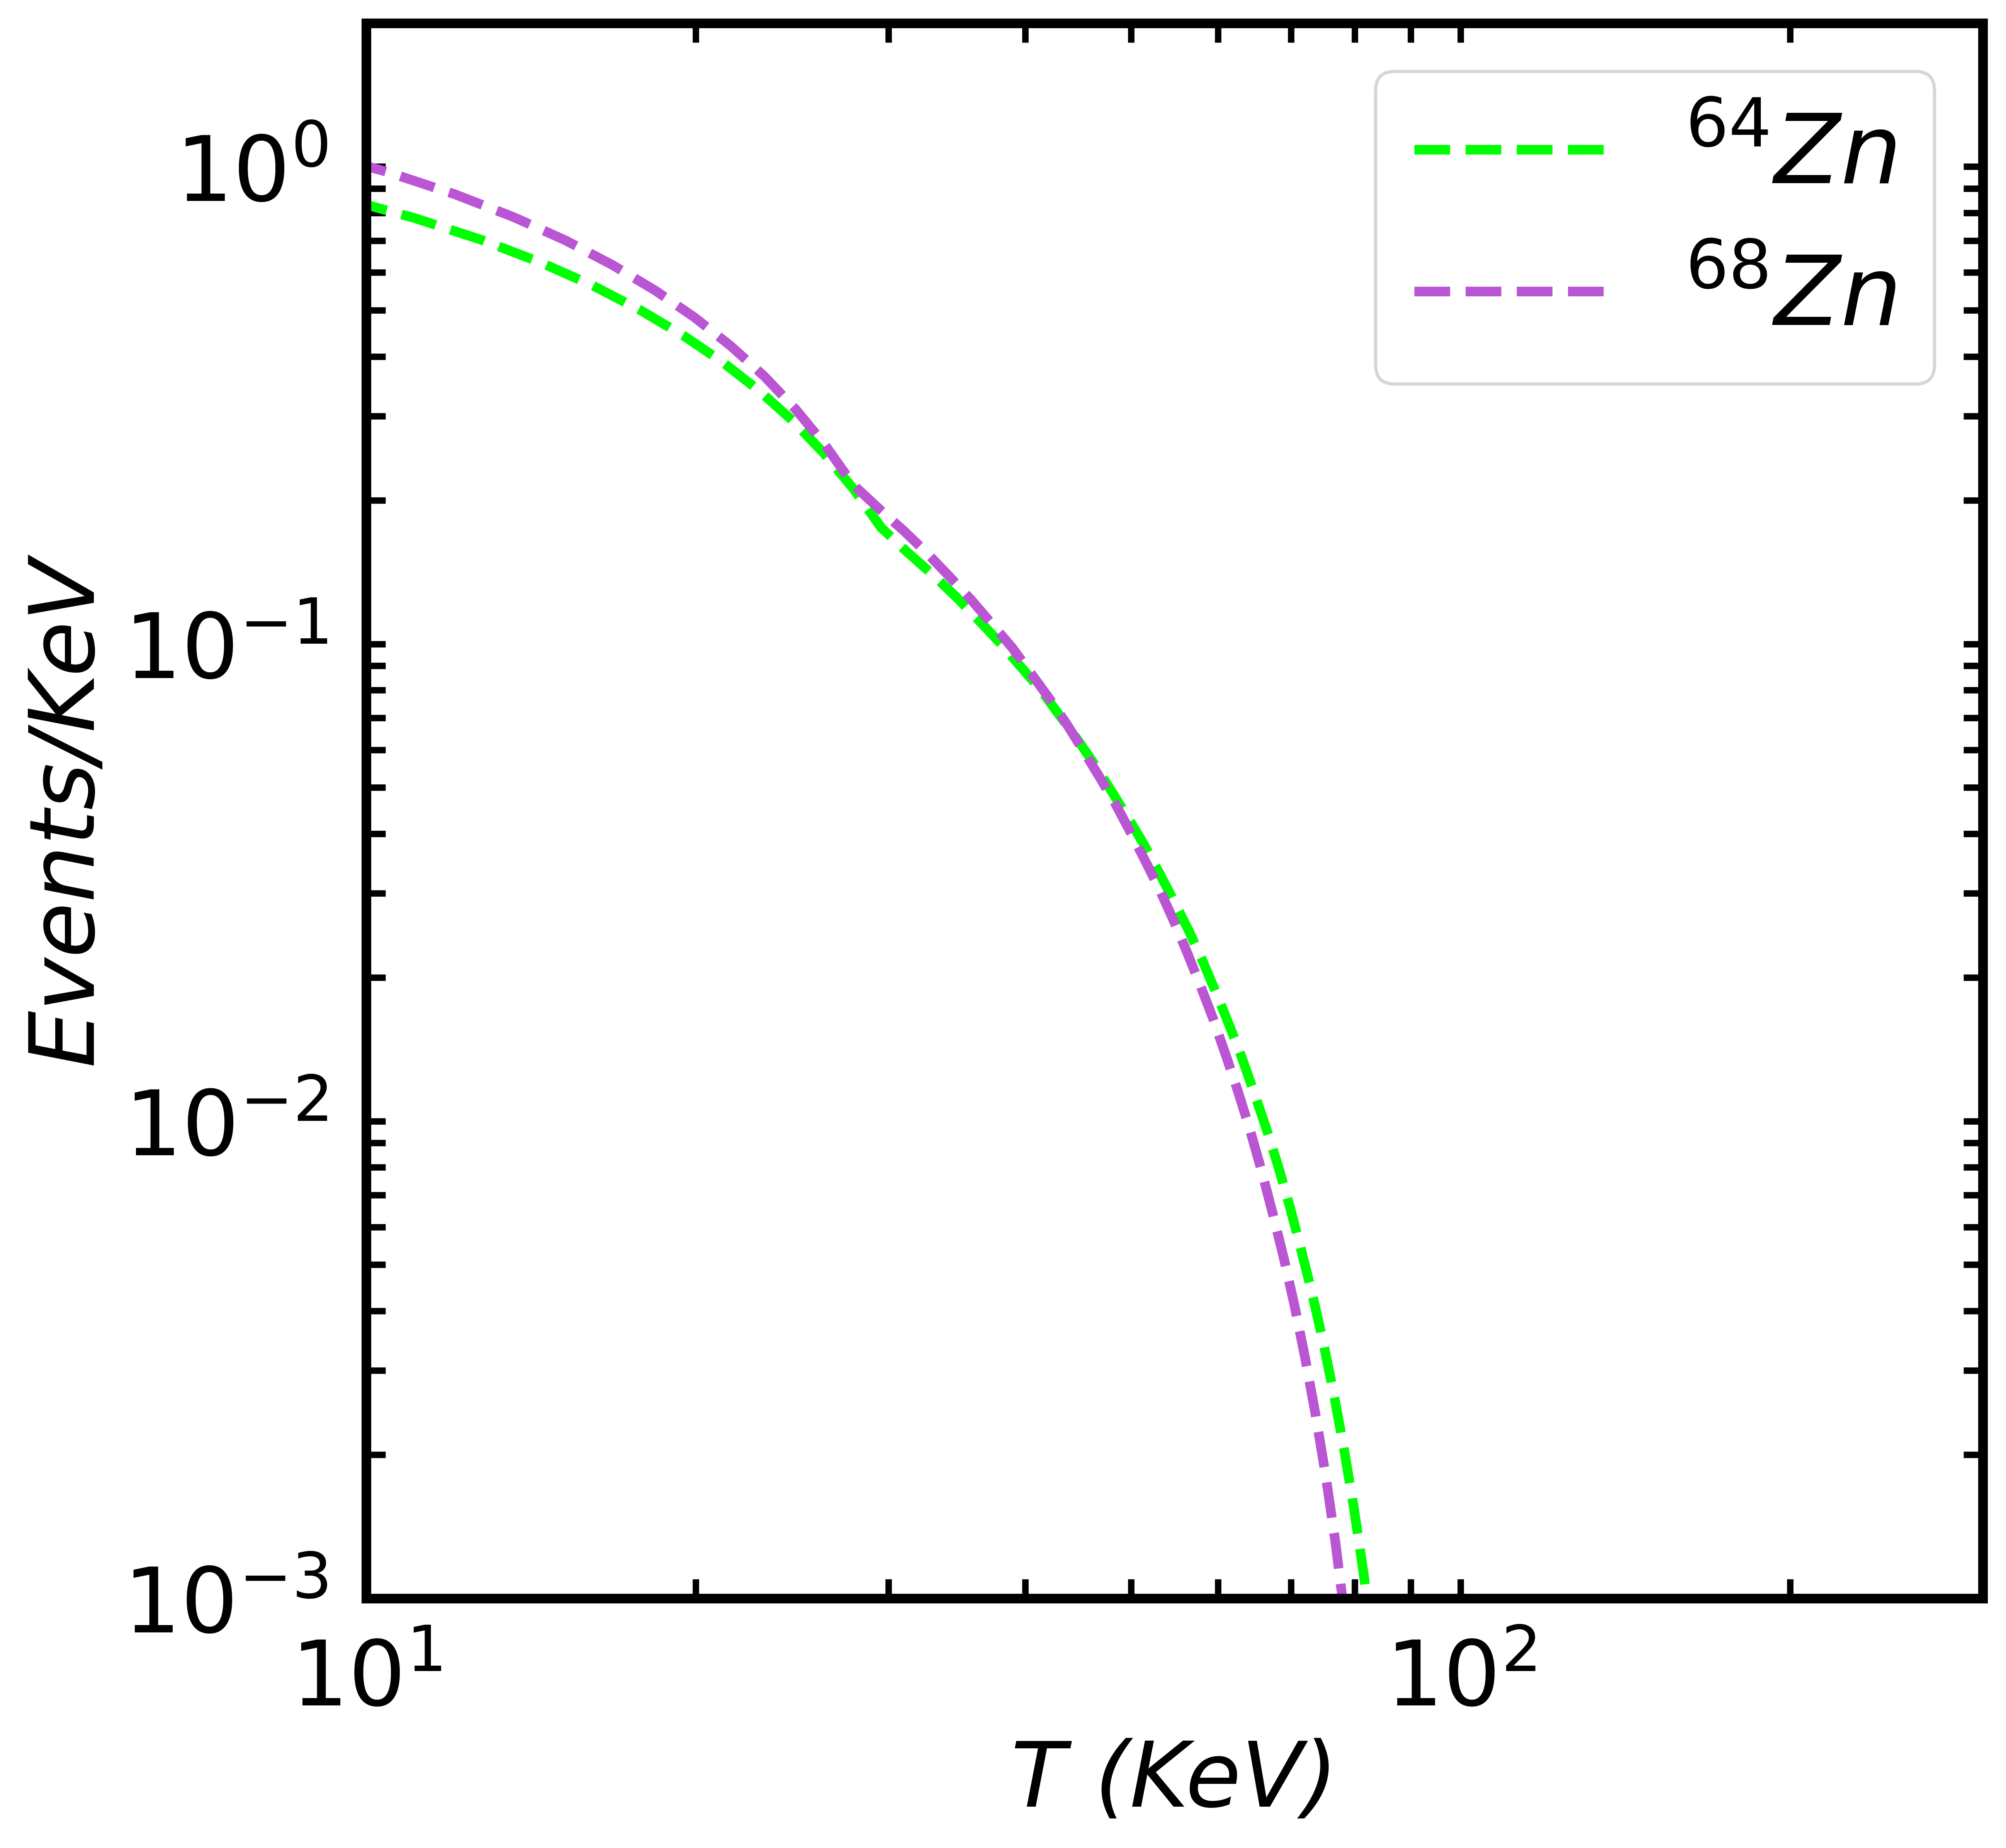
\includegraphics[scale=0.356]{figures/ZnRates.png}}\hspace{0em}%
     \subfigure{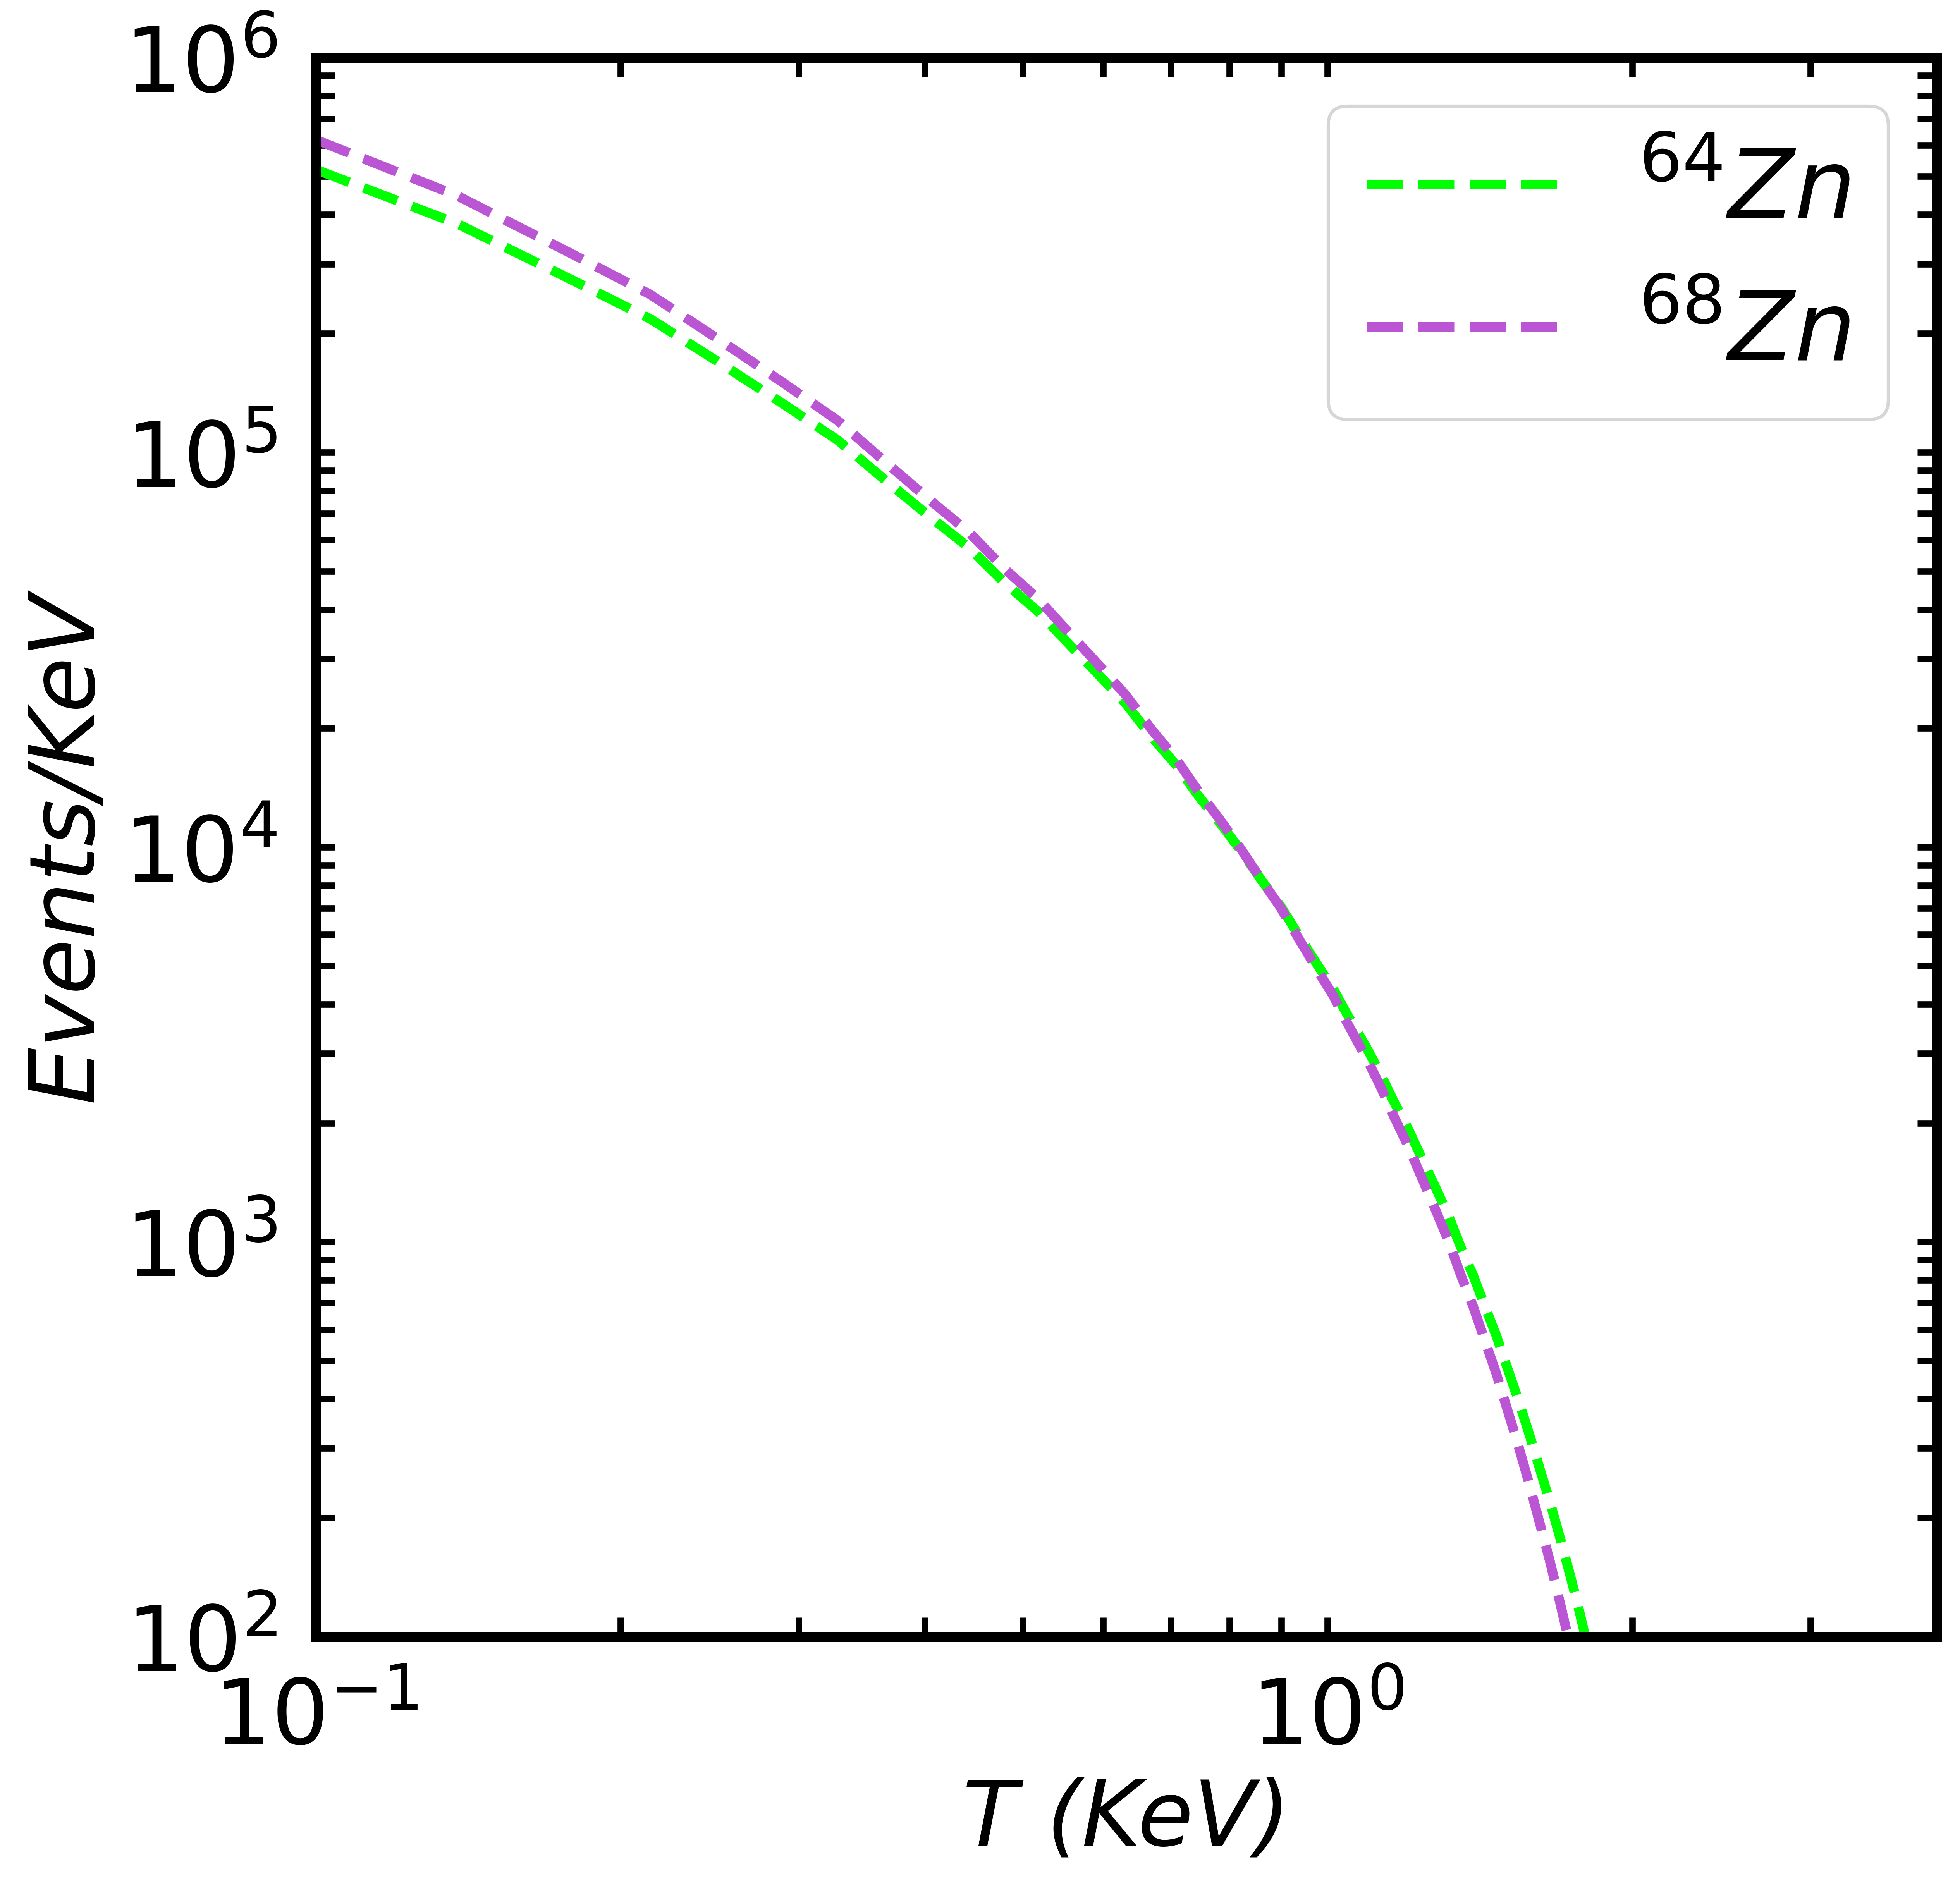
\includegraphics[scale=0.356]{figures/ReactorZn.png}}\par \vspace{0em}%
     \subfigure{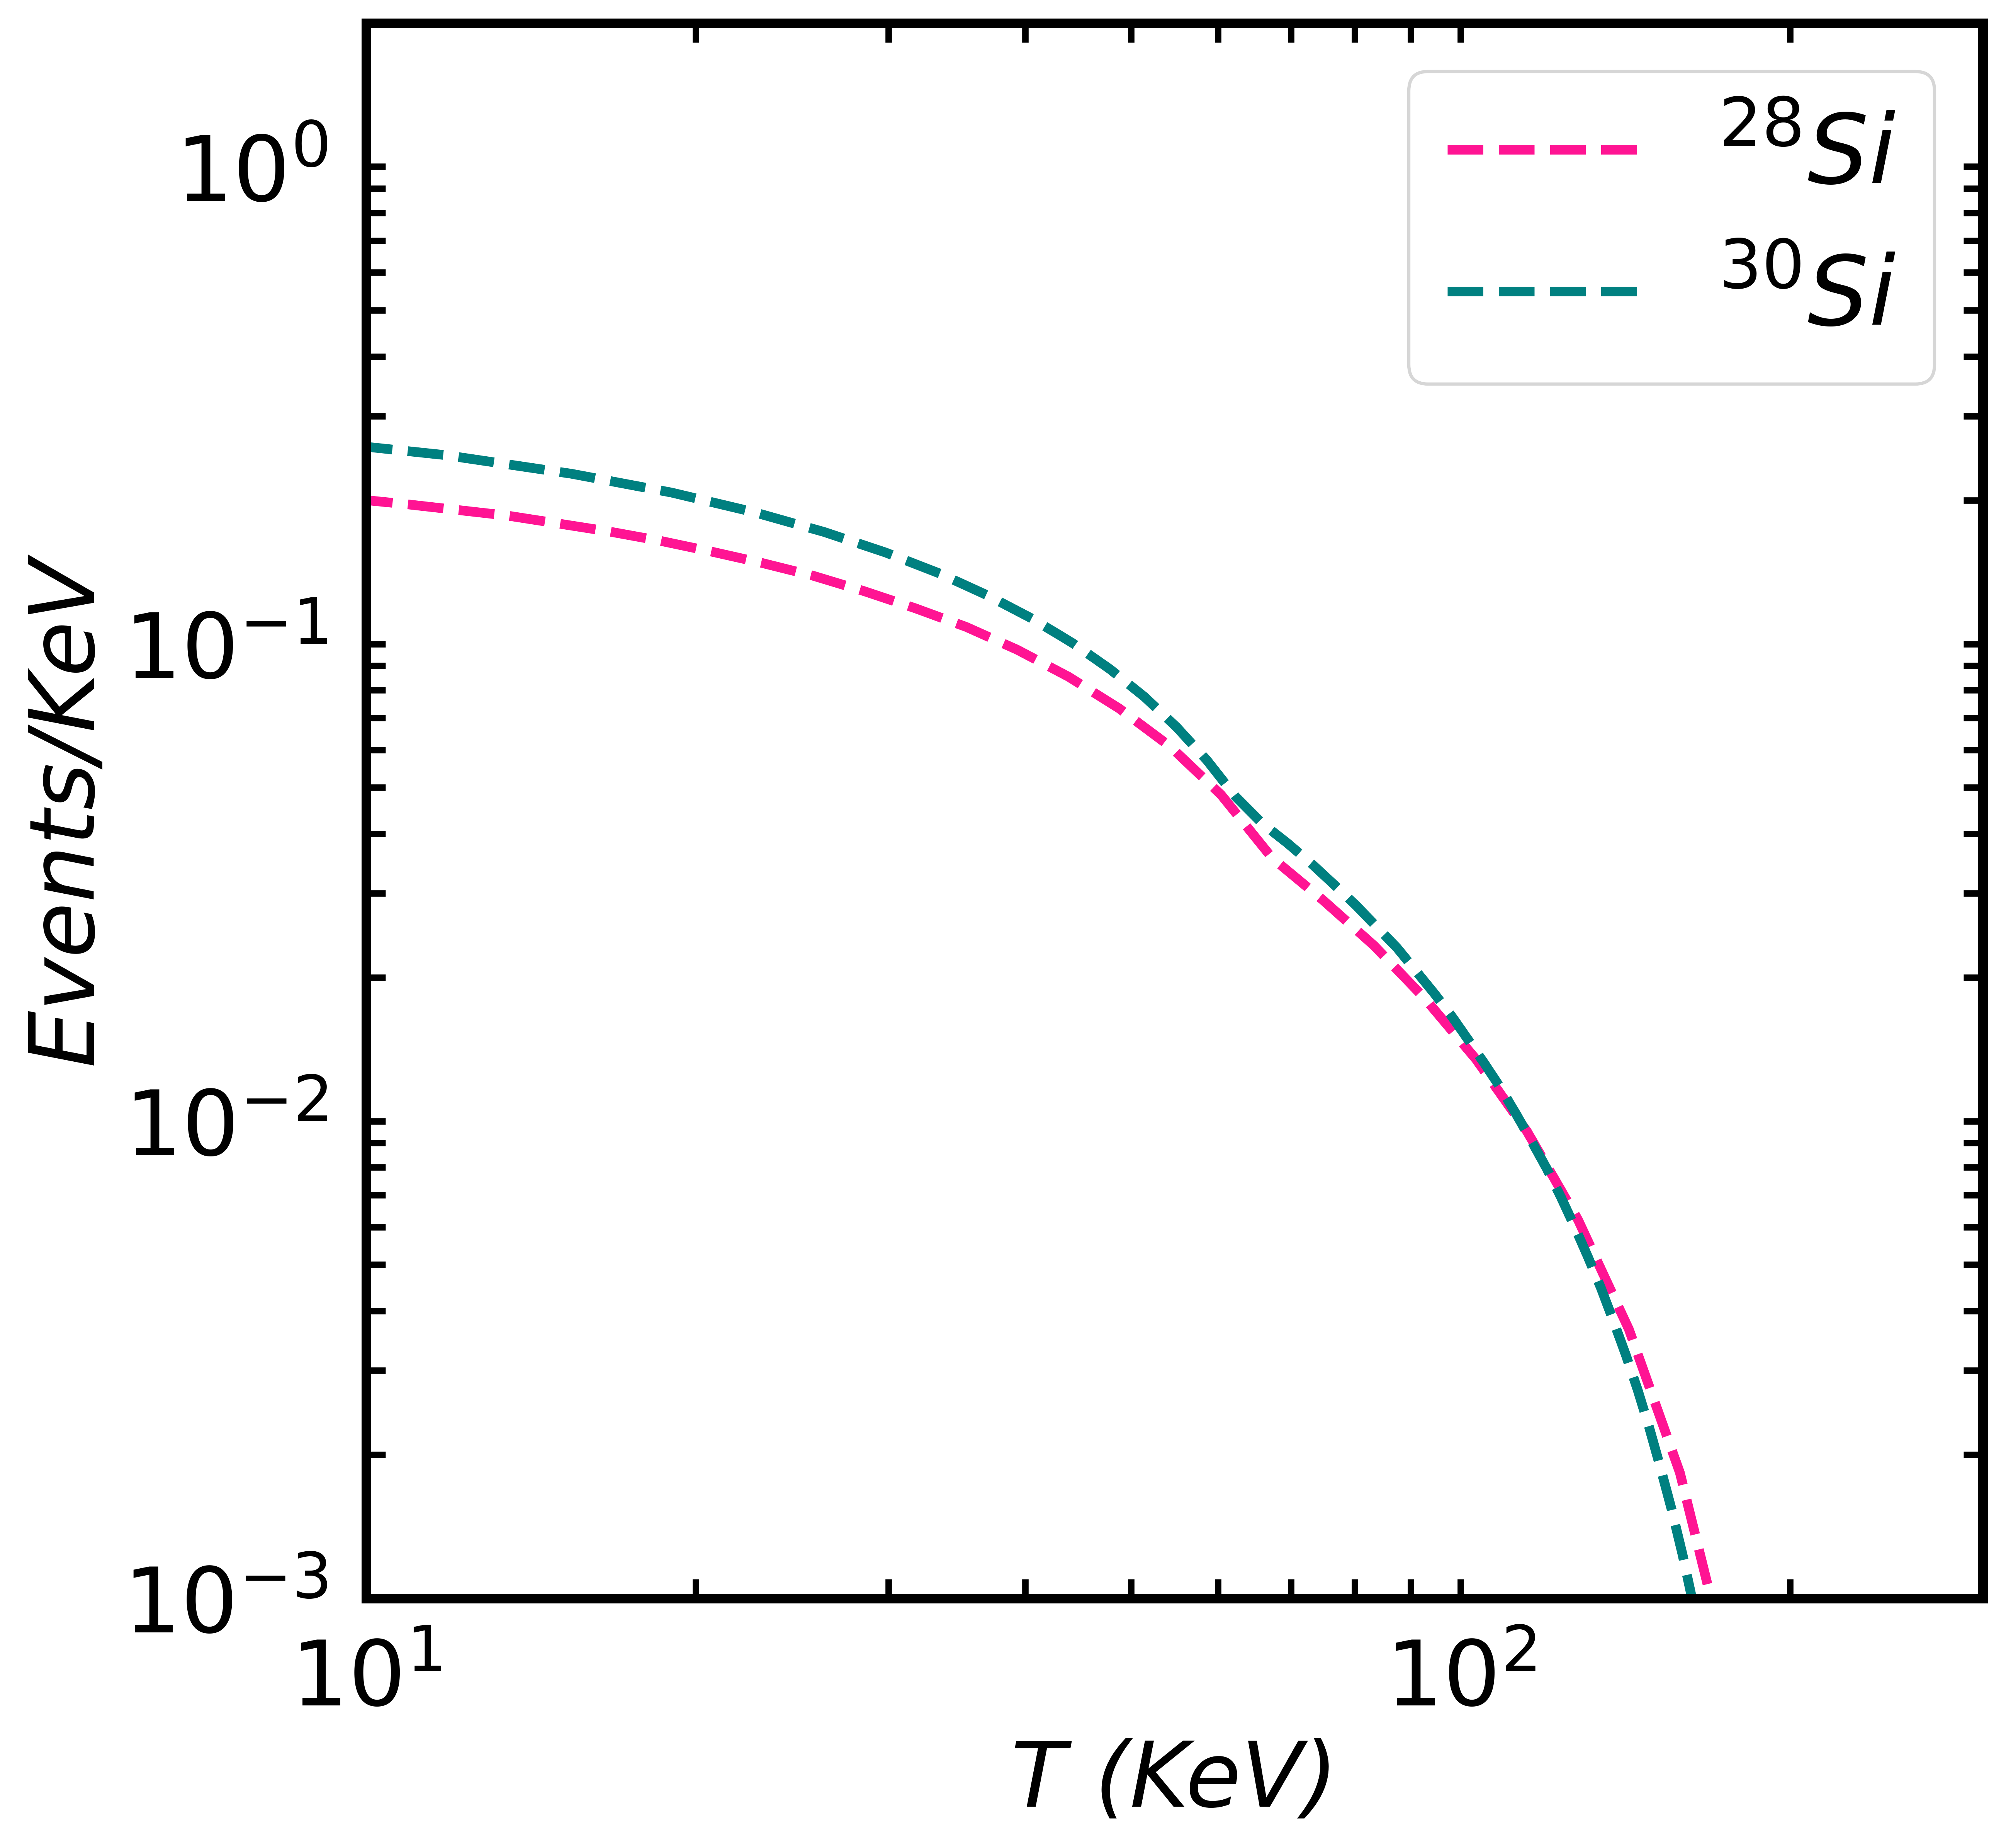
\includegraphics[scale=0.356]{figures/RatesSi.png}}\hspace{0em}%
     \subfigure{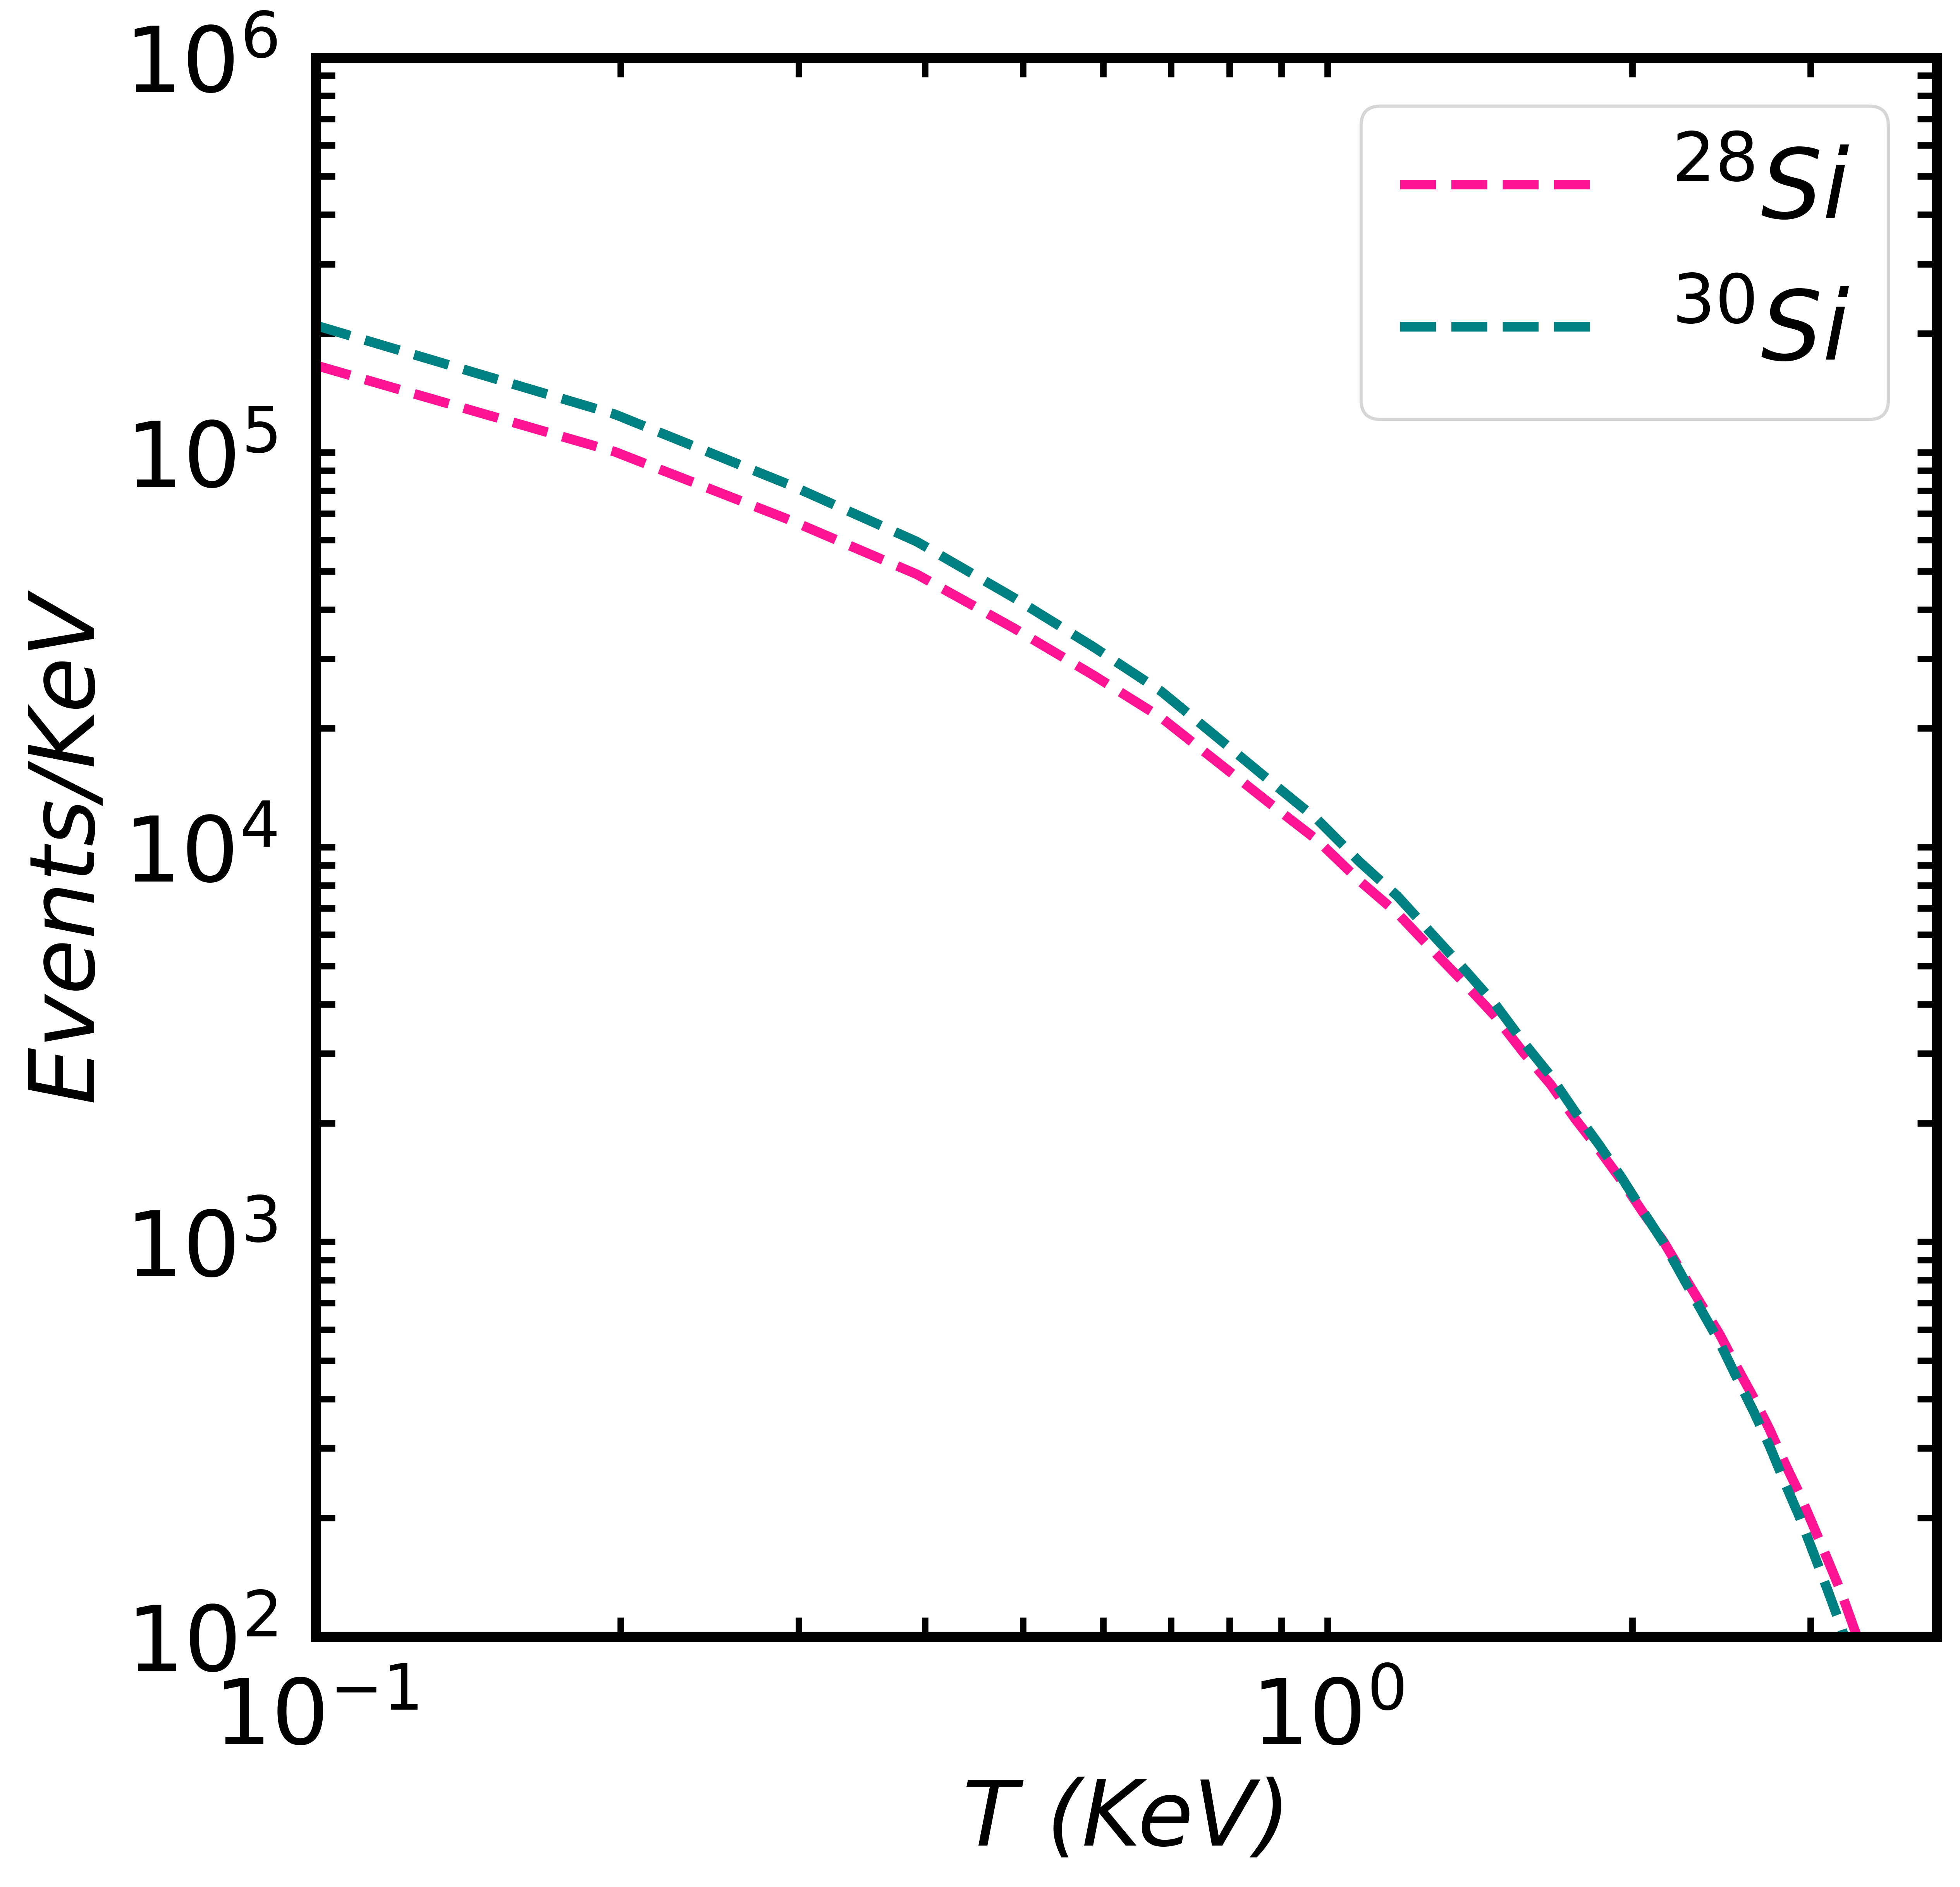
\includegraphics[scale=0.356]{figures/ReactorSi.png}}
     \caption{Differential event rate in terms of the nuclear recoil. The top panel refers to Zn isotopes, and the lower panel refers to Si isotopes. The detectors are exposed to $\pi$-DAR neutrino source in the left panels and to the antineutrino flux from the reactor in the right panels.}
     \label{fig8}
\end{figure}


As mentioned, the cross-section of Coherent Elastic Neutrino-Nucleus Scattering (CEvNS) exhibits a distinct relationship with the quadratic number of neutrons in the target material. Consequently, an isotope with a higher neutron number is anticipated to yield more events than one with fewer neutrons. However, it is essential to note that this expectation holds only when considering the entire spectrum of kinetic recoil energy. Unfortunately, this analysis poses challenges for current detectors due to variations in their thresholds and efficiencies, making it difficult to accurately capture the entire energy range.

In Figure \ref{fig8}, the differential event rate can be observed, comparing different detectors of Si and Zn exposed to $\pi$-DAR source (left panel) and reactor flux (right panel). In both scenarios, a specific point exists towards the end of the energy spectrum where the differential rates of different isotopes intersect. This outcome is anticipated because heavier nuclei have a lower limit on the kinetic energy they can reach. As a result, there are specific regions of recoil energy where, despite the dependence on $N^2$, a target with fewer neutrons would observe more events.

\section{Testing the $N^2$ dependence}
The total number of events calculated in the last chapter can be used to make a $\chi^2$ test by minimizing the function
\begin{equation}
    \chi^2=\sum_{ij}\left(\mathcal{N}_i^{theo}-\mathcal{N}_i^{exp}\right)\left[\sigma_{ij}^2\right]^{-1}\left(\mathcal{N}_j^{theo}-\mathcal{N}_j^{exp}\right),
    \label{Chi}
\end{equation}
where $\sigma_{ij}^2$ is the covariant matrix and the indices $i$ and $j$ run over the number of detectors. In our case, we have two detectors for each material, so the covariance matrix is a 2$\times$2 matrix with nonzero elements outside the diagonal due to the correlation between the detectors.

\begin{equation}
    \sigma^2=\begin{pmatrix}
              \sigma_l^{{stat}^2}+\sigma_l^{A^2}+\sigma_l^{B^2} & \sigma_l^{stat}\sigma_m^{stat}+\sigma_l^A\sigma_m^A+\sigma_l^B\sigma_m^B\\
              \sigma_l^{stat}\sigma_m^{stat}+\sigma_l^A\sigma_m^A+\sigma_l^B\sigma_m^B & \sigma_m^{{stat}^2}+\sigma_m^{A^2}+\sigma_m^{B^2}
              \end{pmatrix}.
\end{equation}
\\
Let A and B represent the primary sources of errors within the experiment: Quenching factors (A) and form factors (B), with $\sigma^A$ and $\sigma^B$ their corresponding uncertainties. And $\sigma^{stat}$  represents the statistical error of the detectors.

$\mathcal{N}^{exp}$  is the ``experimental" number of events, which is calculated as presented in the previous chapter by the following double integration

\begin{equation}
    \mathcal{N}=N_D\int_T A(T) dT \int_{E_{\nu,min}}^{E_{\nu,max}} \frac{dN_\nu}{dE} \frac{d\sigma}{dT} dE,
\label{N}
\end{equation}

with $N_D=t_{run}N_{targ}$, the effective number of target nuclei within the detector during the running time of the experiment,  A(T) an acceptance function, and we simplify the situation by setting it equal to one in the most basic scenario.

Table \ref{events} presents the results obtained for the total expected number of events for the Zn and Si detectors exposed to a $\pi$-DAR source for both a 1-year and a 5-year experiment duration. These values will be used as the $\mathcal{N}^{exp}$ in each case.
\\
\begin{table}[h]
\centering

 
\begin{tabular}{ p{3cm}p{3cm}p{3cm}  }
\toprule
    & 1 year & 5 years                               \\ \midrule
$^{64}Zn$ & 17.2384      & 86.1922                                              \\
$^{68}Zn$ & 20.1694      &  100.847   \\
           &              \\
$^{28}Si$ & 7.53392      &    37.6696                              \\
$^{30}Si$ & 9.21781     & 46.0891                                     \\ \bottomrule
\end{tabular}
 \caption{number of events for the detectors exposed to a $\pi$-DAR source}
\label{events}
\end{table}


In order to test the dependence on $N^2$, we first expand the quadratic term in the cross-section of CEvNS. Then, we proceed by substituting the number of neutrons (N) with a variable factor N'. This will measure the deviation of an experimental measurement from the expected quadratic dependence. 
By substituting this expanded cross-section into equation (\ref{N}), organizing and separating terms, we can express the prediction of the number of events $\left(\mathcal{N}^{theo}\right)$  as follows:

\begin{equation}
\begin{split}
\mathcal{N}^{theo}
&=\phantom{-}Z^2g_p^{V^2}N_D\frac{G_f^2 M}{2\pi}\int_{T}A(T)dT\int_{E_{\nu,min}}^{E_{\nu,max}} \frac{dN_\nu}{dE} \left[2-\frac{MT}{E_\nu^2}\right]F_z^2(q^2) dE \\
&\quad\smash[b]+2N'\left(Zg_p^Vg_n^VN_D\frac{G_F^2 M}{2\pi}\int_T A(T) dT \int_{E_{\nu,min}}^{E_{\nu,max}} \frac{dN_\nu}{dE} \left[2-\frac{MT}{E_\nu^2}\right] F_z(q^2)F_N(q^2) dE\right) \\
&\quad\smash[b]+N'^2\left(g_n^{V^2}N_D\frac{G_F^2 M}{2\pi}\int_{T}A(T)dT\int_{E_{\nu,min}}^{E_{\nu,max}}\frac{dN_\nu}{dE} \left[2-\frac{MT}{E_\nu^2}\right] F_N^2(q^2) dE\right),
\end{split}
\end{equation}

with this information, we can now use equation (\ref{Chi}) to test the sensitivity of these detectors to the quadratic dependence of the number of neutrons. This sensitivity analysis helps us assess the capability of the detectors to accurately measure and distinguish the quadratic dependence of the number of neutrons in Coherent Elastic Neutrino-Nucleus Scattering experiments.
\begin{figure}[h!]
\centering
\subfigure[\emph{1 year of run time}]{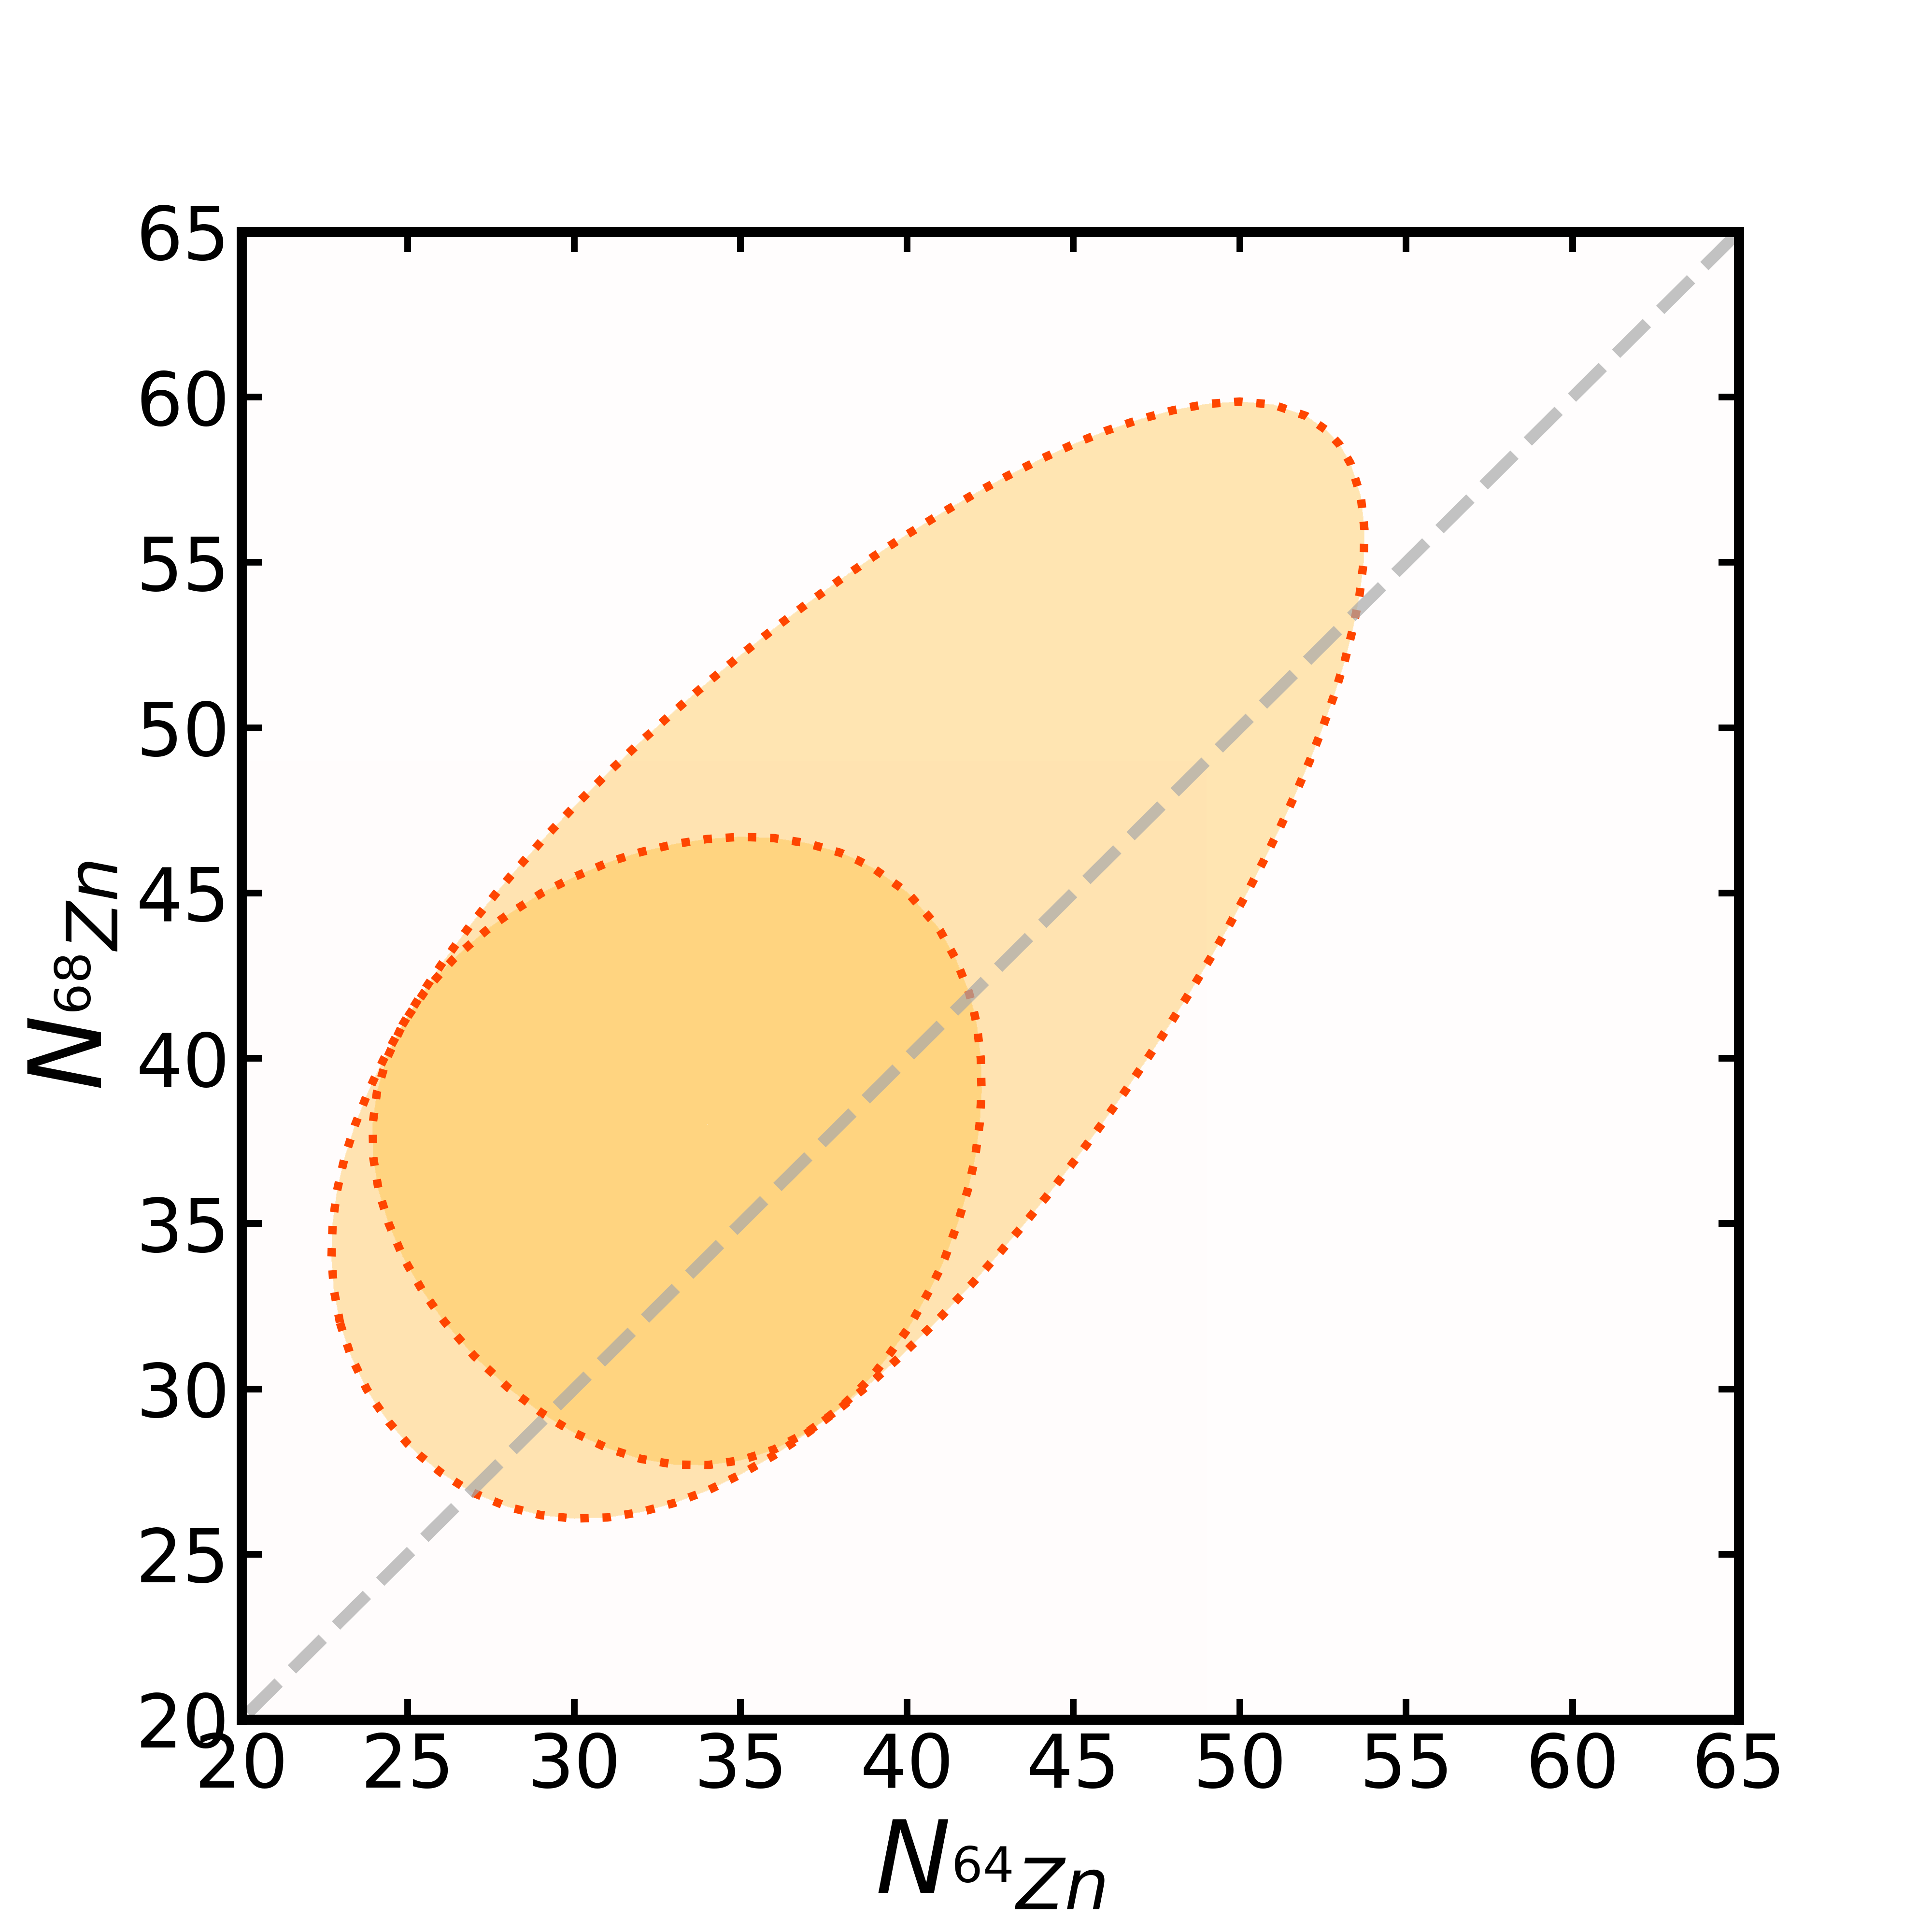
\includegraphics[scale=0.35]{figures/Zn1Año.png}}\hspace{-1em}%
\subfigure[\emph{5 years of run time}]{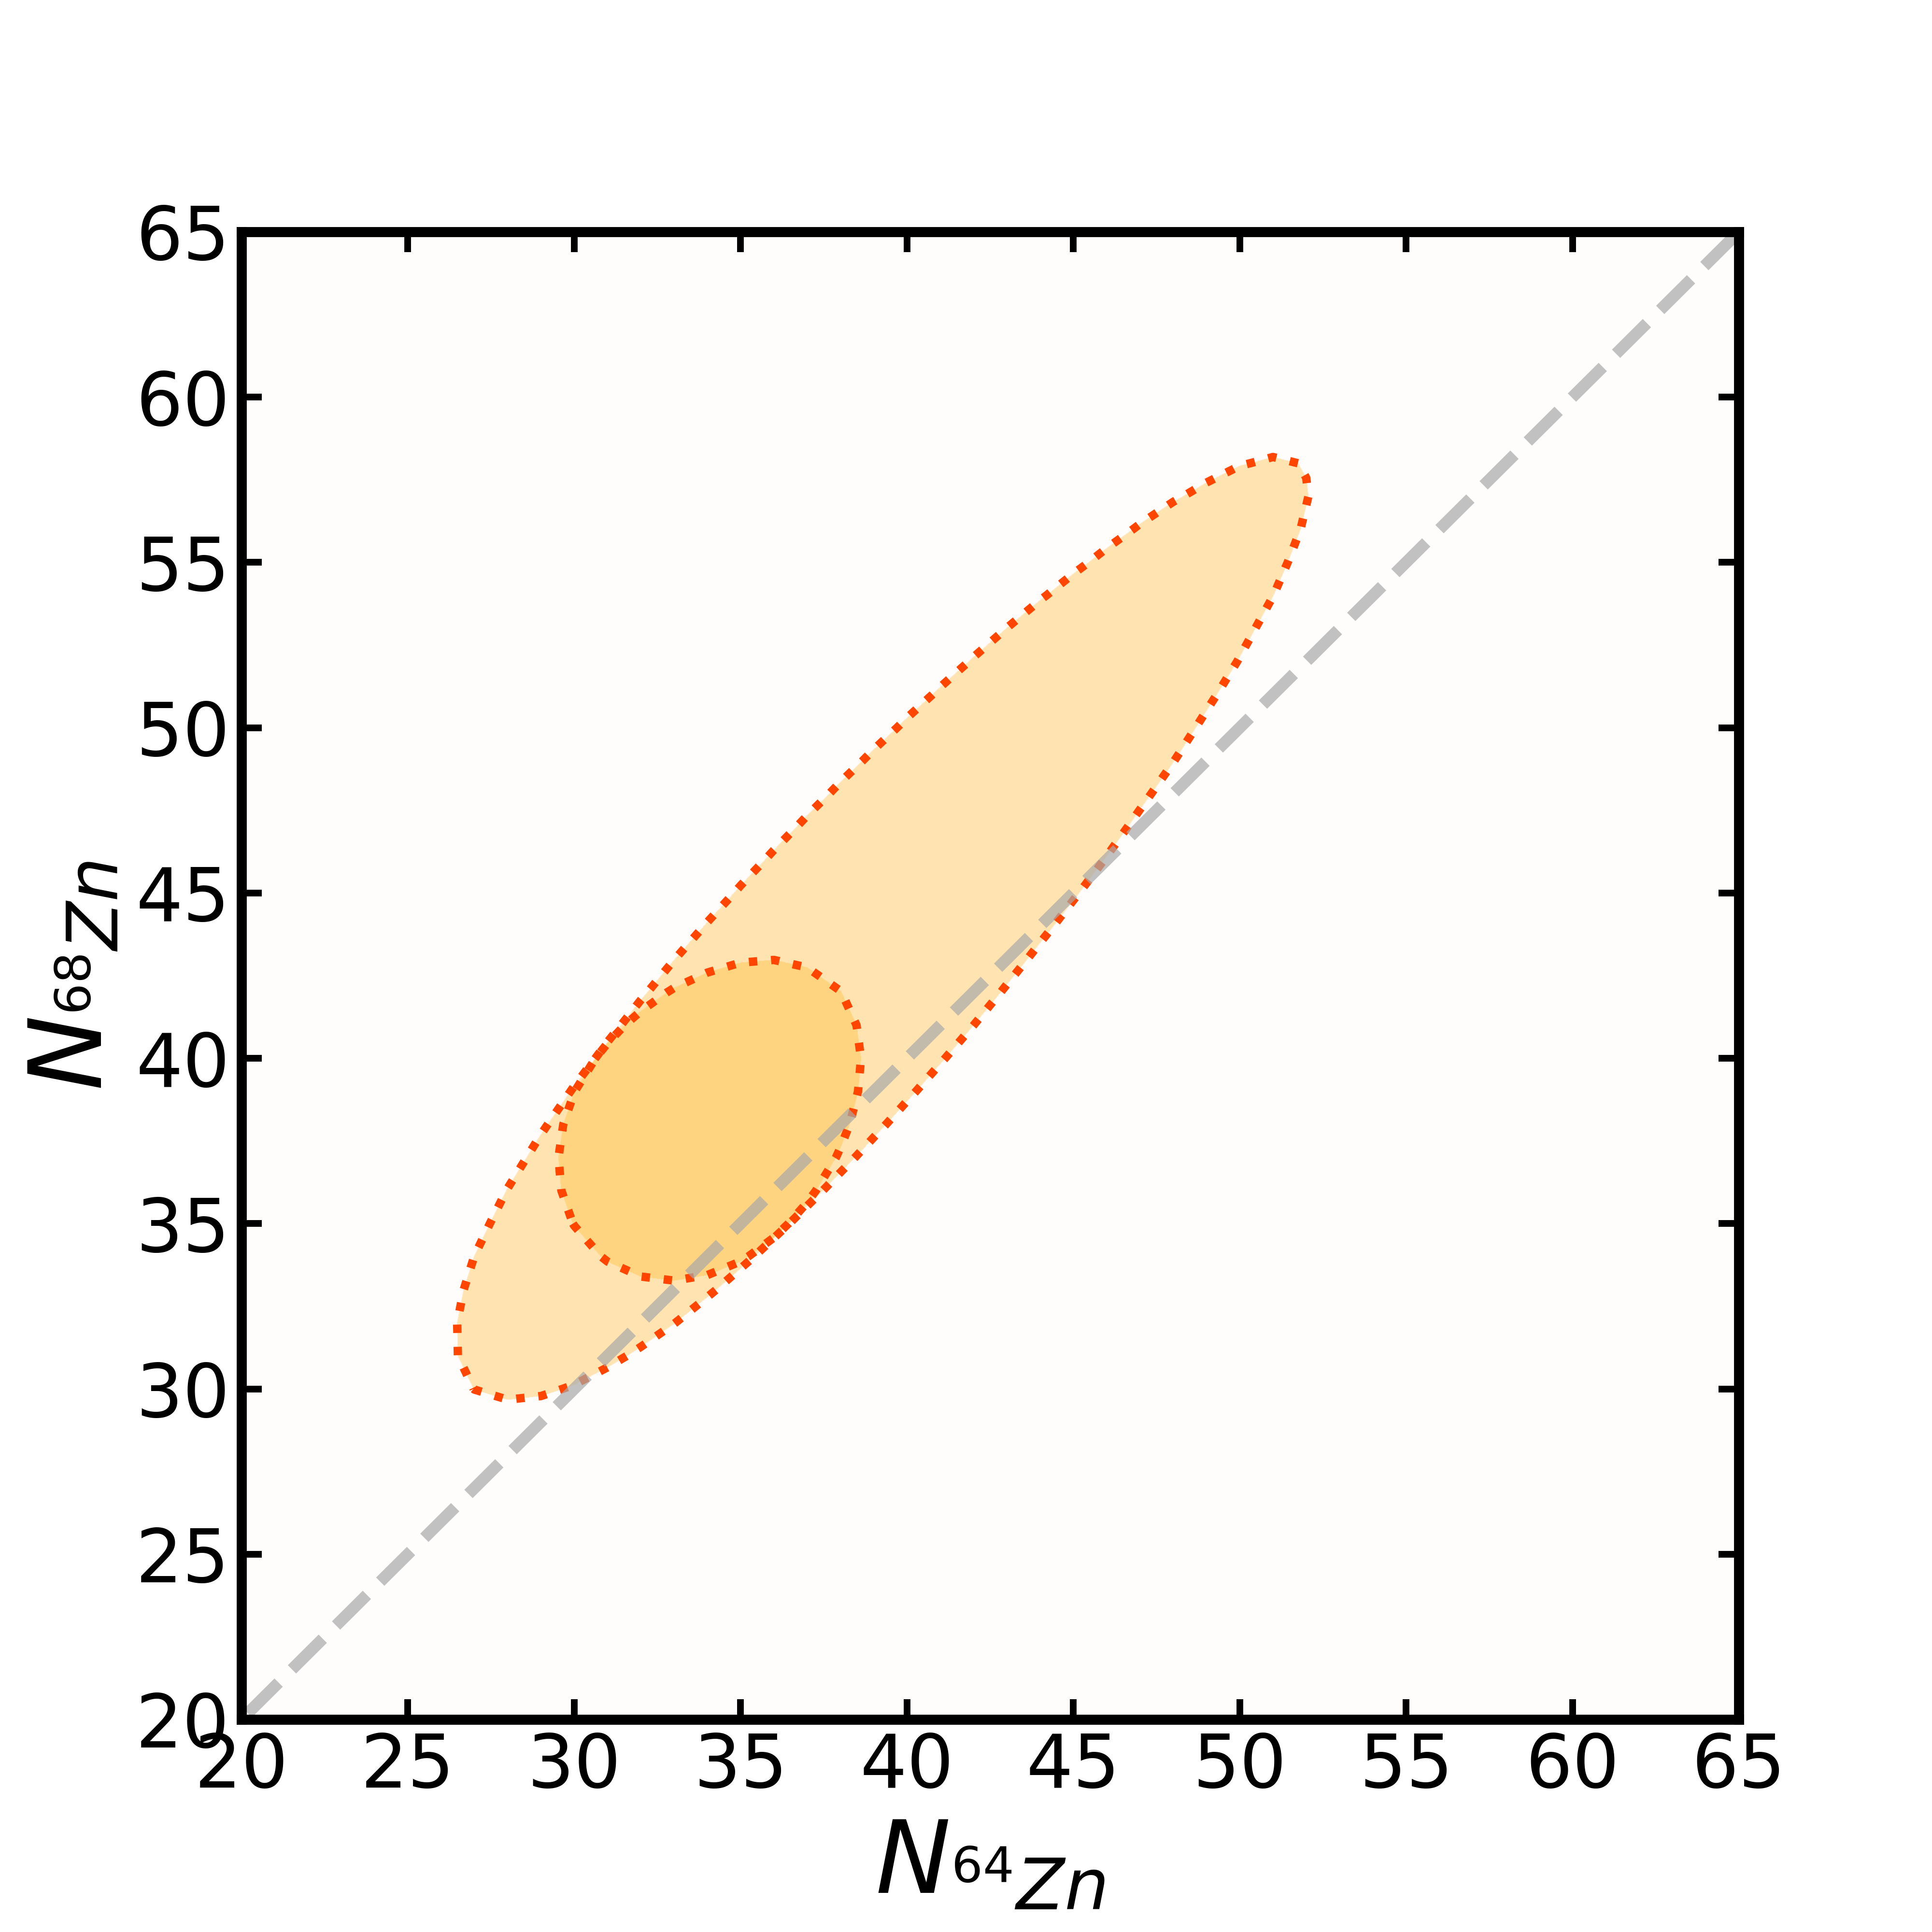
\includegraphics[scale=0.35]{figures/Zn5Año.png}}
     \caption{Expected allowed values of the N' factor at a 90$\%$ confidence level for Zn isotopes detector exposed to $\pi$-DAR neutrino beam at different experiment run times. Light regions refer to the case of $\sigma_A = 25\%$ and $\sigma_B=10\%$ while dark regions refer to the case of $\sigma_A=\sigma_B=5\%$.}
     \label{N2Zn}
\end{figure}

Using a flux from the SNS ($\pi$-DAR source), figure \ref{N2Zn} displays the expected allowed values that are compatible with an $N^2$ dependence for $^{68}Zn$ on the vertical axis and $^{64}Zn$ on the horizontal axis. Each detector had a mass of 1 kg, and two experiment run time cases were considered: 1 year and 5 years.
Similarly, the analysis was carried out for Silicon isotopes, presented in Figure \ref{N2Si}. $^{30}Si$ is represented on the vertical axis, while $^{28}Si$ is depicted on the horizontal axis.

It was considered a scenario where the contribution of the systematic uncertainty coming from the quenching factor and the form factor is $25\%$ and $10\%$, respectively, shown in the light area of the plots. The optimistic scenario where the contribution of these uncertainties is $5\%$ each is shown in the dark regions of the plots.

As depicted in the figures, the expected region forms an ellipse, indicating that the values of N' are restricted and exhibit a correlation with each other according to the $N^2$ rule.

\begin{figure}[h!]
\centering
\subfigure[\emph{1 year of run time}]{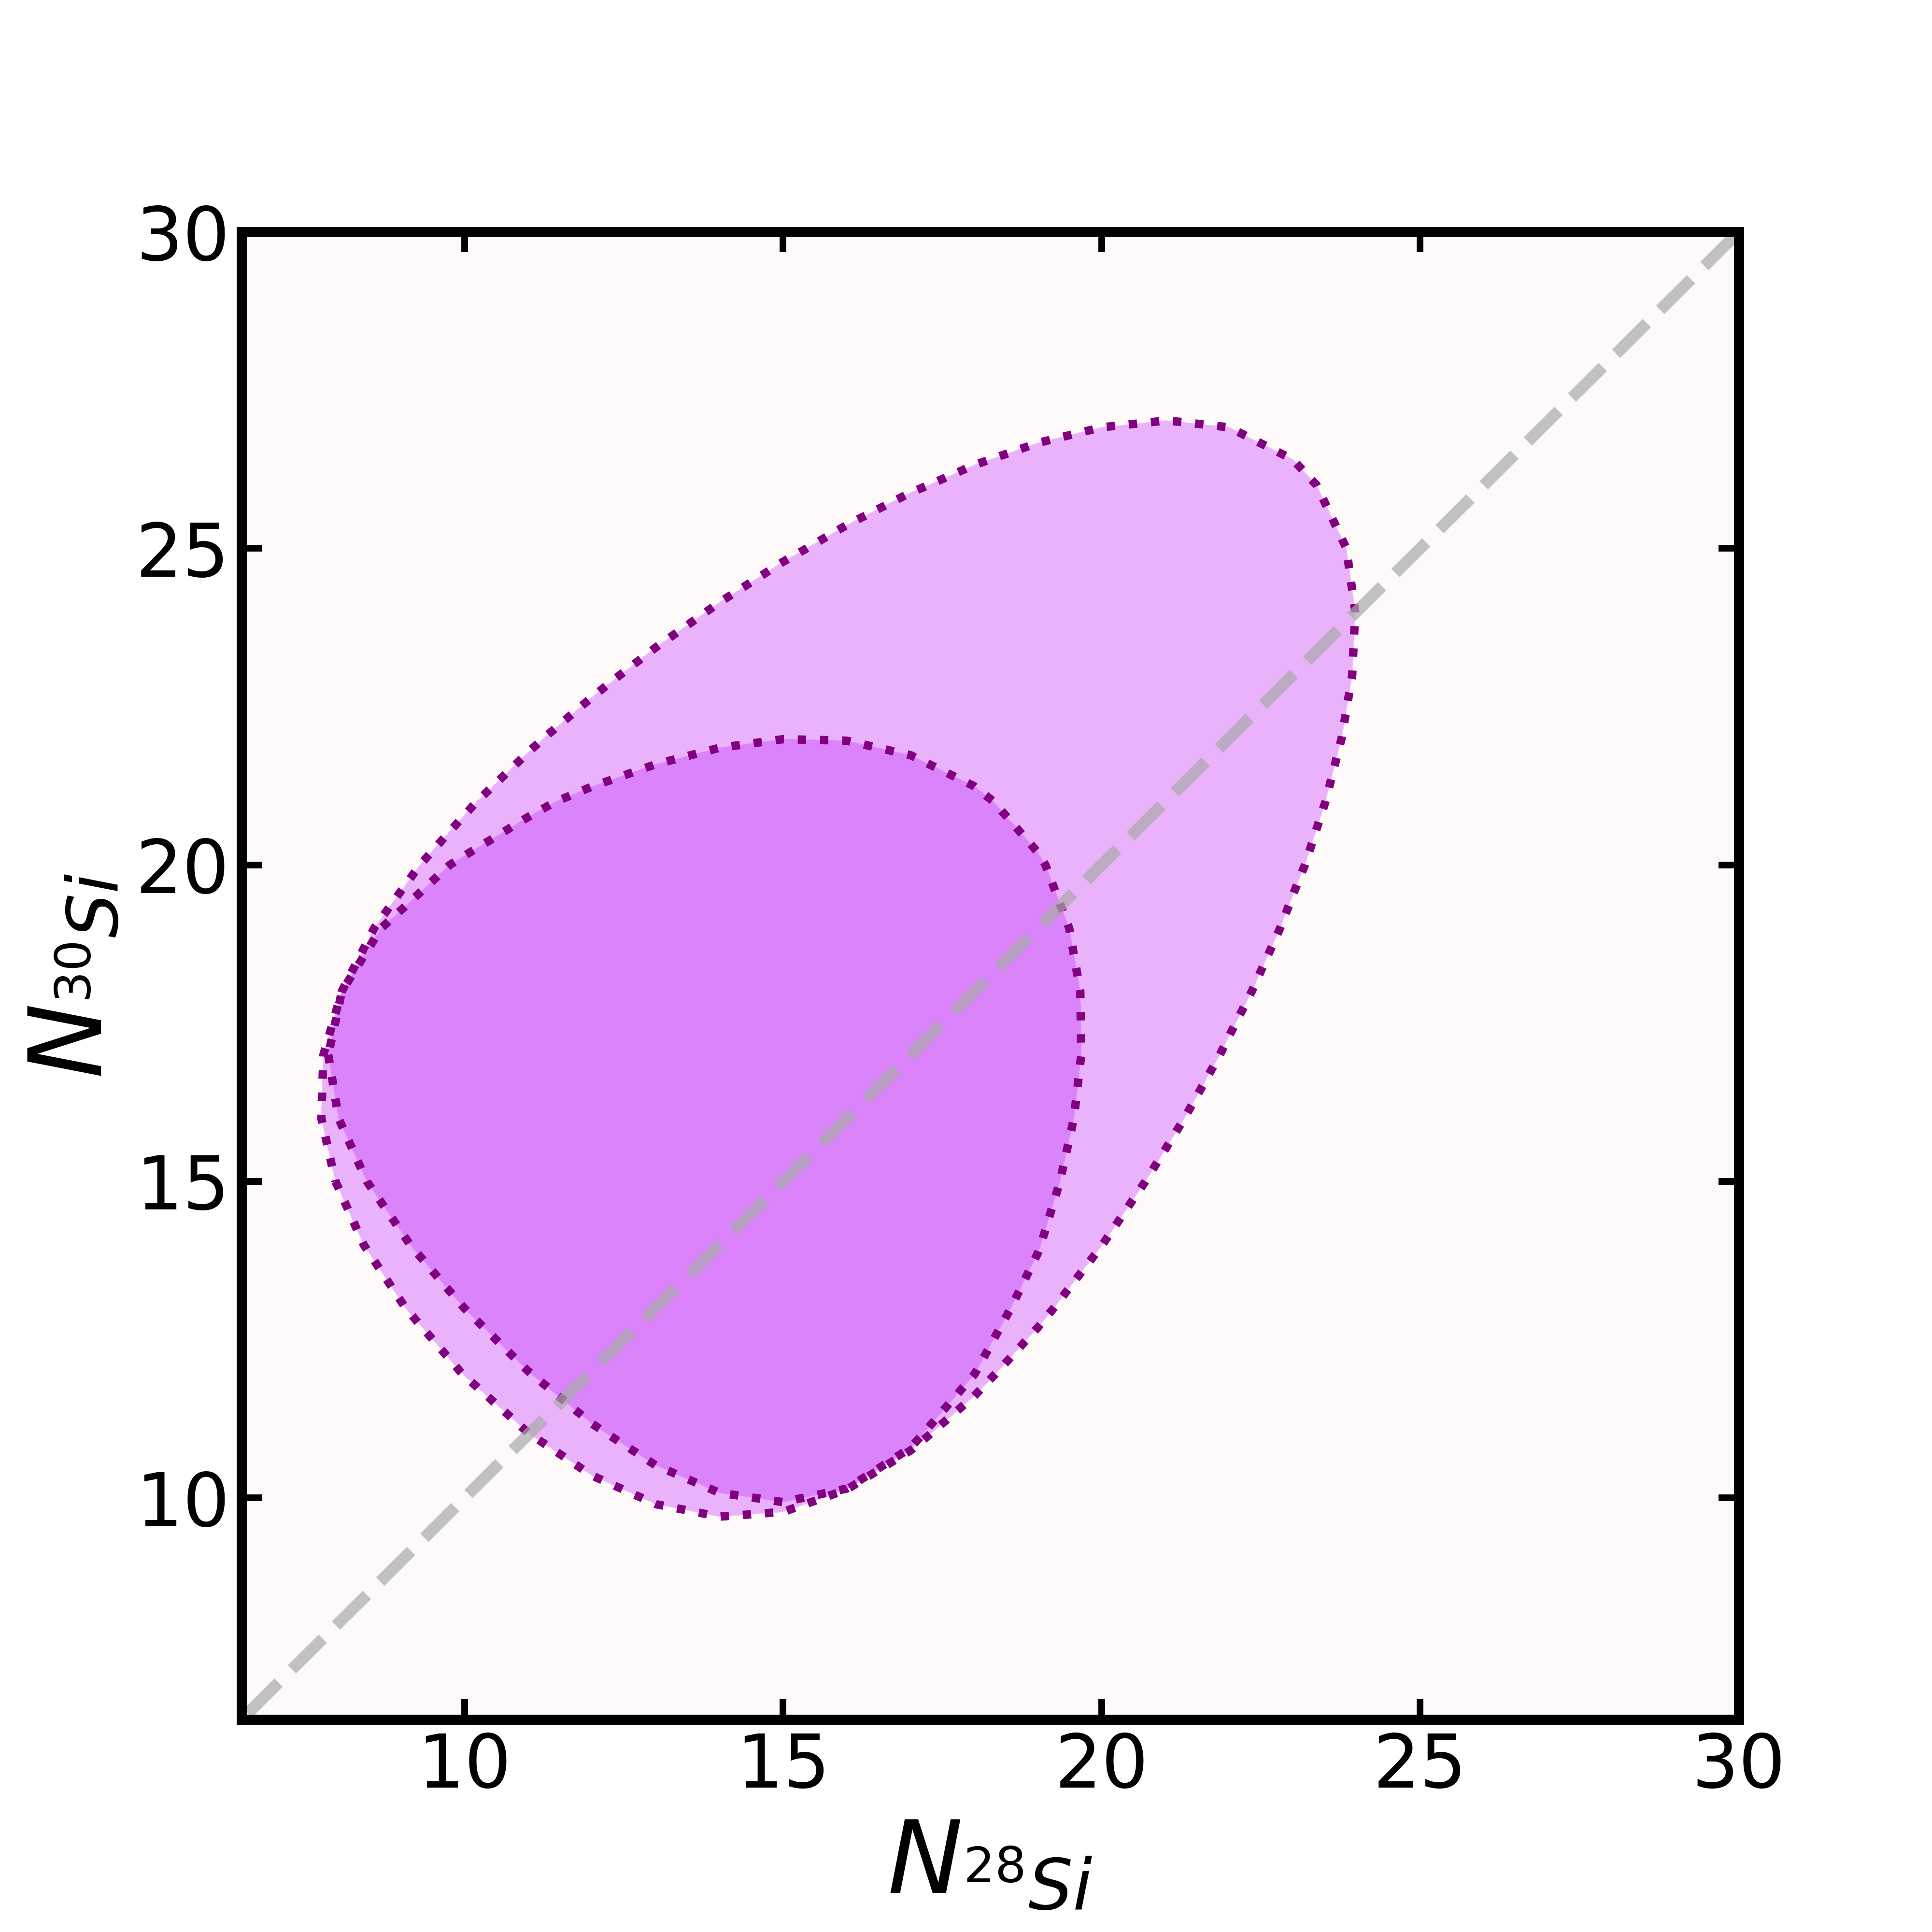
\includegraphics[scale=0.35]{figures/Si1Año.png}}\hspace{-1em}%
\subfigure[\emph{5 years of run time}]{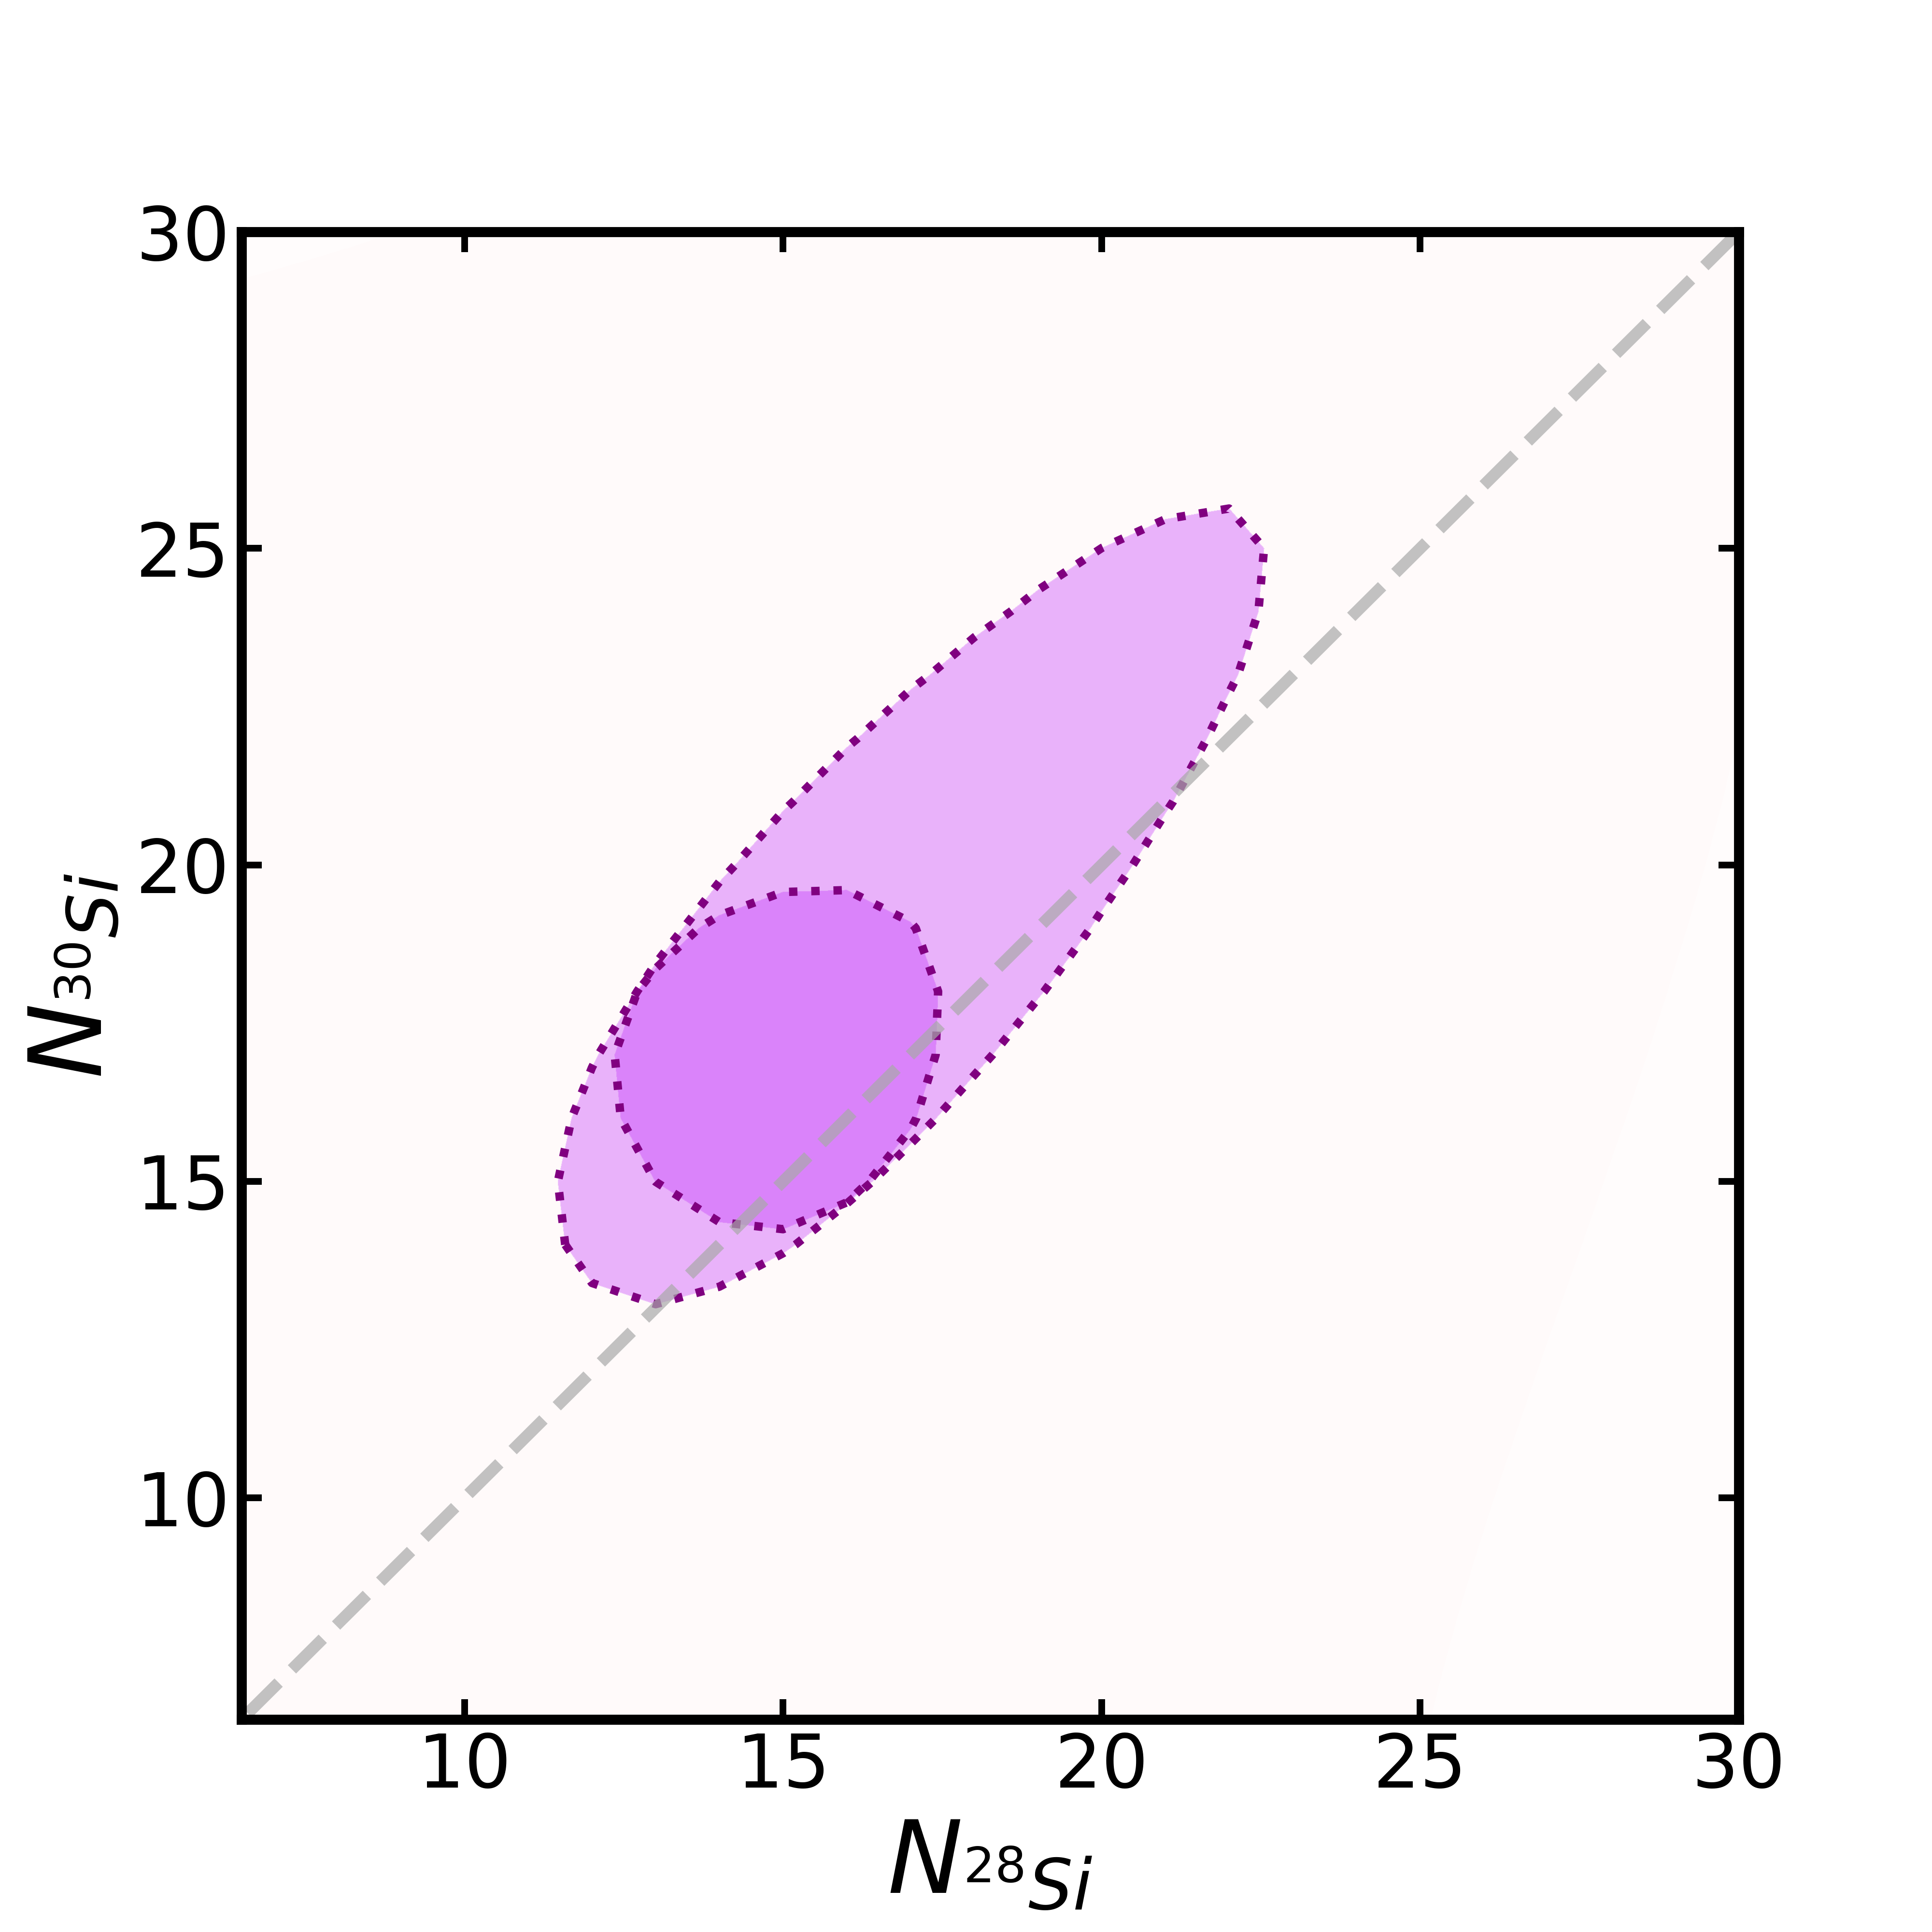
\includegraphics[scale=0.35]{figures/Si5Año.png}}
     \caption{Expected allowed values of the N' factor at a 90$\%$ confidence level for Si isotopes detector exposed to $\pi$-DAR neutrino beam at different experiment run times. Light regions refer to the case of $\sigma_A = 25\%$ and $\sigma_B=10\%$ while dark regions refer to the case of $\sigma_A=\sigma_B=5\%$.}
     \label{N2Si}
\end{figure}

We proceed to perform this analysis now using the reactor antineutrinos as a source. 
For the case of Zinc, we considered a range of recoil energies from 1 to 2 KeV. This is because, in the differential event plot (figure \ref{fig8}) corresponding to the reactor flux, we can observe that this region is above the intersection point. Figure \ref{ZnReactor} shows the expected allowed values corresponding to $^{68}Zn$ on the vertical axis and $^{64}Zn$  on the horizontal axis, both exposed to reactor flux.\\
We can also observe the case in which the detectors are uncorrelated, that is, if we consider detectors made of different materials with different systematic errors. Dashed lines in the figure illustrate this. Correlation allows for a more restricted region of expected permitted values.
\begin{figure}[h!]
    \centering
    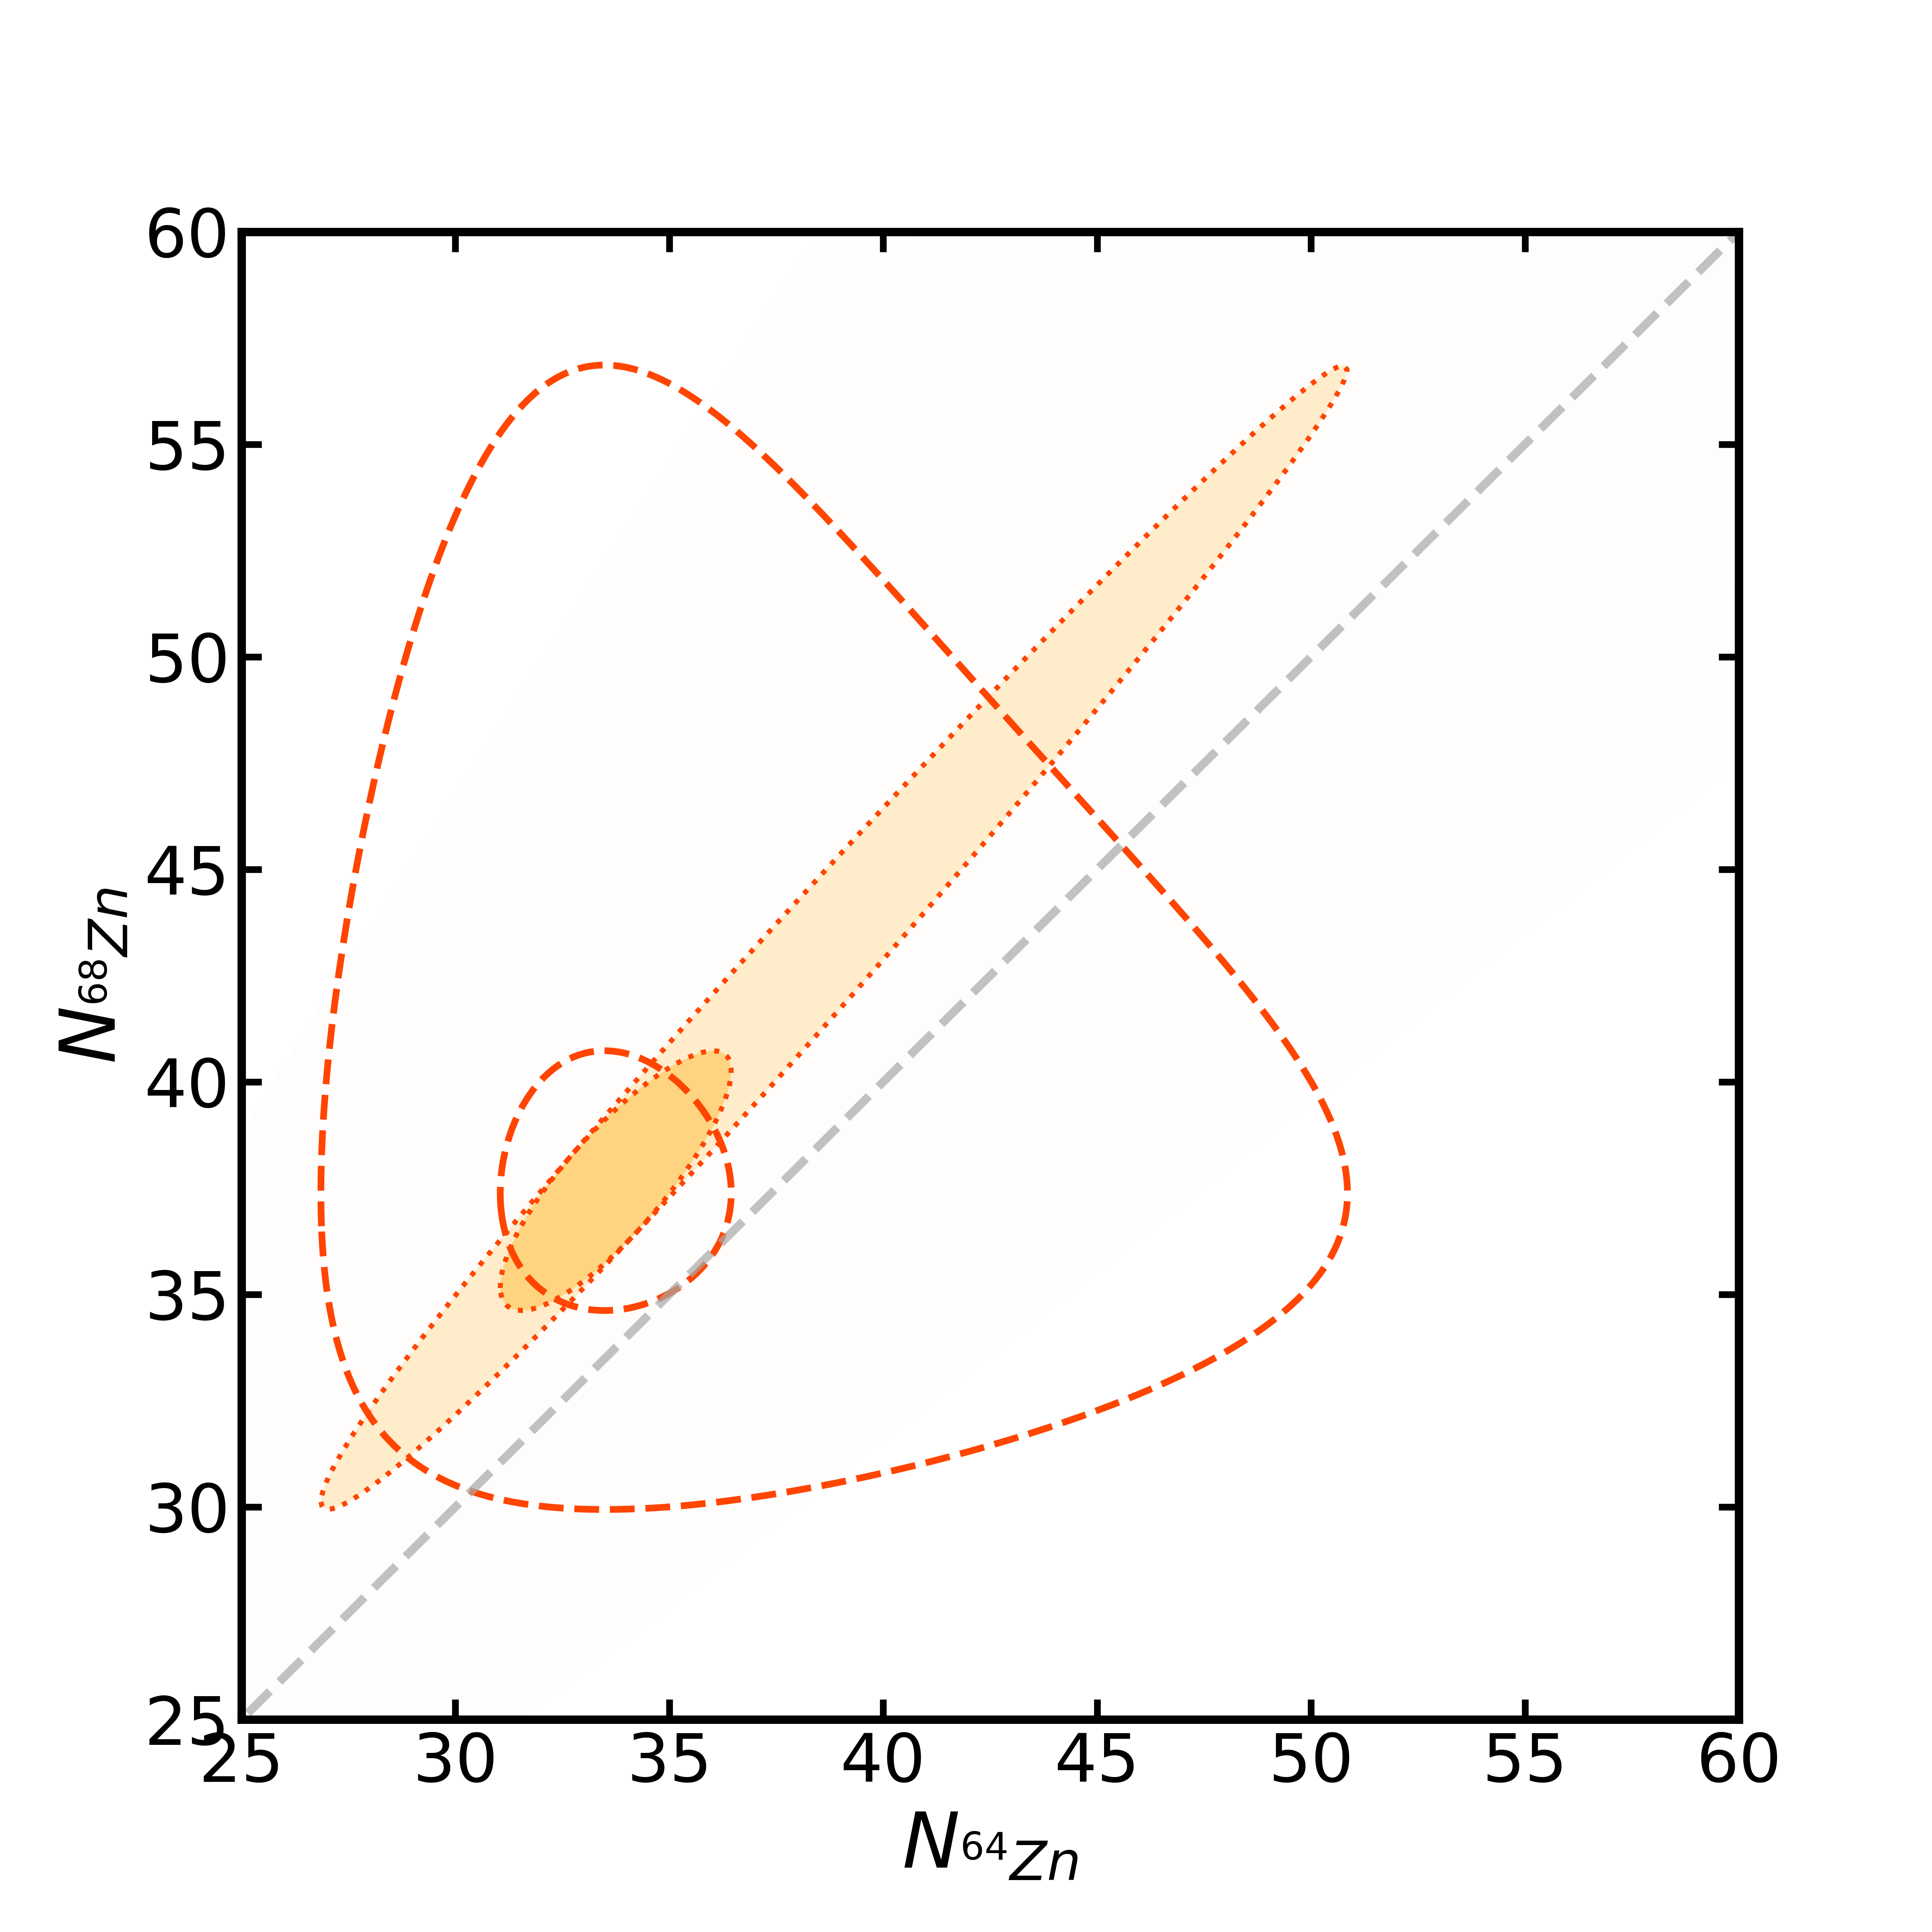
\includegraphics[scale=0.35]{figures/N2ZnNC.png}
\caption{Expected allowed values of the N' factor at a 90$\%$ confidence level for Zn isotopes detector exposed to reactor antineutrino flux with recoil energy from 1 - 2 KeV. Light regions refer to the case of $\sigma_A = 25\%$ and $\sigma_B=10\%$ while dark regions refer to the case of $\sigma_A=\sigma_B=5\%$. The uncorrelated case is also shown in dashed lines.}
    \label{ZnReactor}
\end{figure}
\\
In the case of Silicon, when observing the differential event rate corresponding to the reactor flux in figure \ref{fig8}, we notice that the intersection point is right in the recoil energy region between 1 - 2 KeV. For this reason, figure \ref{SiReactor} presents the expected allowed values for Si isotopes both in this range and in the 2 - 3 KeV range, which is above the intersection point. This allows for a better comparison with the case of Zinc.

In both cases, pi-DAR and reactor , it can be observed that the ellipse's width is dominated by statistical error. In the pi-DAR case, this is greater due to having a smaller number of events, while in the reactor case, a significant decrease in this error is evident. On the other hand, systematic errors determine the length of the ellipse.\\
The situation of uncorrelated detectors is also shown for comparison, only for the 1-2 KeV range, as this is where the highest error is observed.

\begin{figure}[h!]
\centering
\subfigure[\emph{1 - 2 KeV}]{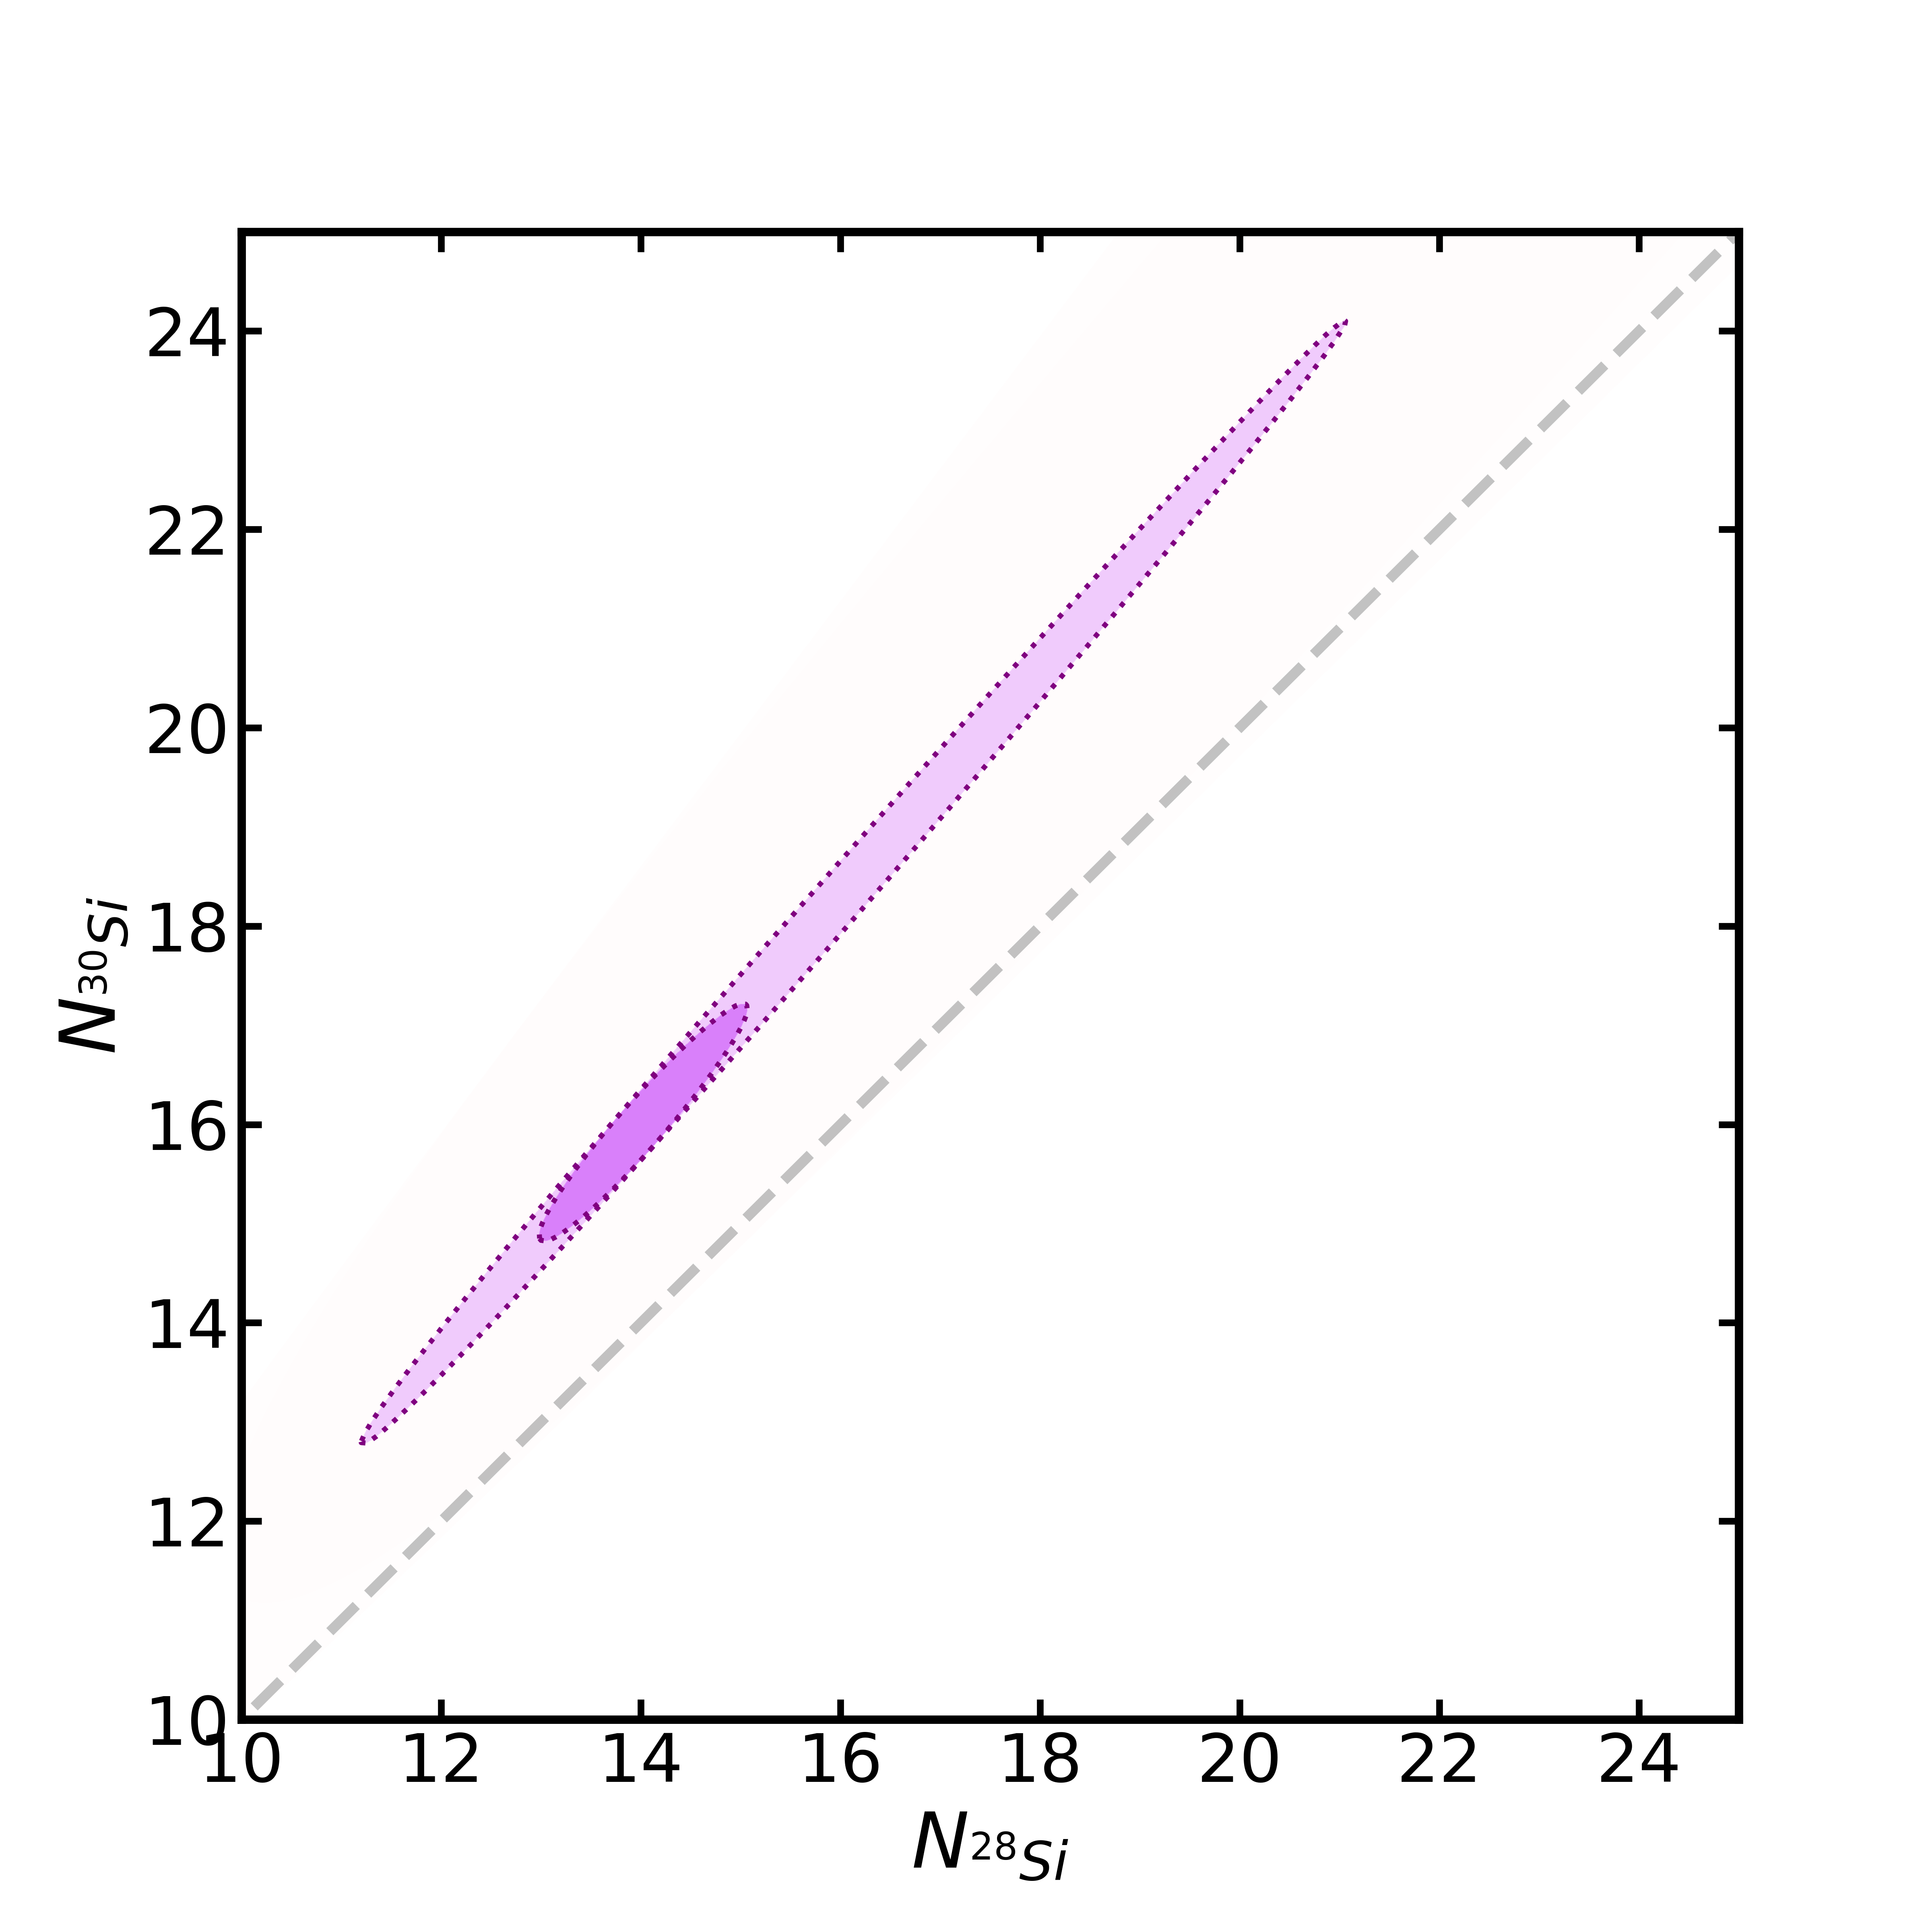
\includegraphics[scale=0.35]{figures/N2Si1.png}}\hspace{-1em}%
\subfigure[\emph{2 - 3 KeV}]{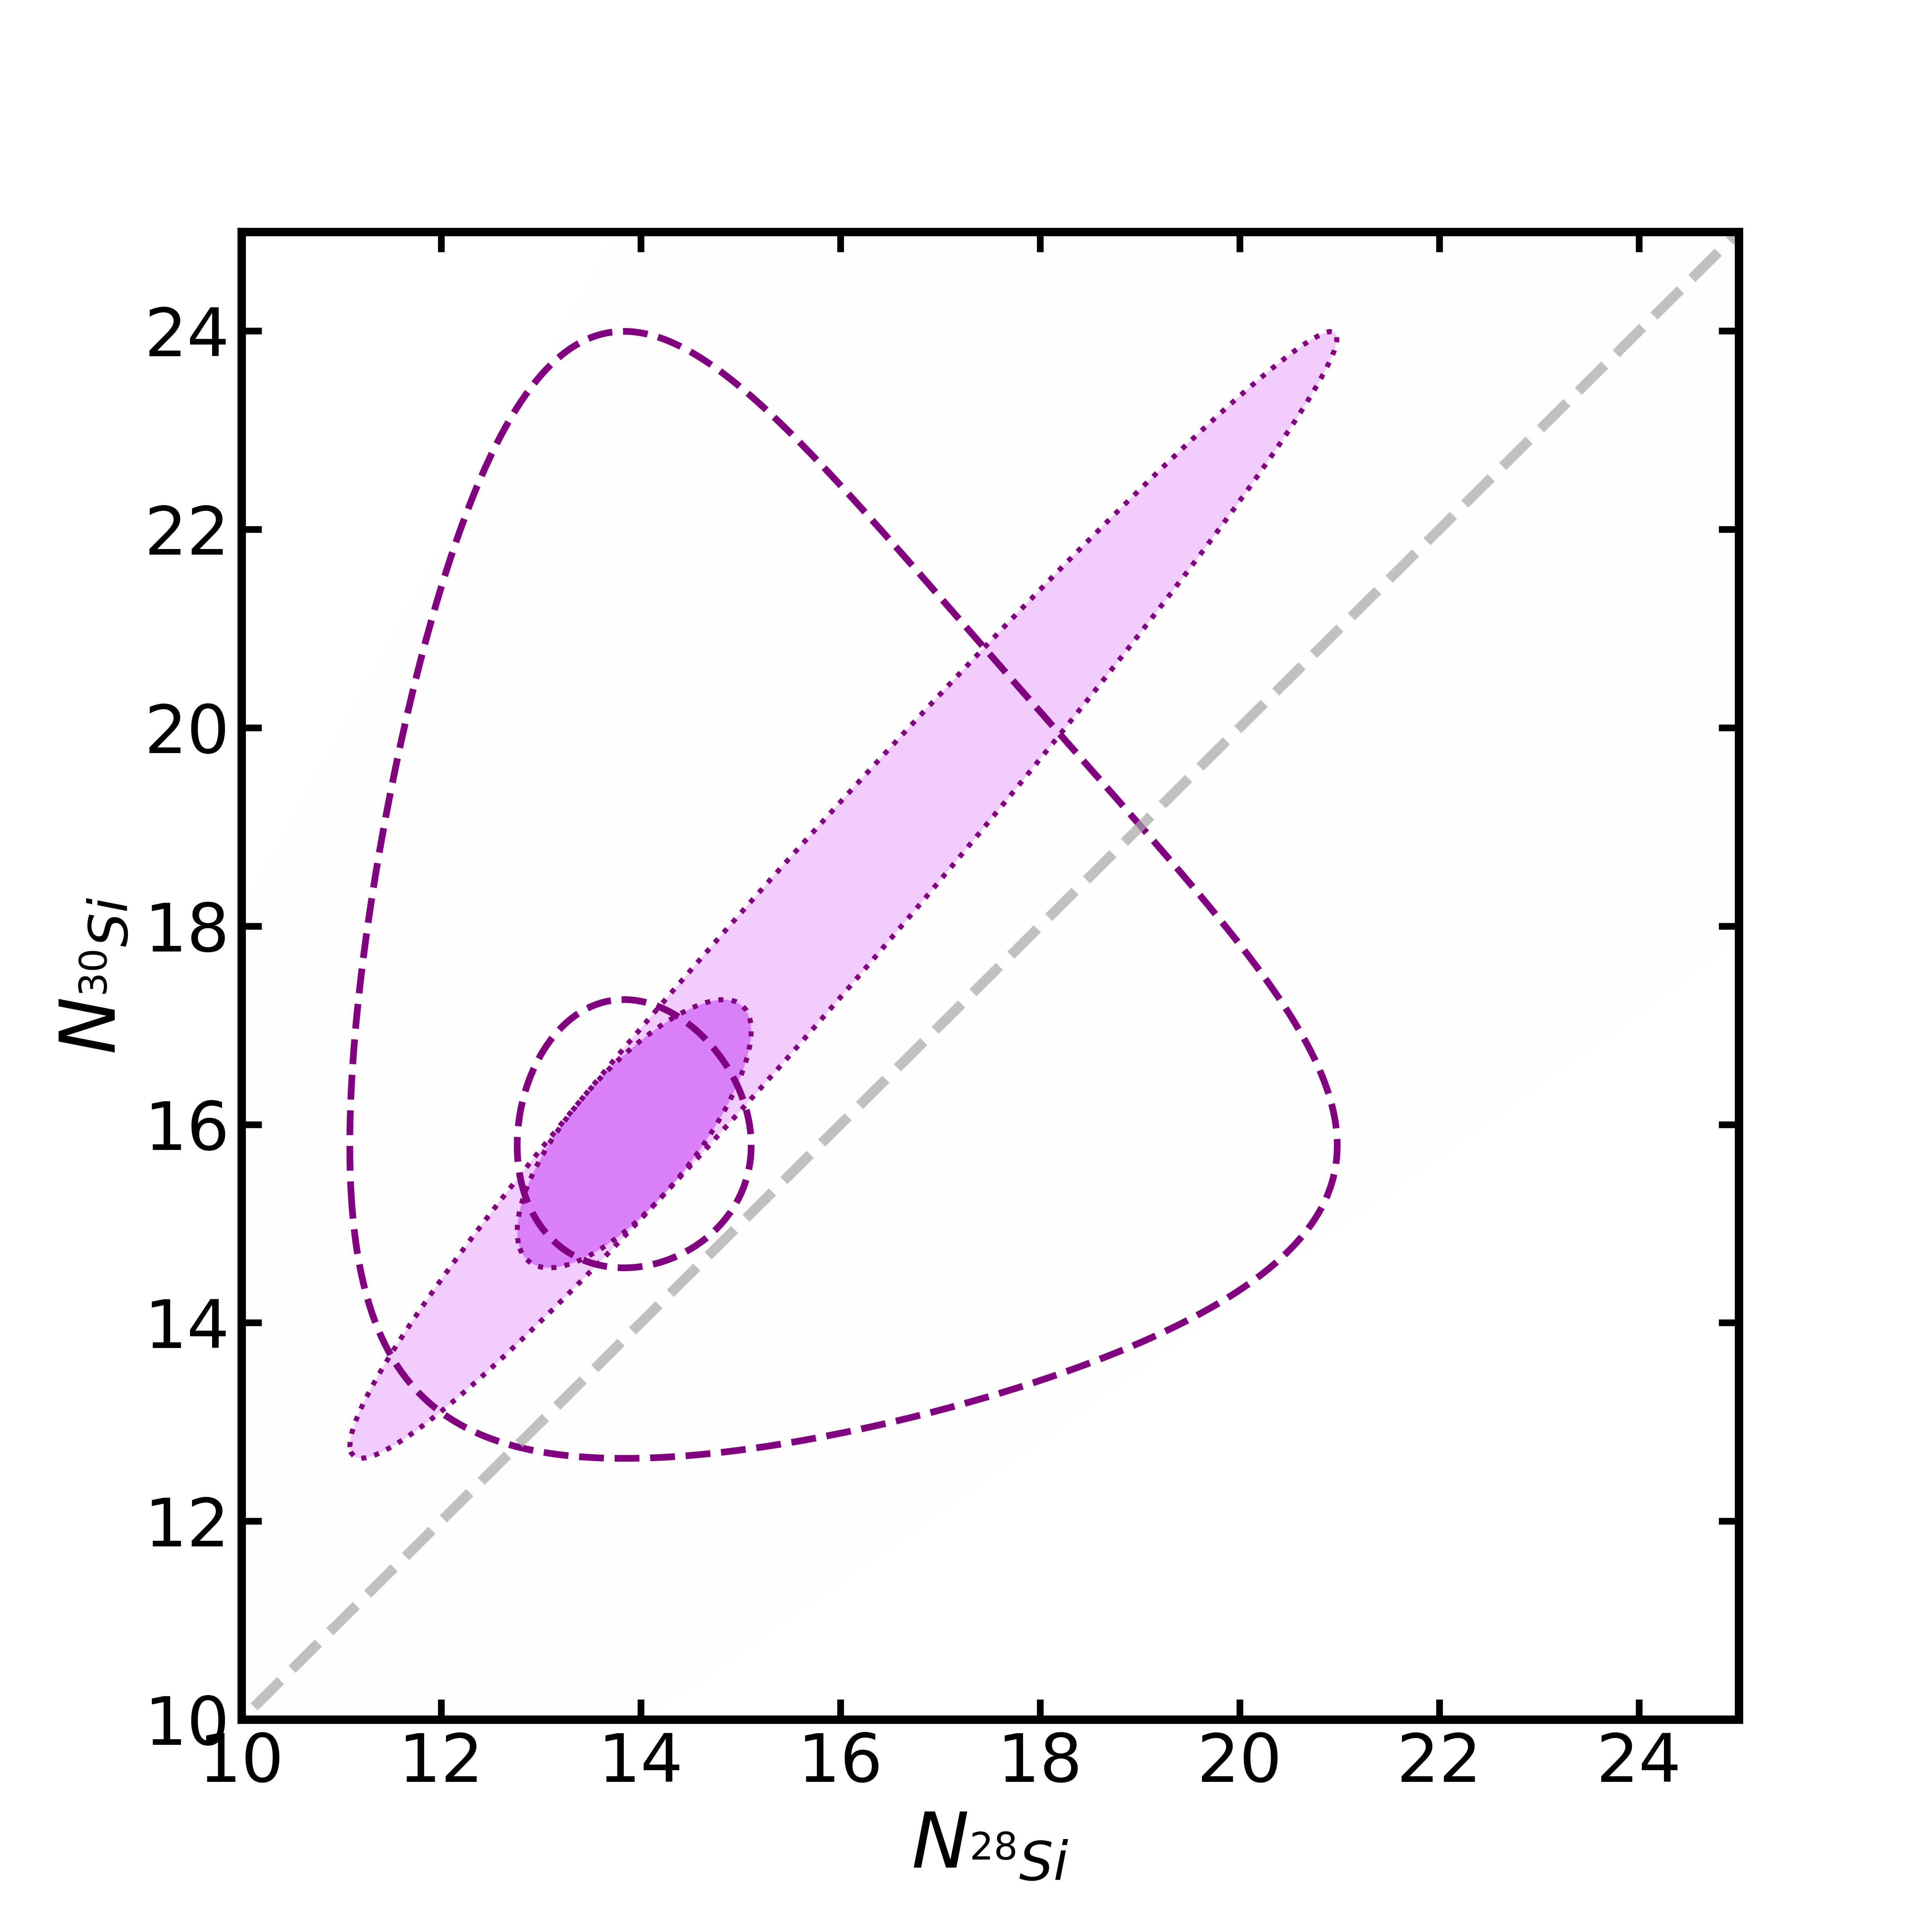
\includegraphics[scale=0.35]{figures/N2SiNC.png}}
     \caption{Expected allowed values of the N' factor at a 90$\%$ confidence level for Si isotopes detector exposed to reactor antineutrino flux with different ranges of recoil energy. Light regions refer to the case of $\sigma_A = 25\%$ and $\sigma_B=10\%$ while dark regions refer to the case of $\sigma_A=\sigma_B=5\%$. In (a), the uncorrelated case is also shown in dashed lines.}
     \label{SiReactor}
\end{figure}
 Now, we aim to investigate whether a counting experiment of this nature would yield a number of events that is consistent with the quadratic dependence on the number of neutrons of the CEvNS cross-section.\\
 To corroborate this, we will obtain the regions where the permissible values of the expected number of events are evident instead of the number of neutrons. This is presented in figure \ref{N2EventsZn} for Zinc. For this analysis, we utilize the flux from the reactor, which provides the advantage of having a substantial amount of statistical data.
 Different recoil energy ranges are being examined. This is because it is understood that the event count will fluctuate based on the specific range chosen.\\
 In the recoil energy interval of 1-2 KeV, we are situated above the intersection point shown in figure \ref{fig8}. Here, we have reached the kinematic limit, which causes the lighter isotope to exhibit a higher number of events than the heavier one. This is evident in figure \ref{N2EventsZn} (a). In this recoil energy region, the quadratic dependence of N is not satisfied. We find ourselves precisely at the crossover region in the 0.7-1 KeV energy range in panel (b) of the figure mentioned above, where it is evident that we have approximately the same number of events for both isotopes. Finally, in panel (c) of the figure, the 0.4-0.7 KeV energy range is analyzed. This zone is located below the crossover point and, indeed, here the heavier isotope exhibits a higher number of events, confirming the dependence of $N^2$.
\begin{figure}[h!]
\centering
\subfigure[\emph{1 - 2 KeV}]{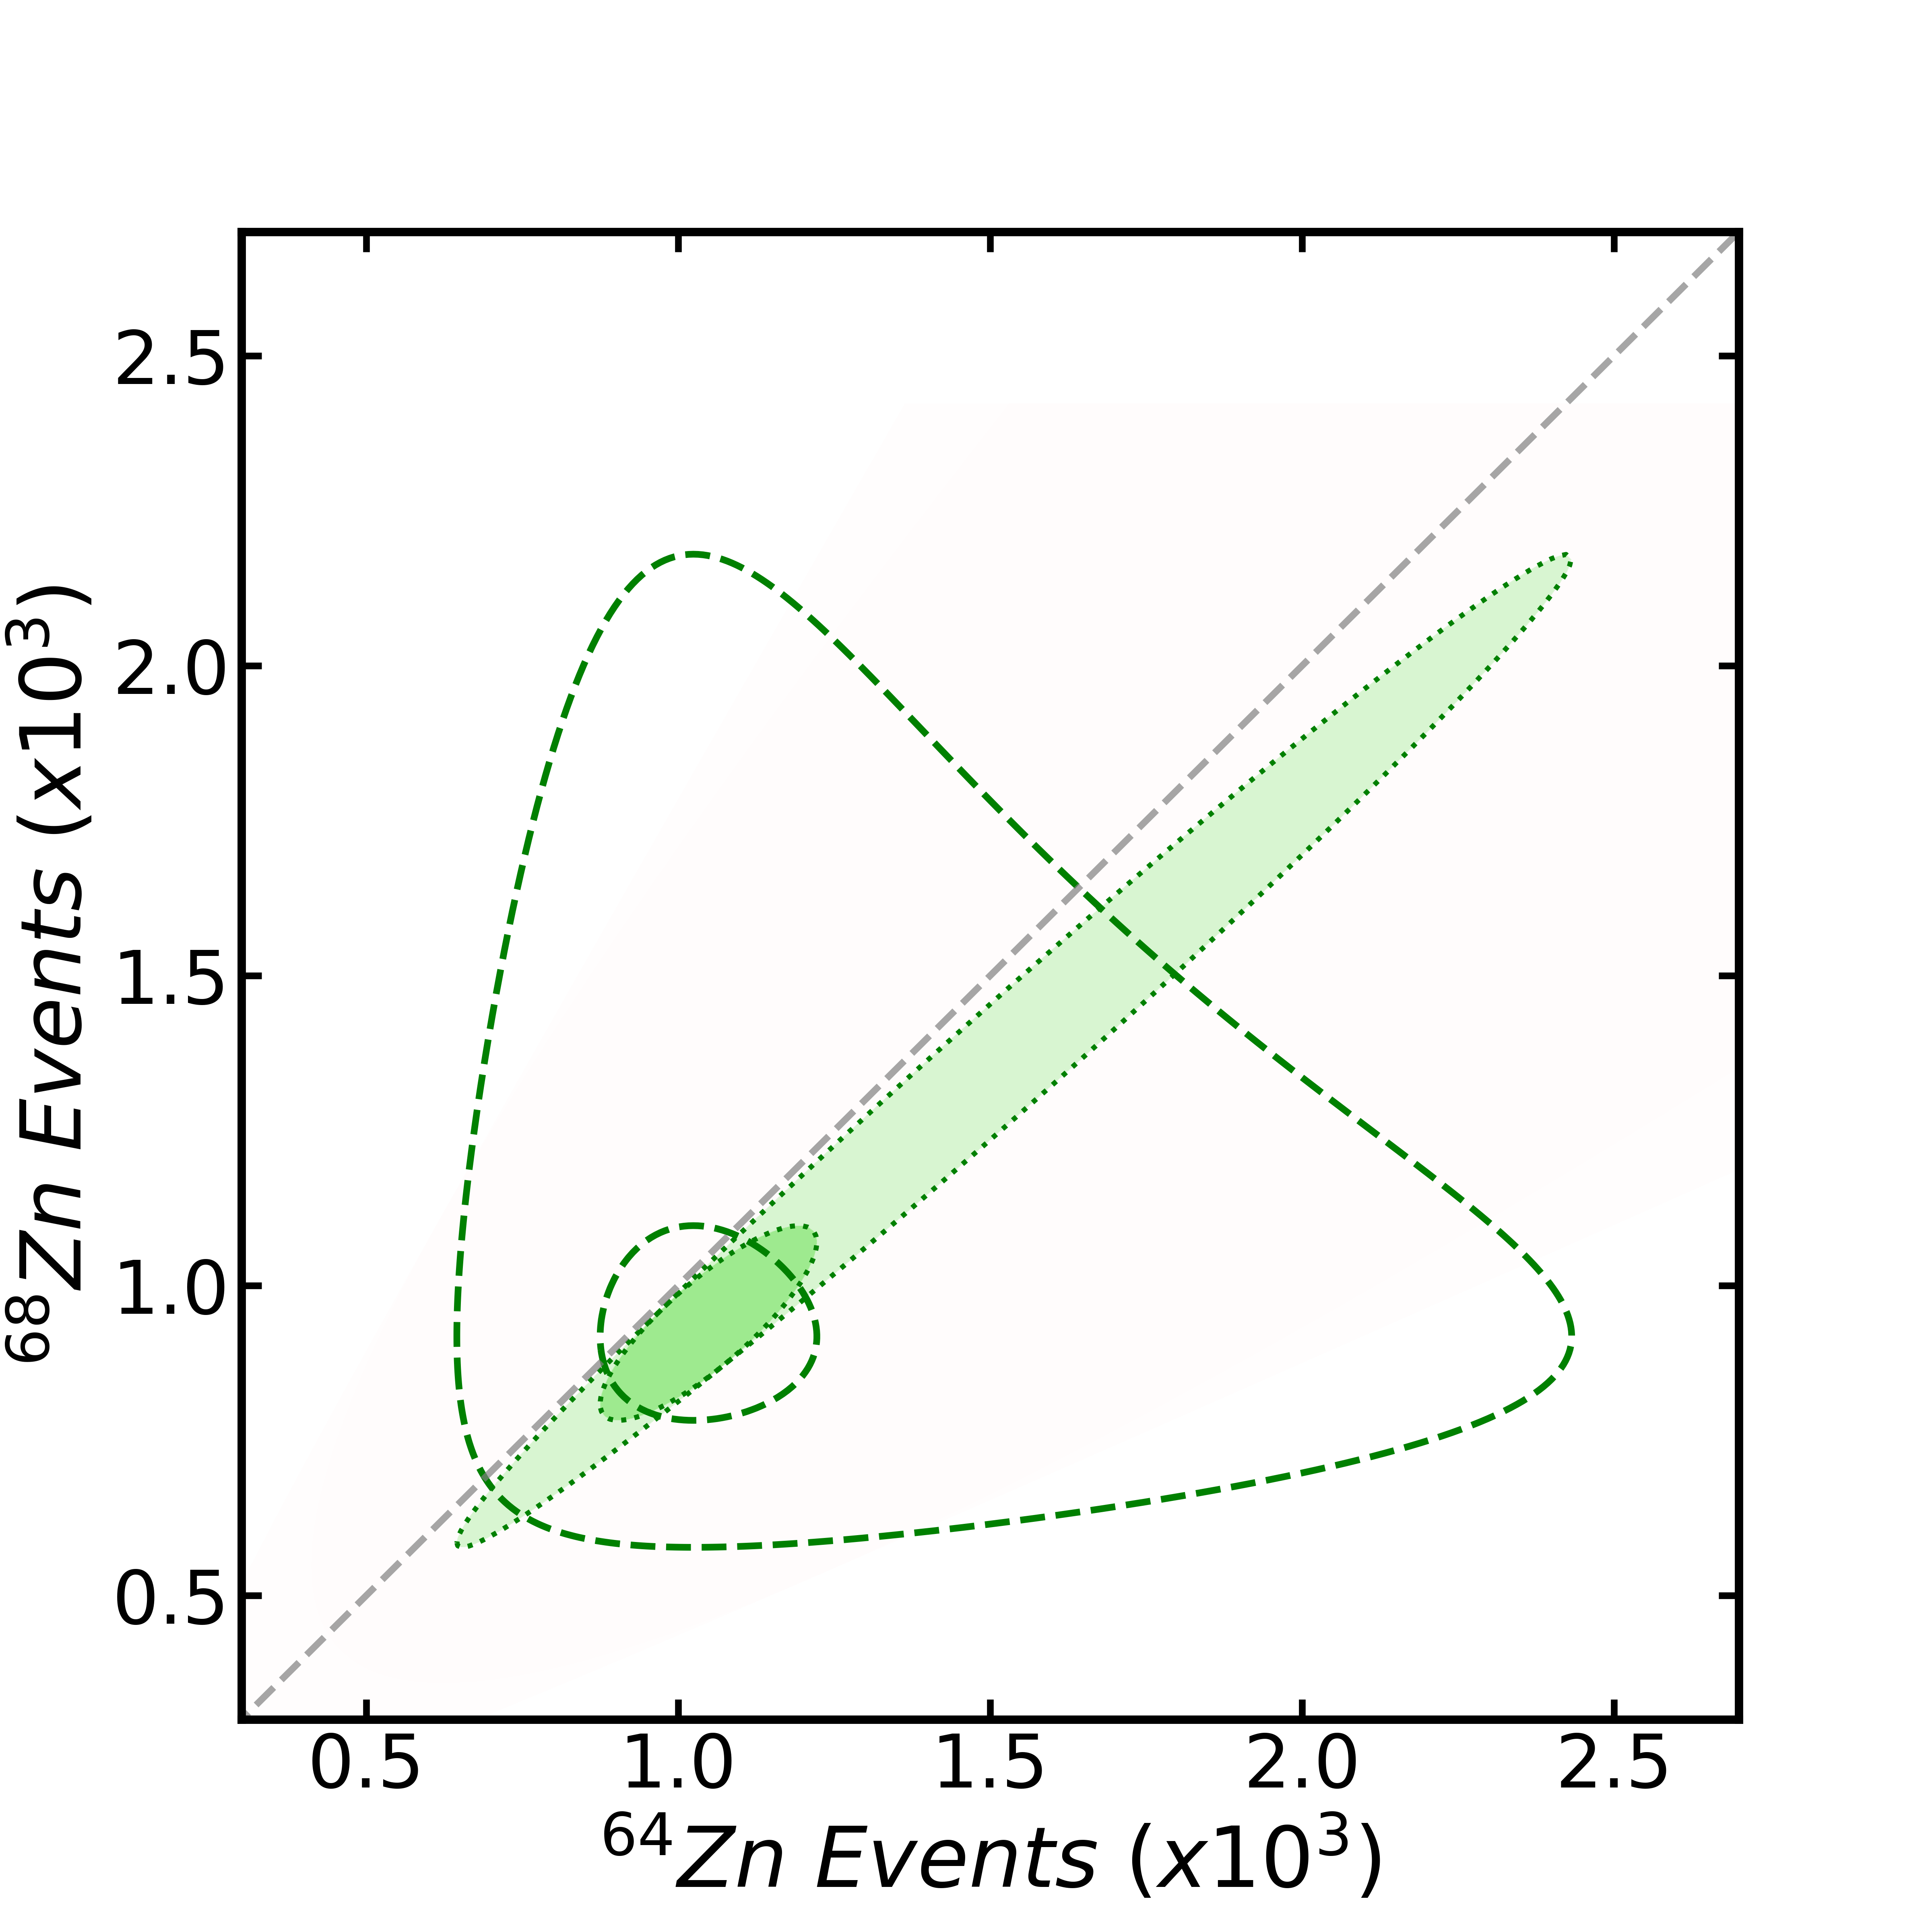
\includegraphics[scale=0.33]{figures/N2ZnEventsNC.png}}\hspace{-1em}%
\subfigure[\emph{0.7 - 1 KeV}]{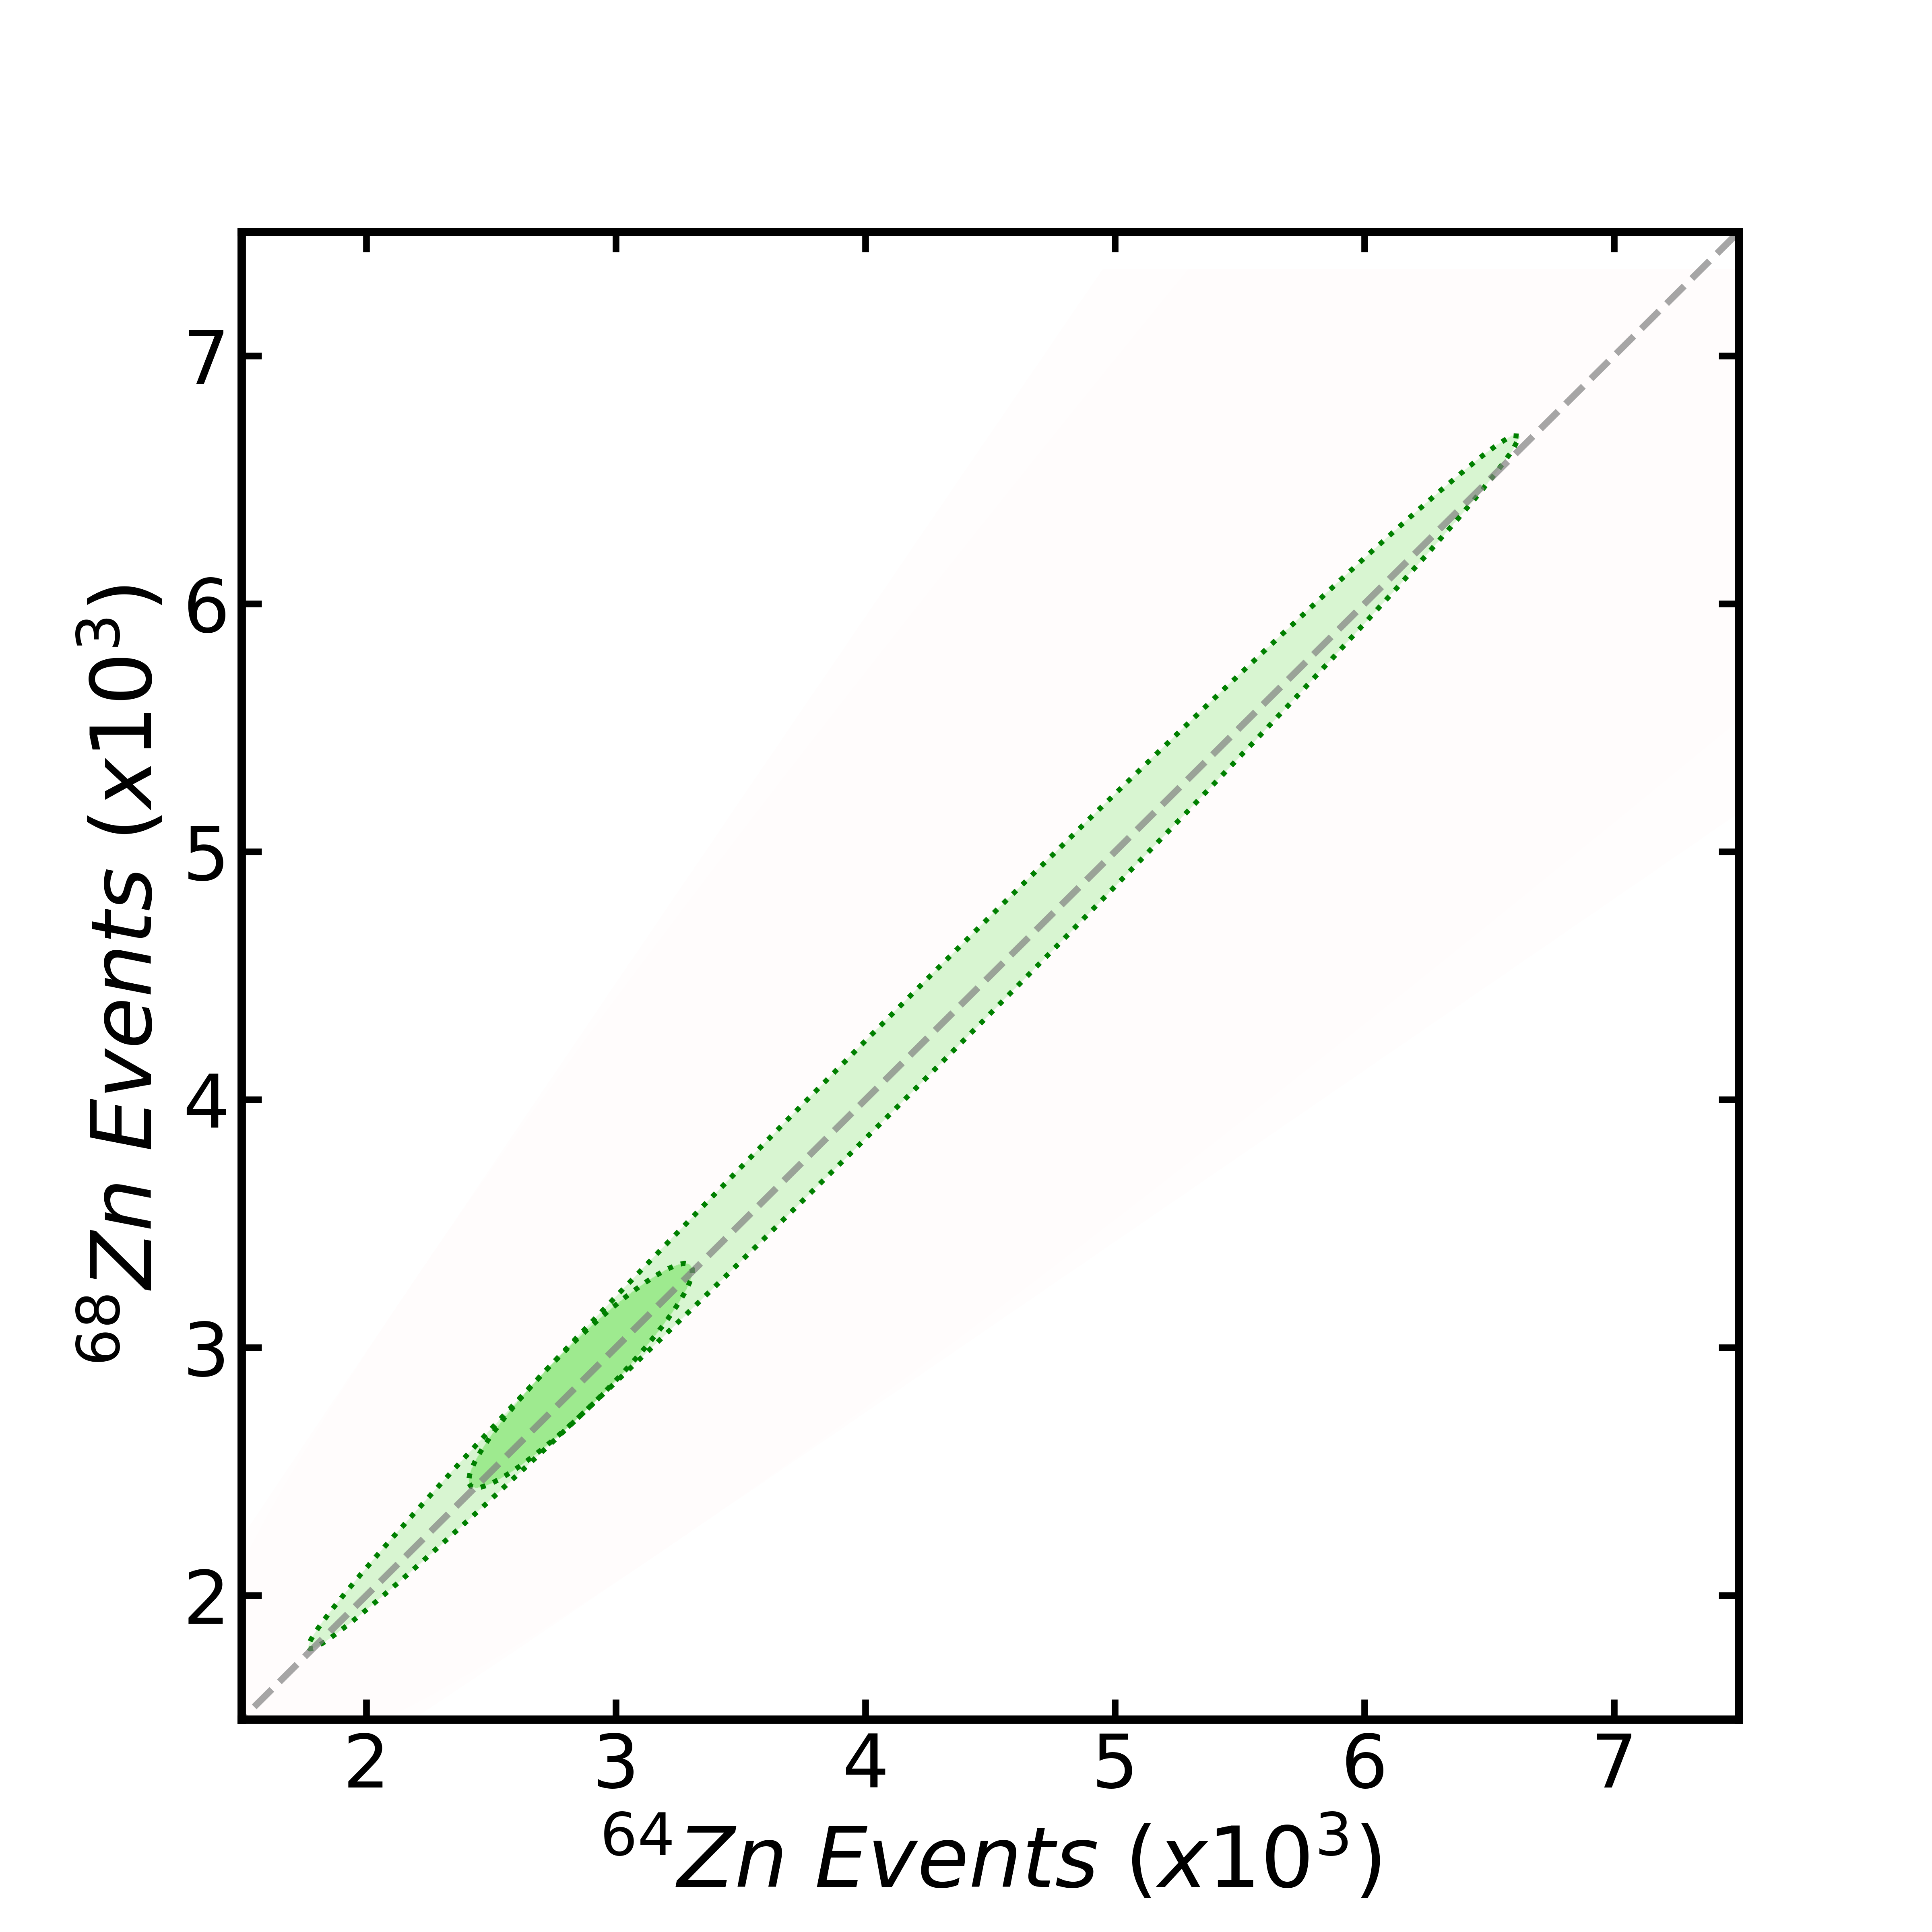
\includegraphics[scale=0.33]{figures/N2ZnEvents7-2.png}}\par \vspace{-1em}%
\subfigure[\emph{0.4 - 0.7 KeV}]{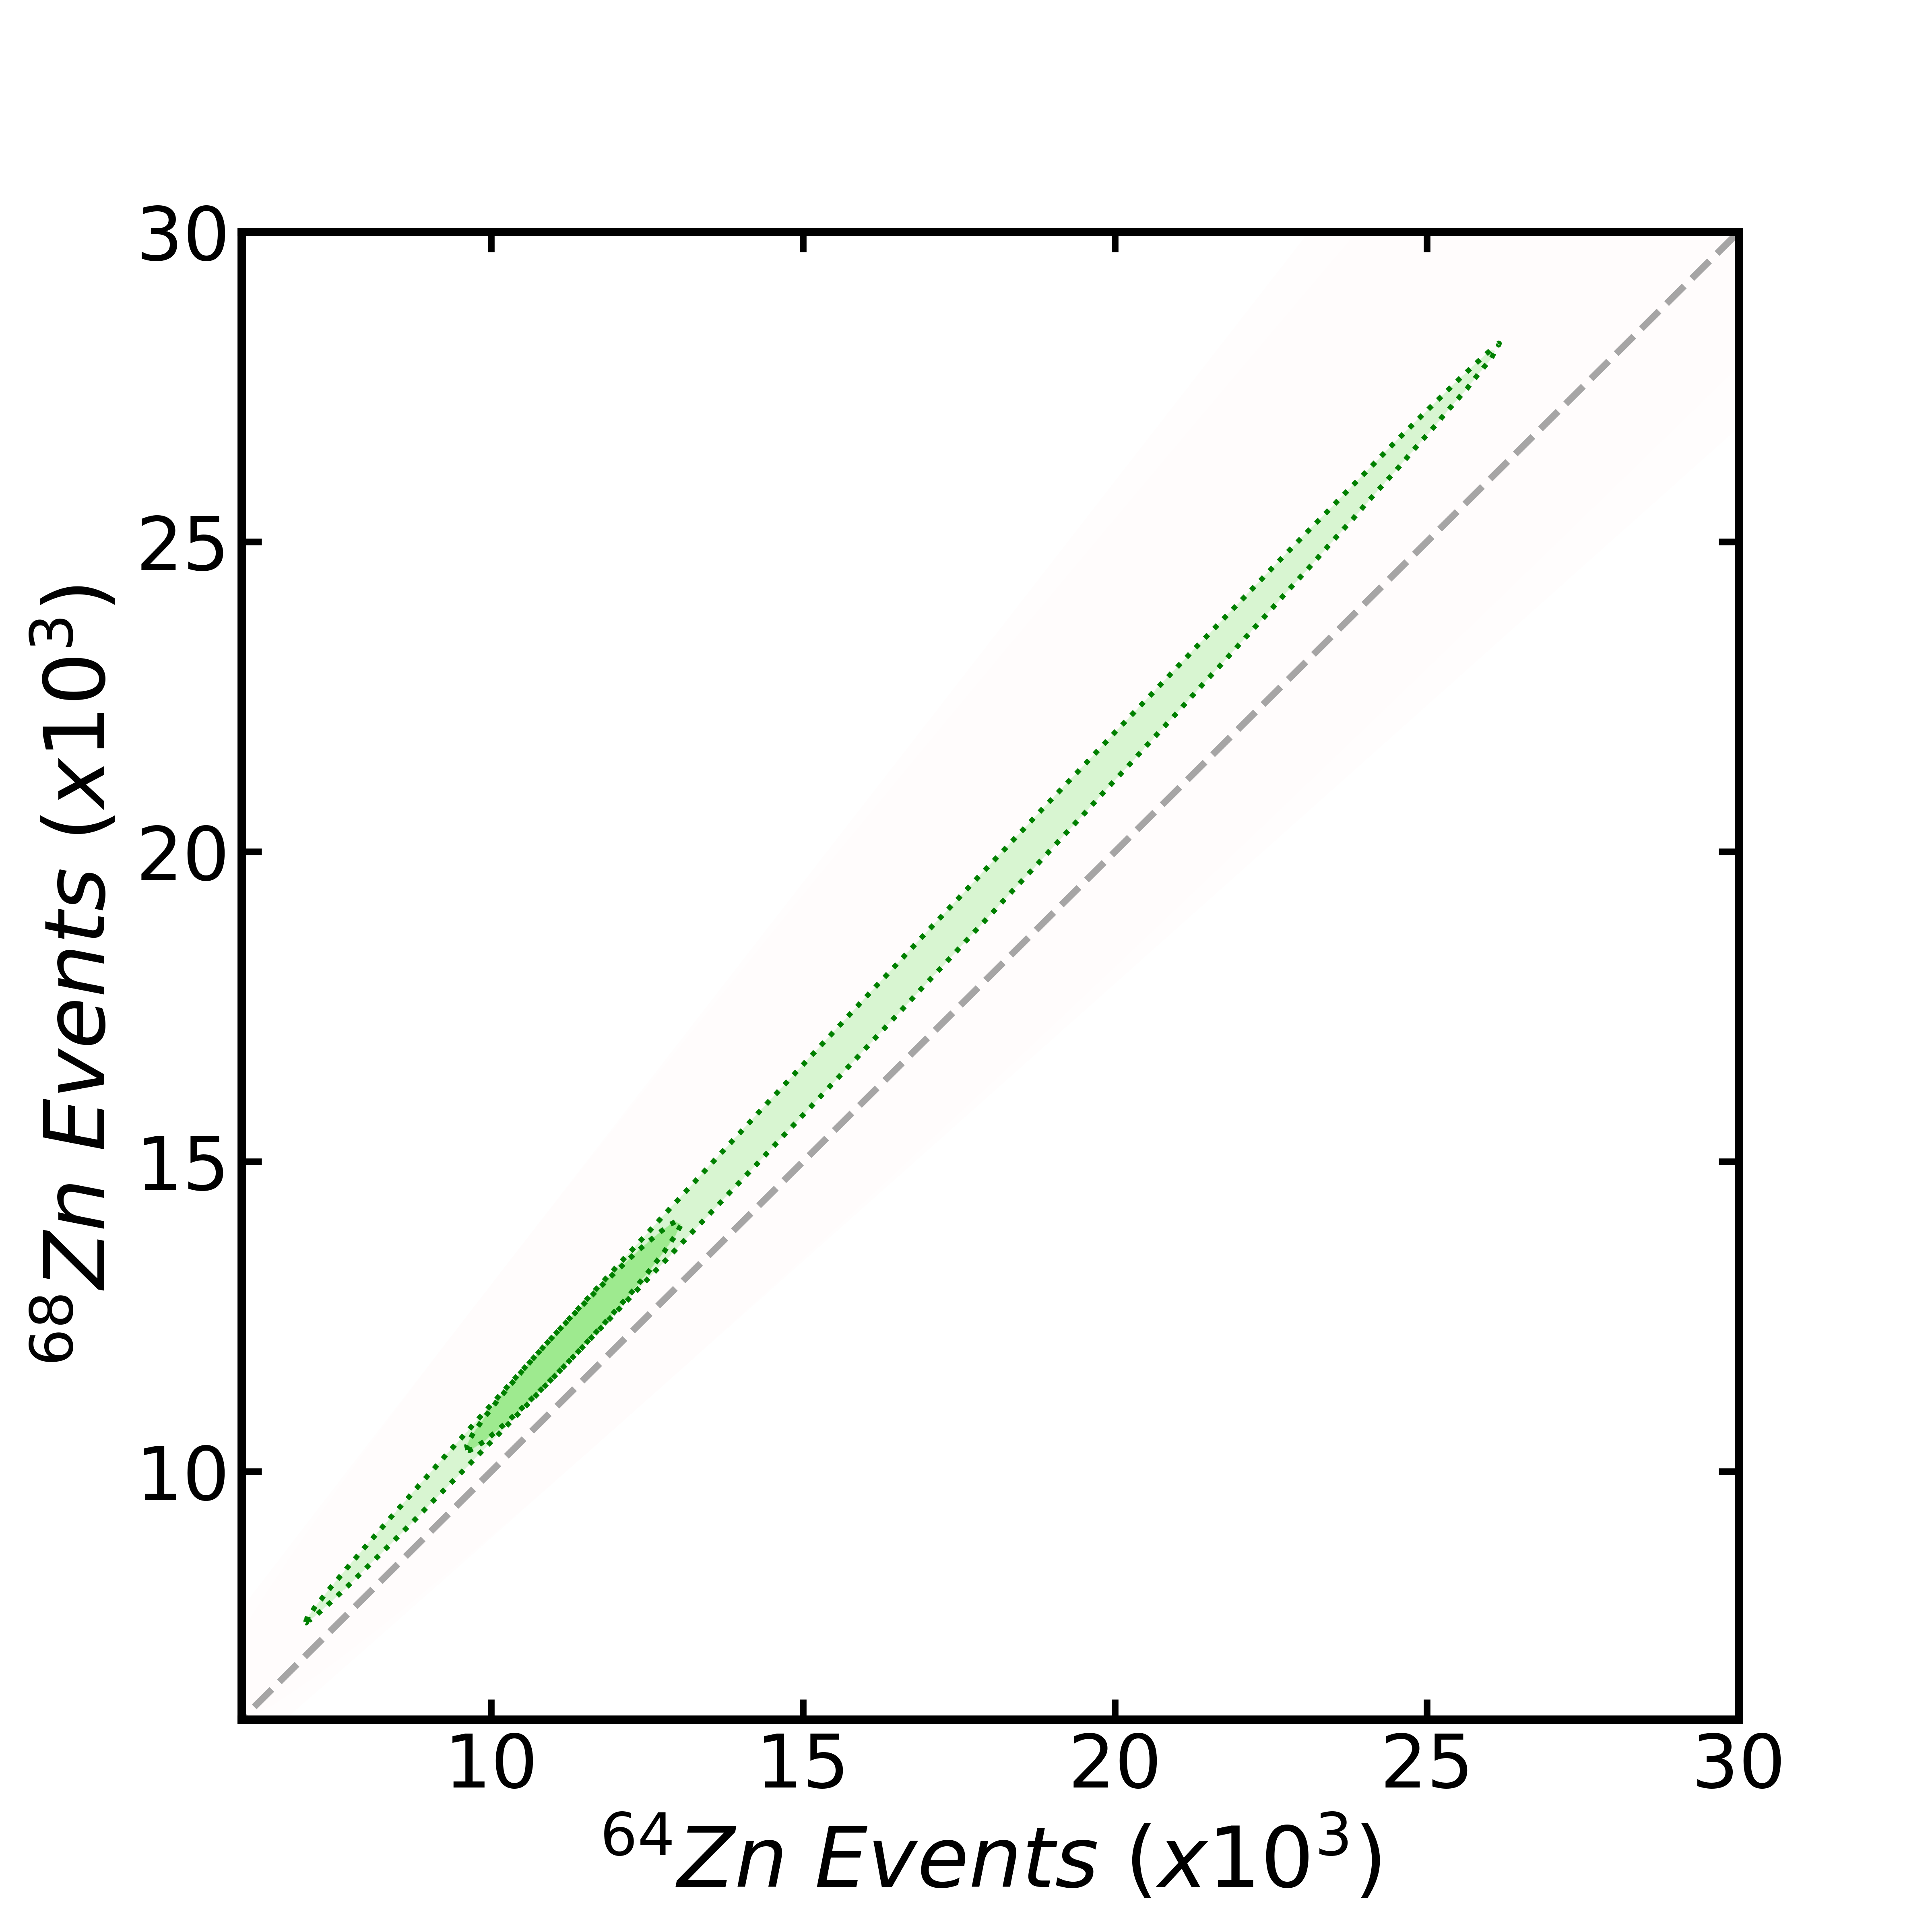
\includegraphics[scale=0.33]{figures/N2ZnEvents4-2.png}}
\caption{Expected number of events for Zn isotopes detector exposed to reactor antineutrino flux with different ranges of recoil energy. Light regions refer to the case of $\sigma_A = 25\%$ and $\sigma_B=10\%$ while dark regions refer to the case of $\sigma_A=\sigma_B=5\%$.In (a), the uncorrelated case is also shown in dashed lines.}
\label{N2EventsZn}
\end{figure}

This same analysis is carried out for the Silicon isotopes, as shown in figure \ref{N2EventsSi}. For this material, we consider four recoil energy regions. This is because its crossover point in figure \ref{fig8} occurs at higher energies than the zin case. Therefore, including the interval 2-3 KeV allows for a more accurate comparison between the materials. 

\begin{figure}[h!]
\centering
\subfigure[\emph{2 - 3 KeV}]{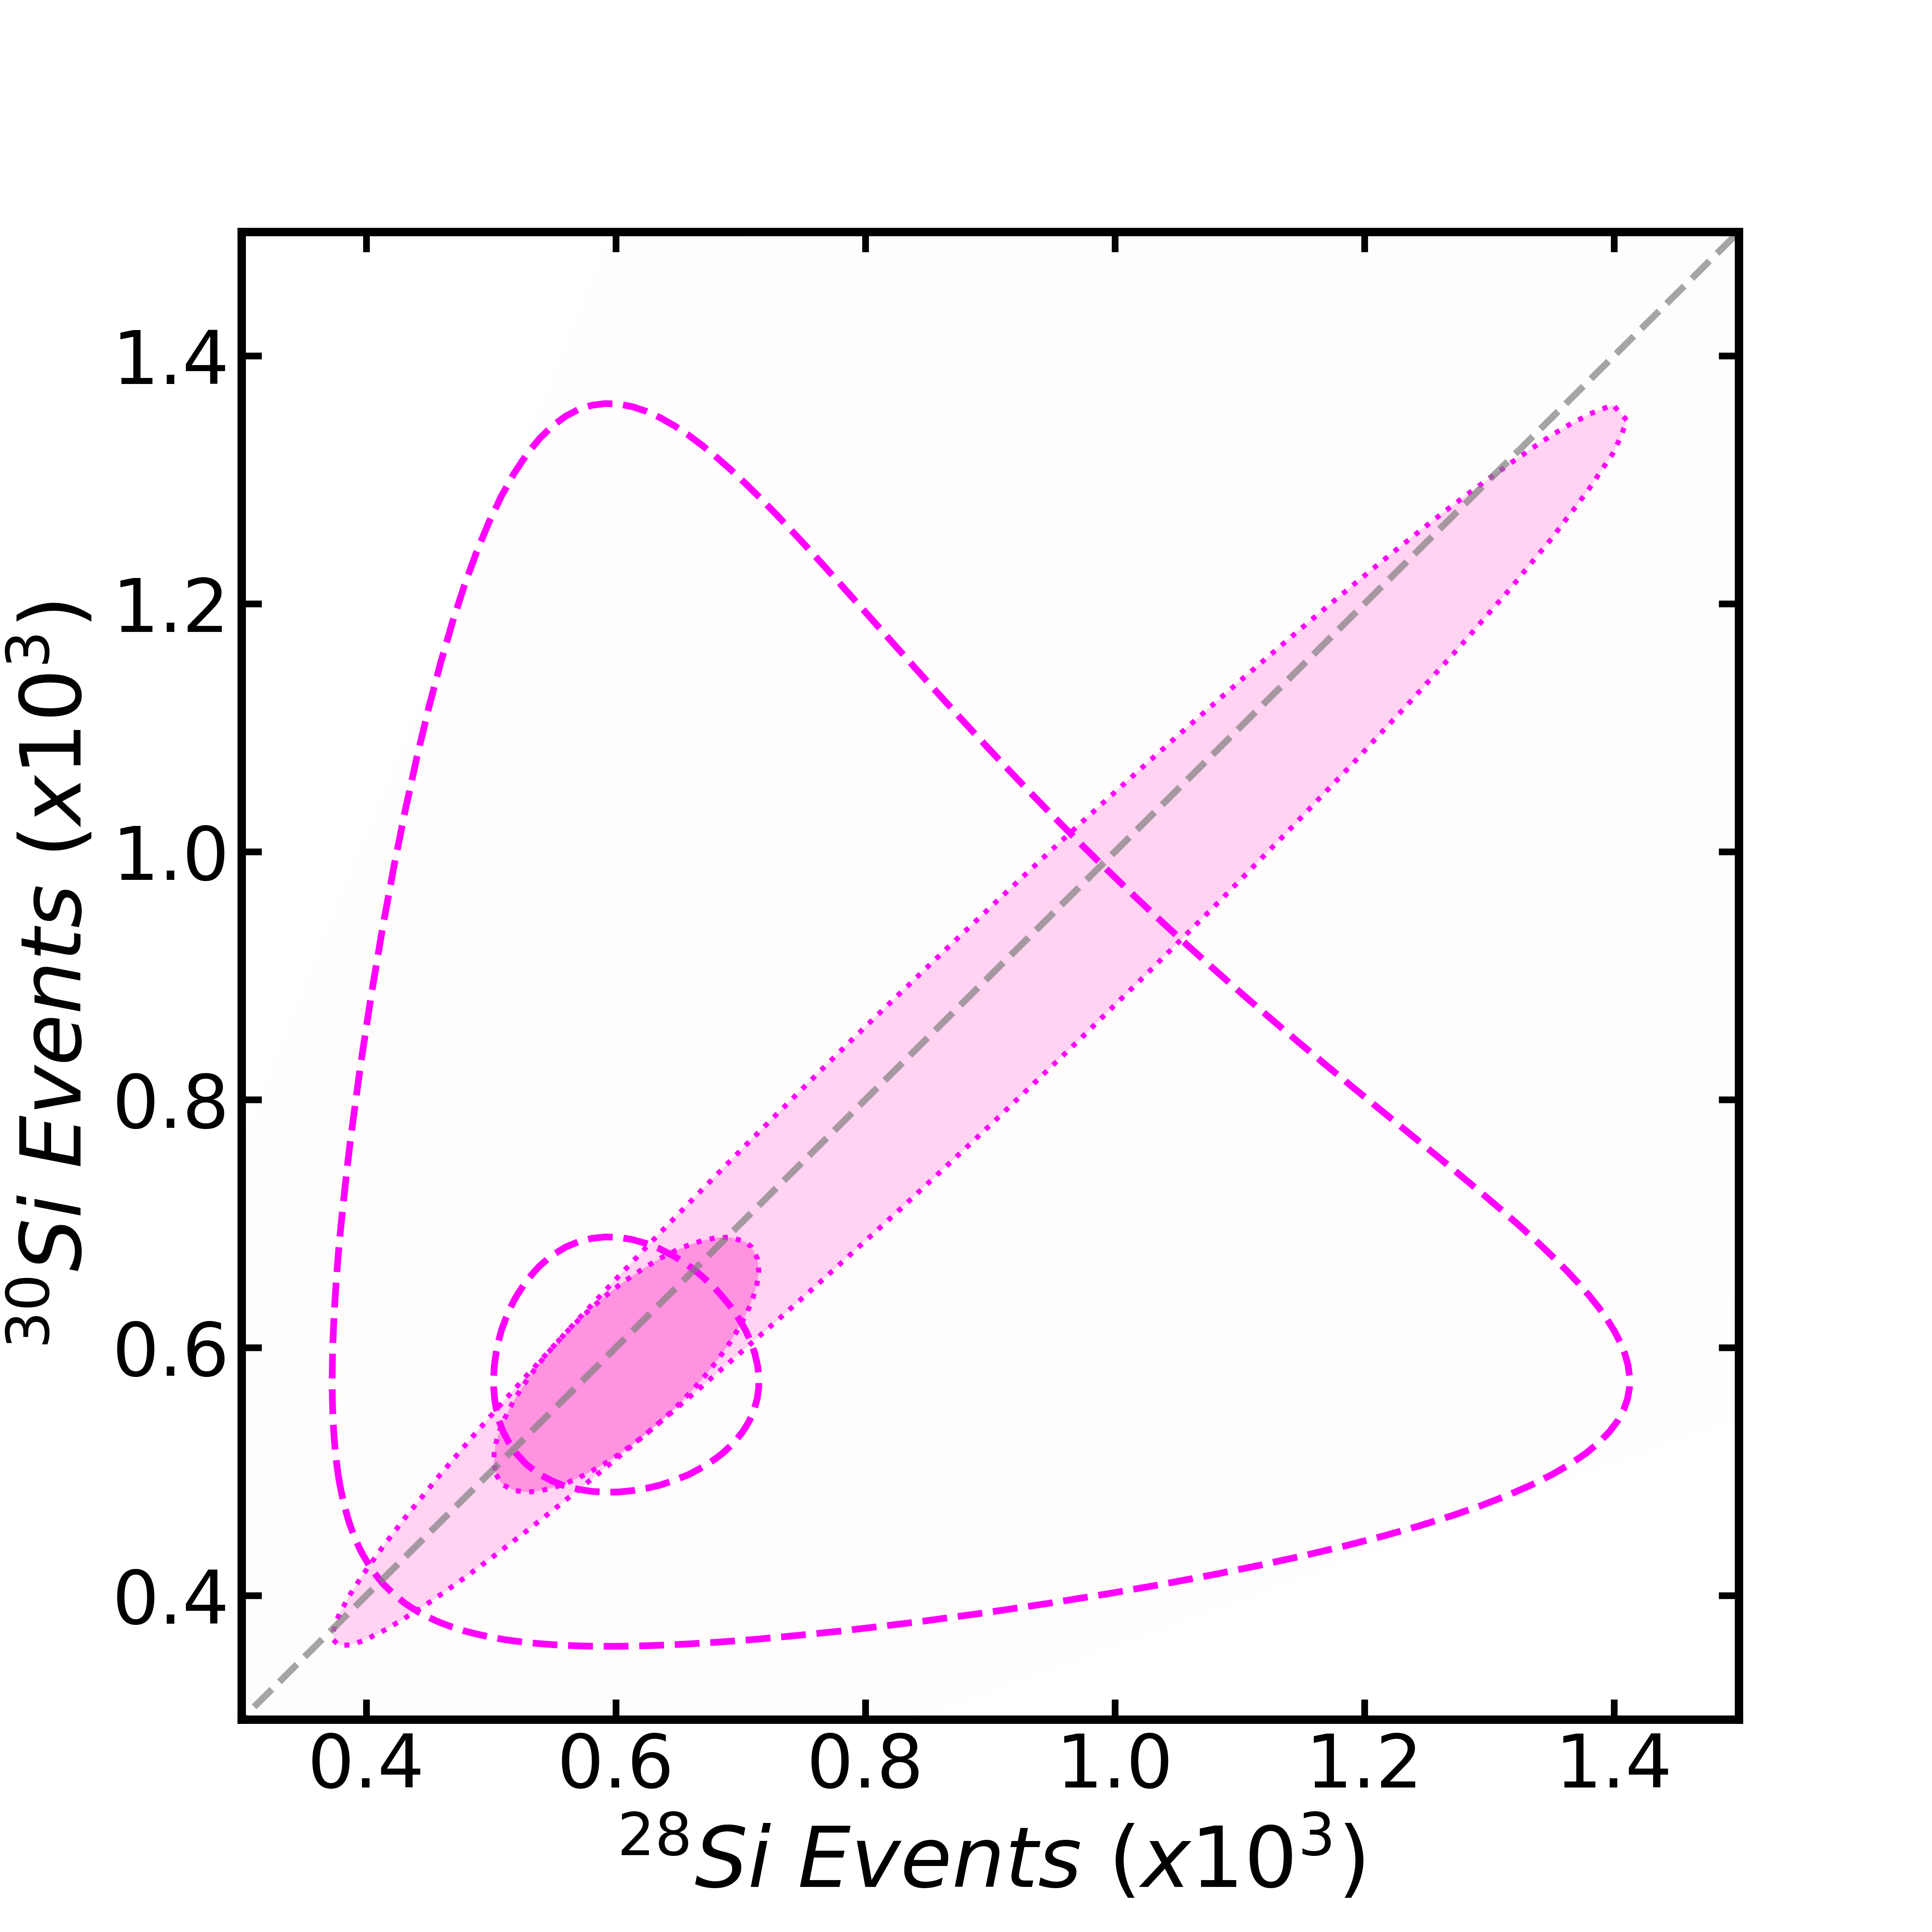
\includegraphics[scale=0.33]{figures/N2SiEventsNC.png}}\hspace{-1em}%
\subfigure[\emph{1 - 2 KeV}]{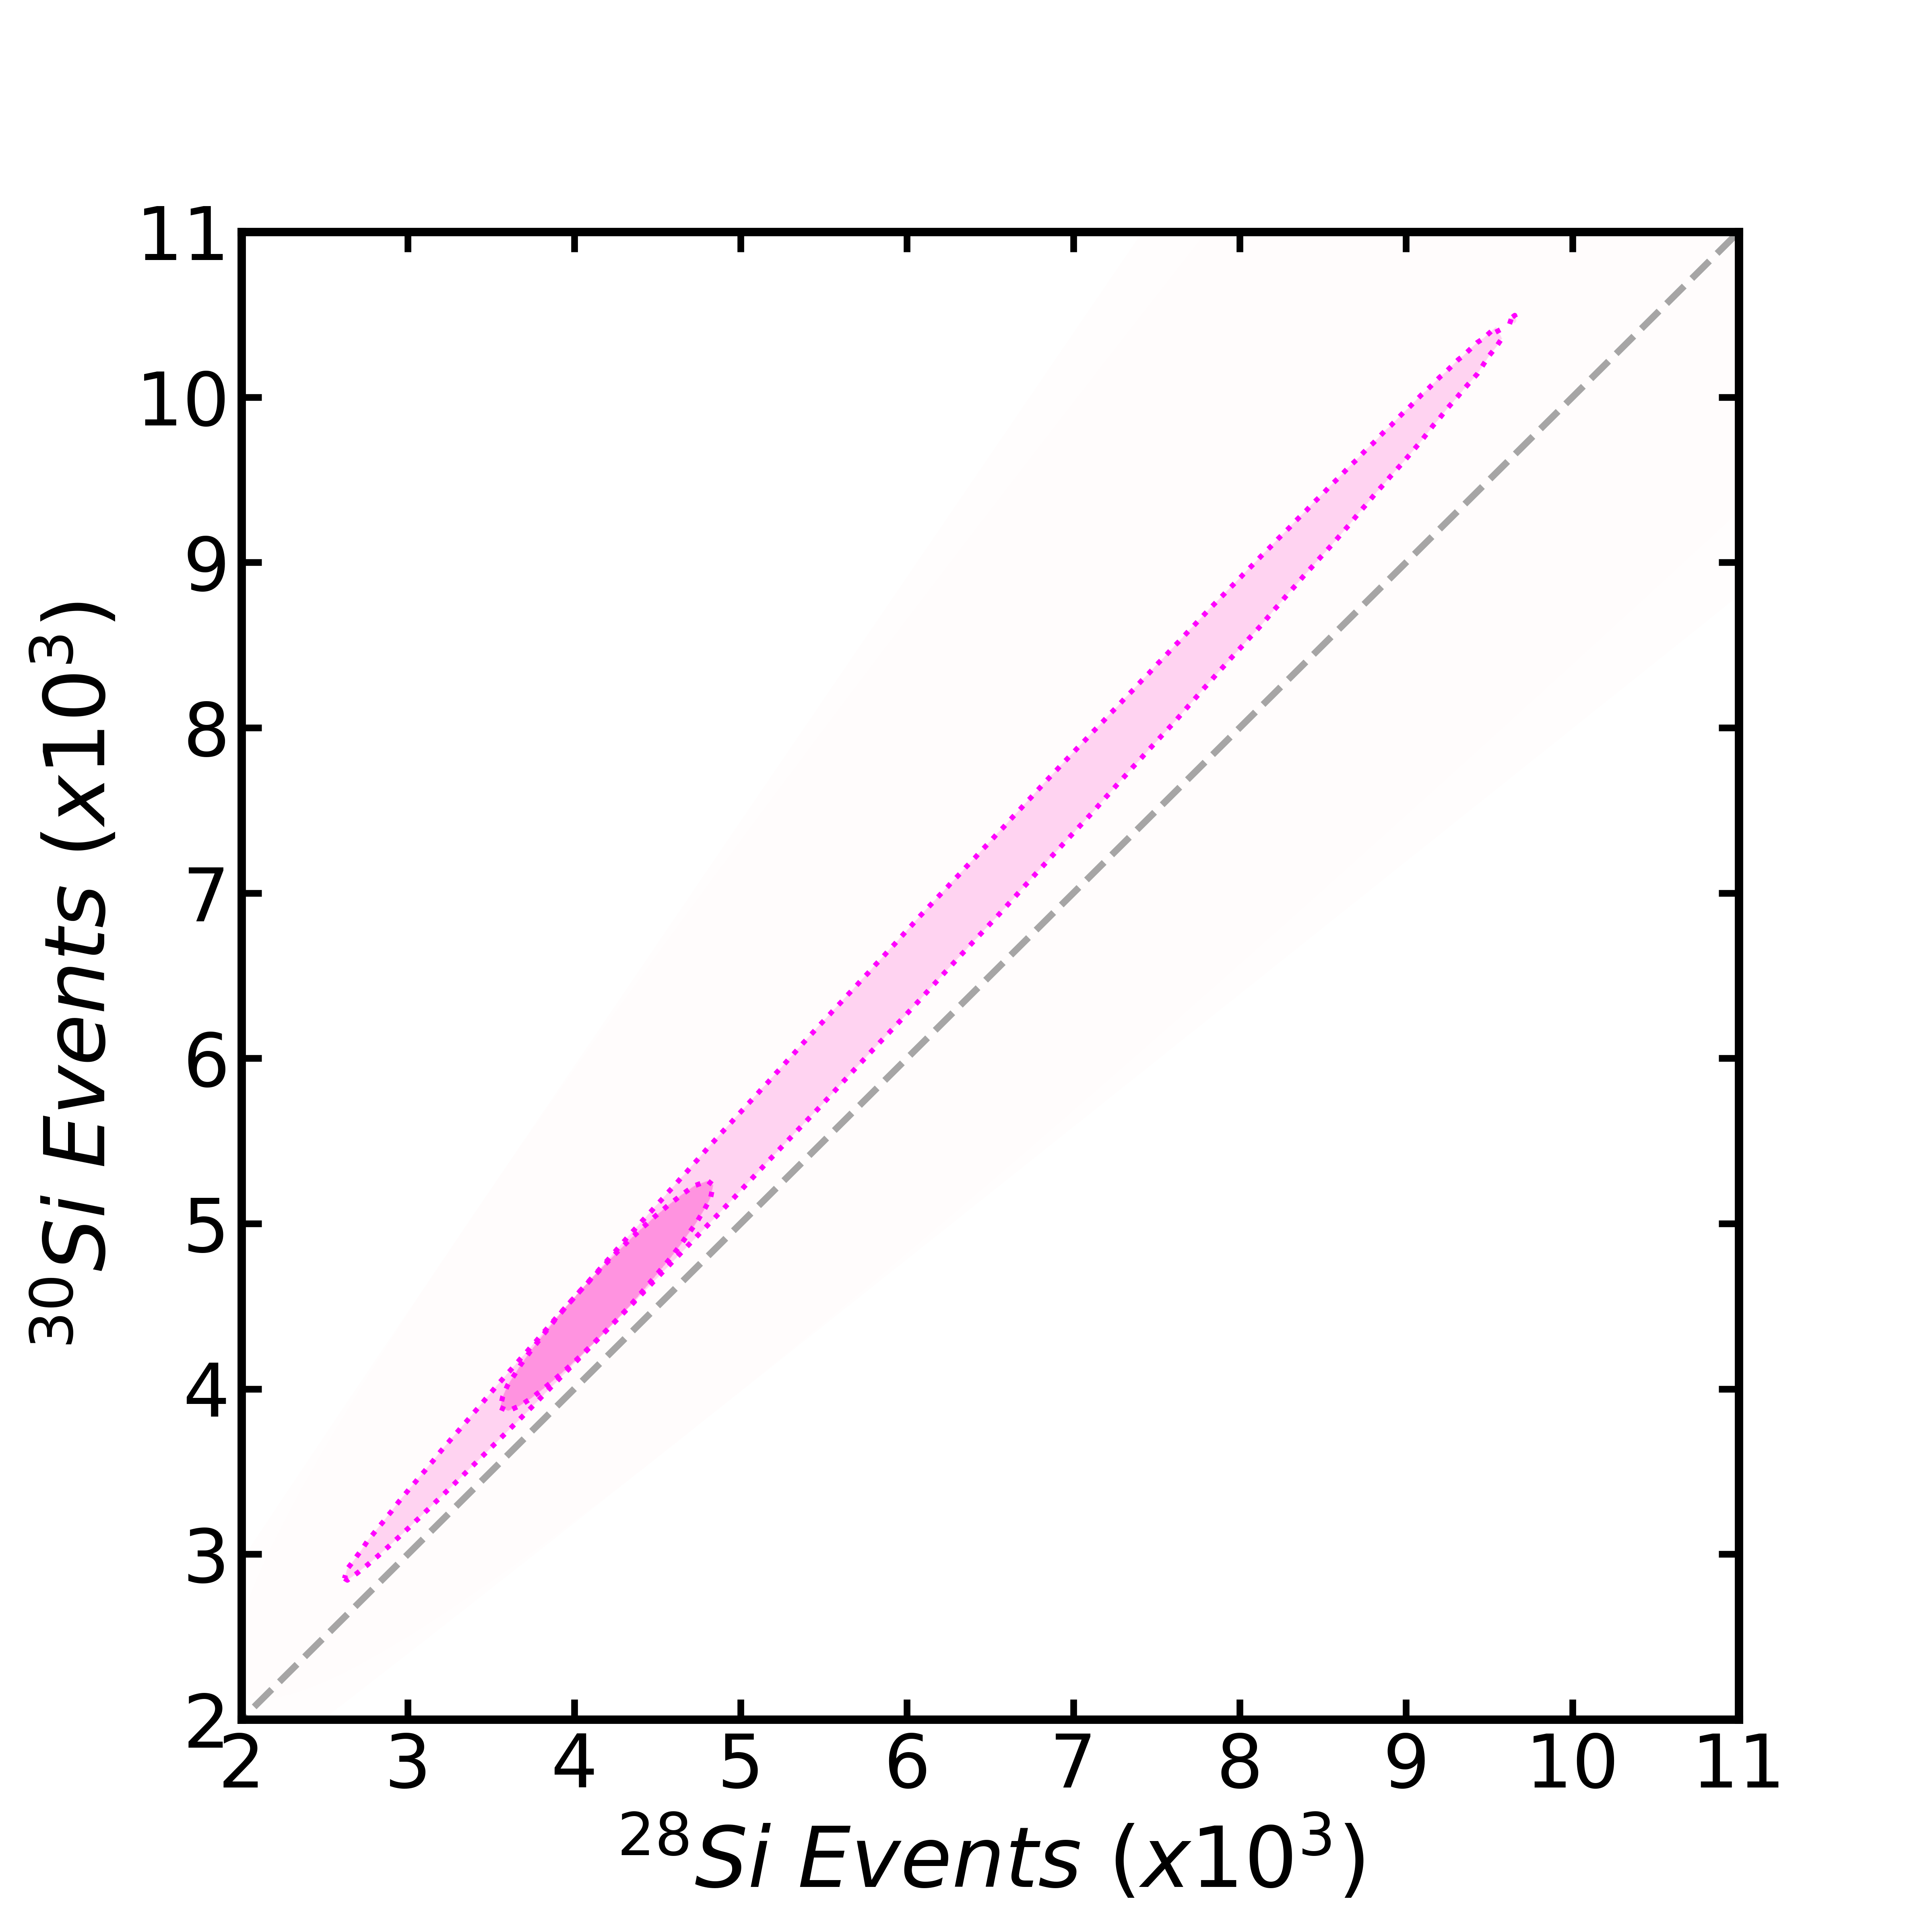
\includegraphics[scale=0.33]{figures/N2SiEvents1-2.png}}\par \vspace{-1em}%
\subfigure[\emph{0.7 - 1 KeV}]{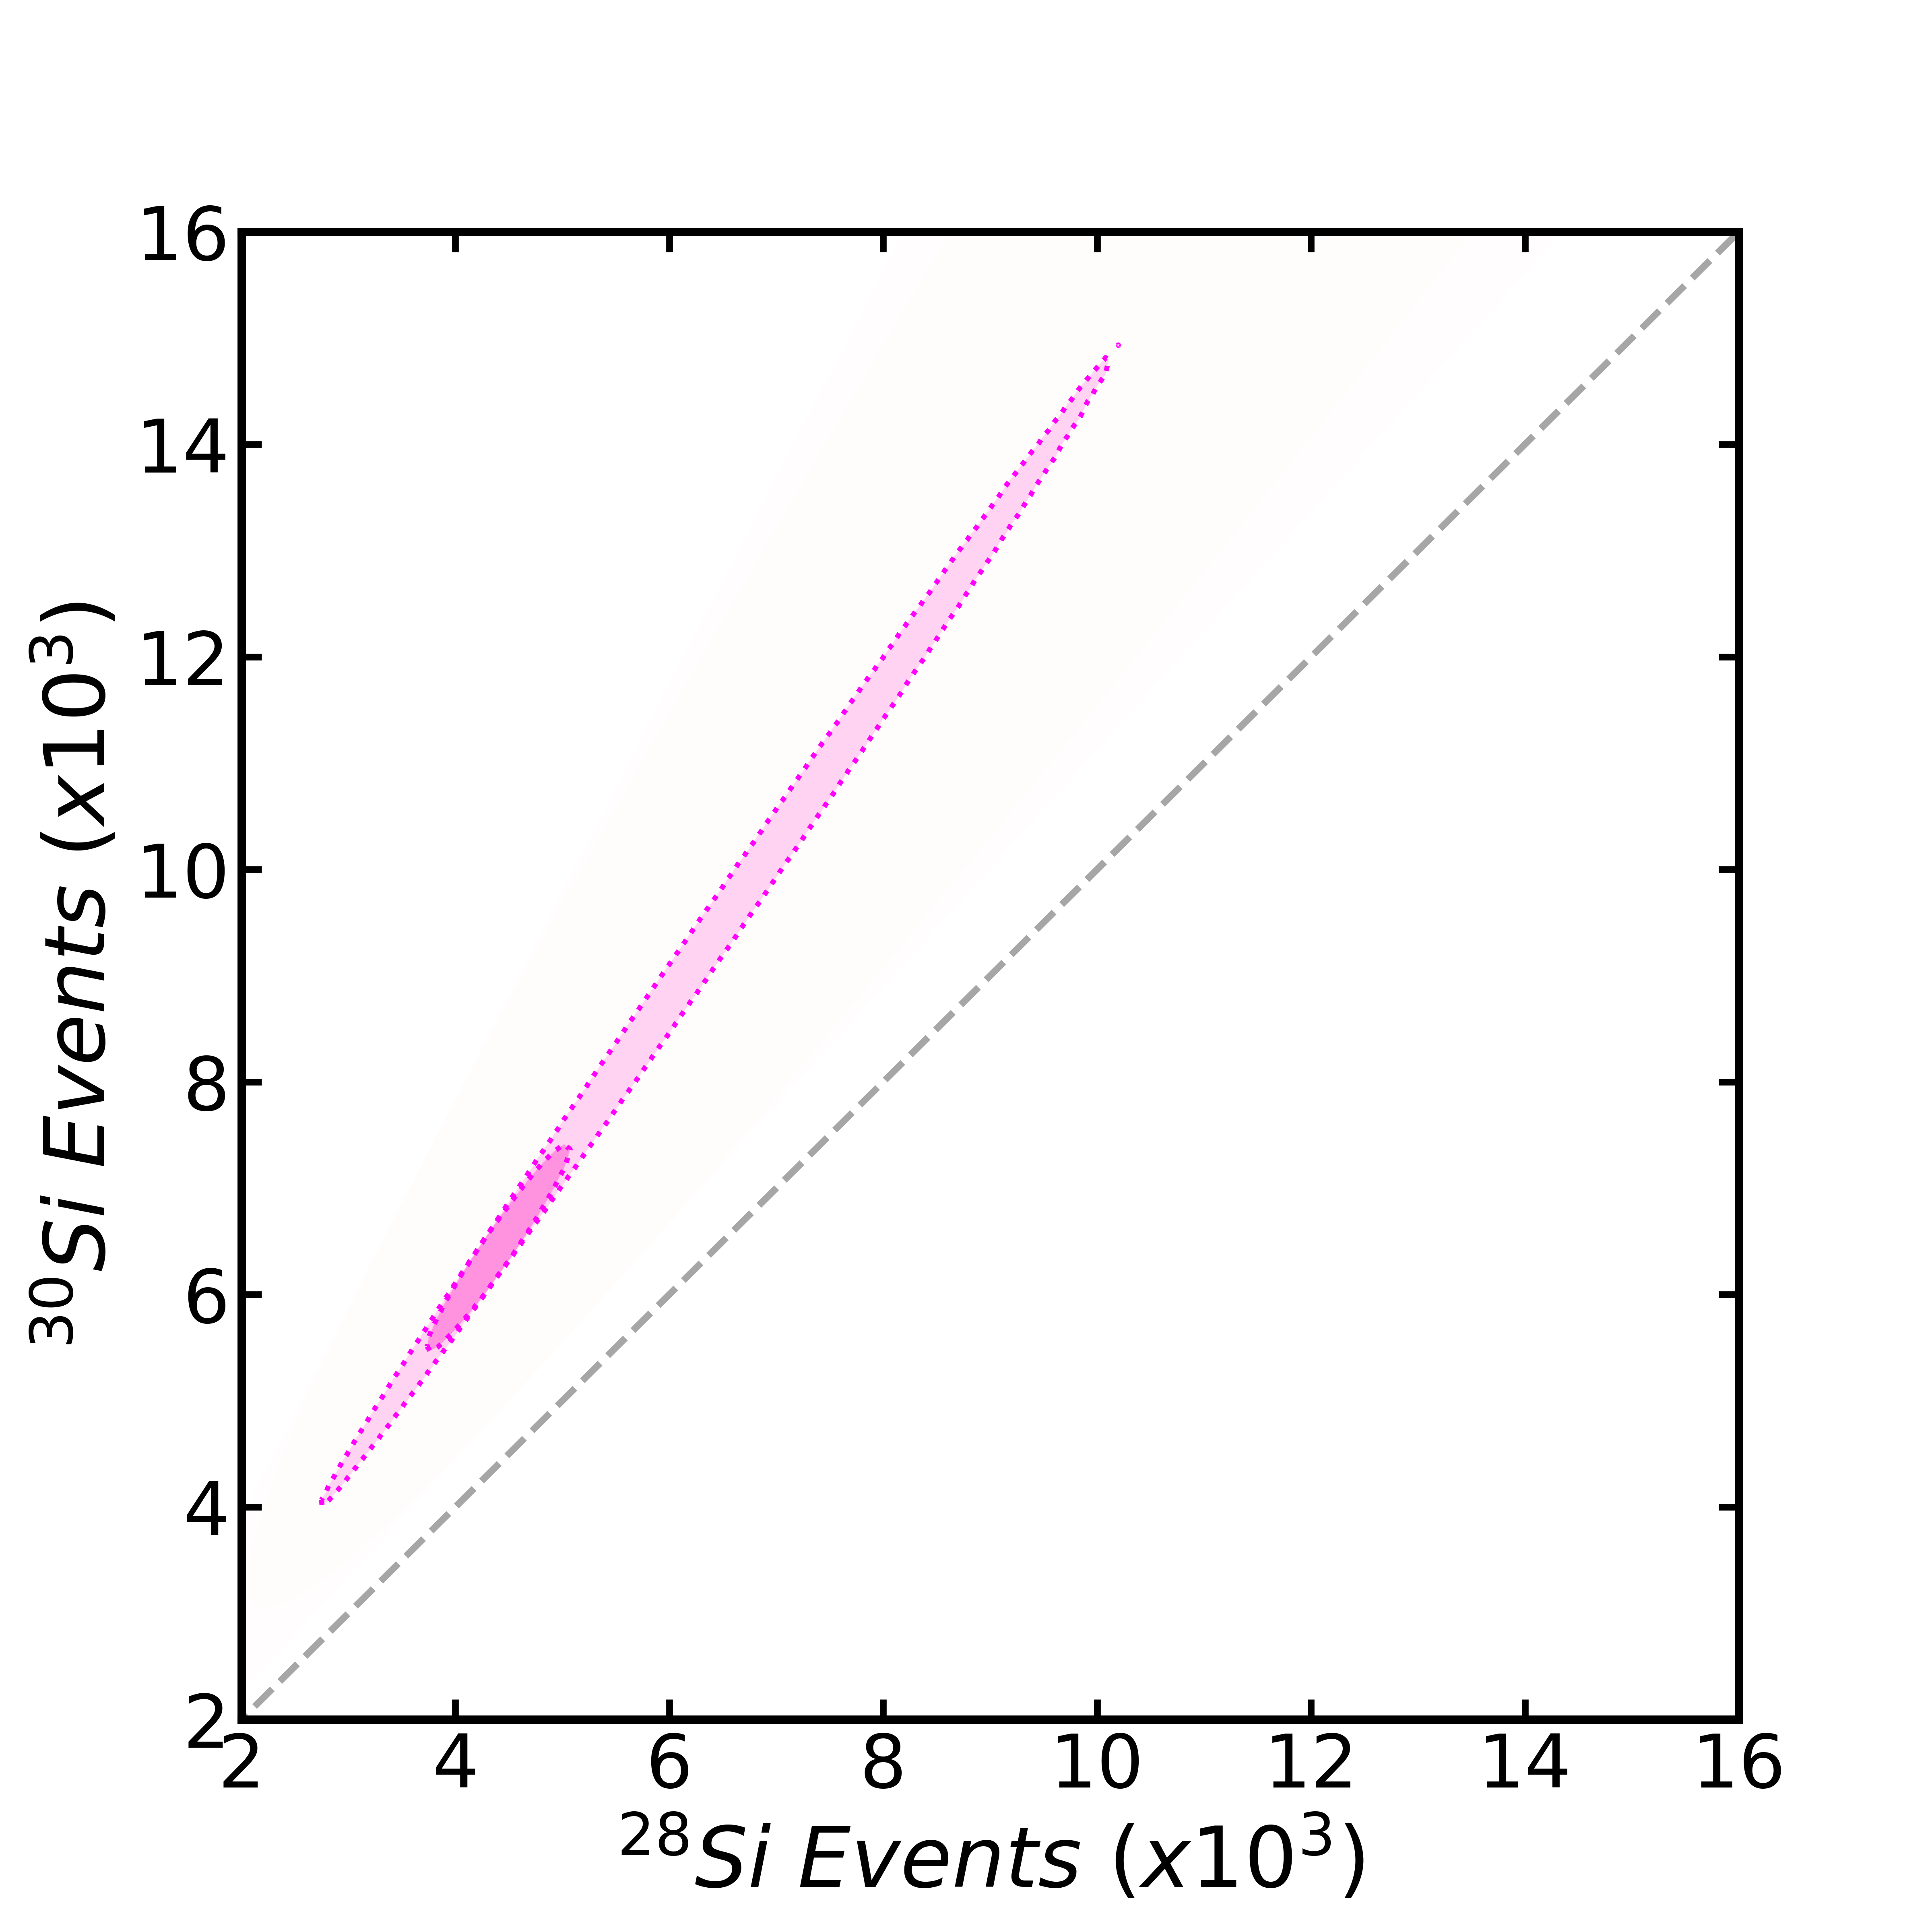
\includegraphics[scale=0.33]{figures/N2SiEvents7-1.png}}\hspace{-1em}
\subfigure[\emph{0.4 - 0.7 KeV}]{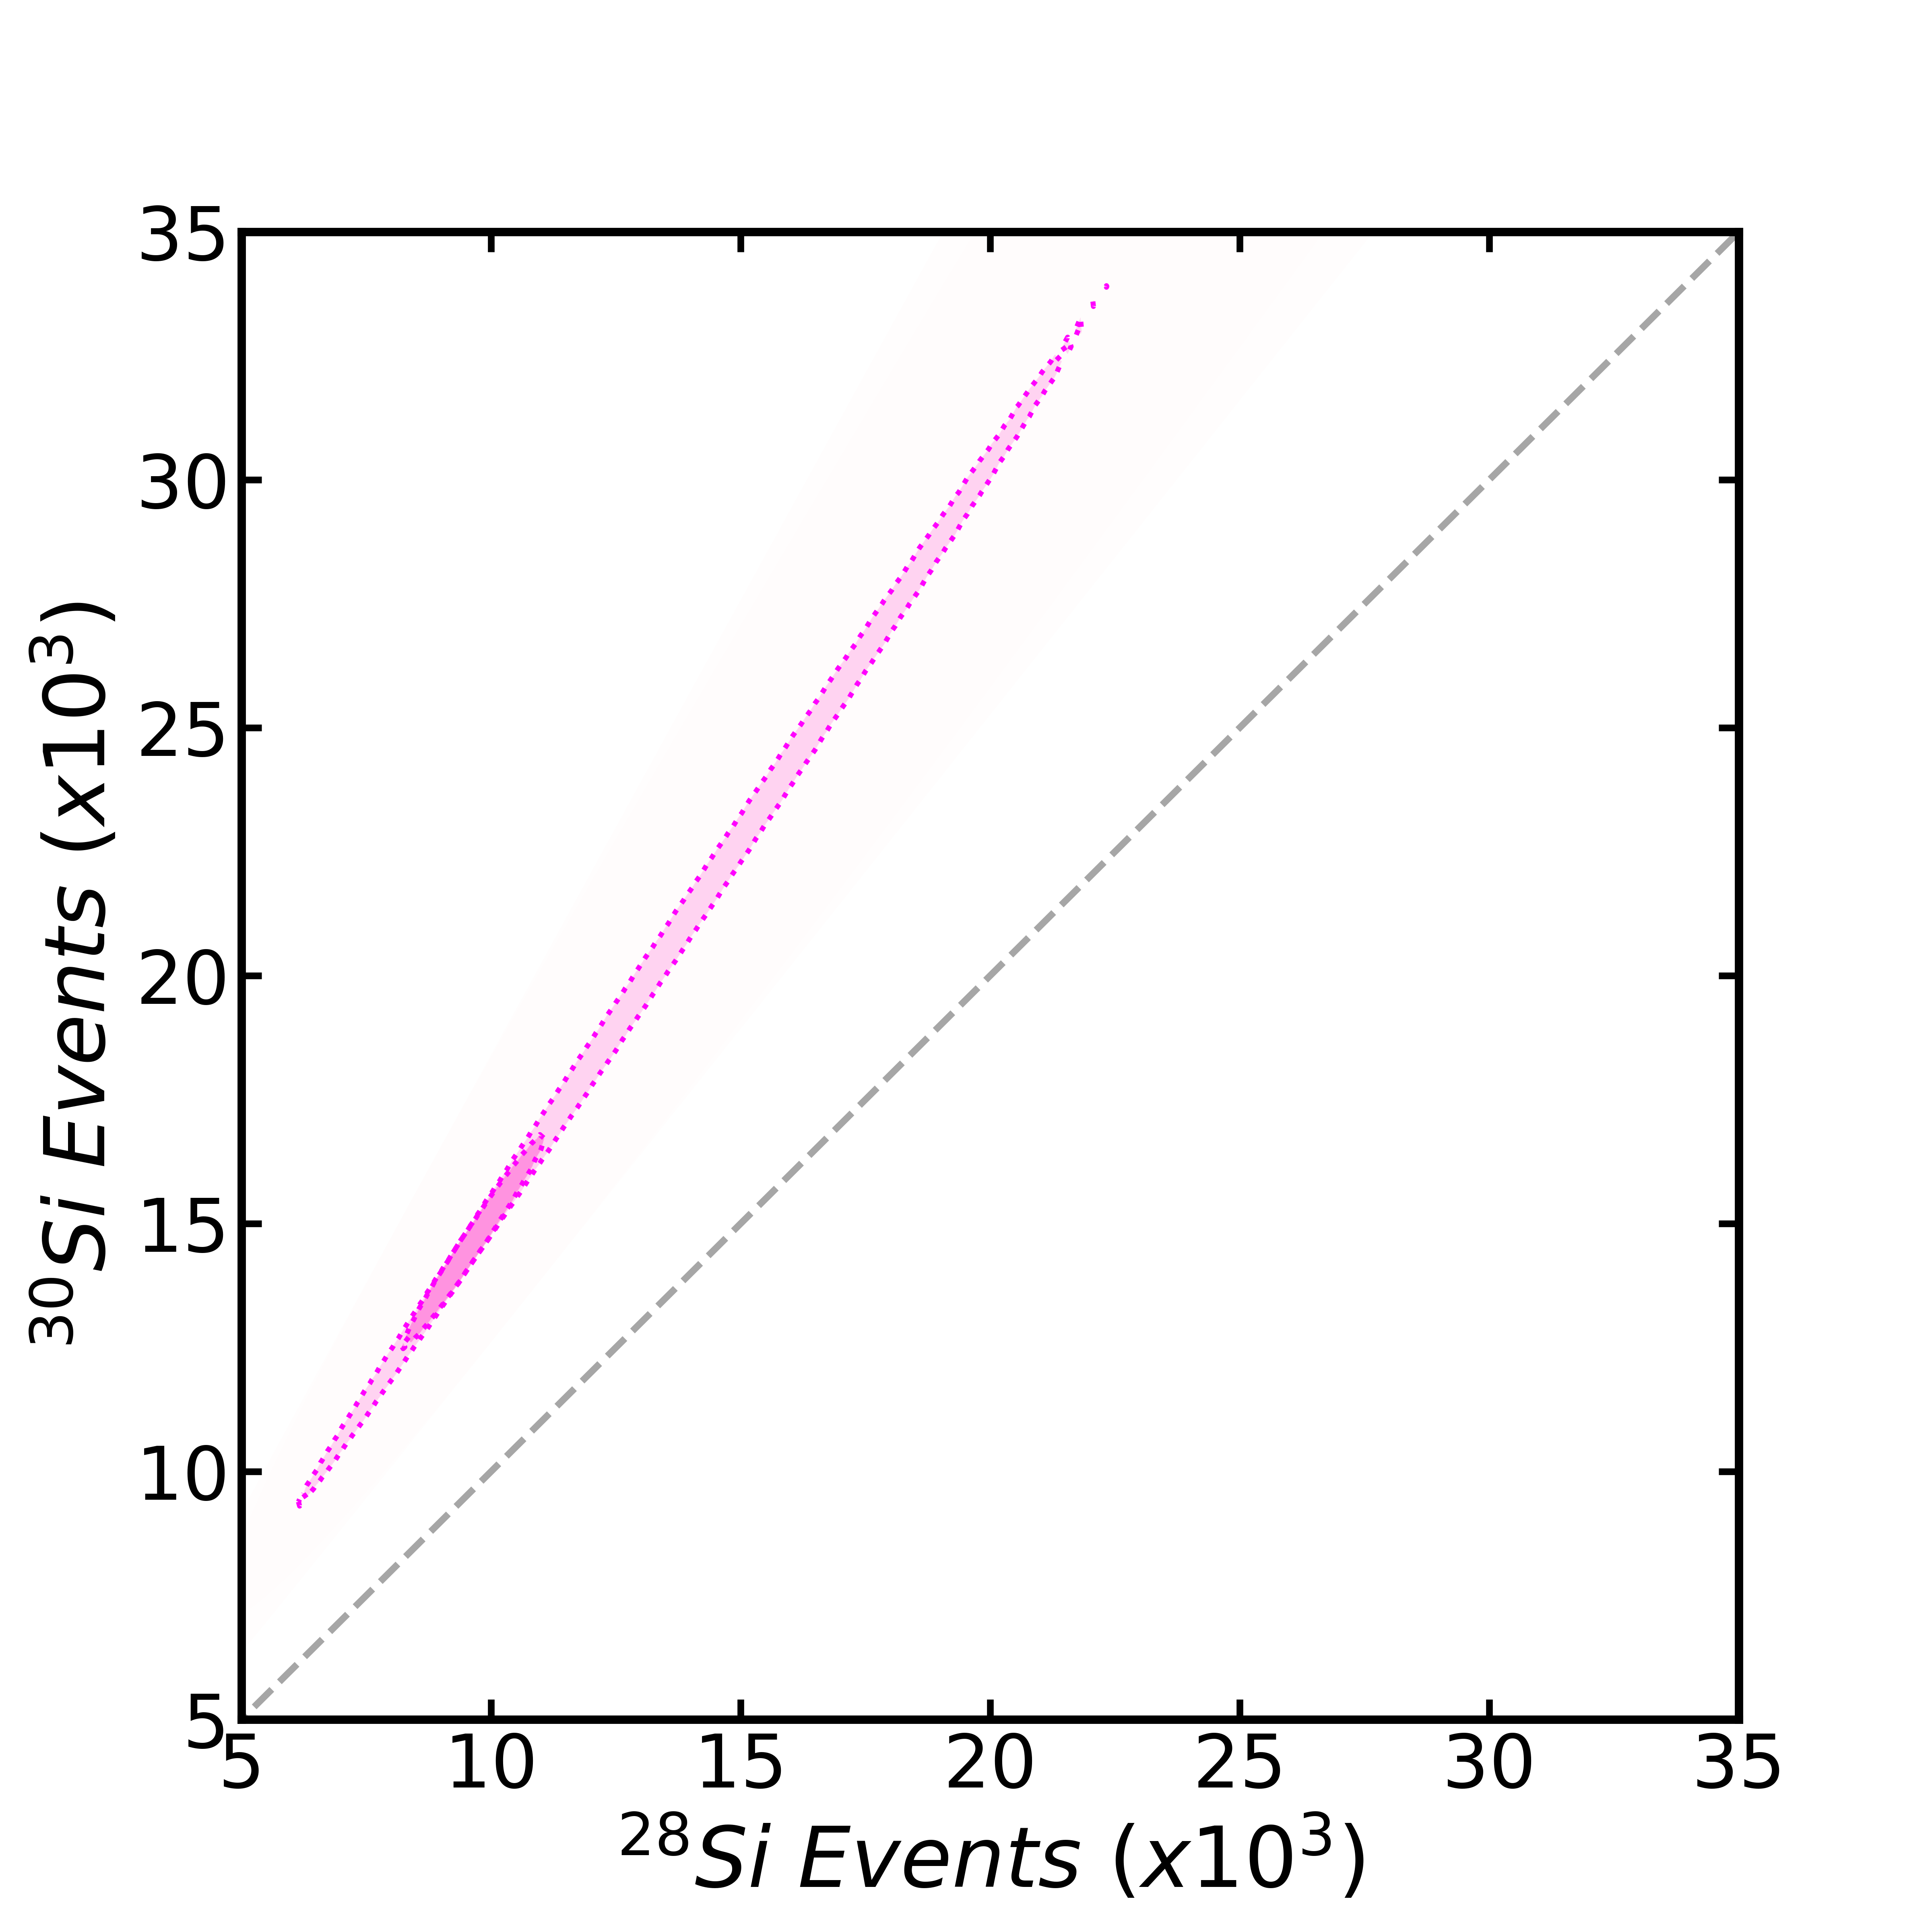
\includegraphics[scale=0.33]{figures/N2SiEvents4-7.png}}
\caption{Expected number of events for Si isotopes detector exposed to reactor antineutrino flux with different ranges of recoil energy. Light regions refer to the case of $\sigma_A = 25\%$ and $\sigma_B=10\%$ while dark regions refer to the case of $\sigma_A=\sigma_B=5\%$.In (a), the uncorrelated case is also shown in dashed lines.}
\label{N2EventsSi}
\end{figure}

In panel (a) of figure \ref{N2EventsSi}, the 2-3 KeV interval is depicted. This range is slightly above the crossover point, and here, it can be observed that the event numbers for both isotopes are very close to each other. In the 1-2 KeV region, we are already below the crossover point, and a slight increase in the event count from the heavier isotope is starting to become noticeable. This is shown in panel (b). Panels (c) and (d) depict the energy intervals of 0.7-1 KeV and 0.4-0.7 KeV. In both intervals, it is very clear that the heavier isotope has a higher number of events, confirming the quadratic dependence of the number of neutrons in the cross-section of this interaction.

Our analysis shows the following implications: The quadratic dependence of the number of neutrons $(N^2)$ is confirmed at very low recoil energies. However, it is important to consider that constructing detectors capable of experimentally reaching such extremely low energy thresholds is very challenging. Silicon emerges as a more suitable alternative to address this limitation. Its wider energy range provides a practical opportunity to experimentally validate the dependence within a more substantial and achievable energy interval.

In conclusion, while the Zinc isotopes analysis establishes the quadratic dependence at lower energies, the Silicon isotopes analysis extends this confirmation to higher and more achievable energy ranges, making Silicon a more suitable material for experimental validation.


\section{Constraining non-standard interactions parameters}

Neutrino non-standard interactions (NSIs) represent hypothetical phenomena beyond the Standard Model. According to the Standard Model, neutrinos interact with matter exclusively through the weak nuclear force and experience the negligible influence of gravity. NSIs, if proven to exist, would introduce the possibility that neutrinos can also interact with matter through alternative forces or mechanisms not considered by the Standard Model. These interactions can affect the propagation and oscillation of neutrinos through matter, impacting their flavor-changing properties and scattering processes.

Considering that CE$\nu$NS is a neutral current process, it will be affected by non-standard neutral current interactions, typically described as follows \cite{Dev_2019}:
\begin{equation}
    \mathcal{L}^{NC}=-2\sqrt{2}G_F \sum_{f,P,\alpha,\beta} \varepsilon_{\alpha \beta}^{f,P} \left(\bar\nu_\alpha\gamma^\mu P_L \nu_\beta\right)\left(\bar f \gamma_\mu P f\right),
\end{equation}
where $G_F$ is Fermi's constant and the $\varepsilon_{\alpha \beta}^{f, P}$ parameters are related to the magnitude of the NSI's in relation to the weak force scale. Here $\alpha$ and $\beta$ indicate the neutrino flavors ($e$, $\mu$, $\tau$) and $f$ is a matter fermion ($e$, $u$, $d$). $P$ denotes the chirality projector operator, which can be expressed as $P_L, P_R = \left(1\pm \gamma^5\right)/2$, and can also be transformed into the vector and axial components of the interaction.\\
Taking this into account and noting that the interaction in CE$\nu$NS is the scattering of a neutrino with a nucleus, we obtain
\begin{equation}
    \mathcal{L}_{\nu N}^{NC} =- \frac{G_F}{\sqrt{2}} \sum_{q,\alpha,\beta} \left[\bar\nu_\alpha \gamma^\mu\left(1-\gamma^5\right)\nu_\beta\right] \left(\varepsilon^{qL}_{\alpha \beta} \left[\bar q \gamma_\mu \left(1-\gamma^5\right)q \right] + \varepsilon^{qR}_{\alpha \beta} \left[\bar q \gamma_\mu \left(1+\gamma^5\right)q\right]\right).
\end{equation}
Here, q runs over the quarks within the nucleons, that is, over $u$ and $d$. As mentioned previously, it is possible to transform the parameters to obtain the vector and axial components of the interaction
\begin{align*}
    \varepsilon_{\alpha \beta}^{qV}=\varepsilon_{\alpha \beta }^{qL}+\varepsilon_{\alpha \beta}^{qR},     \\[1.5em]    
 \varepsilon_{\alpha \beta}^{qA}=\varepsilon_{\alpha \beta }^{qL}-\varepsilon_{\alpha \beta}^{qR}.
\end{align*}
But we are exclusively taking into account the vector components of the non-standard interaction, given that, in the context of CE$\nu$NS, the axial components are significantly suppressed \cite{Barranco_2005}. The $\varepsilon_{\alpha \alpha}^{qV}$  parameters are referred to as "non-universal" because they serve as a mechanism for breaking lepton flavor universality, while the $\varepsilon_{\alpha \beta}^{qV} \left(\alpha \neq \beta\right)$ parameters are known as flavor-changing.


Therefore, the weak nuclear charge takes on the following form when non-standard interactions are incorporated:
\begin{equation*}
\begin{split}
\mathcal{Q}_W^2
    &=\phantom{-}\left[Z\left(g_V^p +2\varepsilon_{\alpha \alpha}^{uV}+\varepsilon_{\alpha \alpha}^{dV}\right)+N \left(g_V^n + \varepsilon _{\alpha \alpha}^{uV}+2\varepsilon_{\alpha \alpha}^{dV}\right)\right]^2\\
    &\quad\smash[b]+ \sum_{\beta\neq\alpha} \left[Z\left(2\varepsilon_{\beta \alpha}^{uV}+\varepsilon_{\beta \alpha}^{dV}\right) + N \left(\varepsilon_{ \beta \alpha}^{uV}+2\varepsilon_{\beta \alpha}^{dV}\right)\right]^2.
\end{split}
\end{equation*}

Once again, this modifies the effective cross-section of CE$\nu$NS previously presented in Chapter 2, as shown below \cite{Barranco_2005}
\begin{equation}
\begin{split}
\frac{d \sigma}{dT} 
&\simeq \phantom{-}\frac{G^2_F M}{\pi} \left(1-\frac{MT}{2E^2_\nu}\right) F^2(q^2)\biggl\{ \left[Z \left(g^p_V +2 \varepsilon_{\alpha \alpha}^{uV} + \varepsilon_{\alpha \alpha}^{dV}\right) + N \left(g_V^{n} + \varepsilon_{\alpha \alpha}^{uV} + 2 \varepsilon_{\alpha \alpha}^{dV}\right) \right]^2\\ 
&\quad\smash[b]+ \sum_{\beta \neq \alpha} \left[Z \left(2 \varepsilon_{\beta \alpha}^{uV}+\varepsilon
_{\beta \alpha}^{dV}\right) + N\left(\varepsilon_{\beta \alpha}^{uV} + 2\varepsilon_{\beta \alpha}^{dV}\right)\right]^2 \biggr\}.
\end{split}
\end{equation}
Using this expression for the cross-section, we will calculate the number of events, enabling us to conduct an analysis similar to what has been previously done in this section. This analysis aims to study the sensitivity to the proposed detectors' non-standard interactions (NSIs), considering both  $\pi$-DAR and reactor flux.



\begin{figure}[h!]
\centering
\subfigure{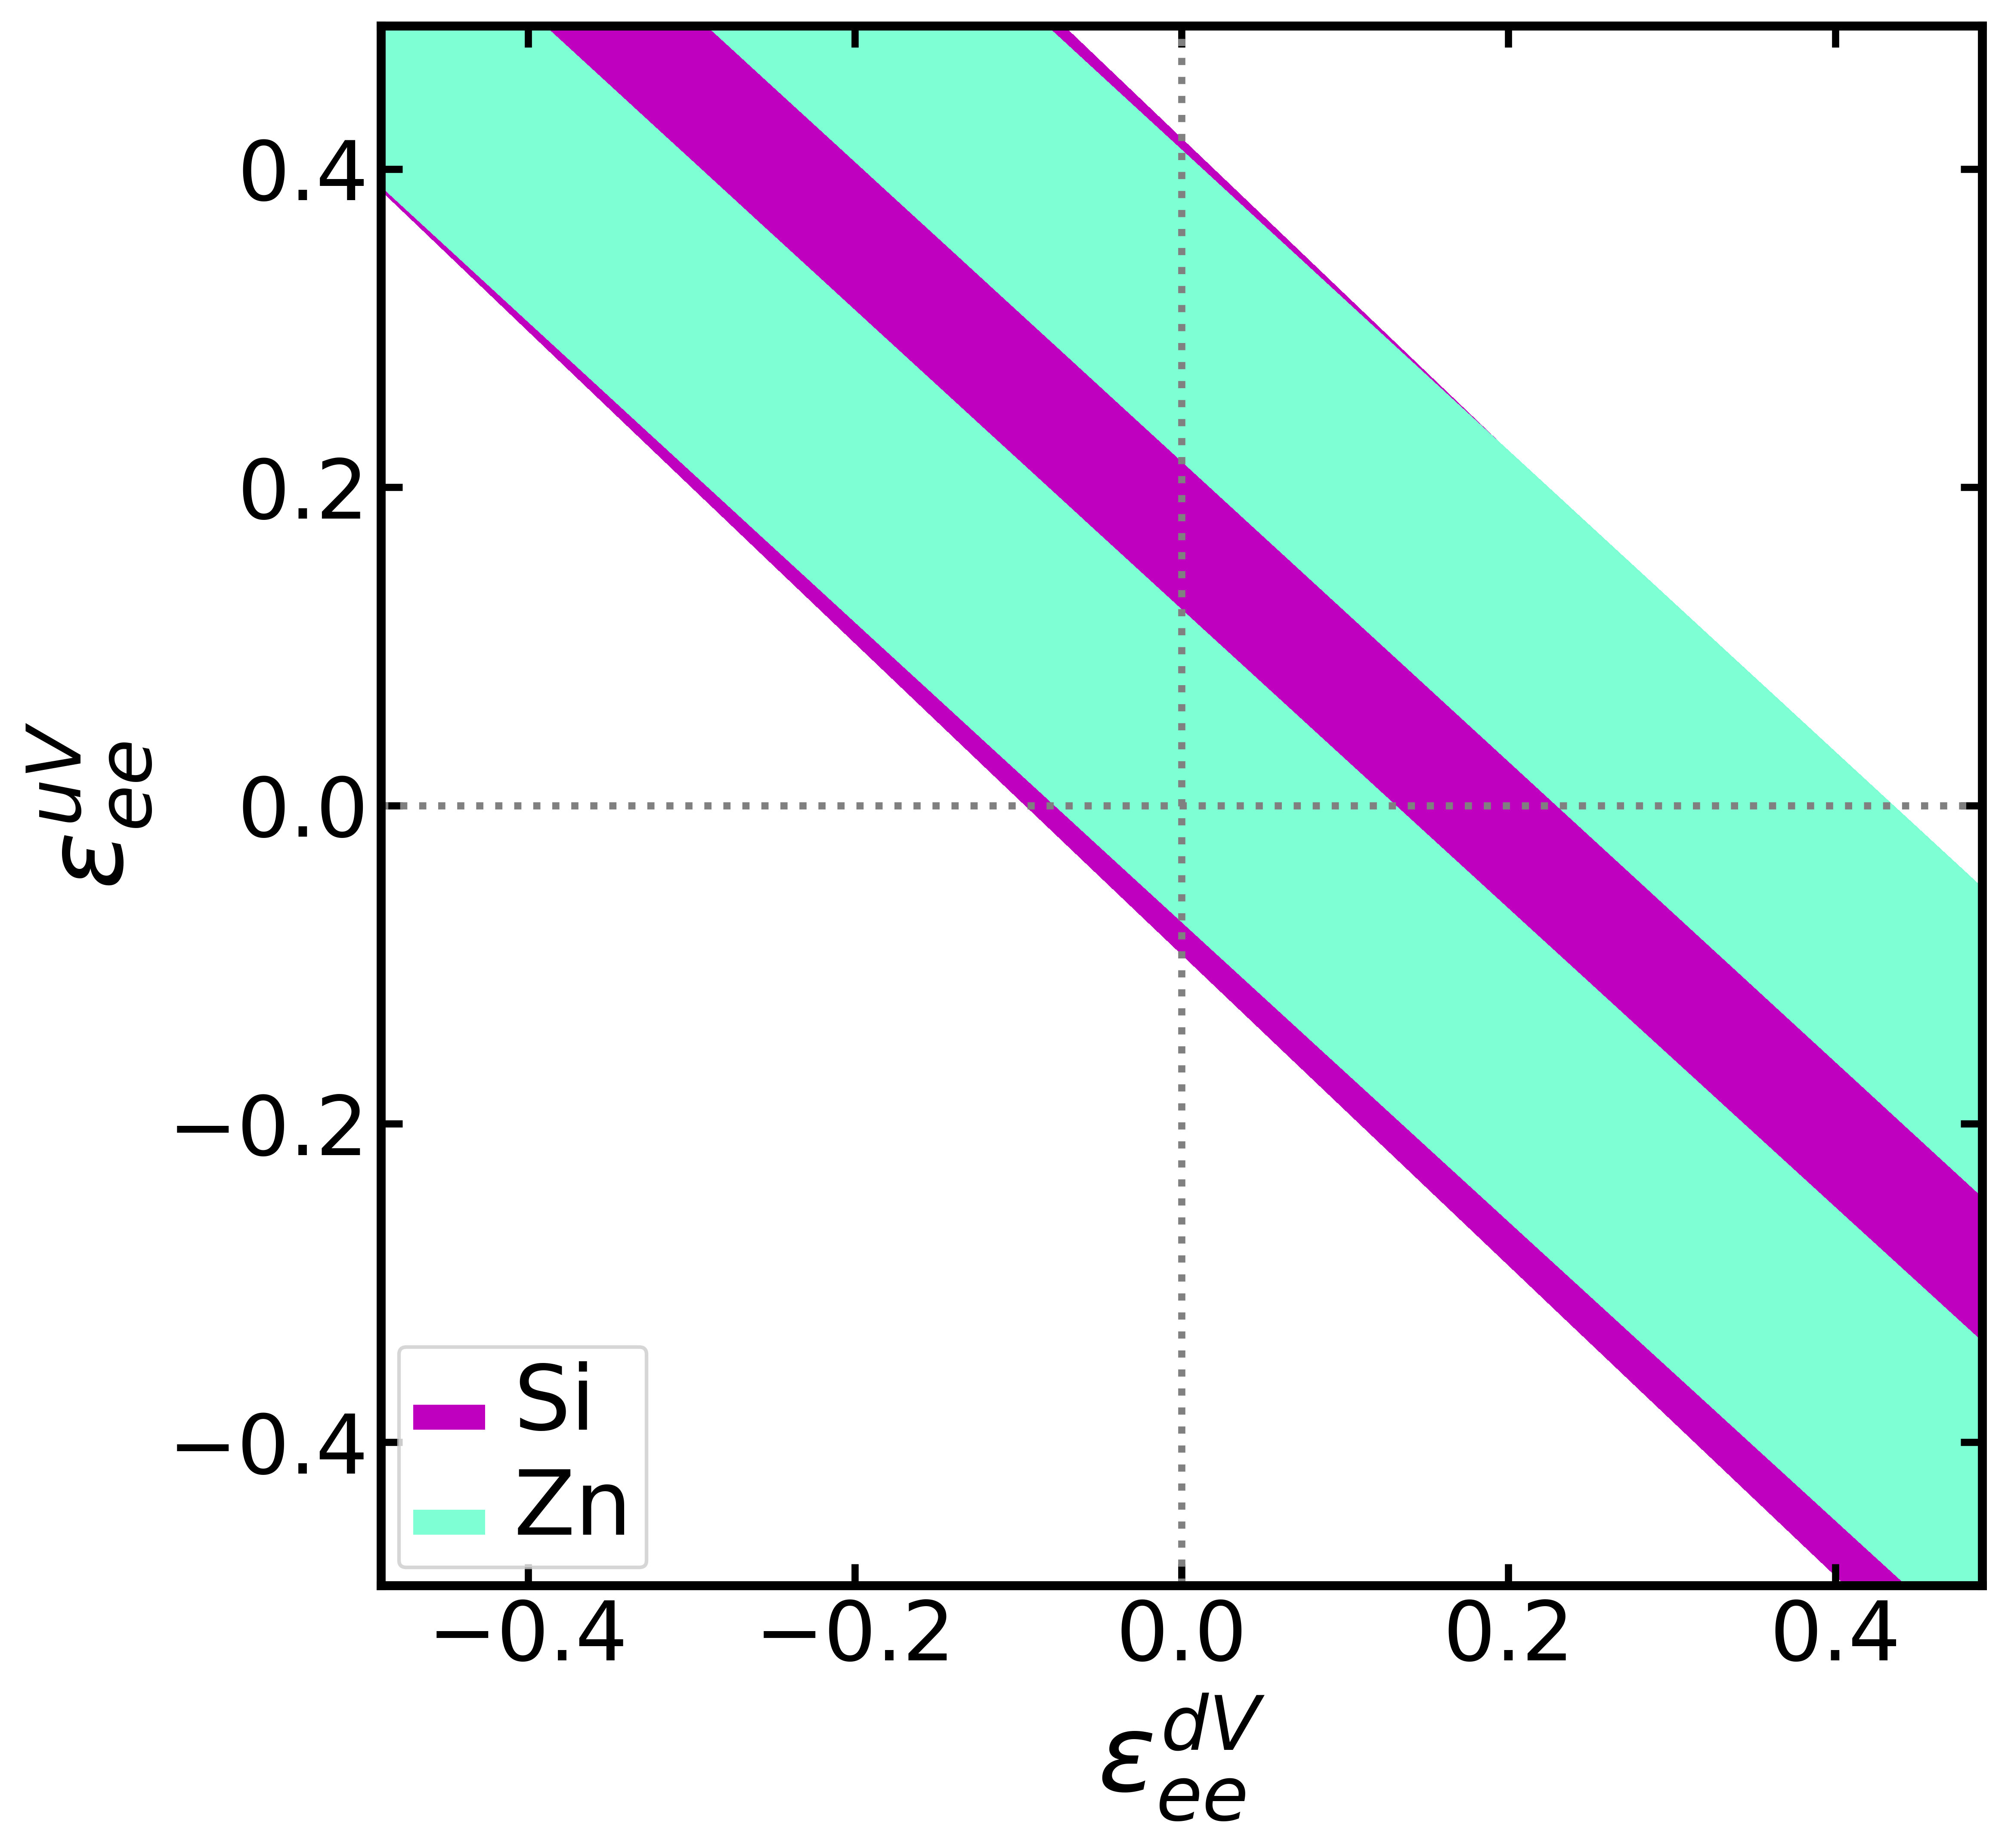
\includegraphics[scale=0.33]{figures/NSIEESNS.png}}\hspace{1em}%
\subfigure{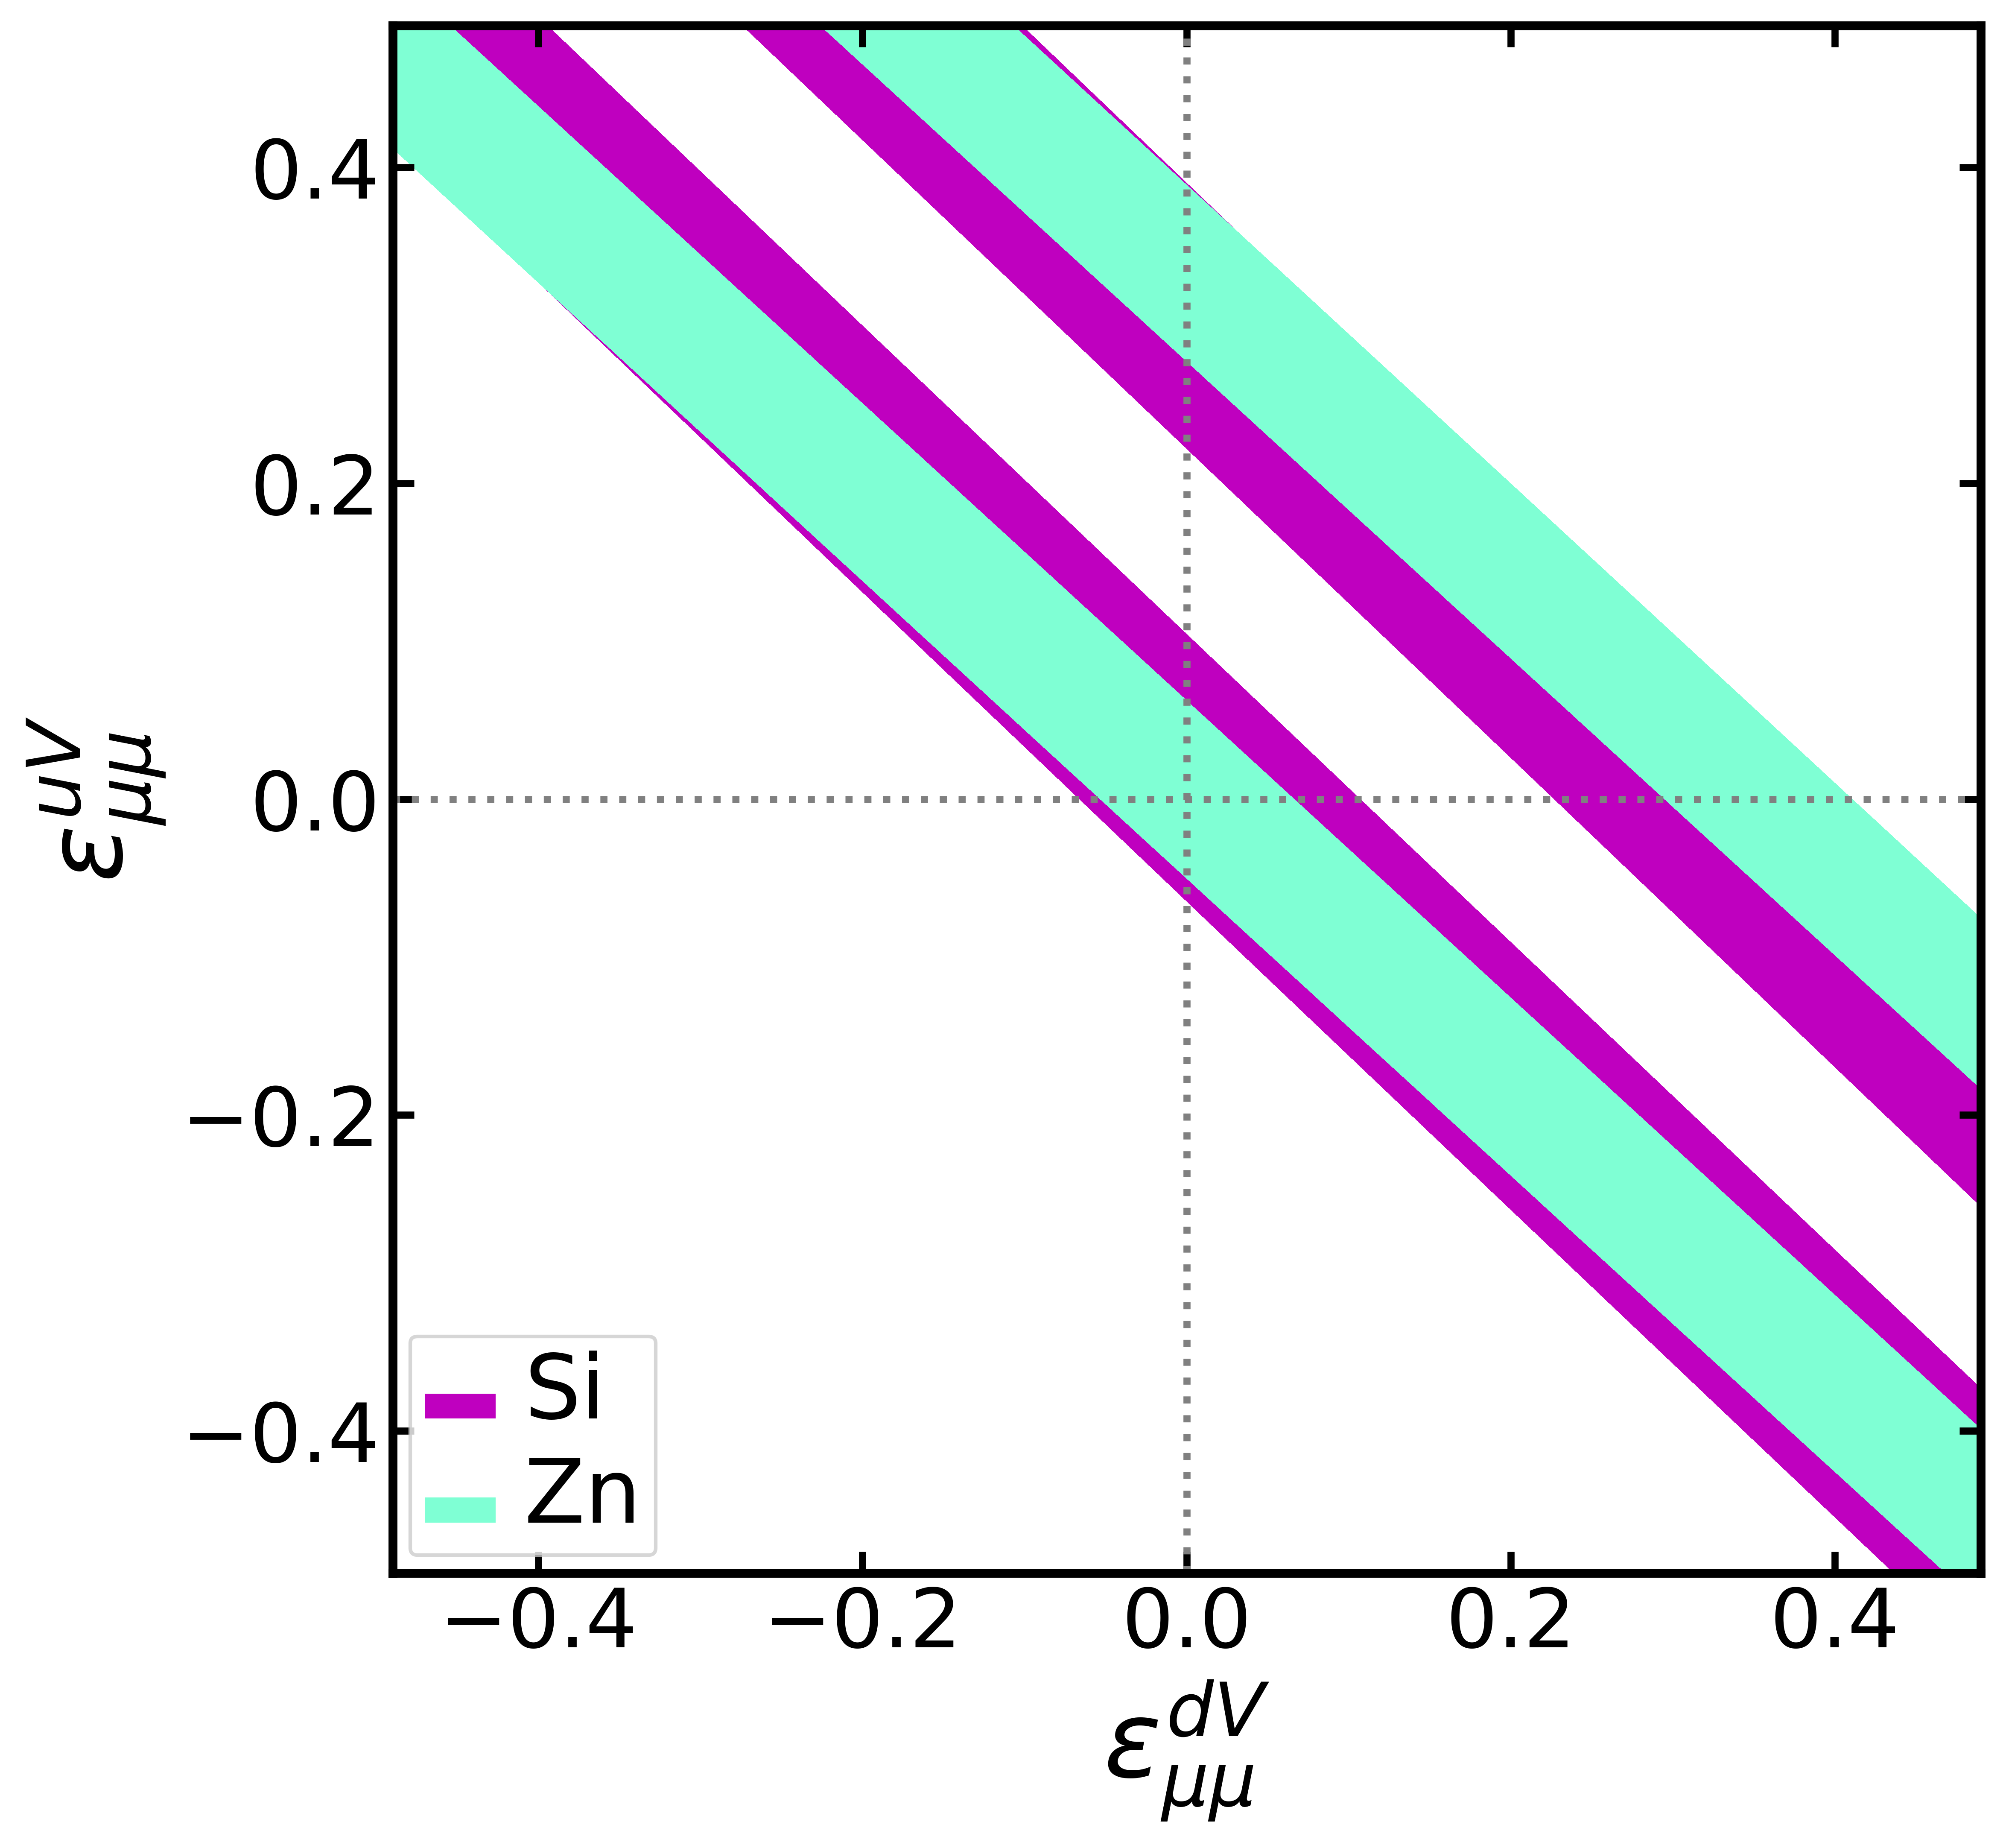
\includegraphics[scale=0.33]{figures/NSImuSNS.png}}\par\vspace{0em}%
\subfigure{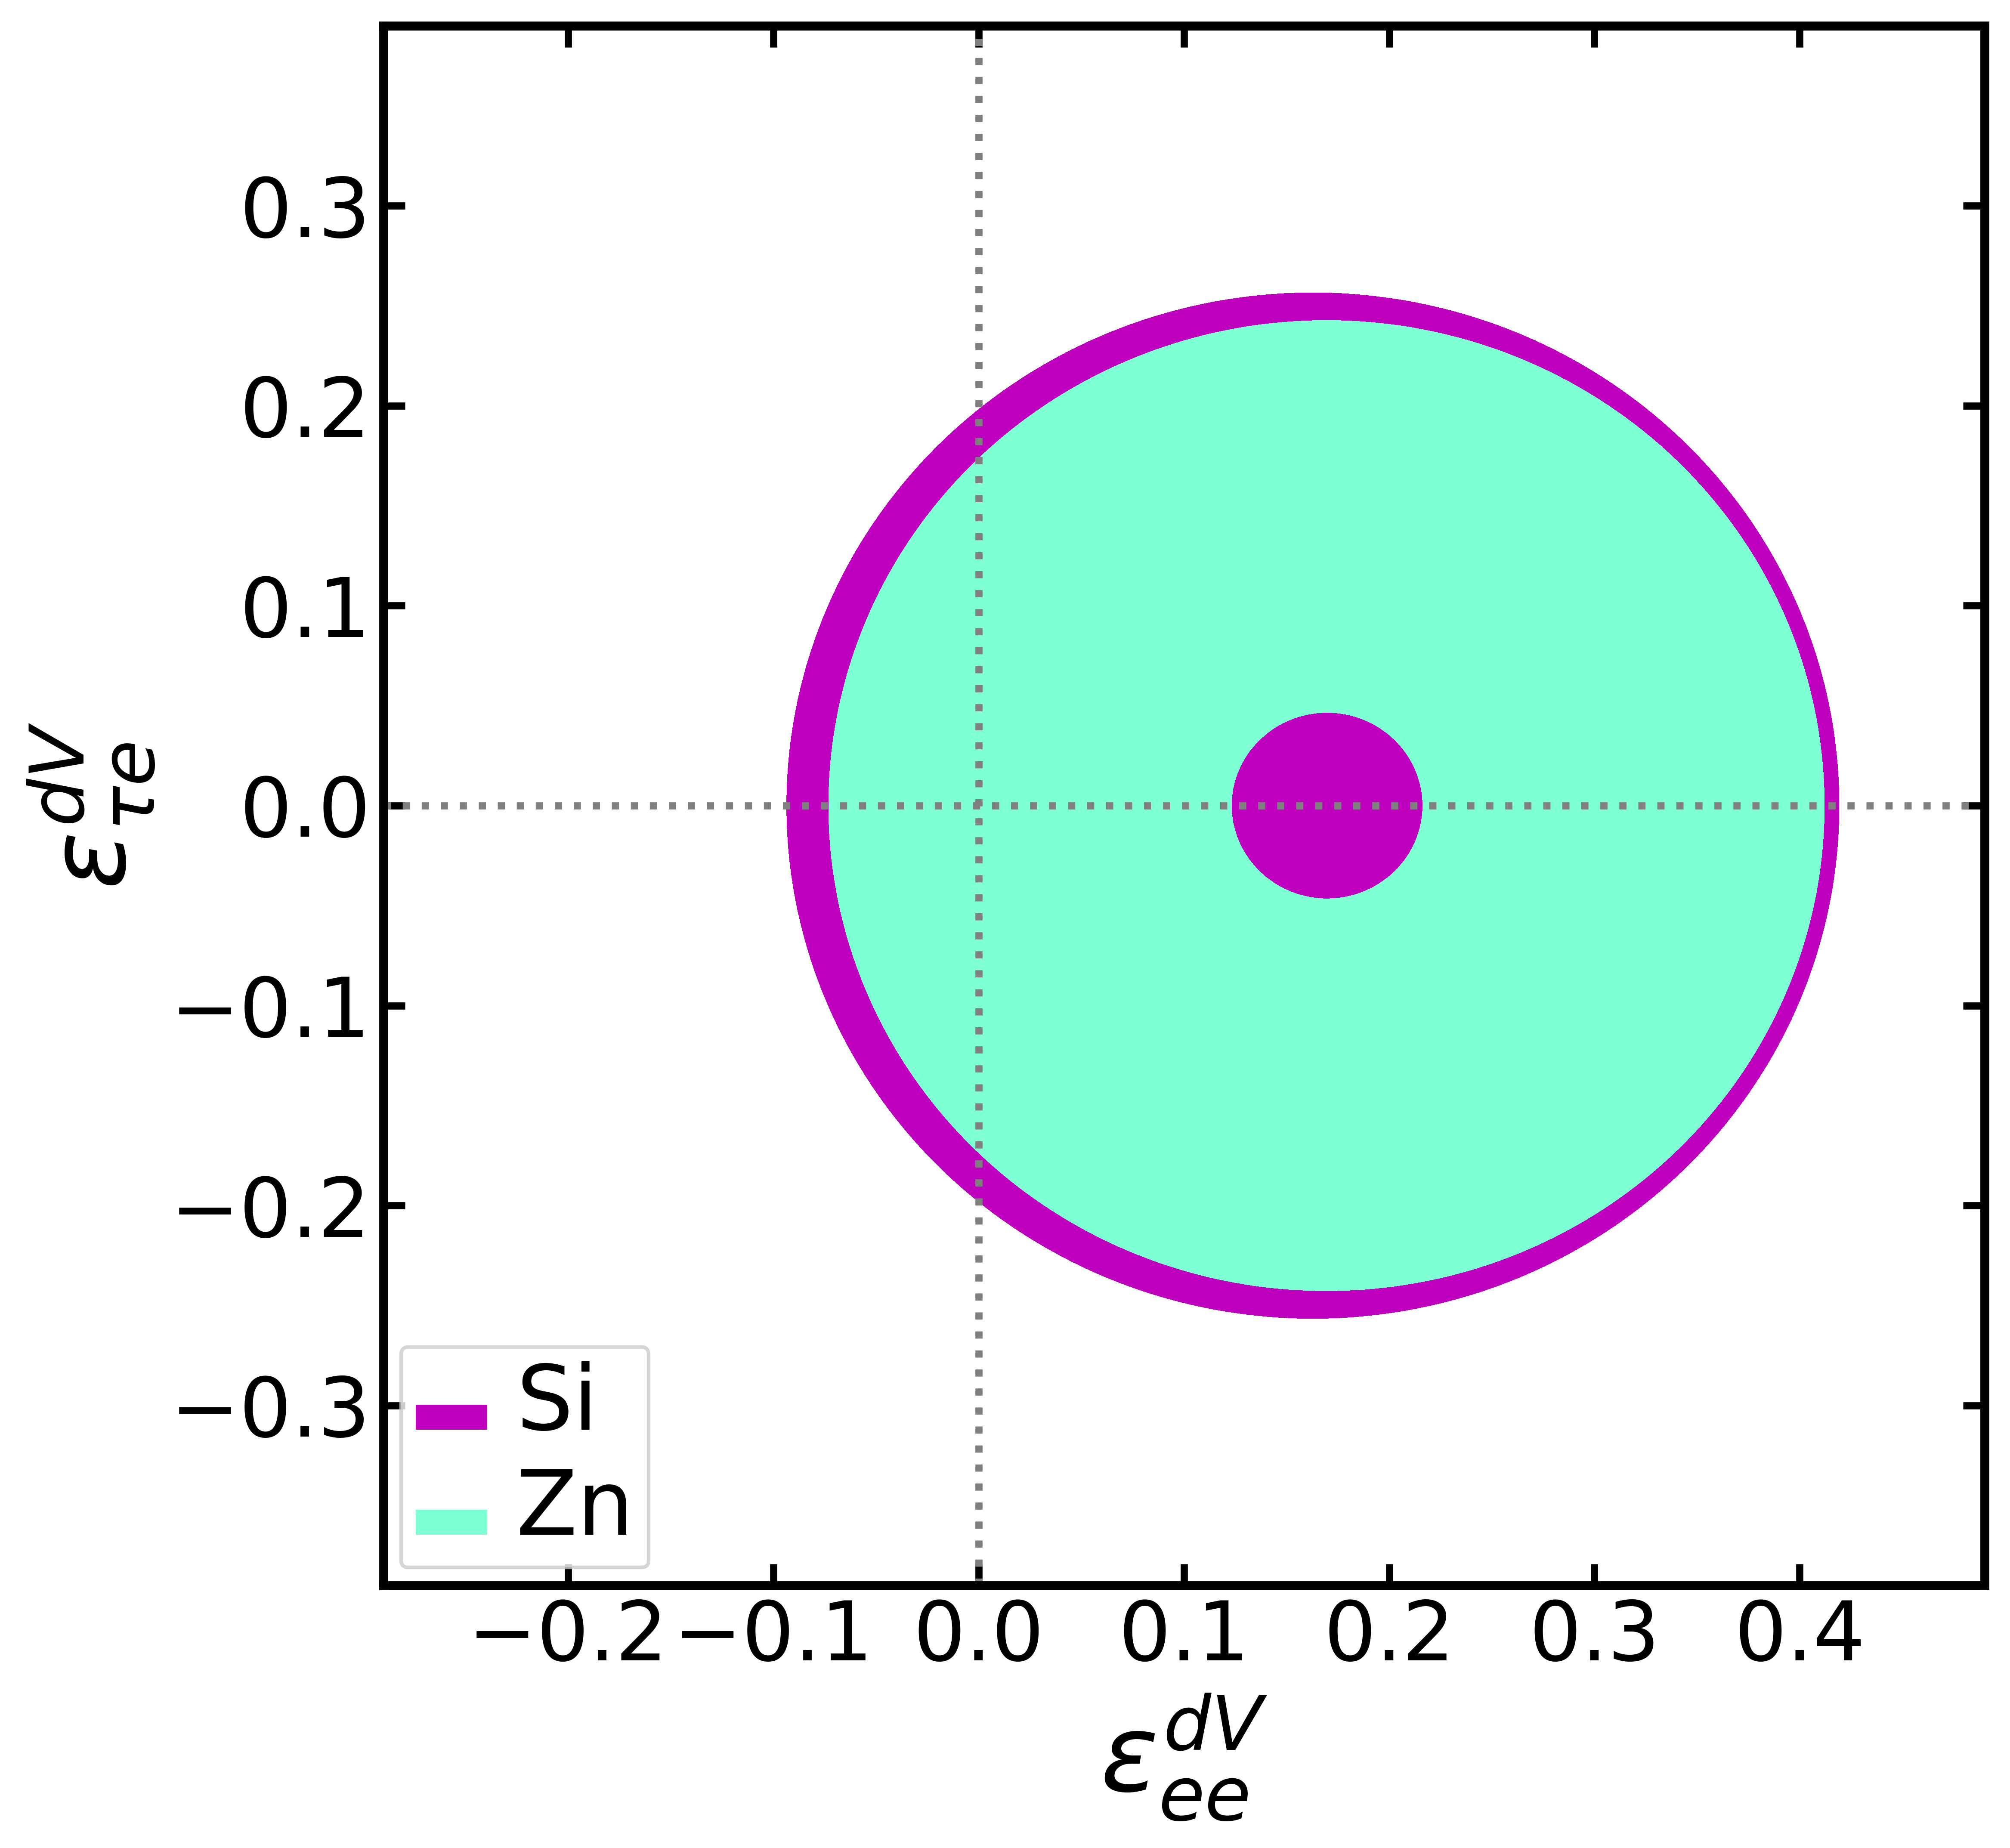
\includegraphics[scale=0.33]{figures/NSIEmuSNS.png}}
\caption{Expected allowed values for the NSIs parameters at a 90$\%$ confidence level for the detectors exposed to a $\pi$-DAR flux. The purple regions correspond to the Si detectors, while the cyan regions correspond to the Zn detectors. }
\label{SNS NSIs}
\end{figure}
Fig \ref{SNS NSIs}  displays the analysis results using the flux from $\pi$-DAR. Two parameters were simultaneously constrained. In the upper part of the graph, you can see the expected allowed regions for the non-universal parameters, both for the electron neutrino ($\nu_e$) component and the muon neutrino ($\nu_\mu$) components. Notably, the second case shows a slight improvement compared to the first because, in this flux, we have two components of muon neutrinos ($\nu_\mu$, and $\bar\nu_{\mu}$), resulting in higher statistics. 
The lower part of the graph illustrates the constraint on the flavor-changing parameter $\varepsilon_{\tau e}^{dV}$ and the non-universal parameter $\varepsilon_{ee}^{dV}$. The muon neutrino flavor-changing parameters have substantial restrictions from other experiments, so we consider the flavor-changing parameter related to tau neutrinos. This pair of parameters has been selected because it allows a direct comparison with the case where the reactor flux is considered.

We carry out this analysis using an antineutrino flux from a reactor. It is important to recall that this flux consists only of electron antineutrinos ($\bar\nu_e$), so we can exclusively analyze the parameters related to alpha ($\alpha=e$). 
As observed in the case of the $\pi$-DAR flux, constraining two NSI parameters simultaneously can lead to degeneracies in their values. Fig \ref{Reactor-NU} shows the analysis using the reactor flux, and it is noticeable that not only are the values much more restricted but the degeneracy in their values is broken within a specific range when the correlation between detectors is taken into account.





\begin{figure}[h!]
\centering
\subfigure{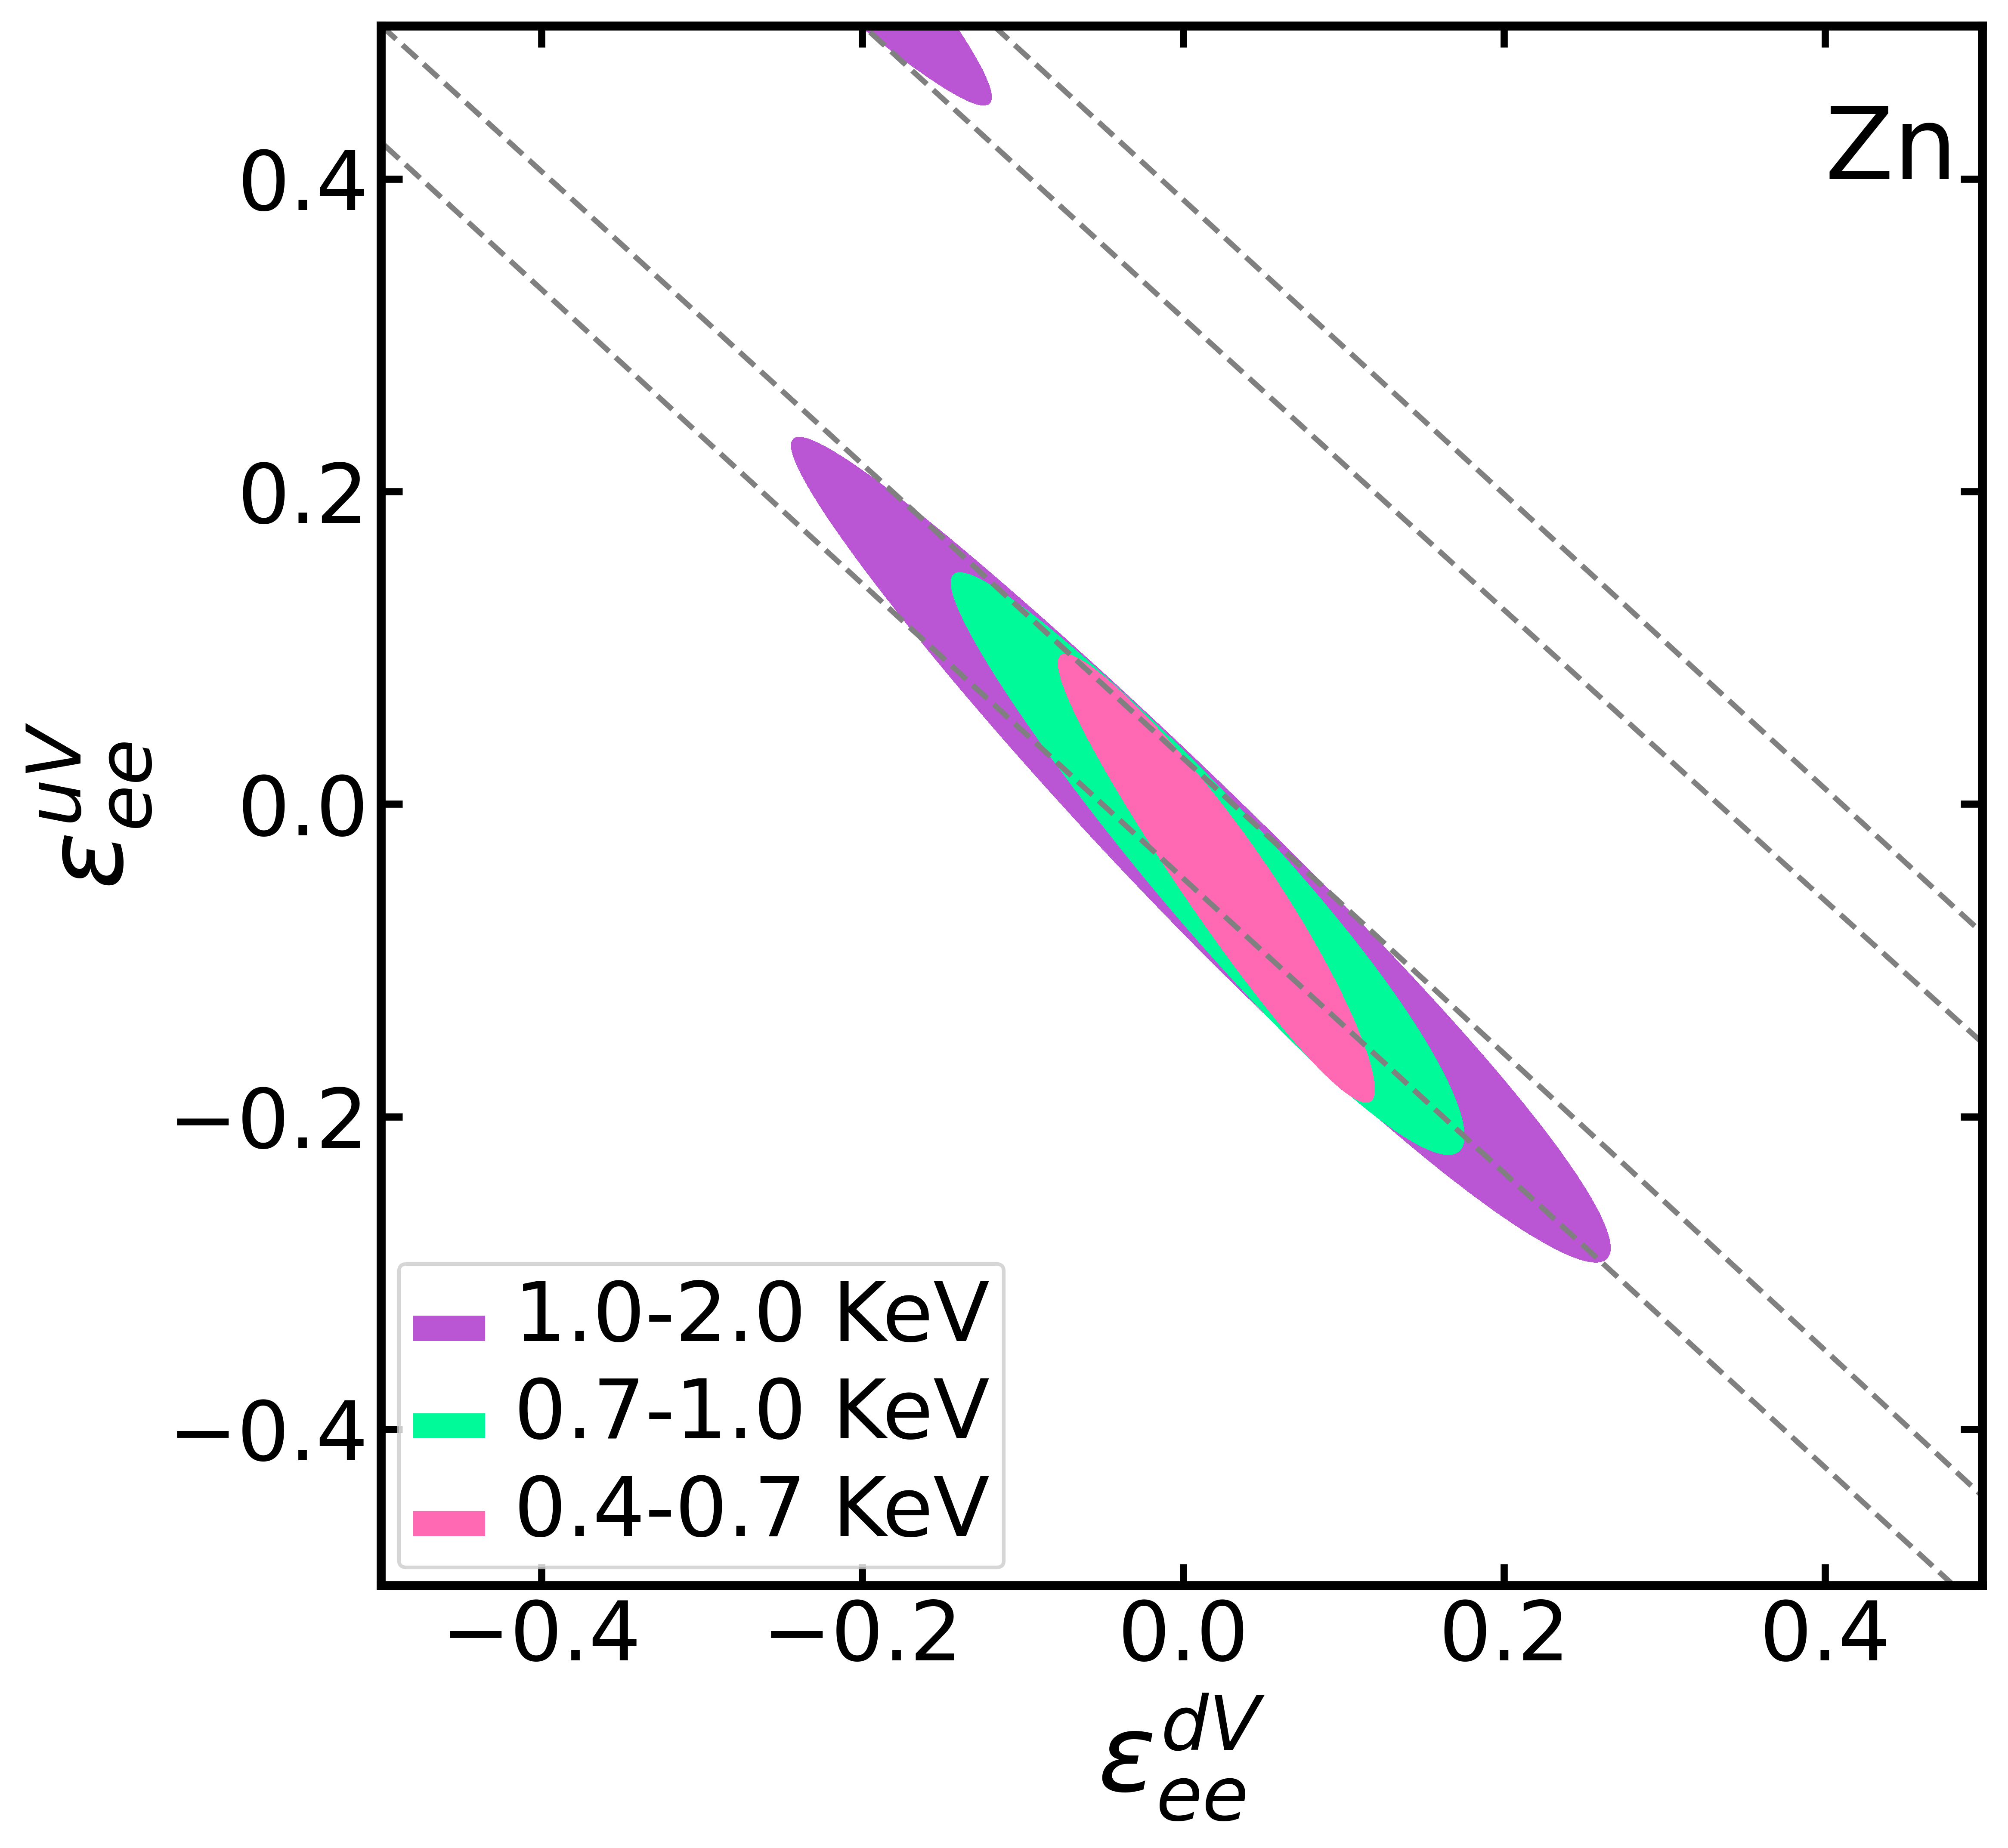
\includegraphics[scale=0.33]{figures/NSIZndVu.png}}\hspace{1em}%
\subfigure{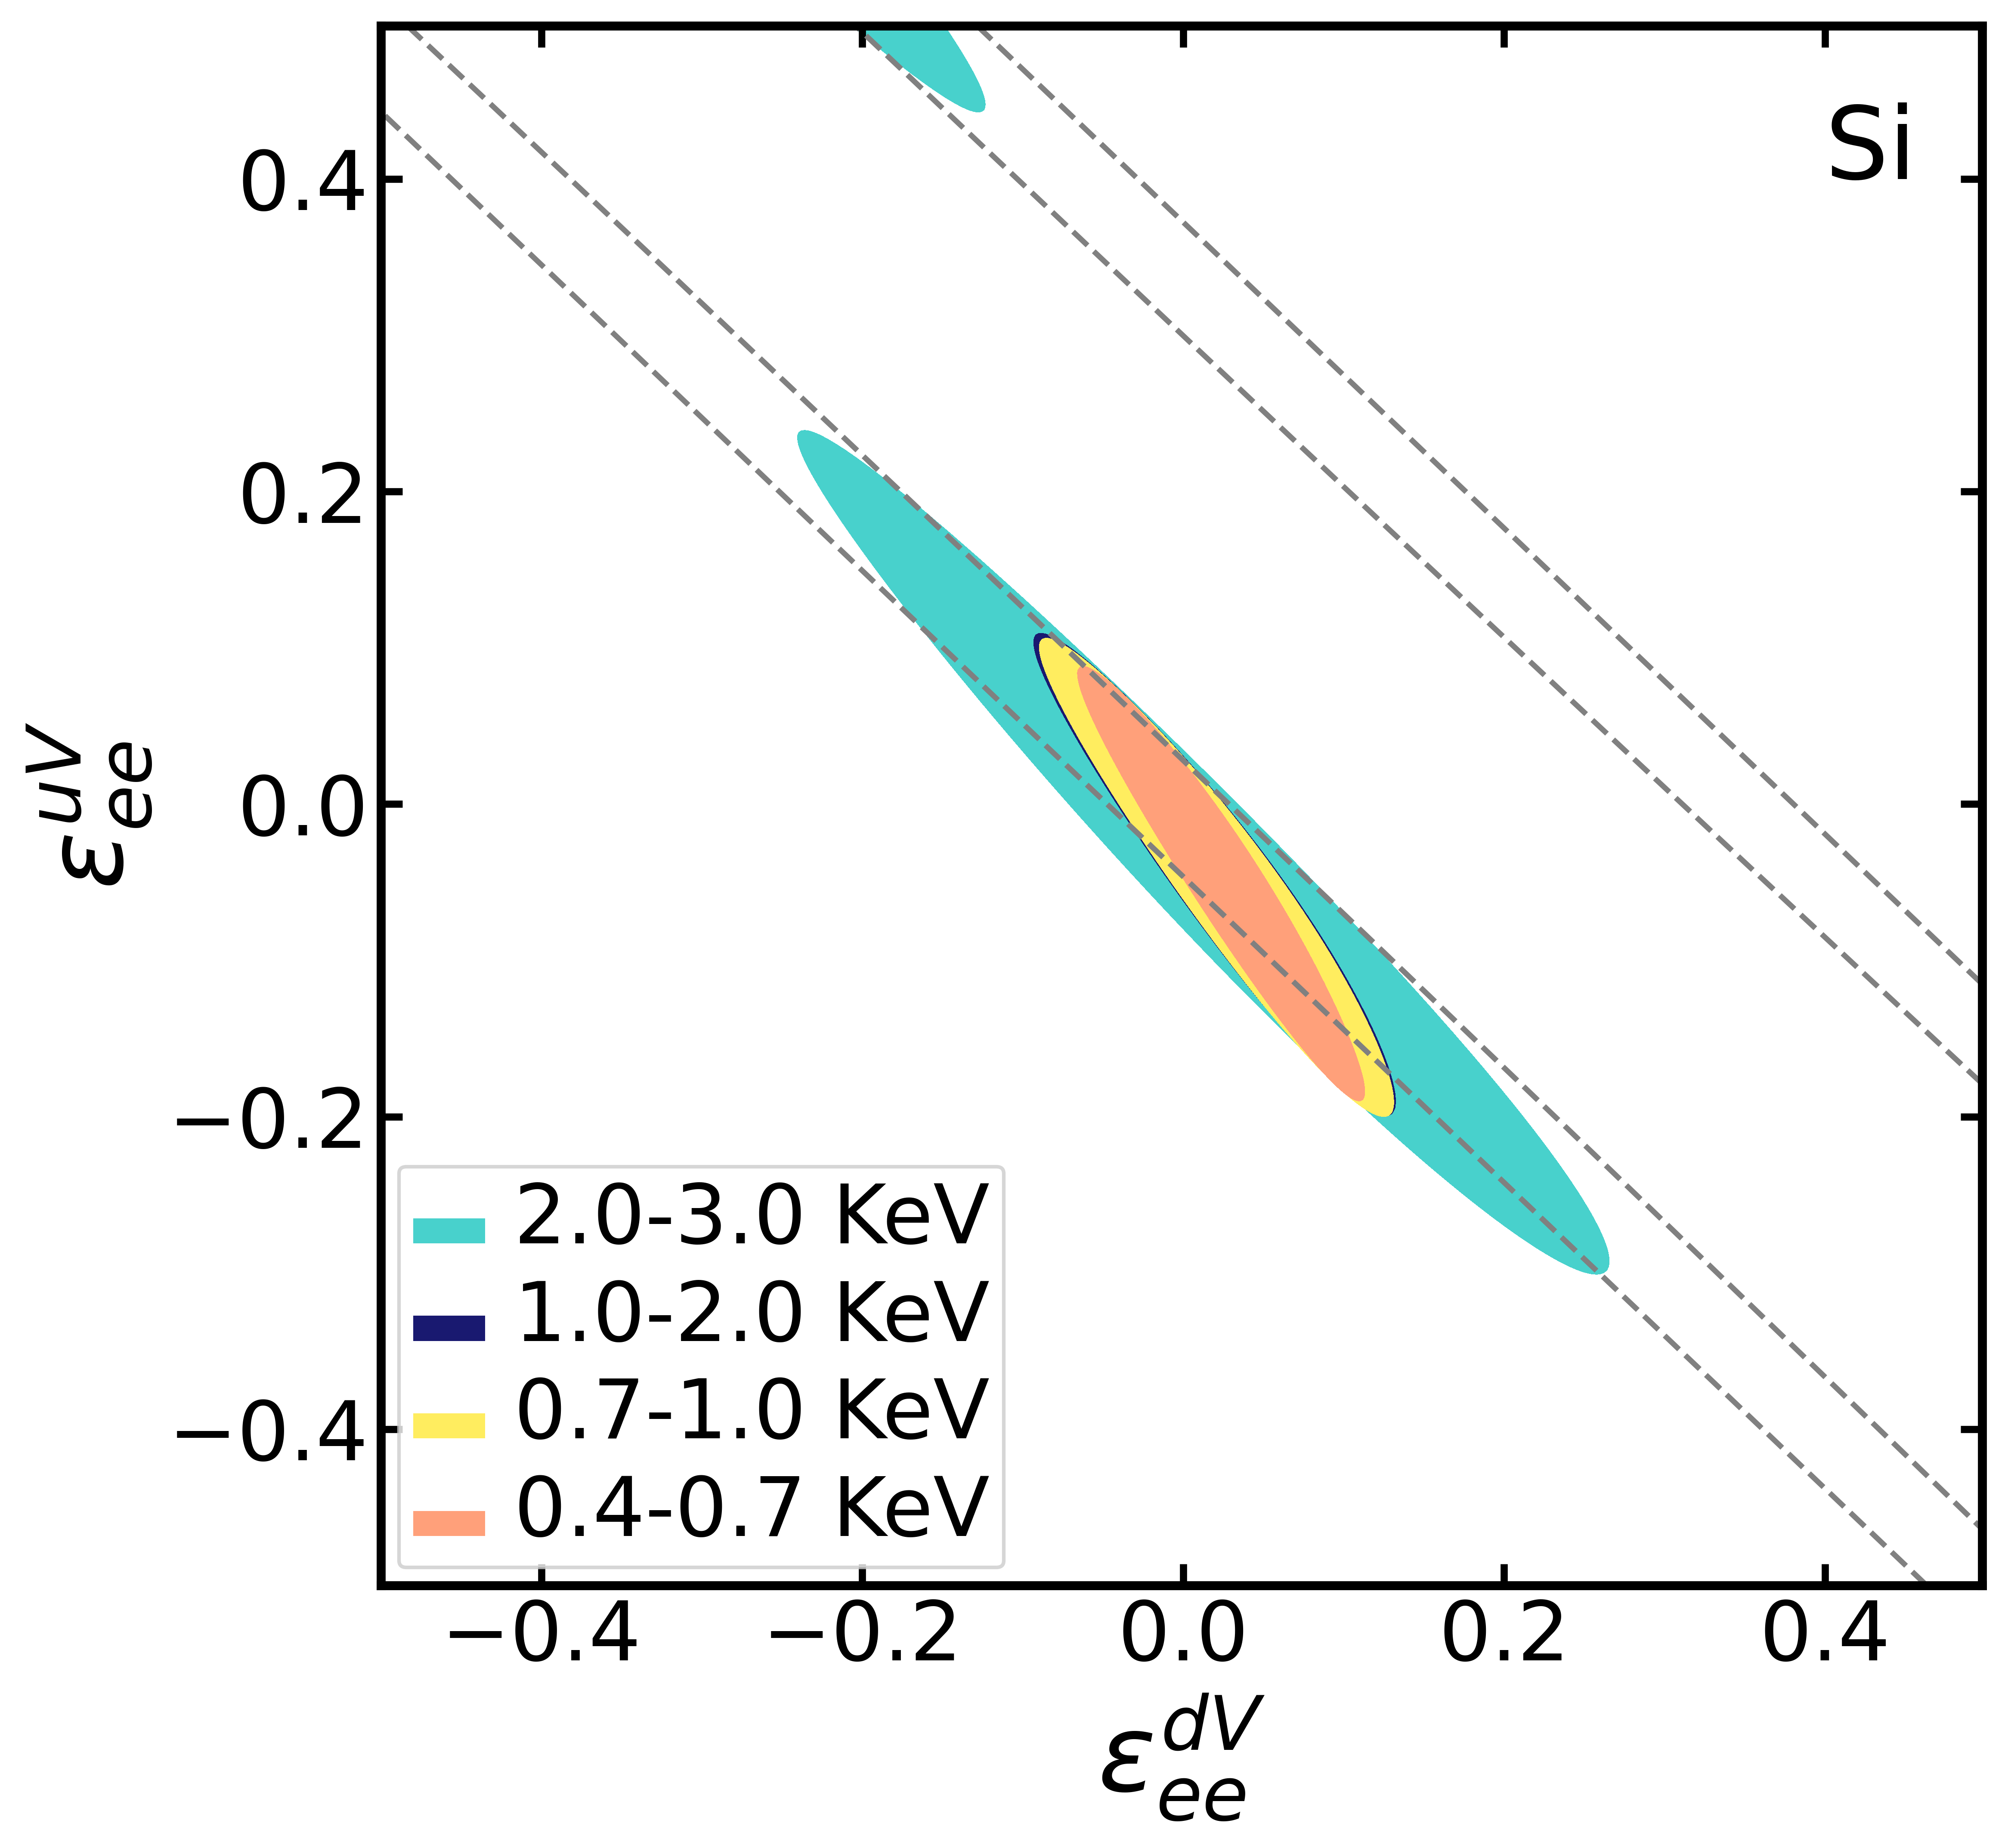
\includegraphics[scale=0.33]{figures/NSISidVu.png}}
\caption{Expected allowed values for the non-universal NSIs parameters at a 90$\%$ confidence level for the detectors exposed to reactor antineutrinos flux with different ranges of recoil energy as indicated. The left side corresponds to Zn detectors, and the right side to Si detectors. The dashed lines enclose the region corresponding to the case of uncorrelated detectors.}
\label{Reactor-NU}
\end{figure}


In itself, the reactor flux generates a large number of events for CE$\nu$NS. However, it is possible to observe that the lower the range of recoil energies considered, the higher the statistics will be; therefore, the more constrained the values. 

 Figure \ref{Reactor-FC} displays the expected allowed values for different recoil energy ranges for the flavor-changing parameter $\varepsilon_{\tau e}^{dV}$ versus the non-universal parameter $\varepsilon_{ee}^{dV}$. This time, two cases were analyzed: one with systematic errors of $\sigma_A=25\%$ and $\sigma_B=10\%$ and another with the ideal case of systematic errors of $\sigma_A=\sigma_B=5\%$. As expected, the second case exhibits better sensitivity to the parameter values. 
\begin{figure}[h!]
\centering
\subfigure{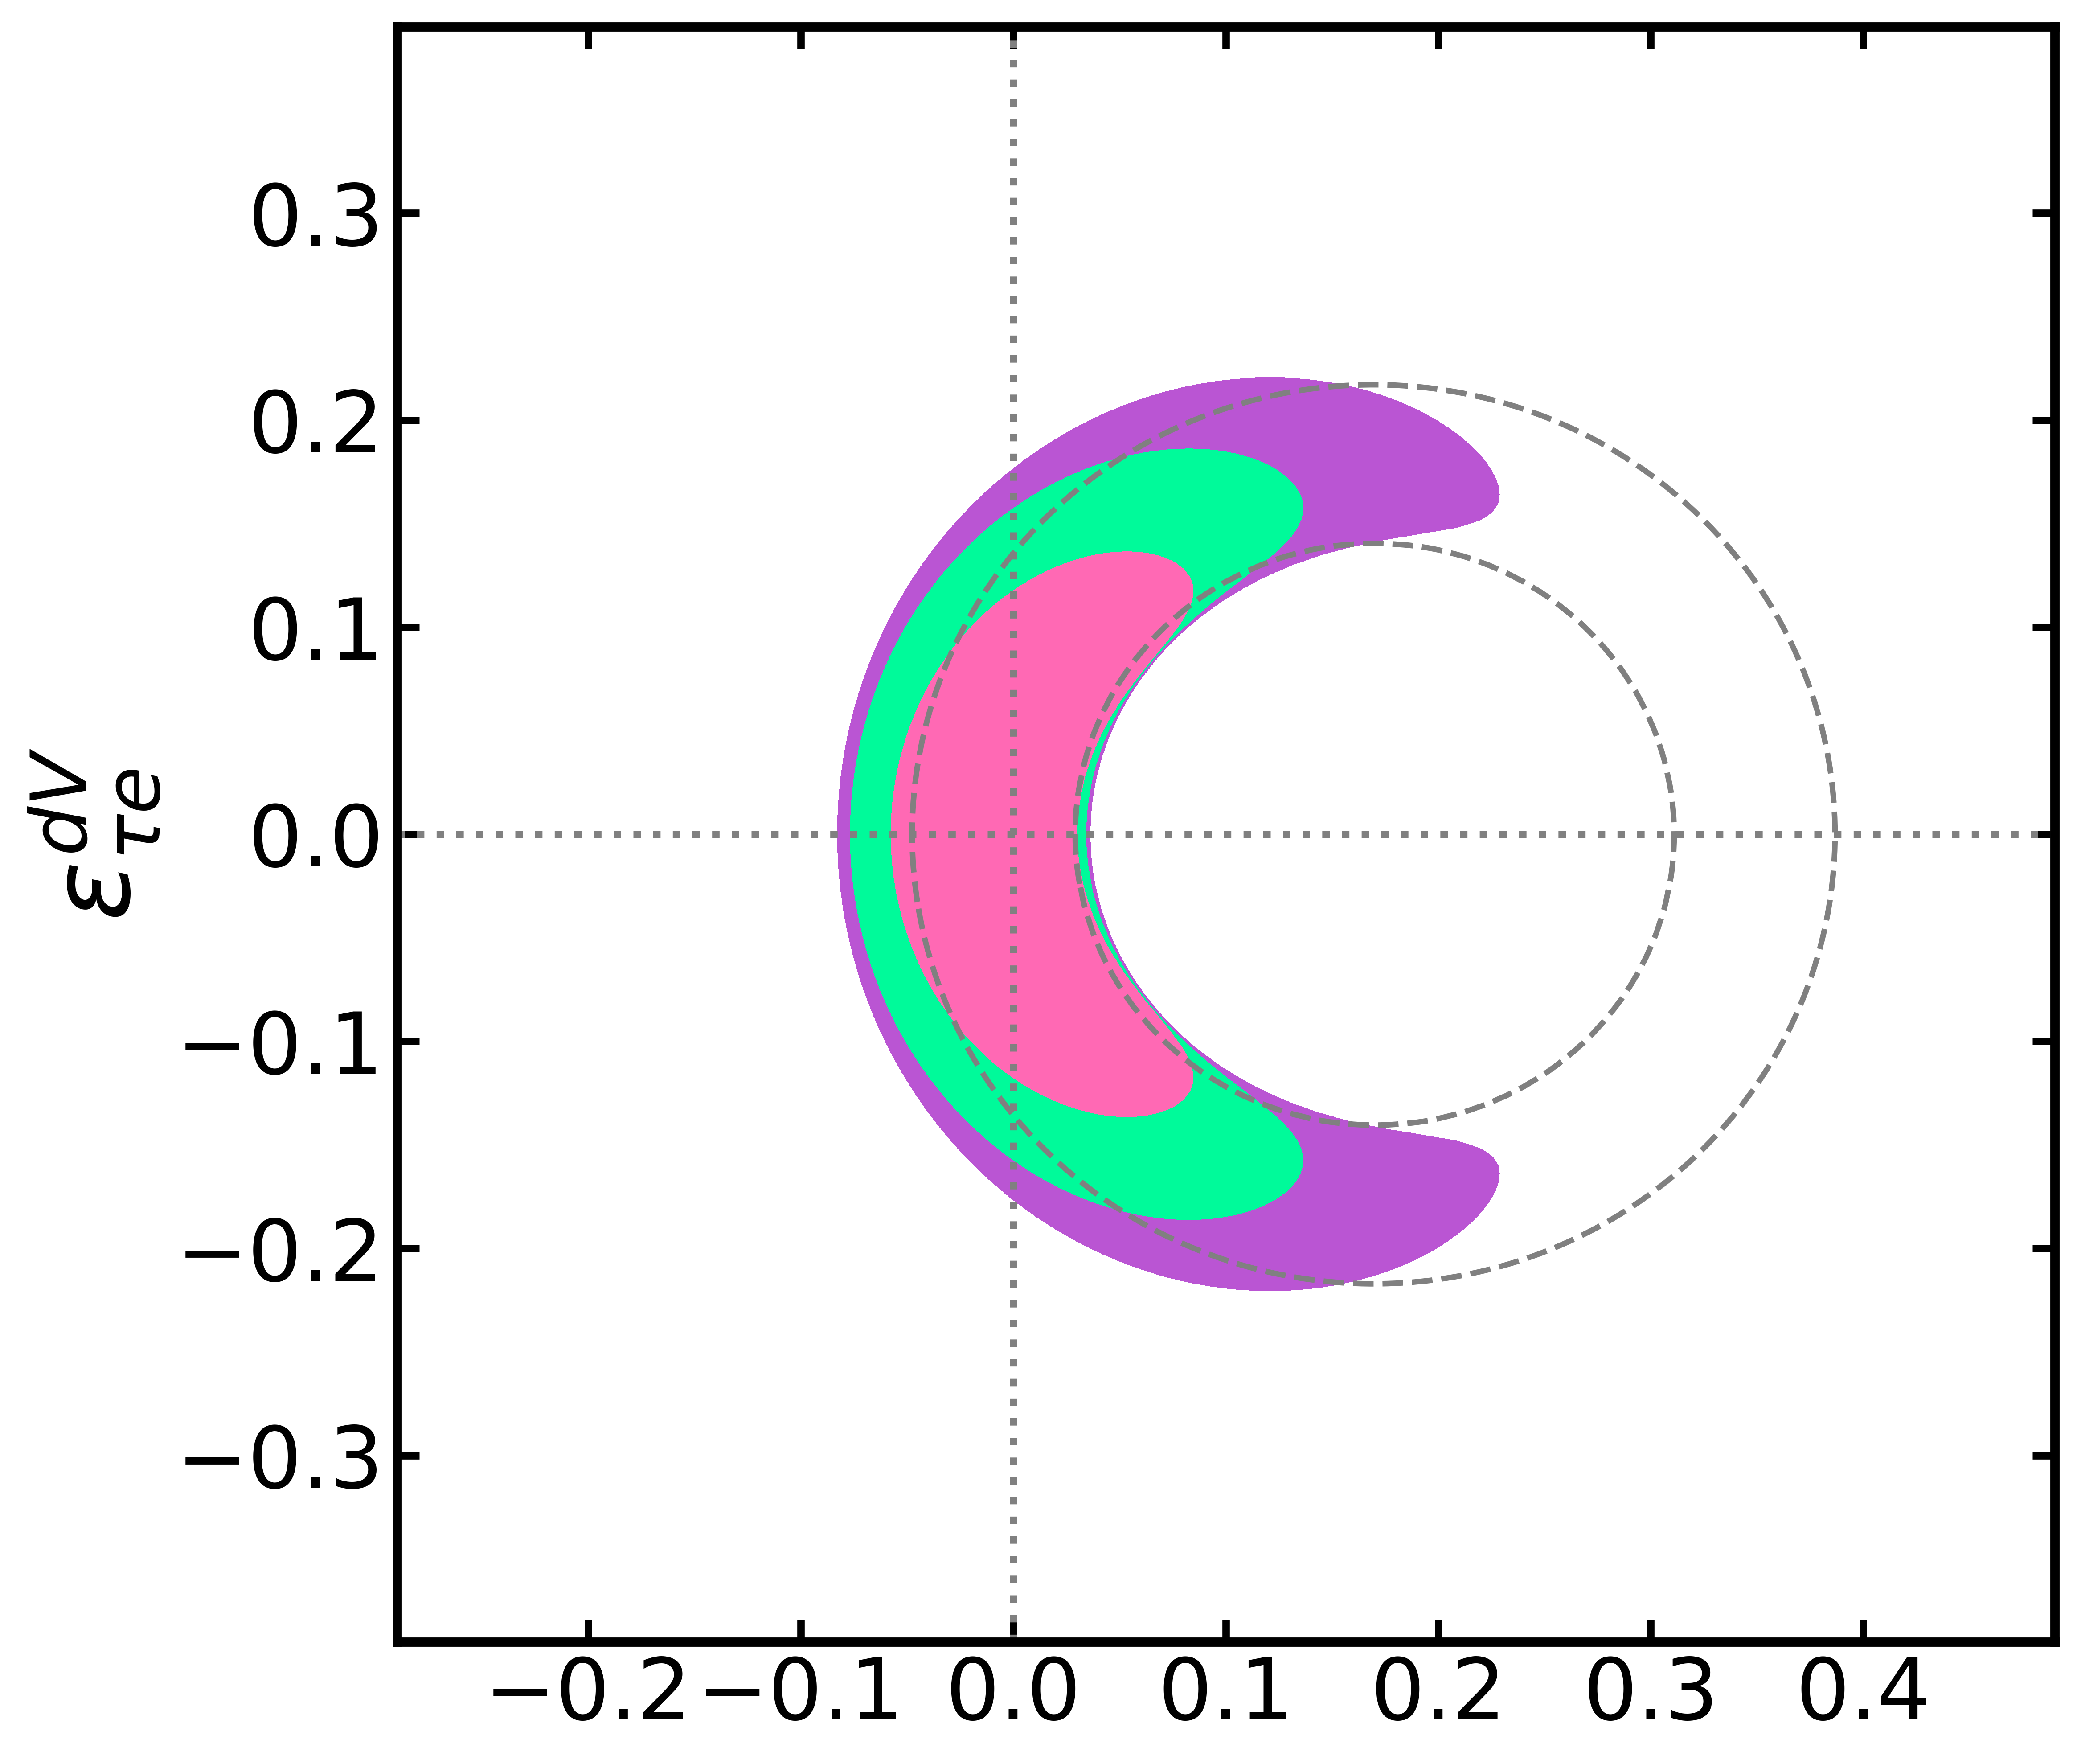
\includegraphics[scale=0.33]{figures/NSIZn25Emu.png}}\hspace{0.5em}%
\subfigure{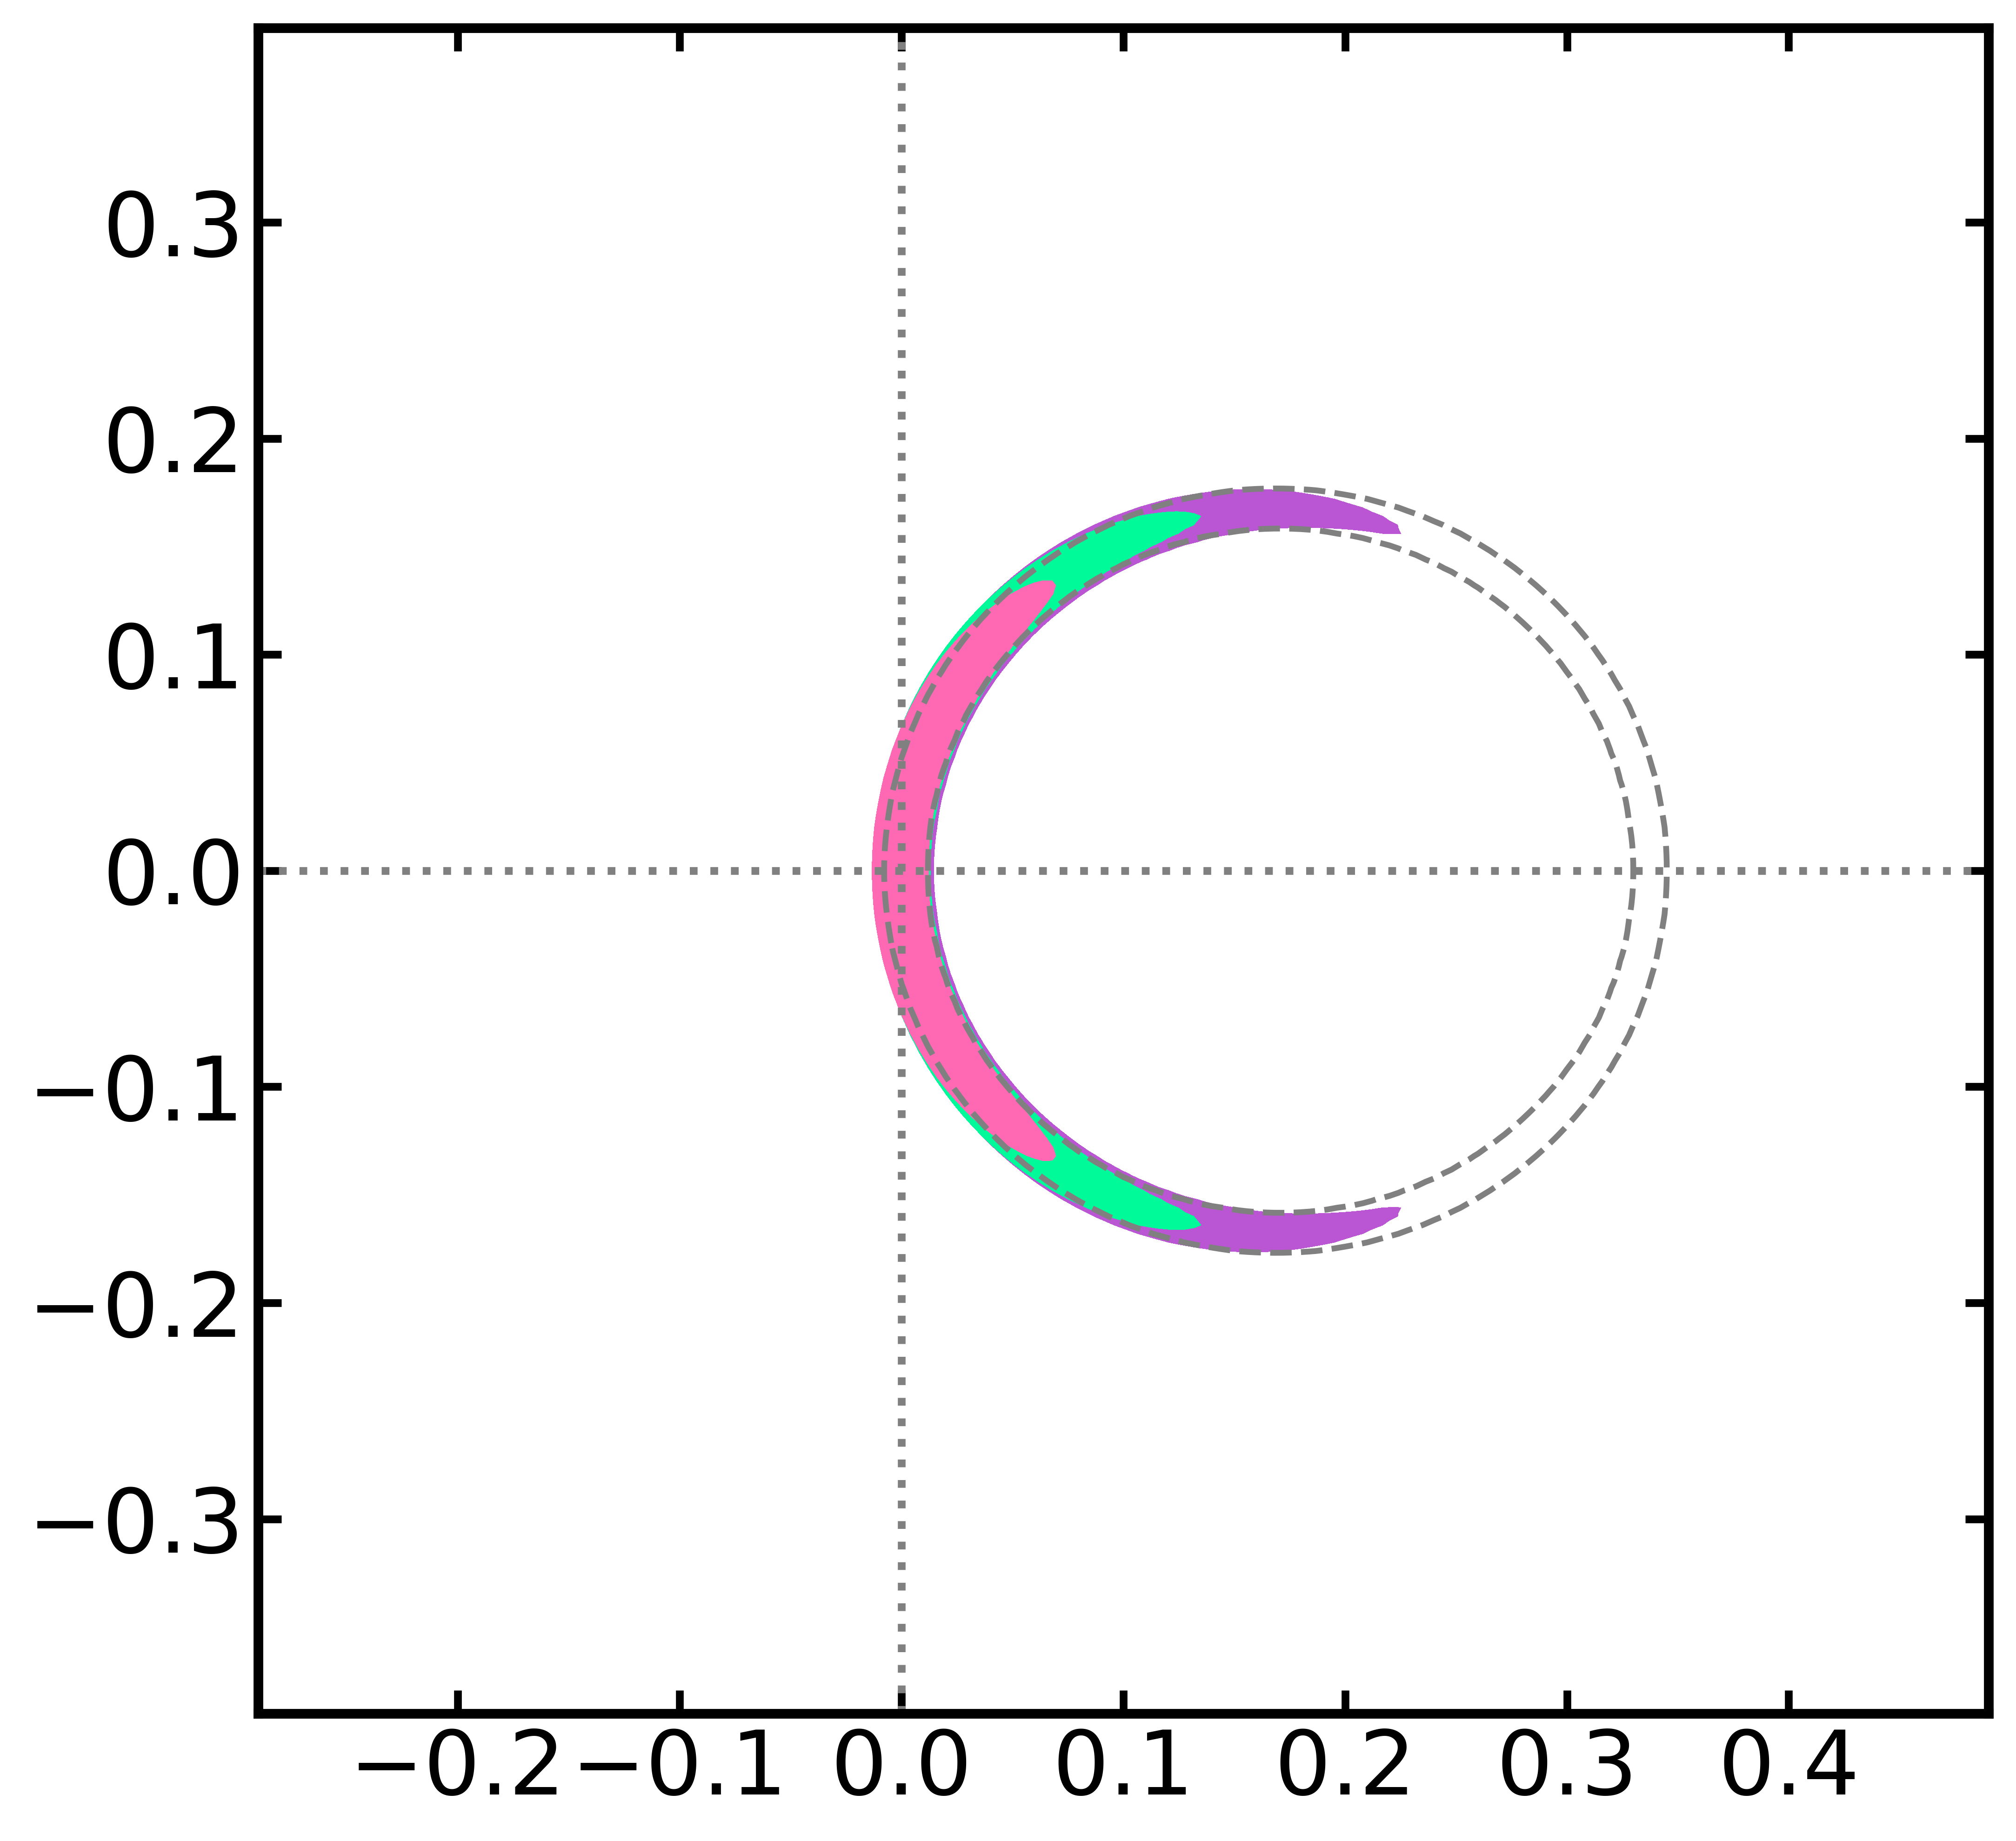
\includegraphics[scale=0.33]{figures/NSIZn5Emu.png}}\par \vspace{0.5em}
\subfigure{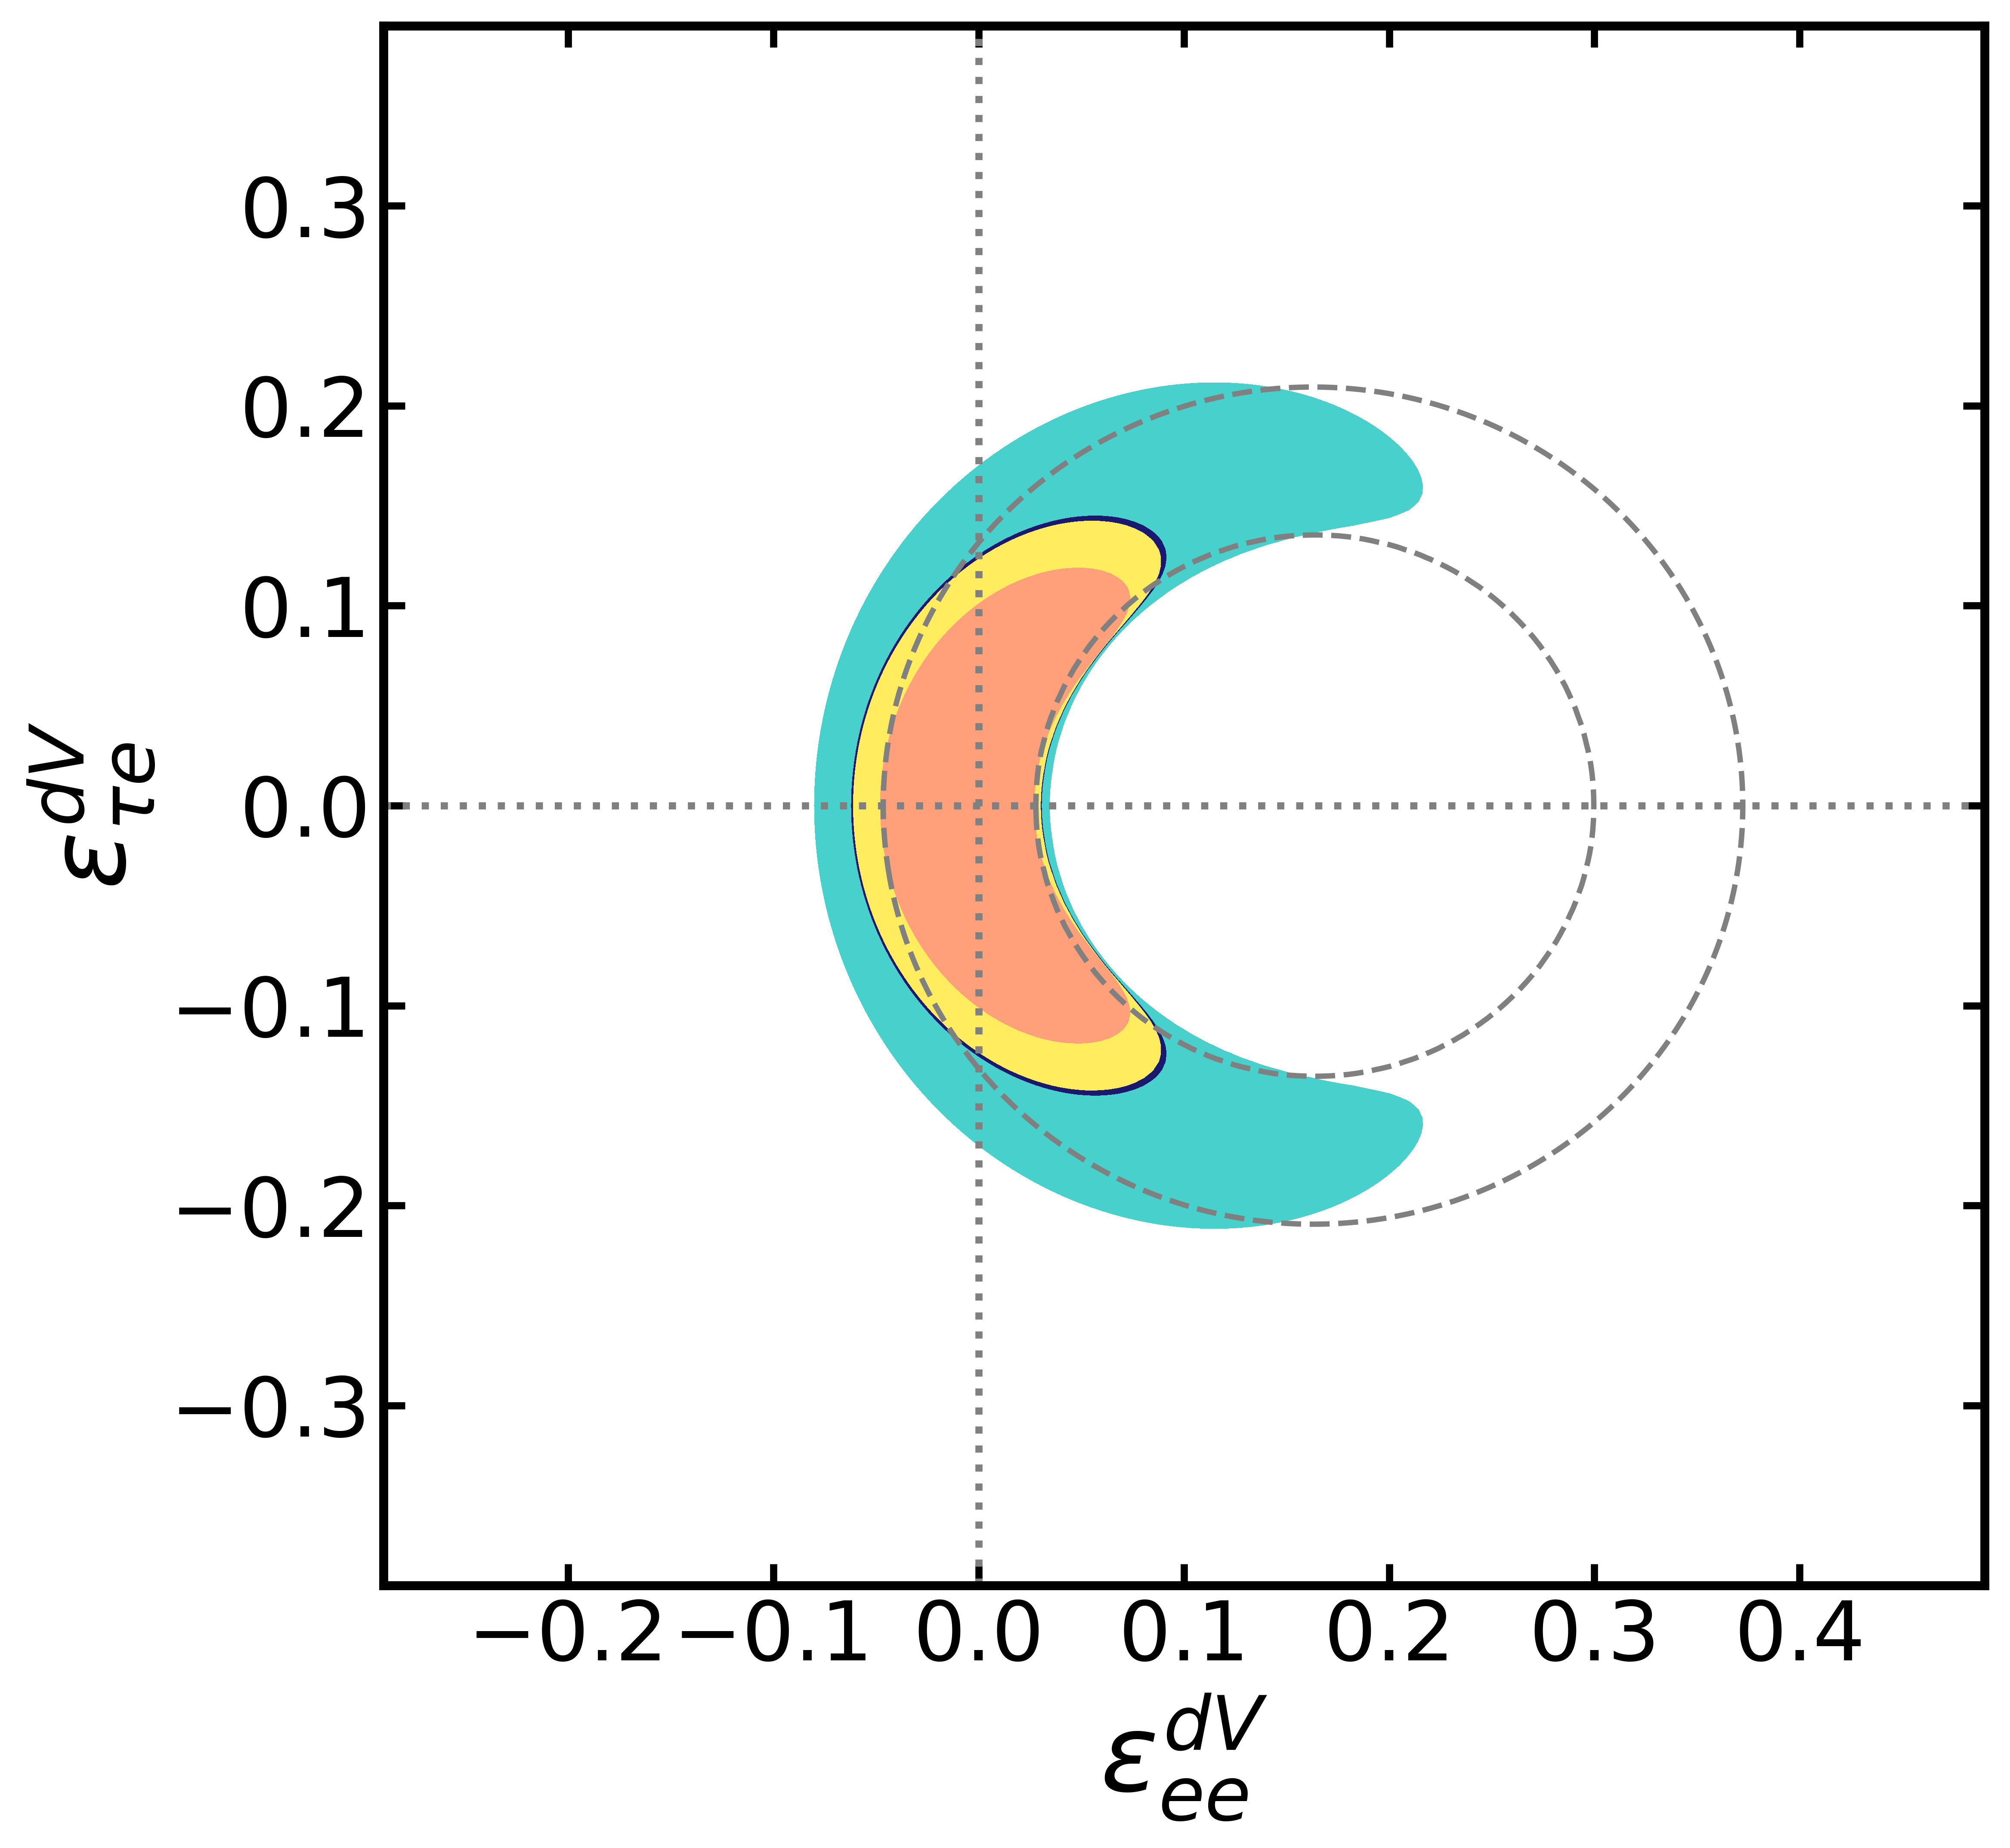
\includegraphics[scale=0.33]{figures/NSISi25Emu.png}}\hspace{0.5em}%
\subfigure{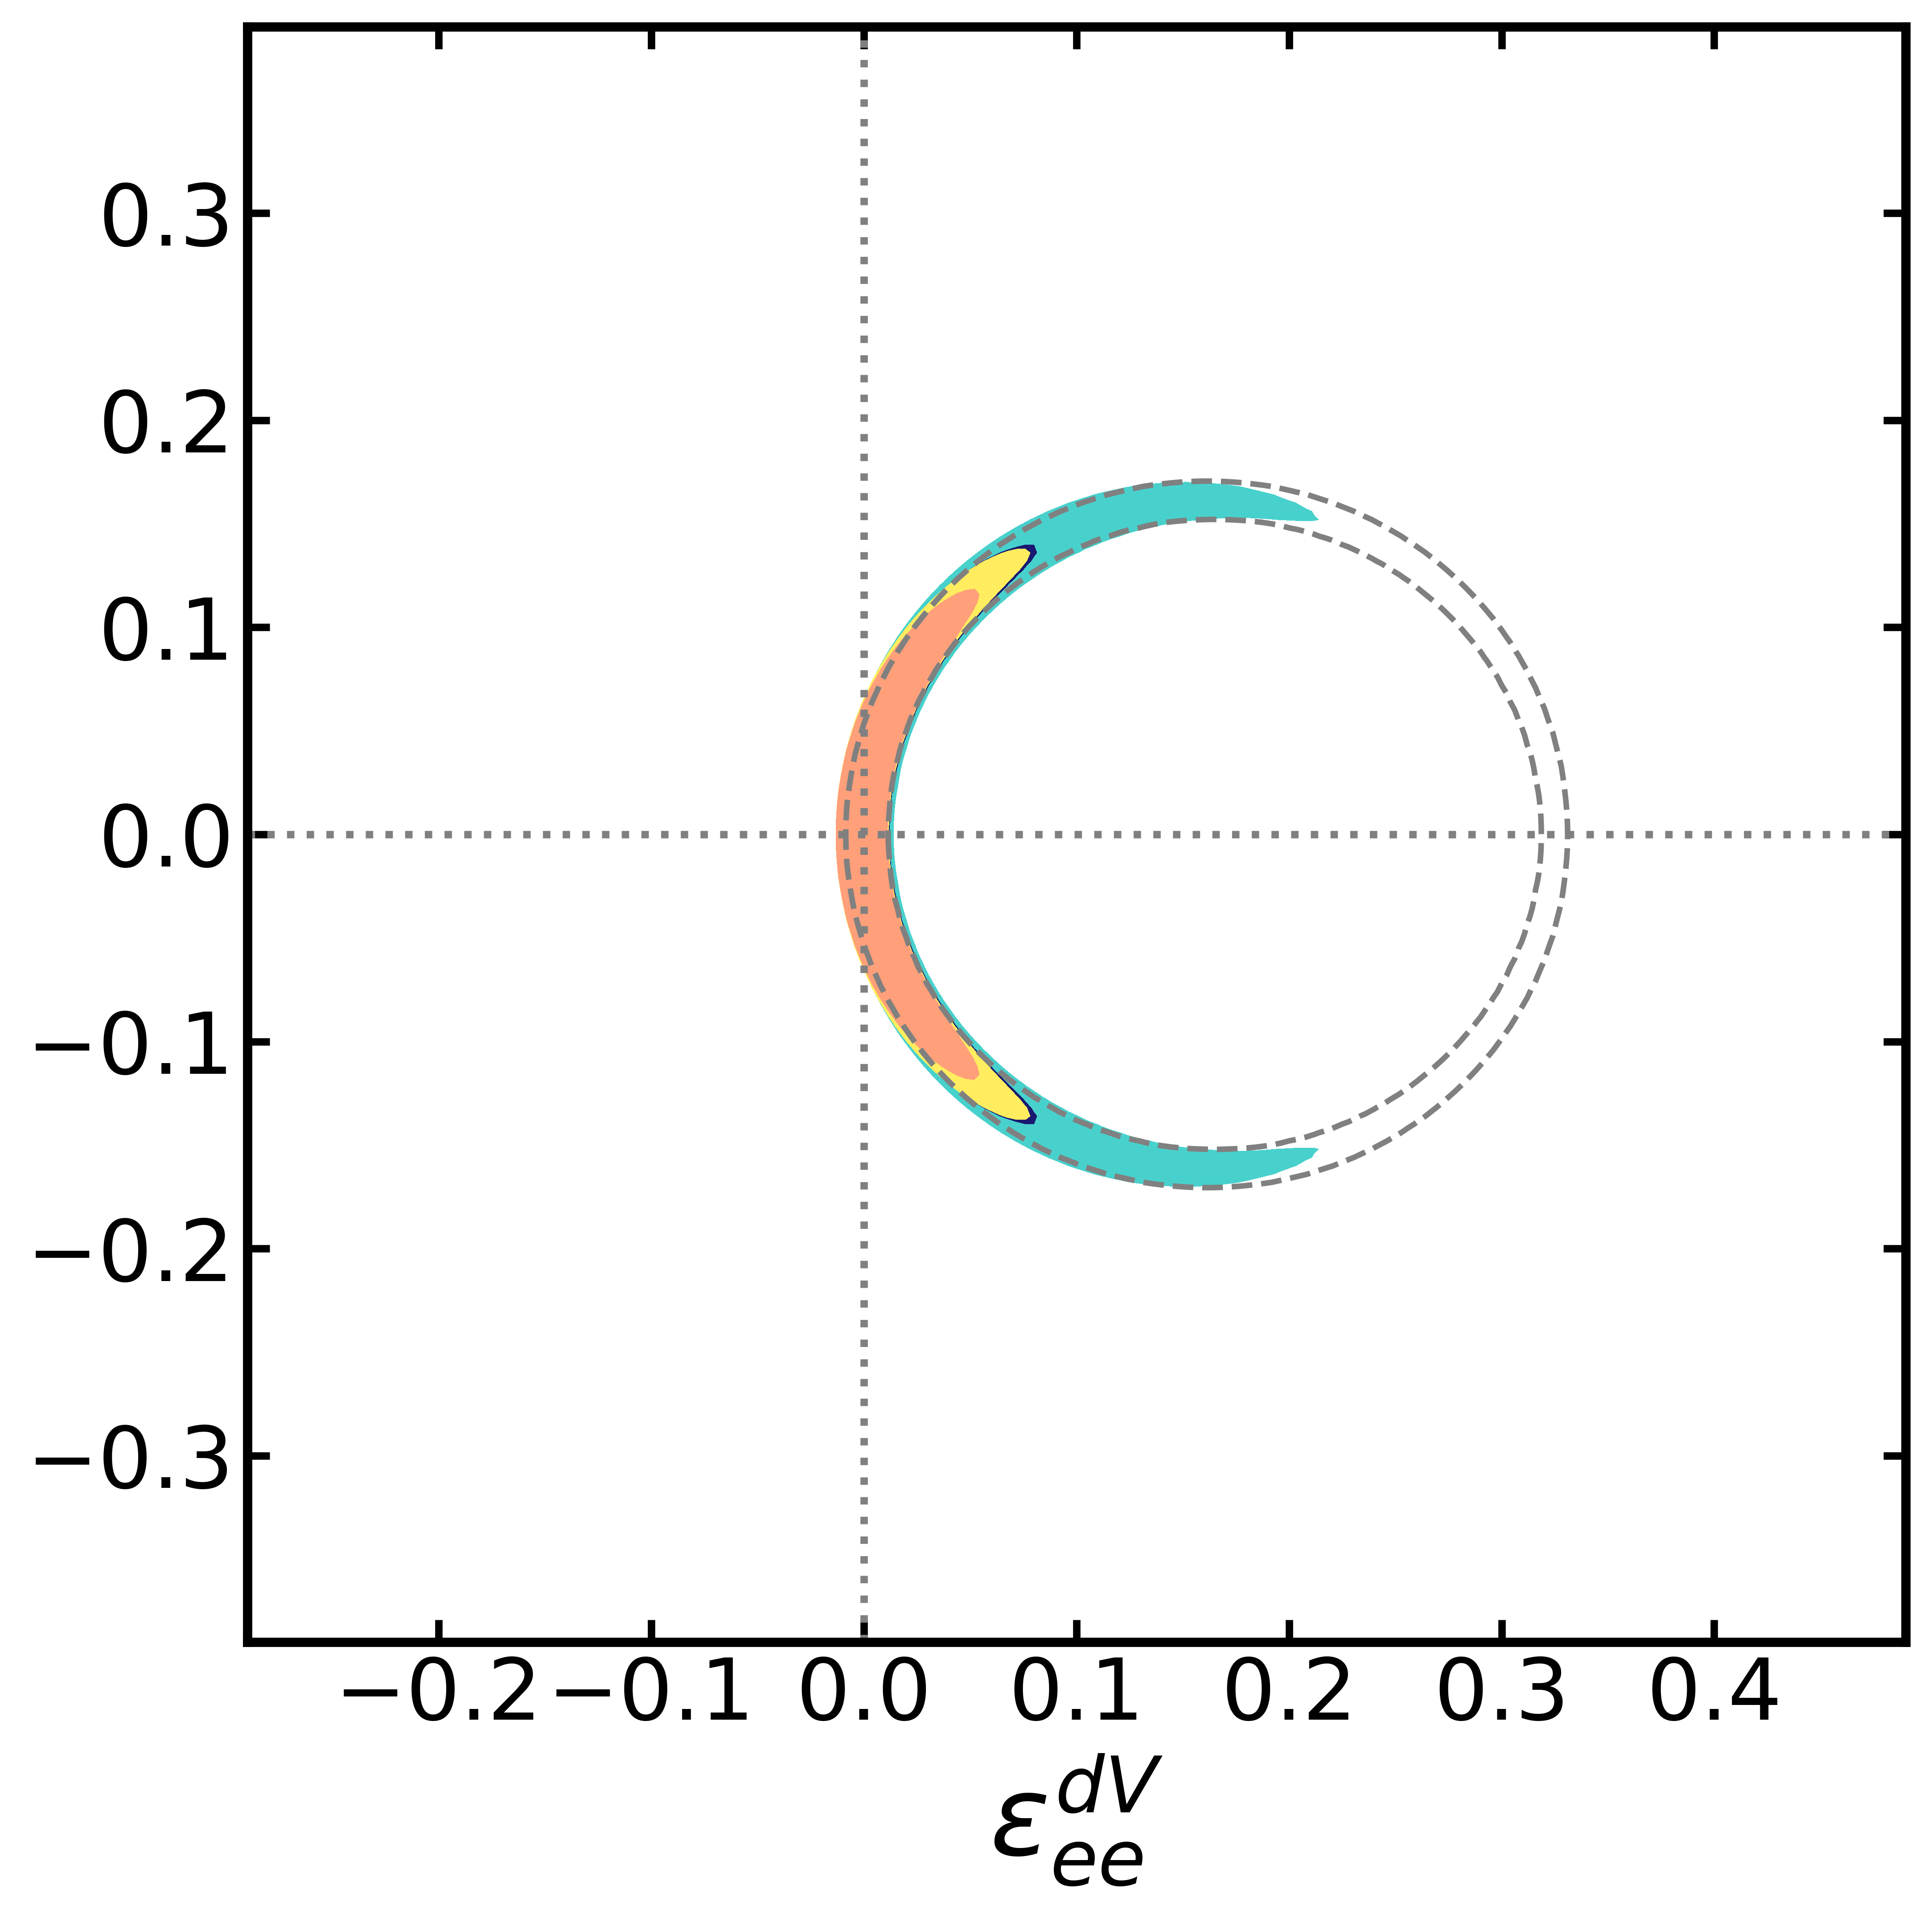
\includegraphics[scale=0.33]{figures/NSISi5Emu.png}}
\caption{Expected allowed values for the flavor changing $\varepsilon_{\tau e}^{dV}$ vs the non-universal $\varepsilon_{ee}^{dV}$ NSIs parameters at a 90$\%$ confidence level for the detectors exposed to a reactor antineutrino flux with different ranges of recoil energy as indicated. The upper panel corresponds to Zn detectors, and the lower panel corresponds to Si detectors. The left side refers to the case of $\sigma_A=25\%$ and $\sigma_B=10\%$ while the right side refers to the case of $\sigma_A=\sigma_B=5\%$. Also, the dashed lines enclose the region corresponding to the case of uncorrelated detectors.}
\label{Reactor-FC}
\end{figure}
\newpage
Additionally, it can be observed that, once again, the correlation between detectors breaks the degeneracy previously observed.


\begin{figure}[h!]
\centering
\subfigure{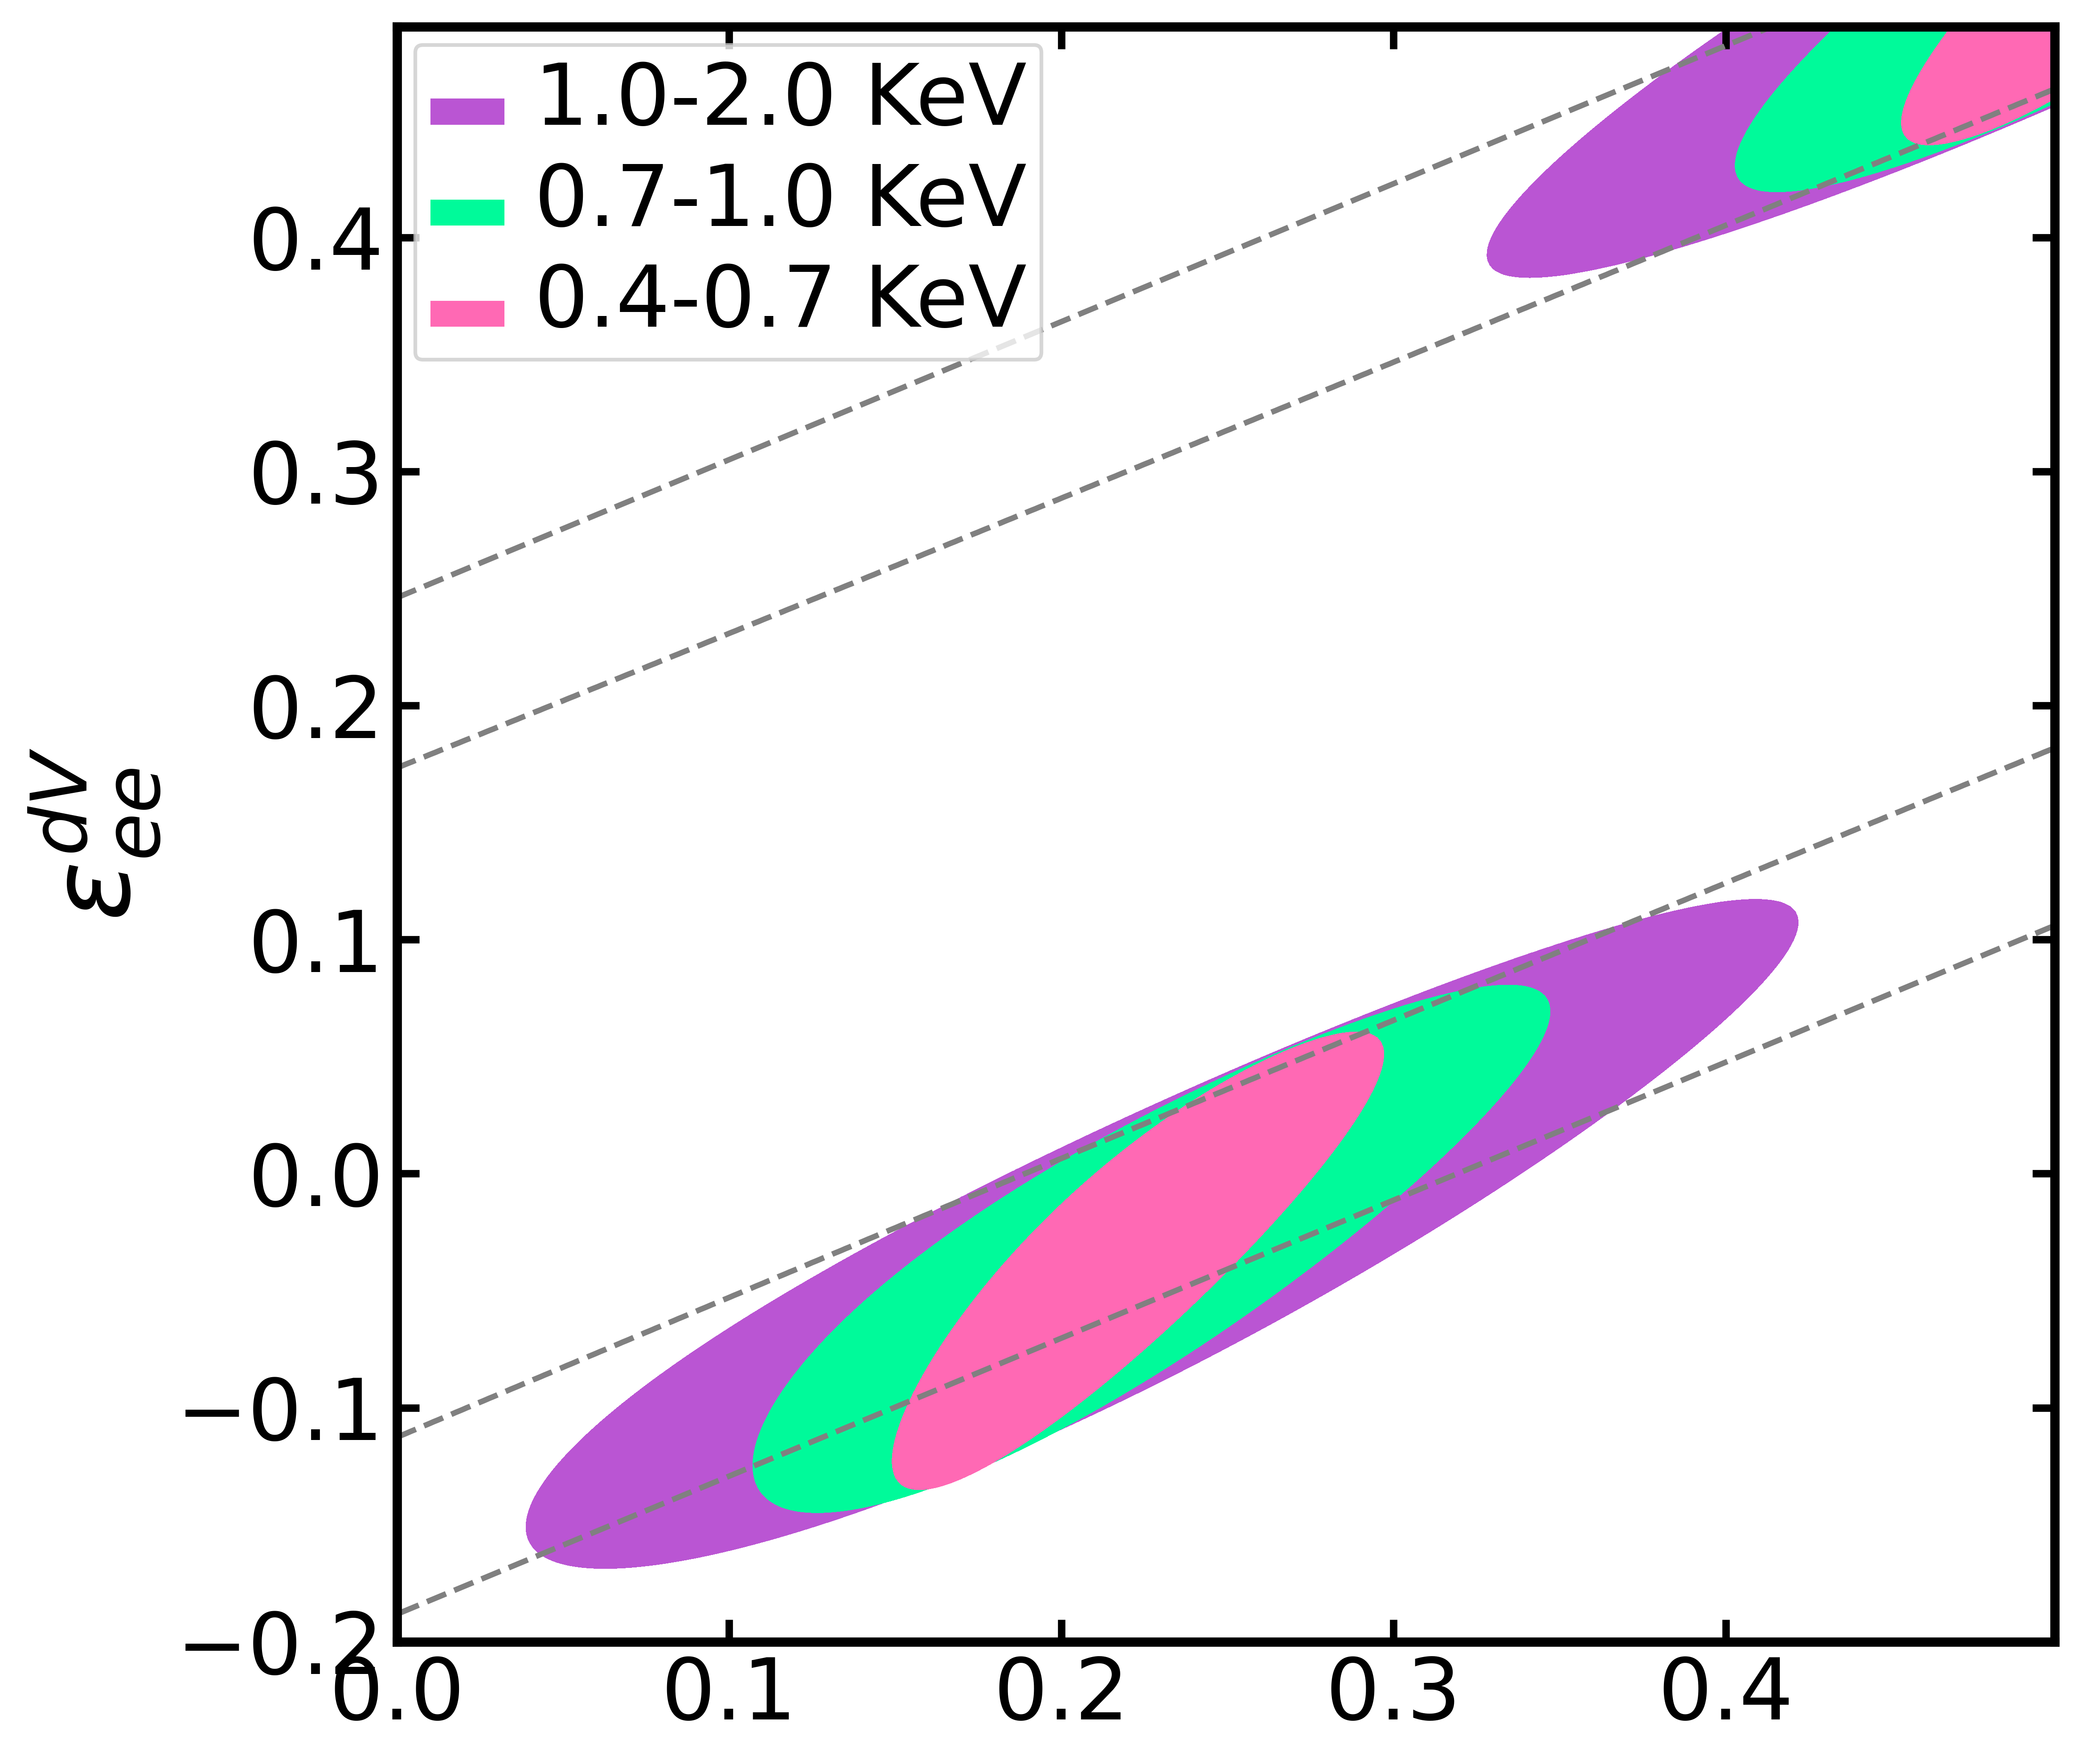
\includegraphics[scale=0.283]{figures/NSIZn25.png}}\hspace{0em}%
\subfigure{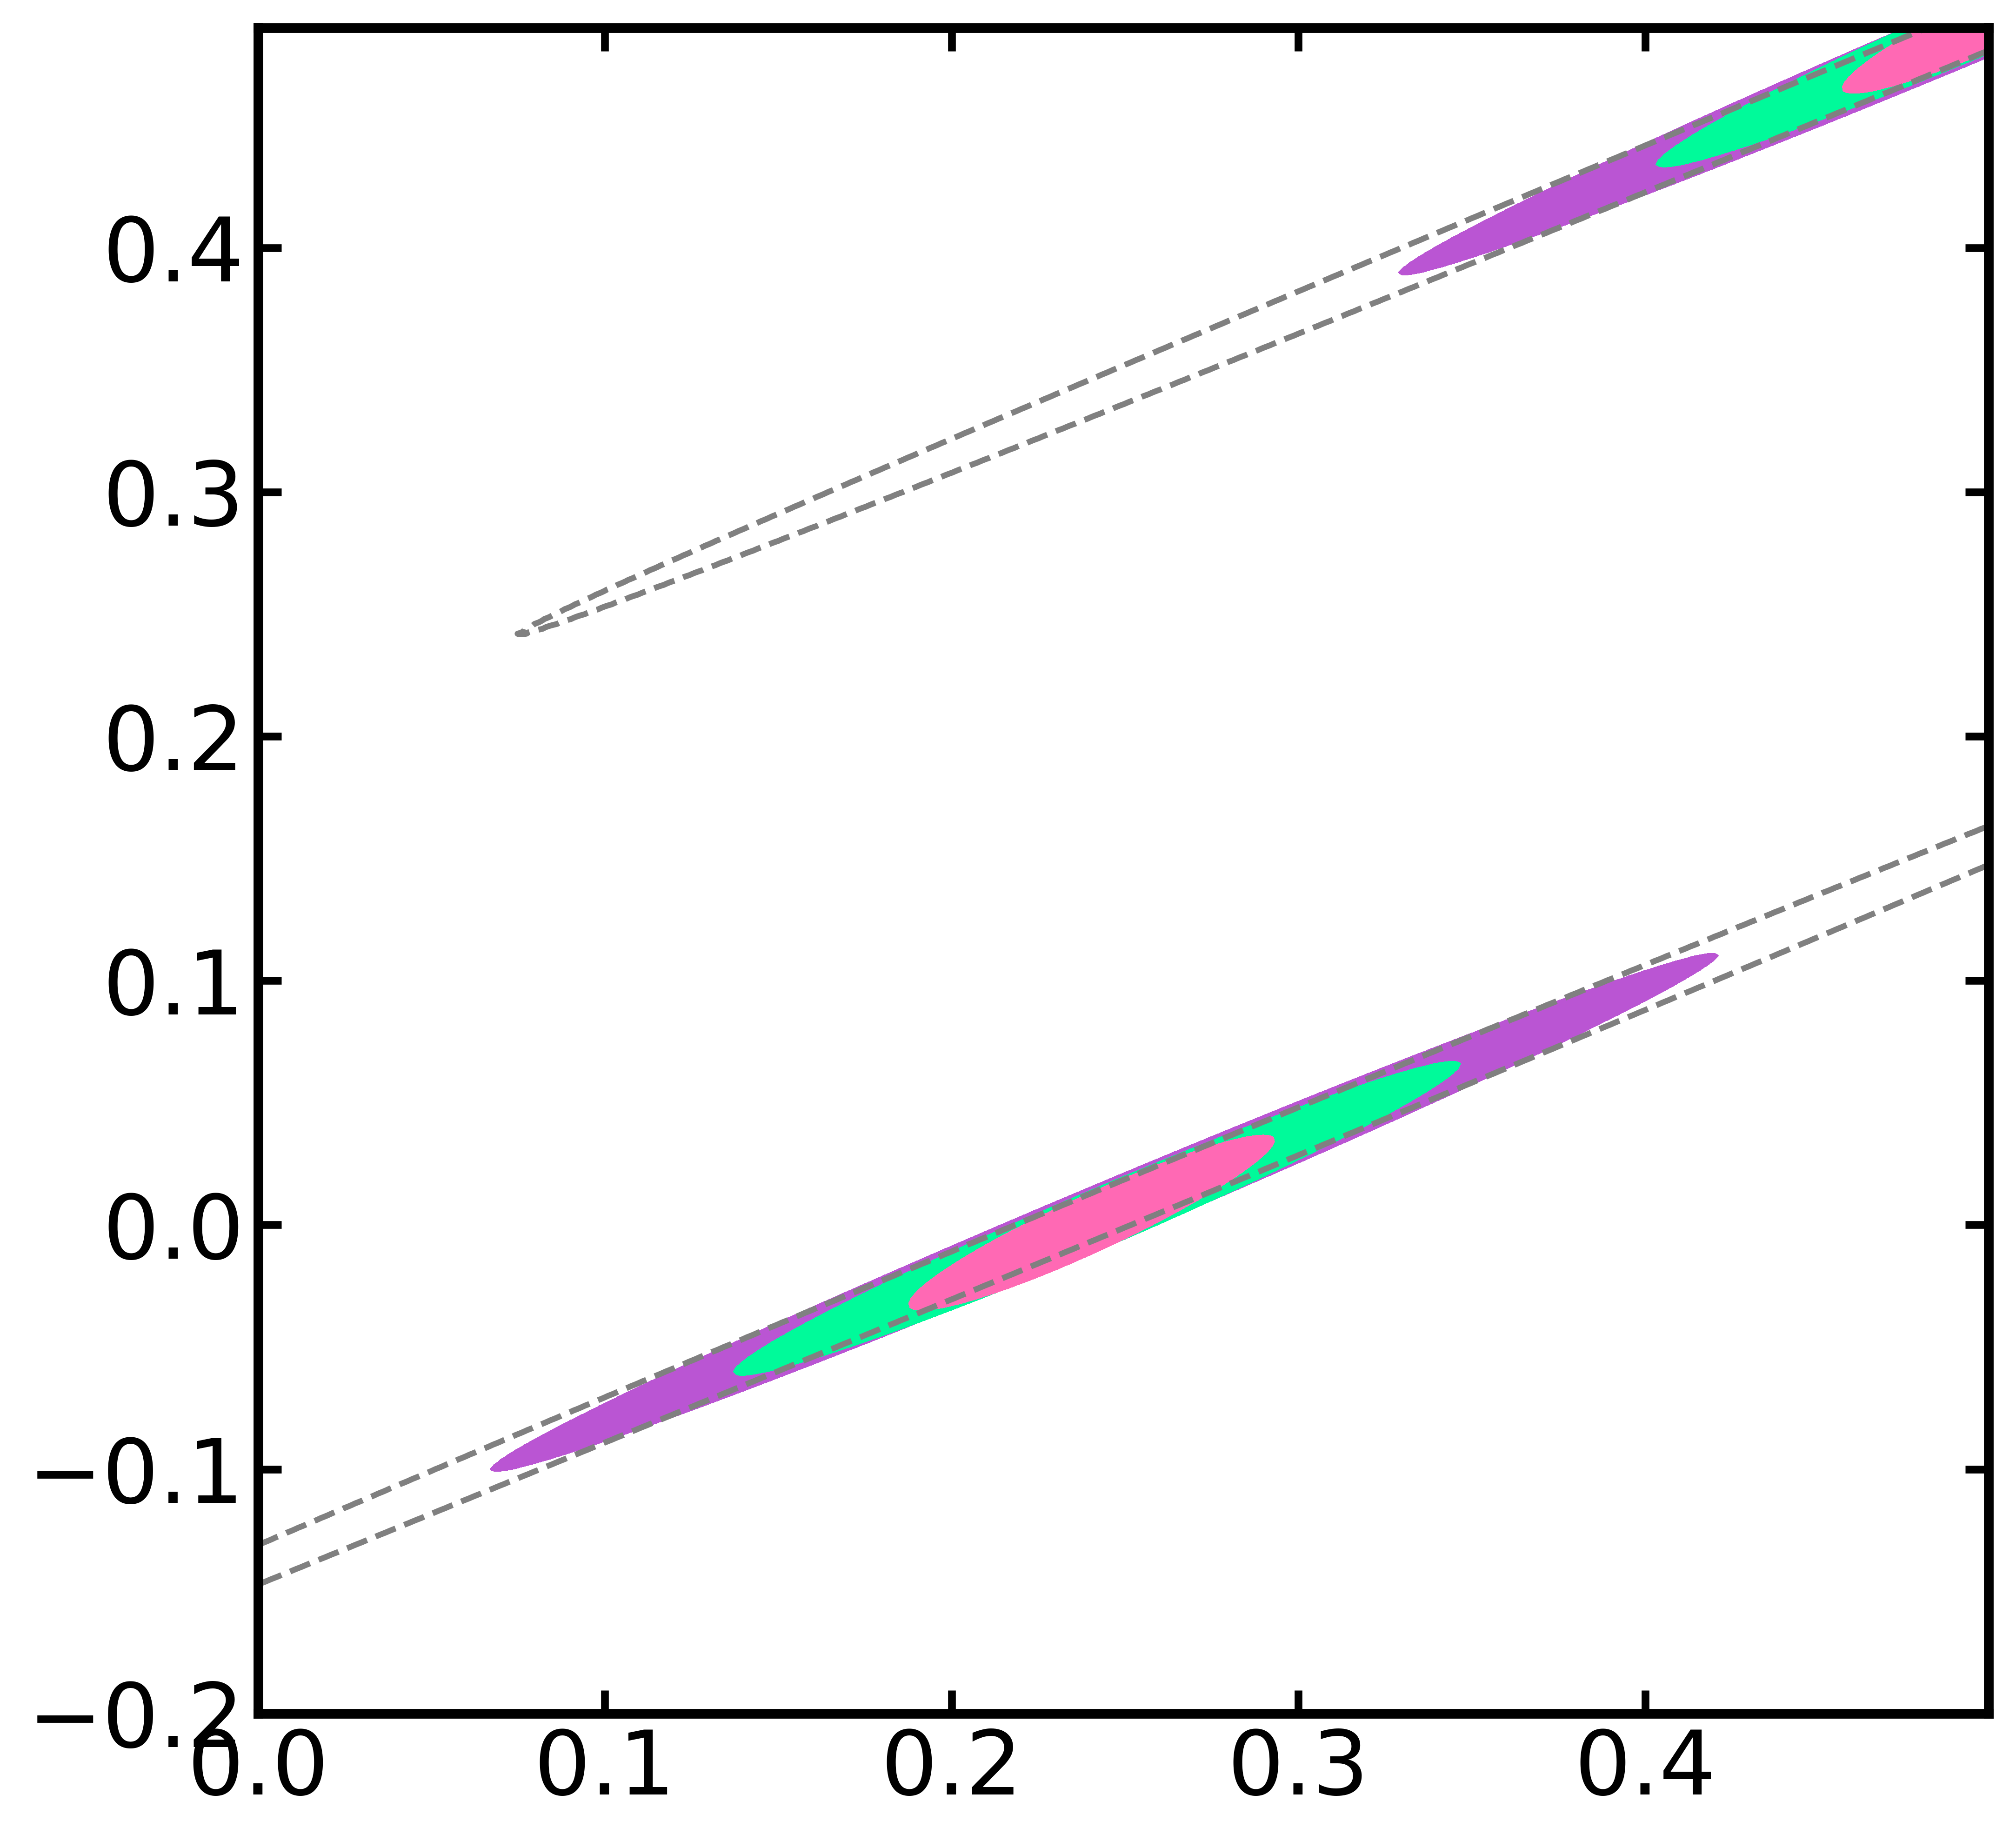
\includegraphics[scale=0.283]{figures/NSIZn5.png}}\hspace{0em}%
\subfigure{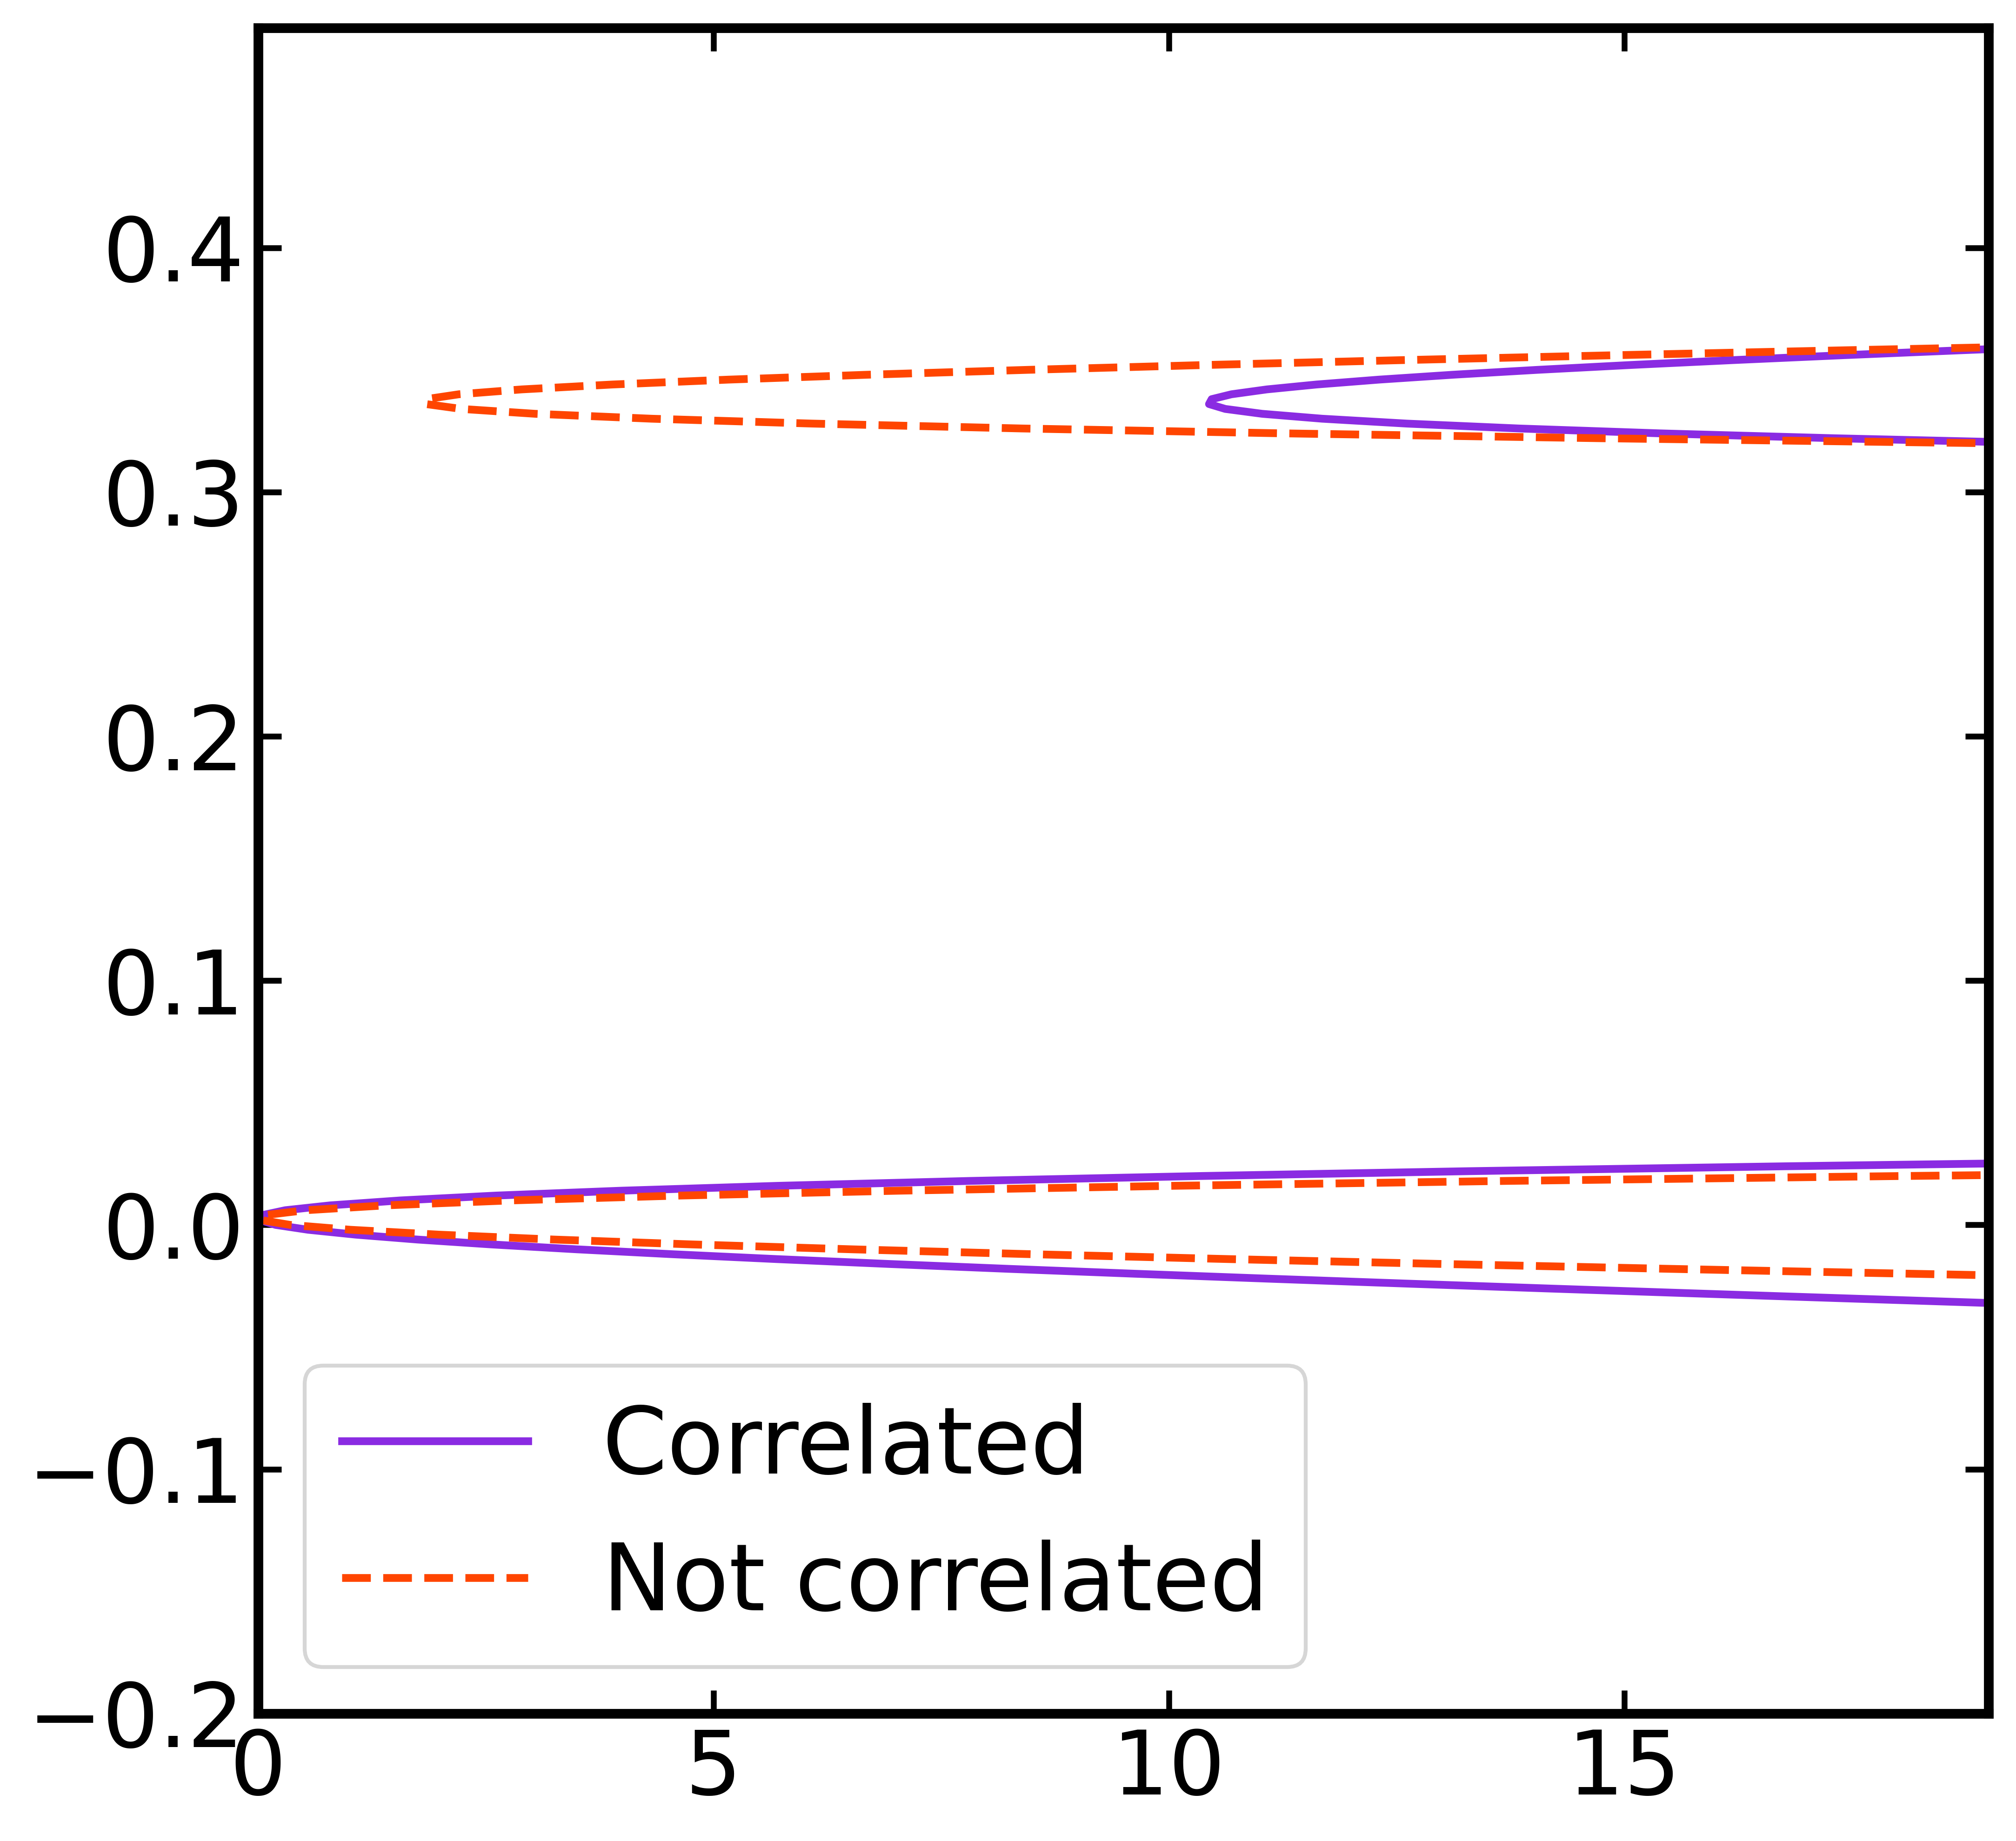
\includegraphics[scale=0.283]{figures/EeedVZn.png}}\par \vspace{-0.5em}
\subfigure{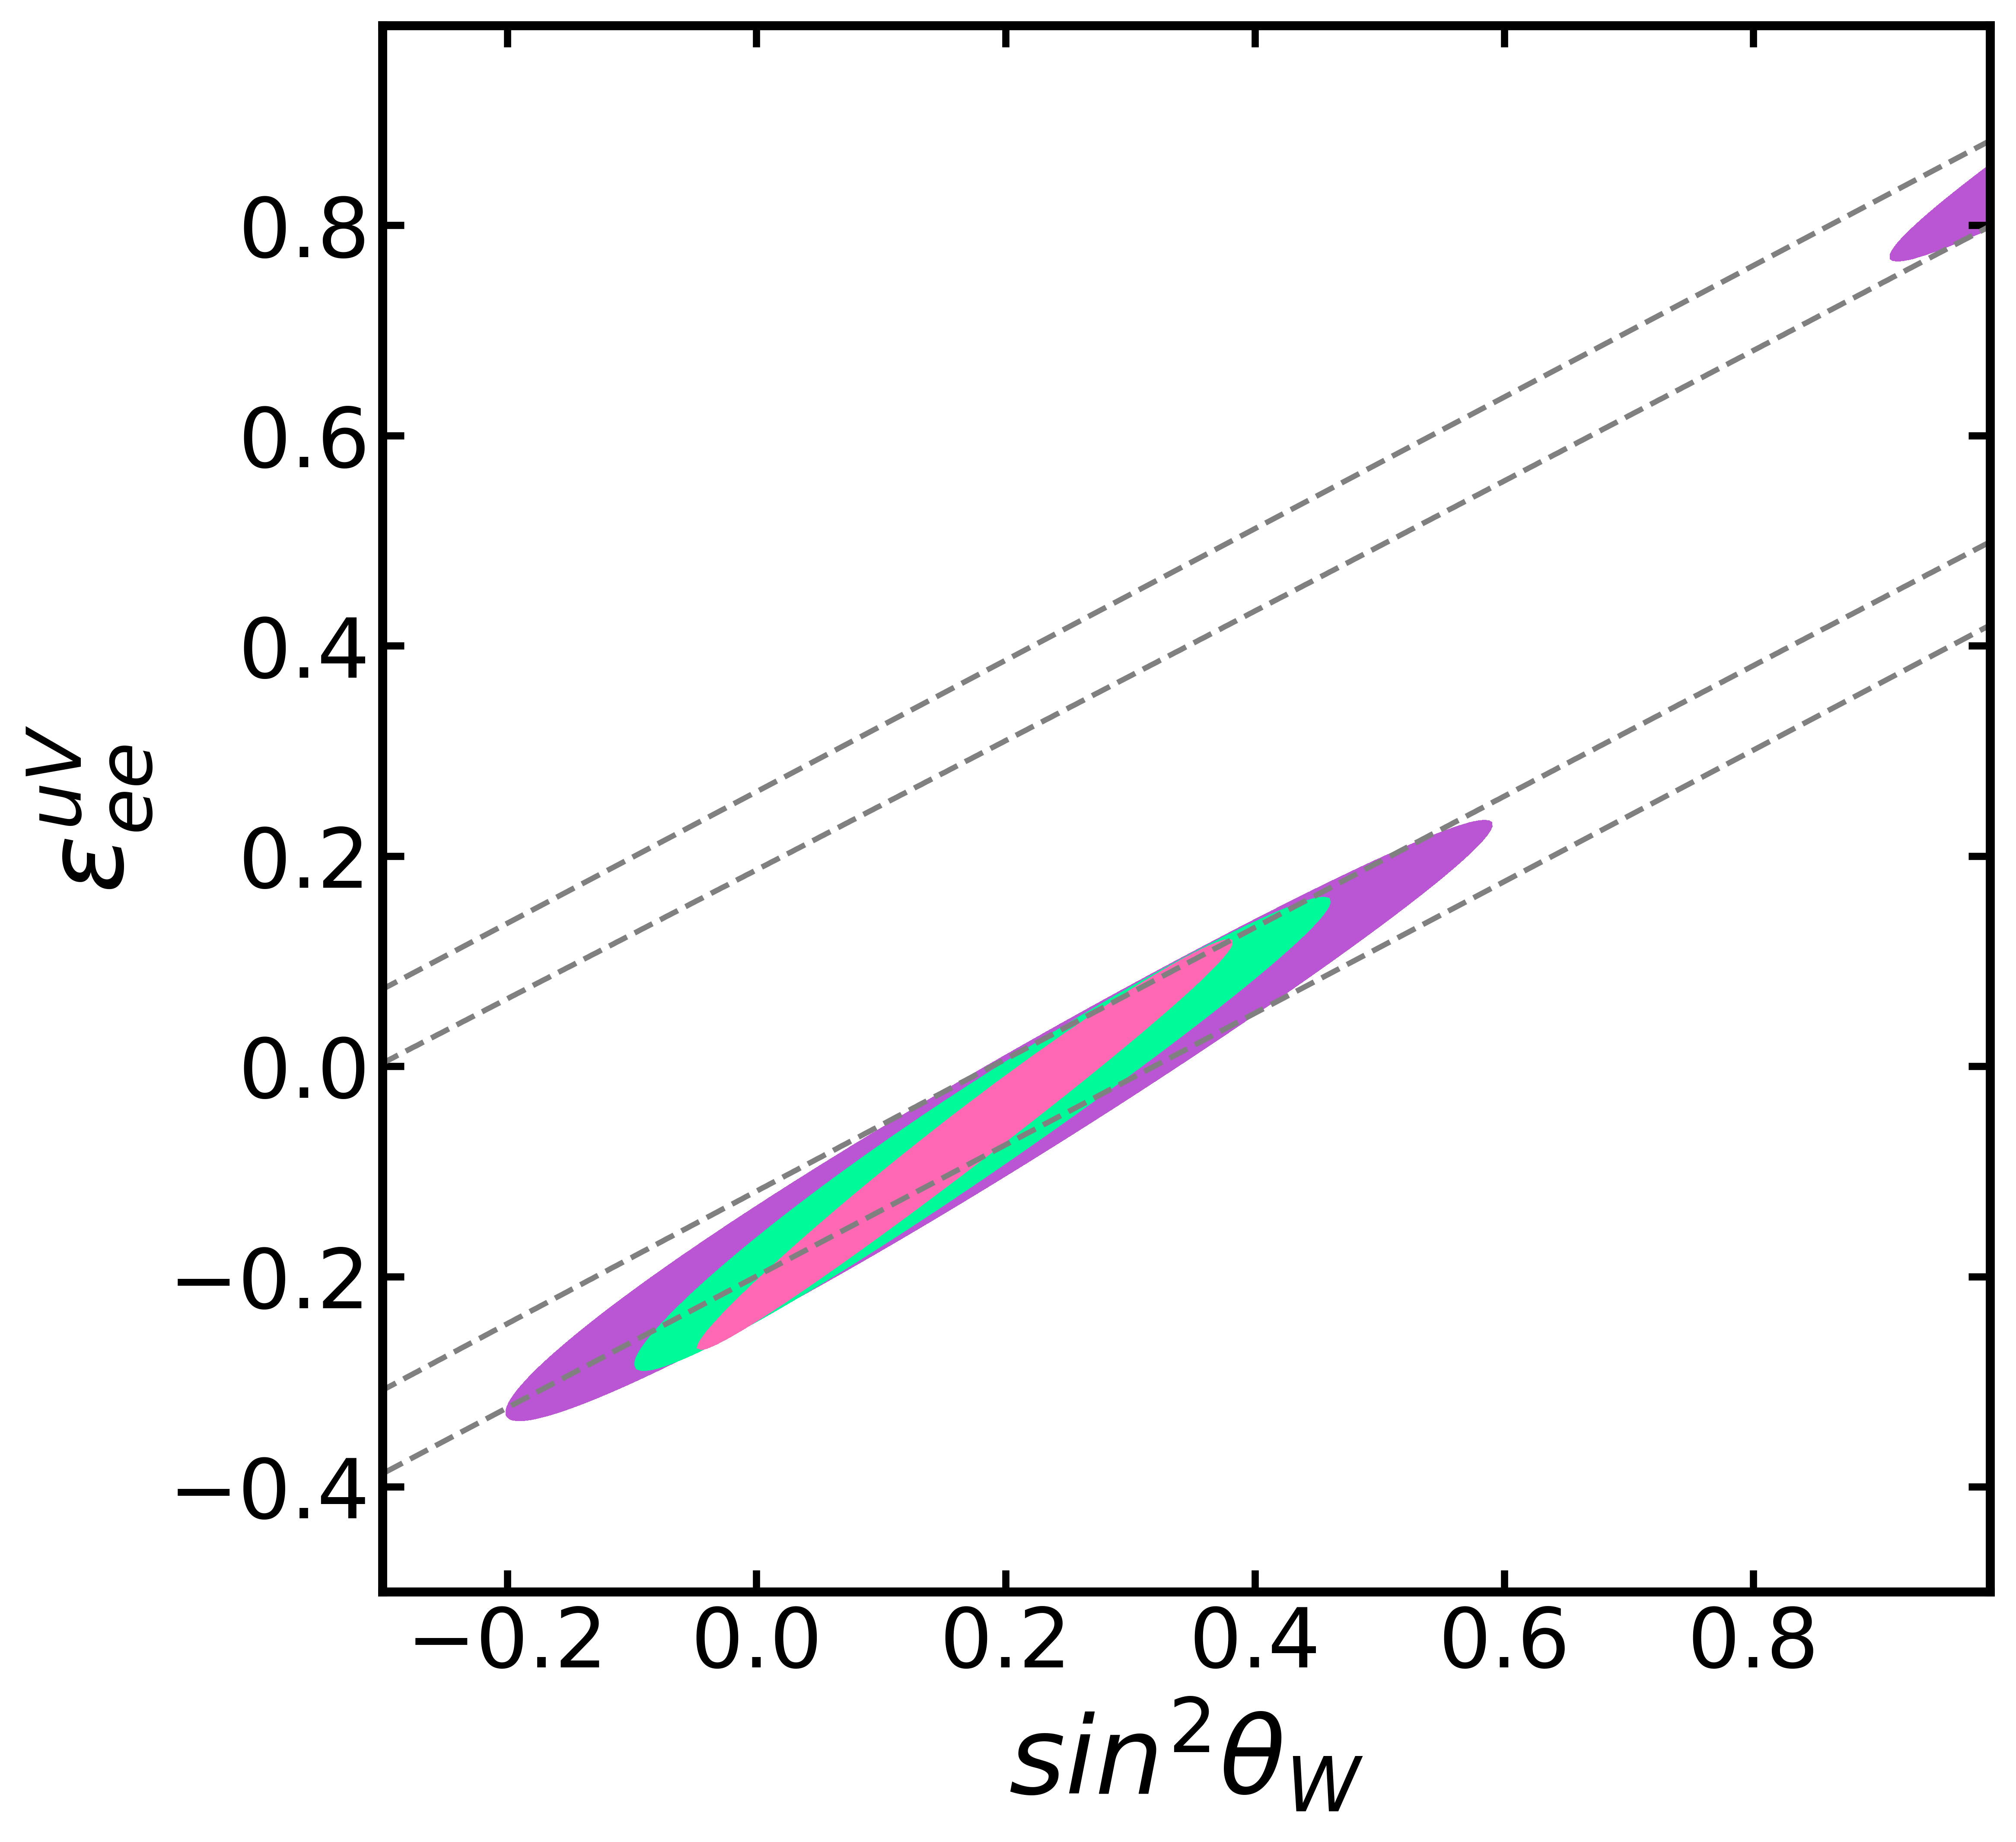
\includegraphics[scale=0.283]{figures/NSIZnU.png}}\hspace{0em}%
\subfigure{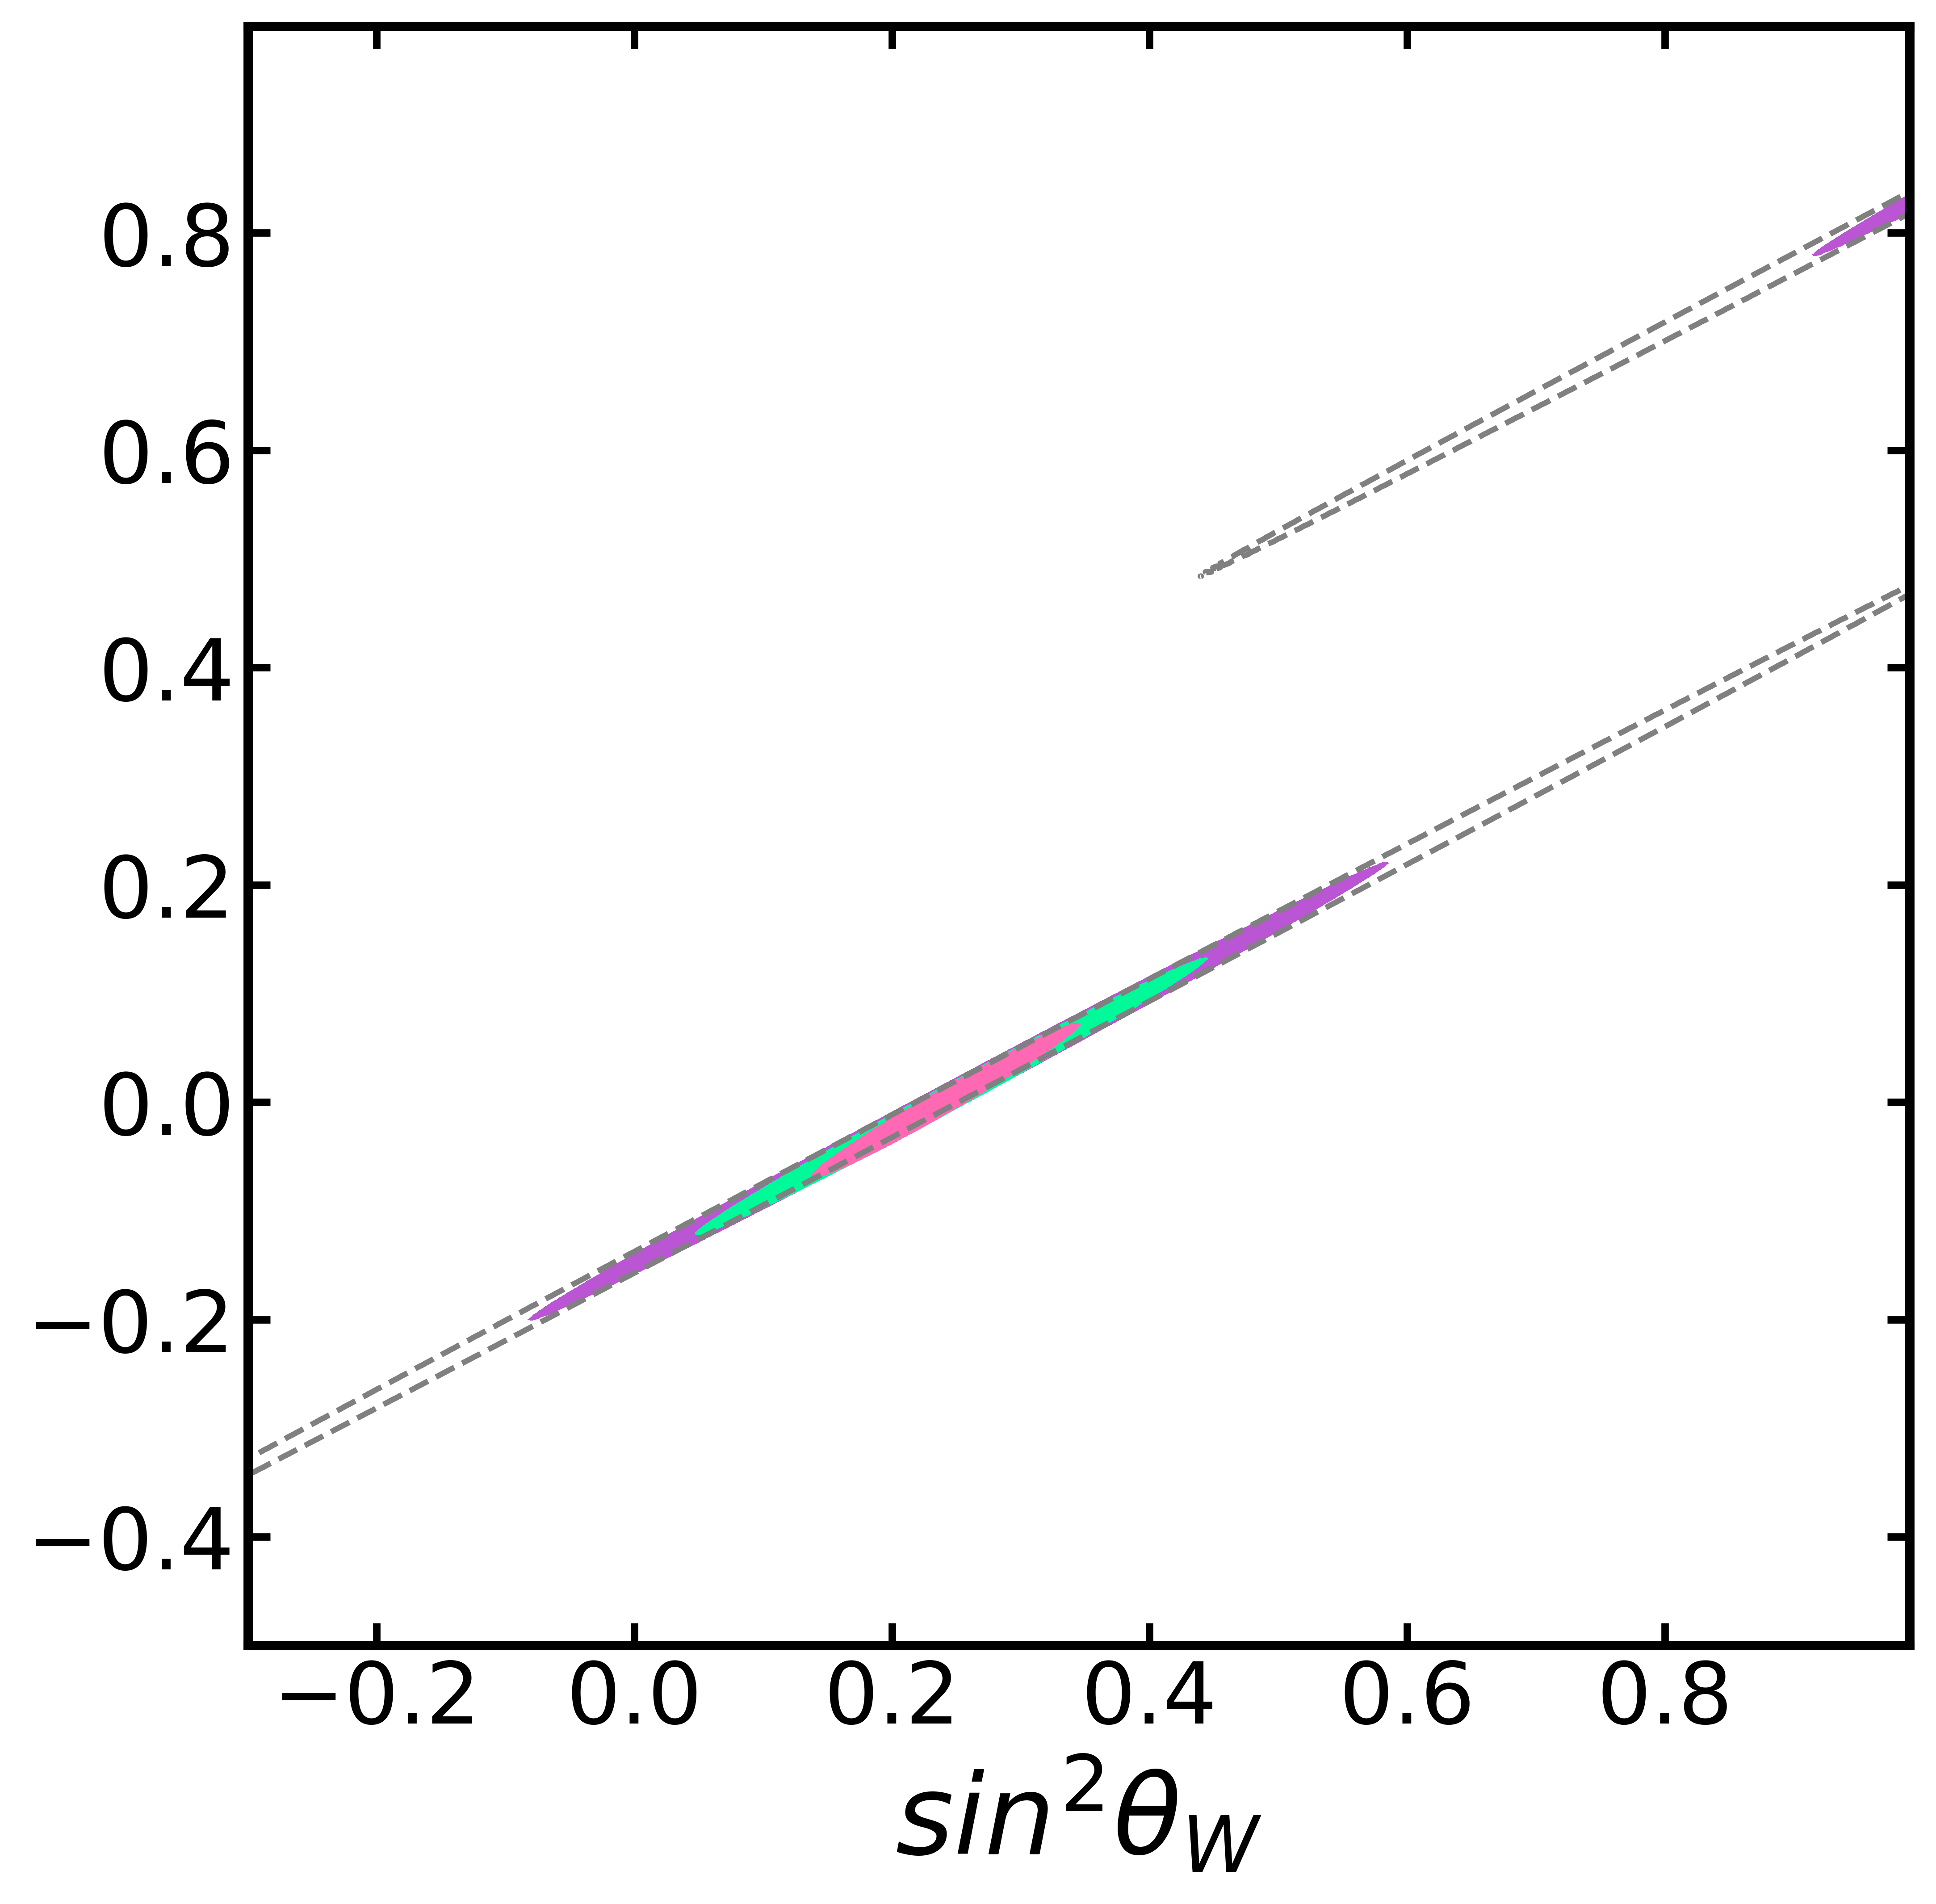
\includegraphics[scale=0.283]{figures/NSIZnU5.png}}\hspace{0em}%
\subfigure{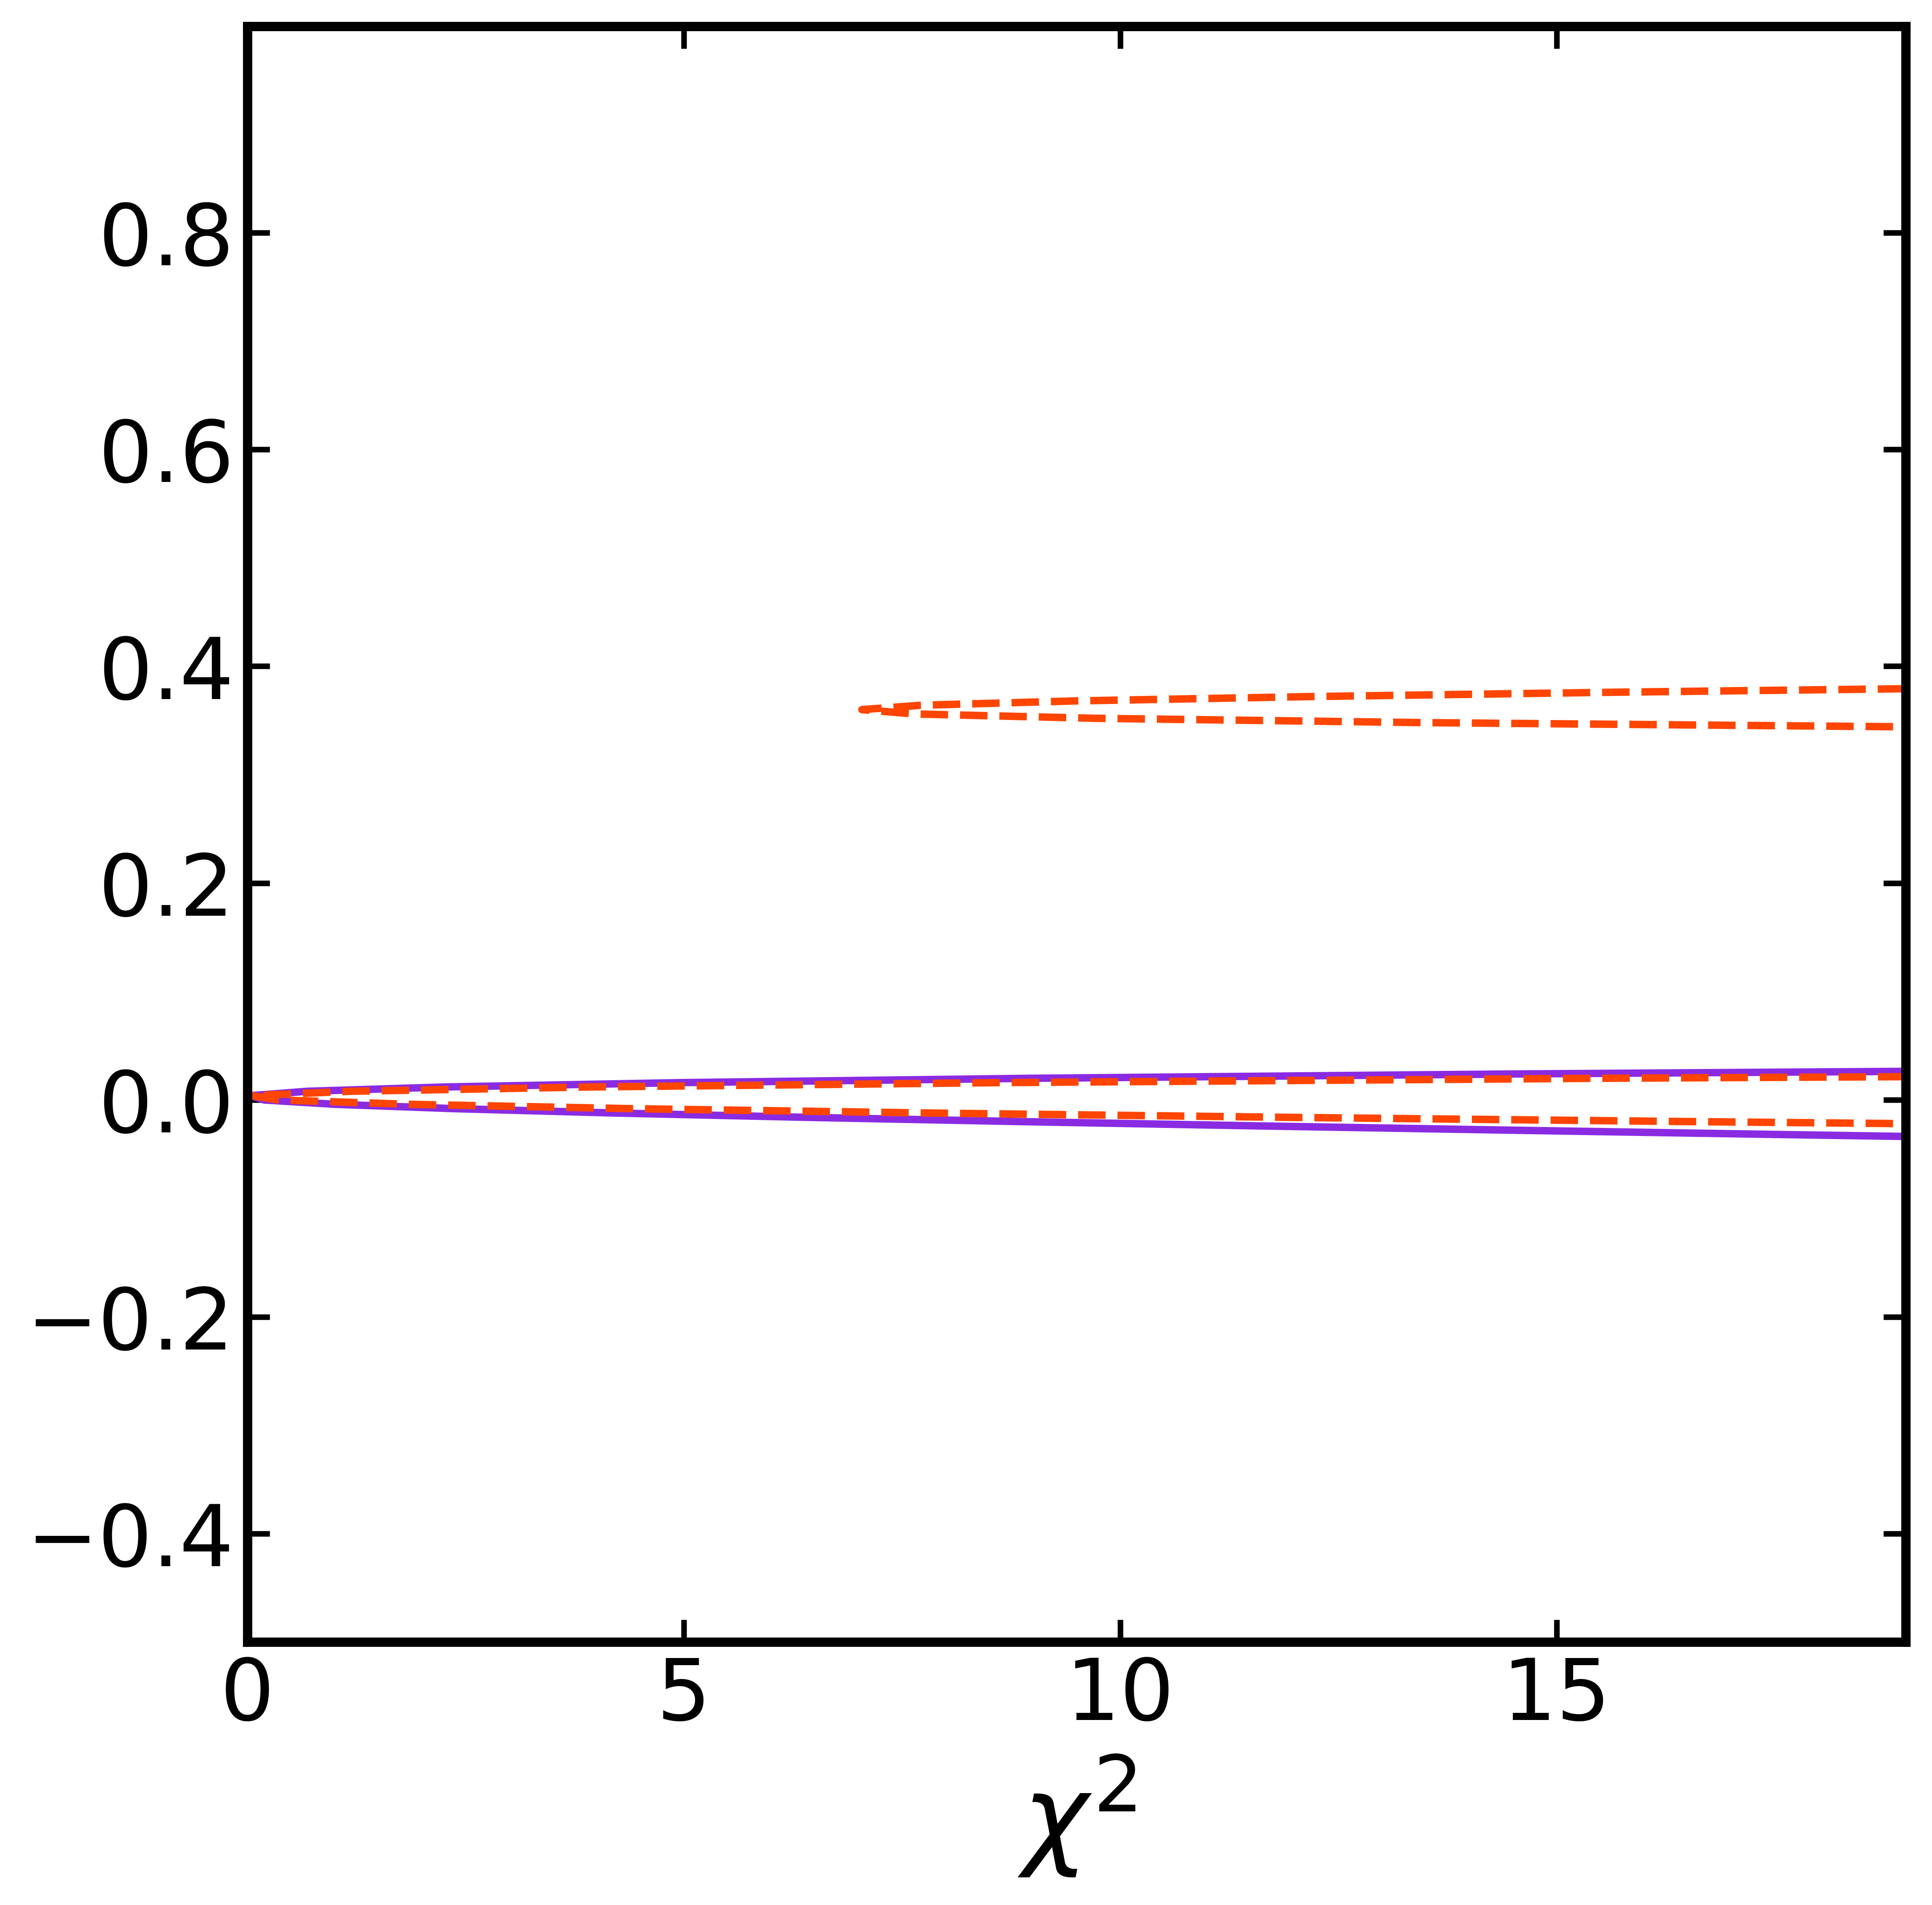
\includegraphics[scale=0.283]{figures/EeeuVZn.png}}
\caption{Expected allowed values for $sin^2\theta_W$ vs non-universal NSI parameters at a 90$\%$ confidence level for the Zn detectors exposed to a reactor antineutrino flux. The upper panel shows the space of $\varepsilon_{ee}^{dV}$ parameter, and the lower panel shows the space of $\varepsilon_{ee}^{uV}$ parameter.   The left side refers to the case of $\sigma_A=25\%$ and $\sigma_B=10\%$ , the central panels refer to the case of $\sigma_A=\sigma_B=5\%$, and the right side shows the analysis of the non-universal parameters for a fixed value of  $sin^2\theta_W$.  }
\label{WeakAngleZn}
\end{figure}

Finally, the case where both the weak mixing angle and non-universal NSI parameters vary was analyzed. Parameters related to interactions with the down and up quarks were considered. The results of this analysis are presented in Fig \ref{WeakAngleZn} for Zinc and Fig \ref{WeakAngleSi} for Silicon.  


Once again, the two cases of systematic errors considered in previous analyses were considered. It can be observed that the presence of these NSIs introduces a degeneracy in the values of the weak mixing angle. However, this degeneracy is broken when we consider our array of correlated detectors, and it even breaks within a small range for the uncorrelated case when the 5$\%$ systematic errors are considered.


Furthermore, the case where the value of the weak mixing angle is fixed, allowing only one NSI parameter to vary, is also presented. Here, degeneracies in this parameter can be observed, and the correlation between the proposed detectors can reduce them within specific ranges.






\begin{figure}[h!]
\centering
\subfigure{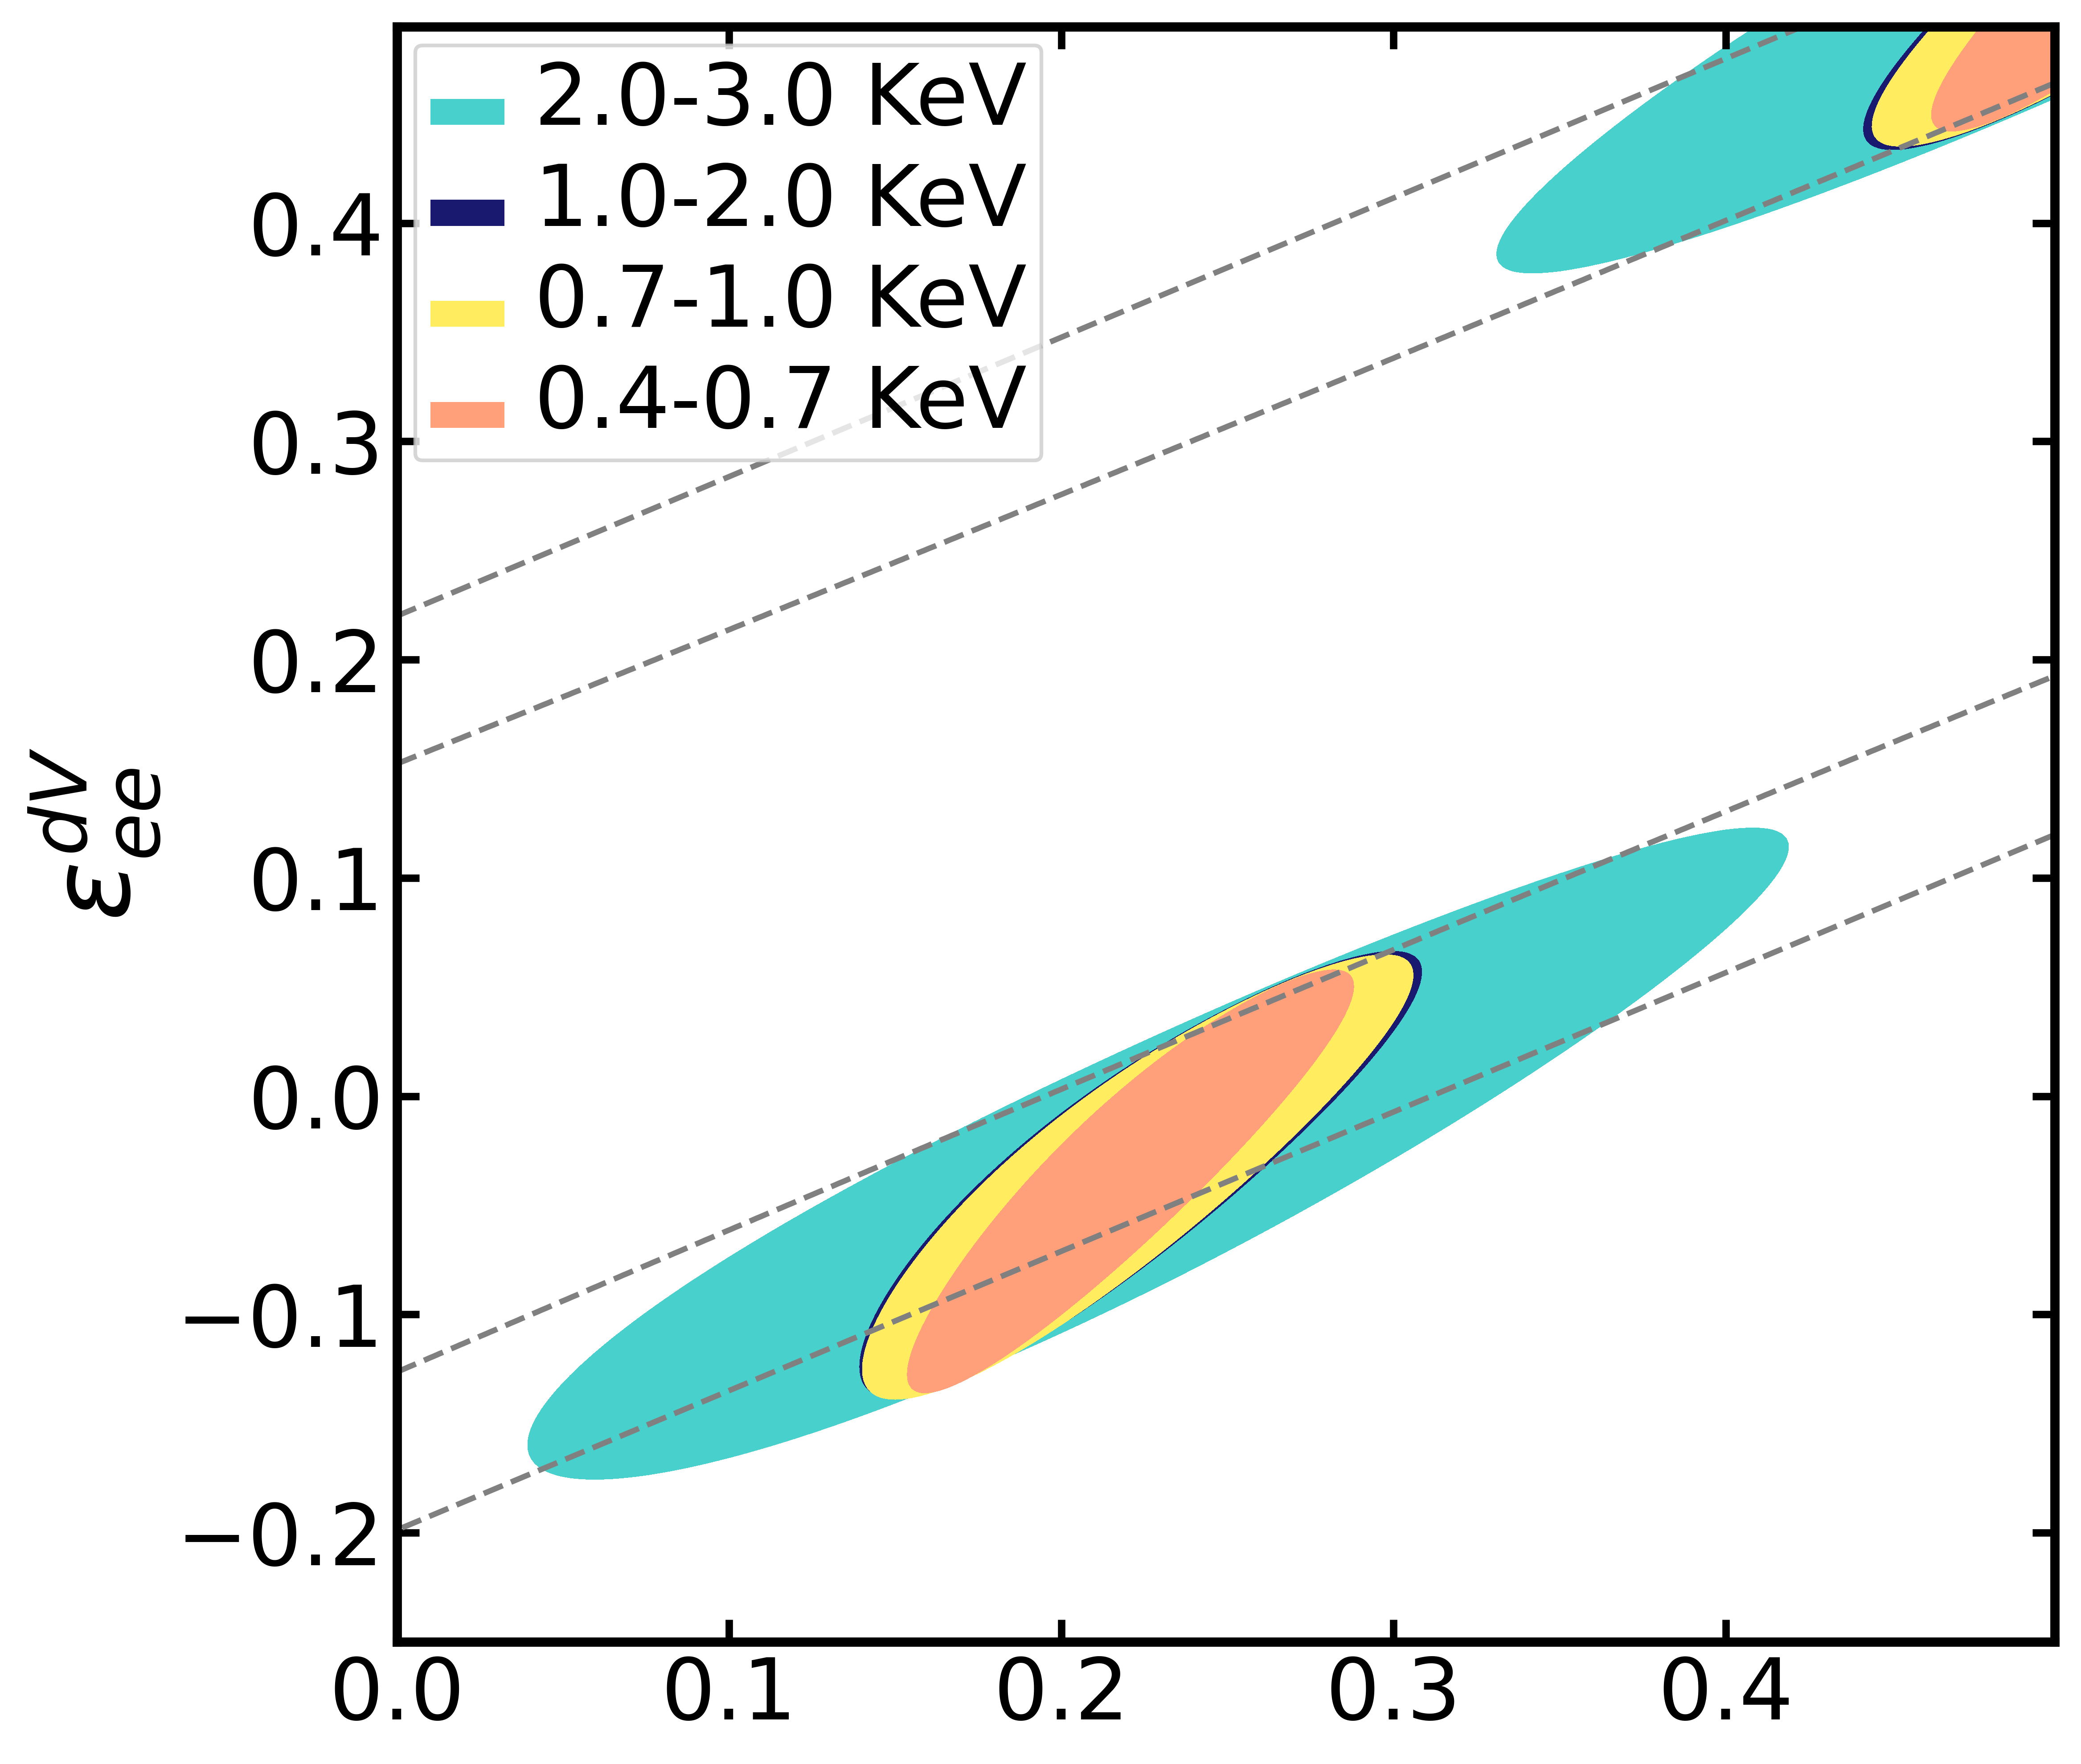
\includegraphics[scale=0.283]{figures/NSISi.png}}\hspace{0em}%
\subfigure{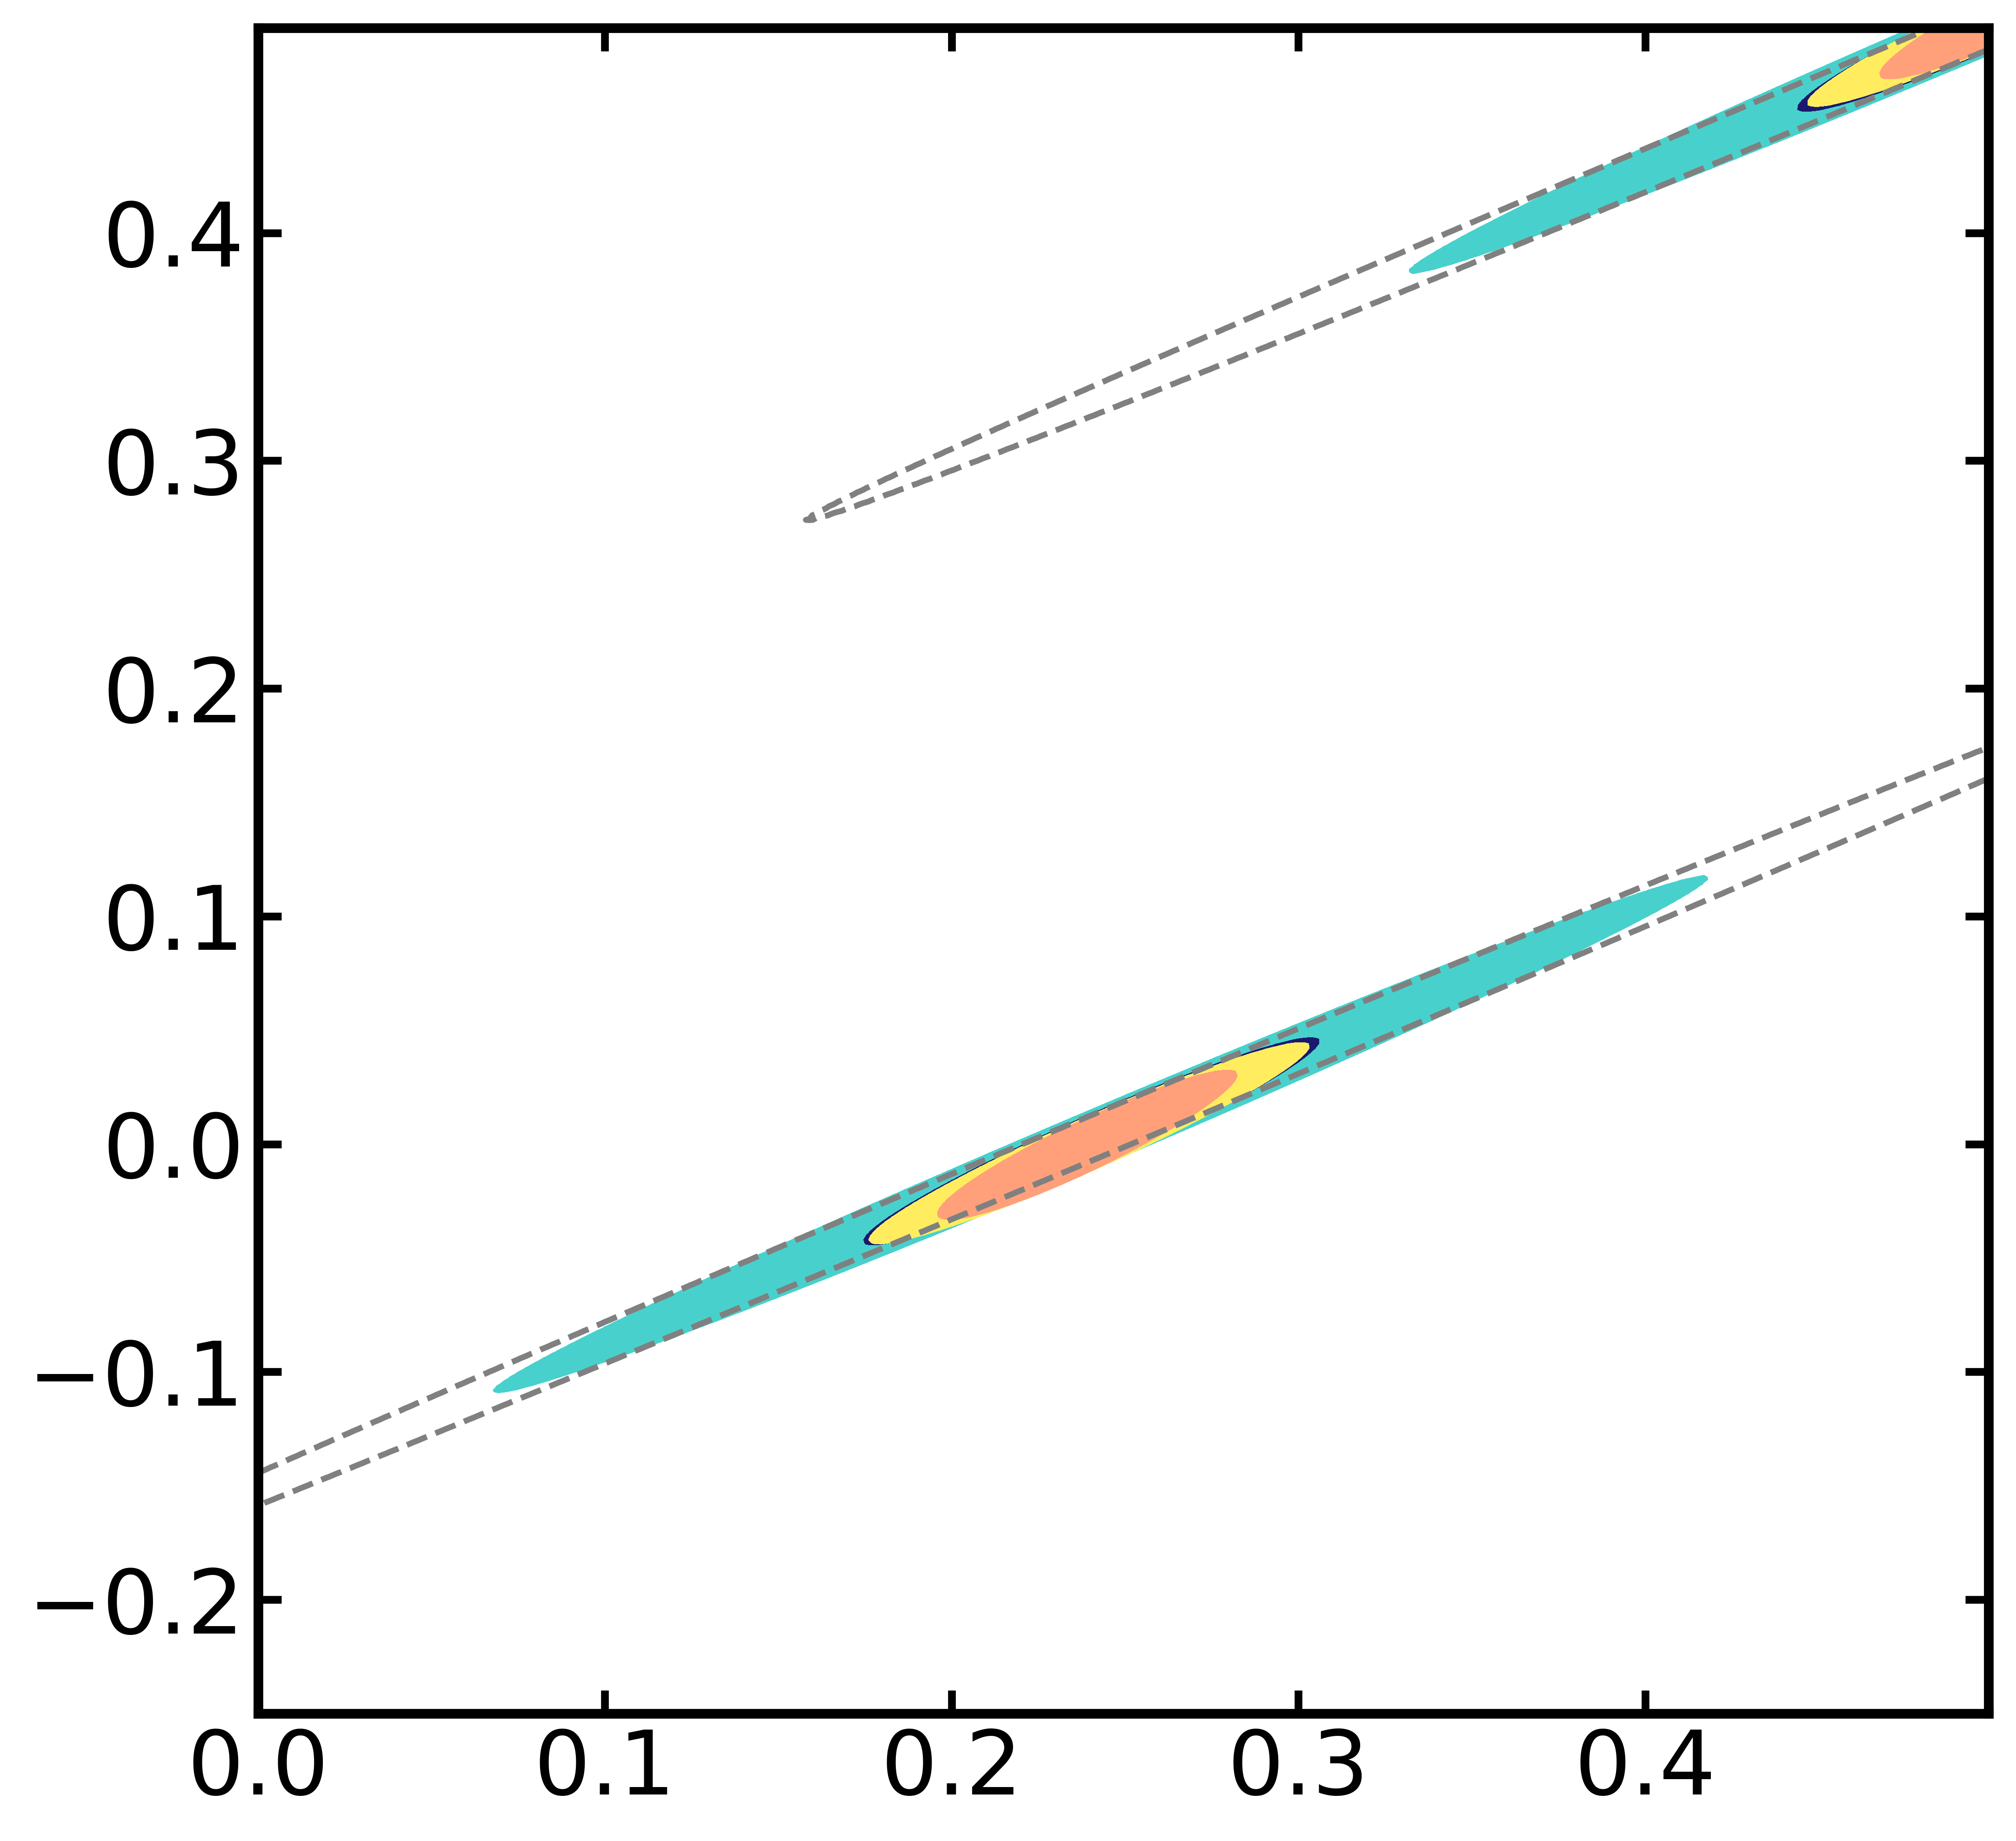
\includegraphics[scale=0.283]{figures/NSISi5.png}}\hspace{0em}%
\subfigure{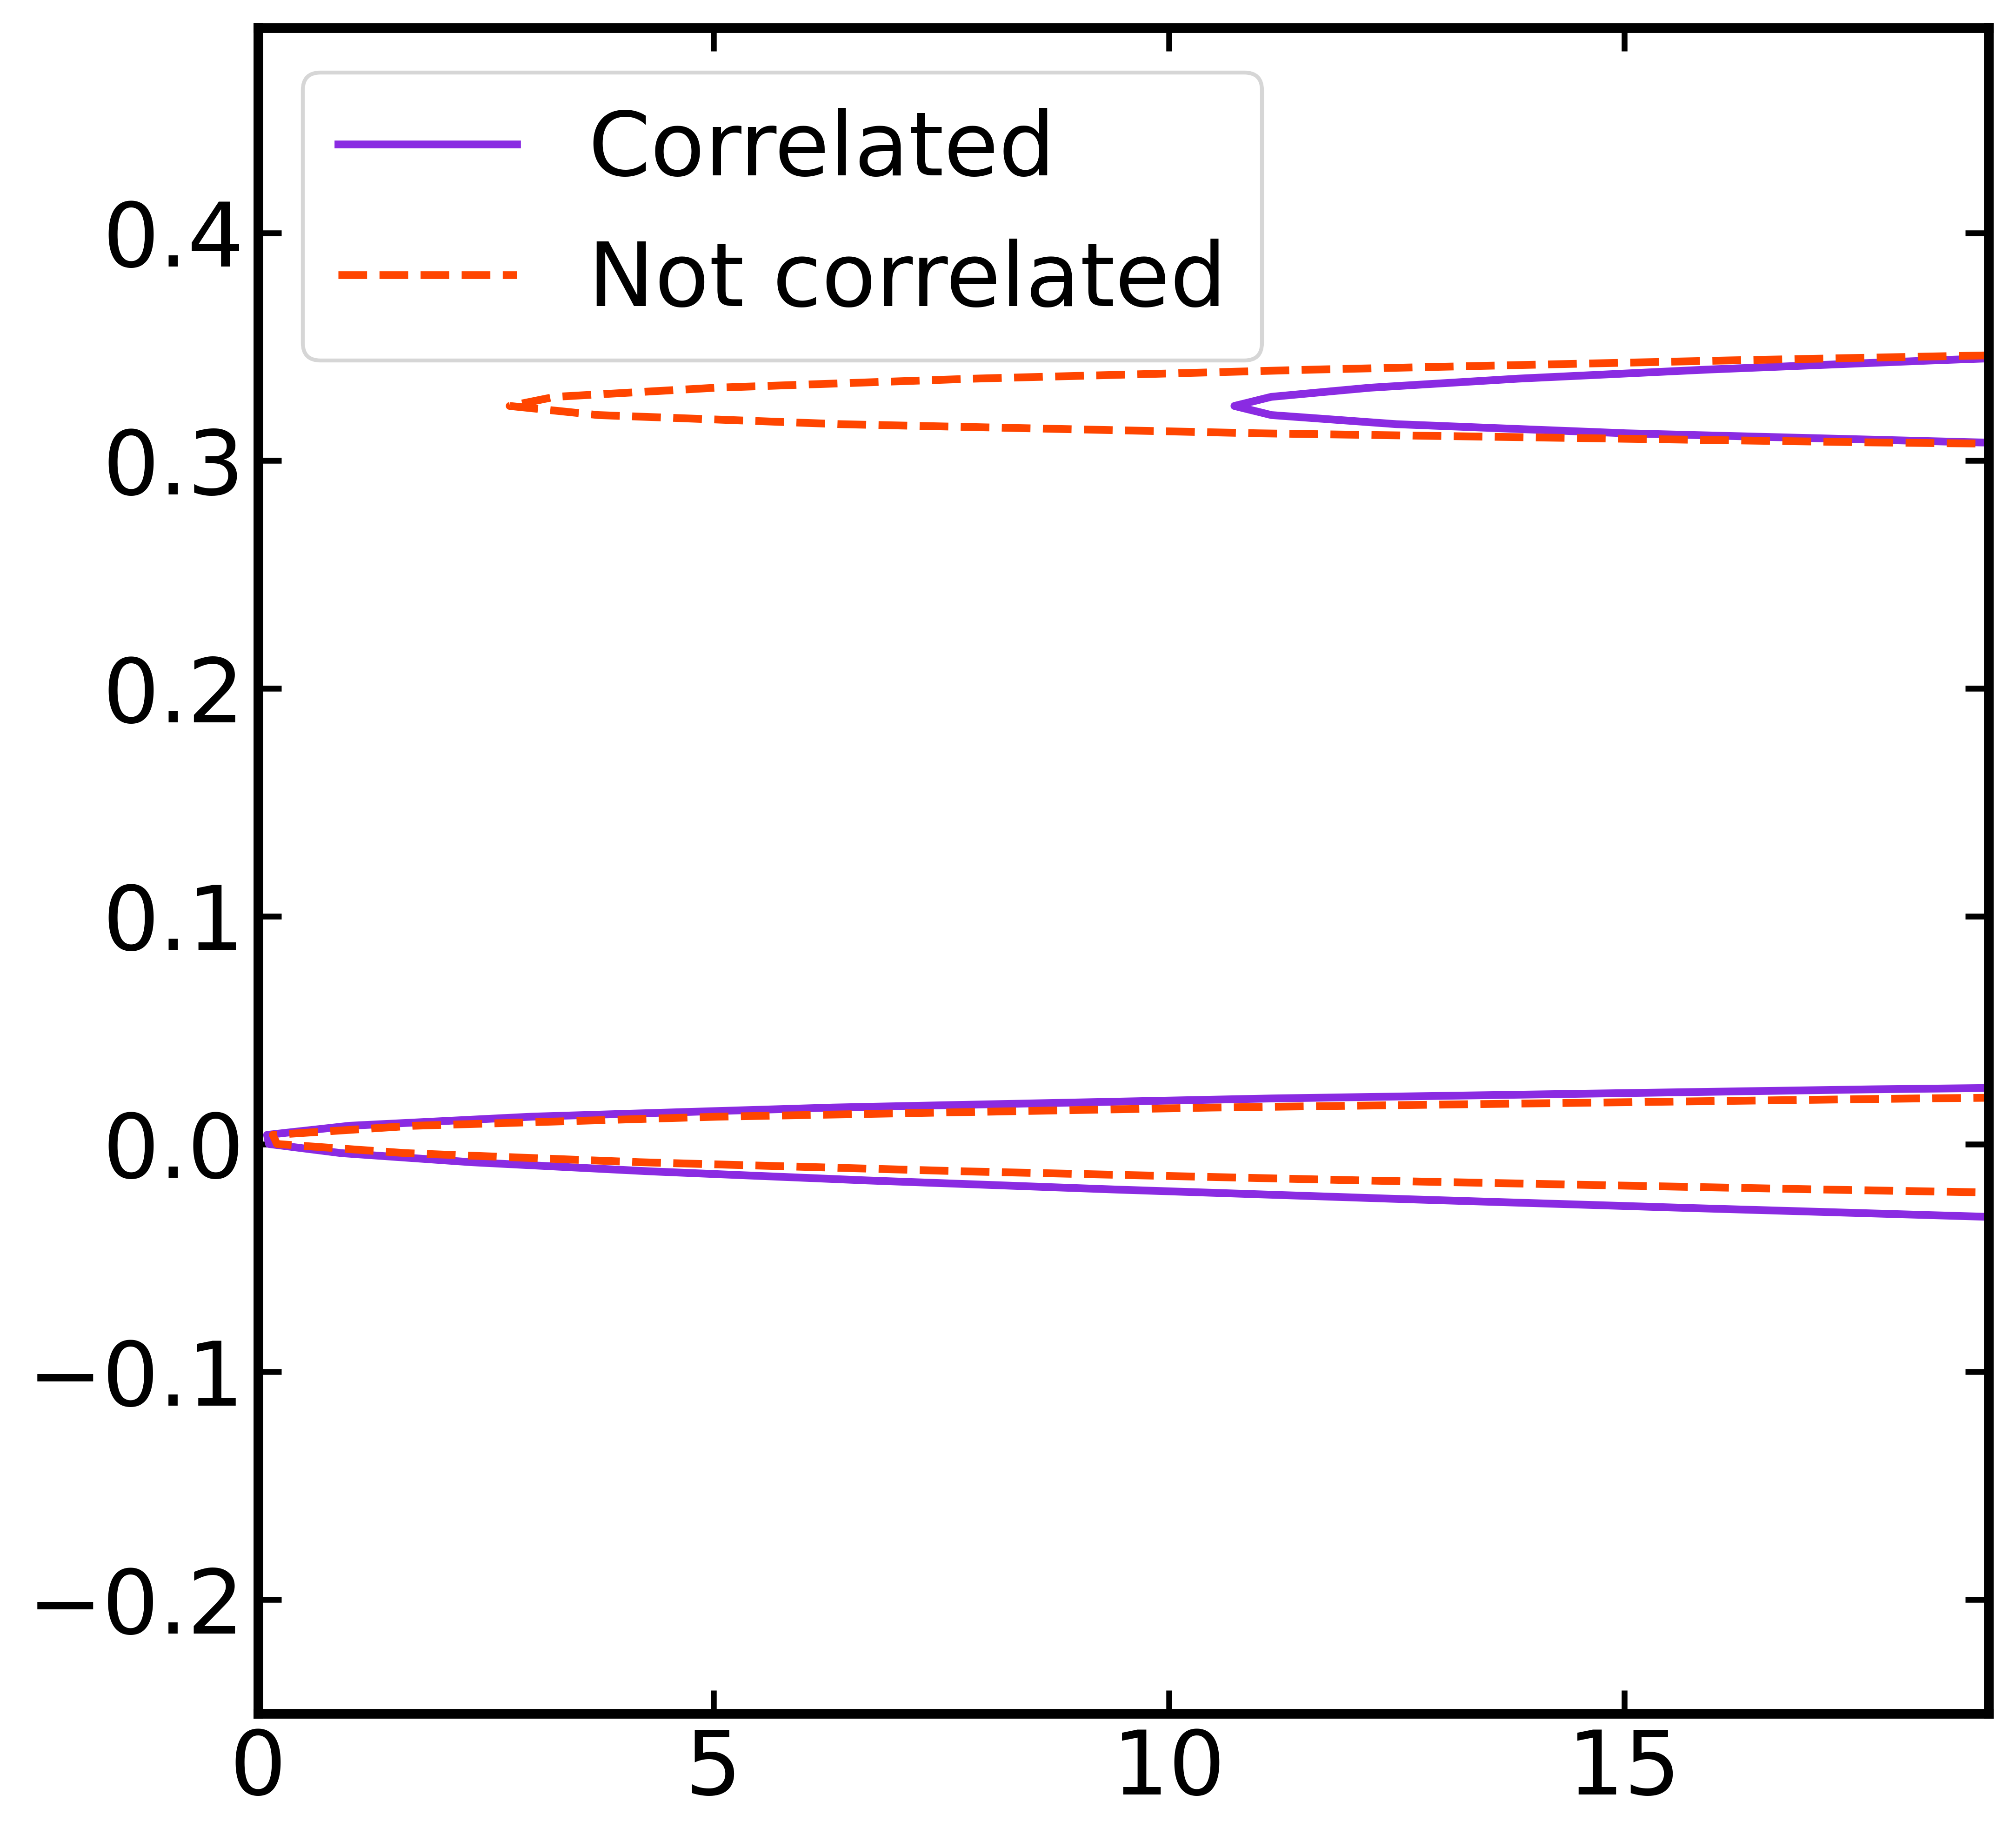
\includegraphics[scale=0.283]{figures/EeedVSi.png}}\par \vspace{-0.5em}
\subfigure{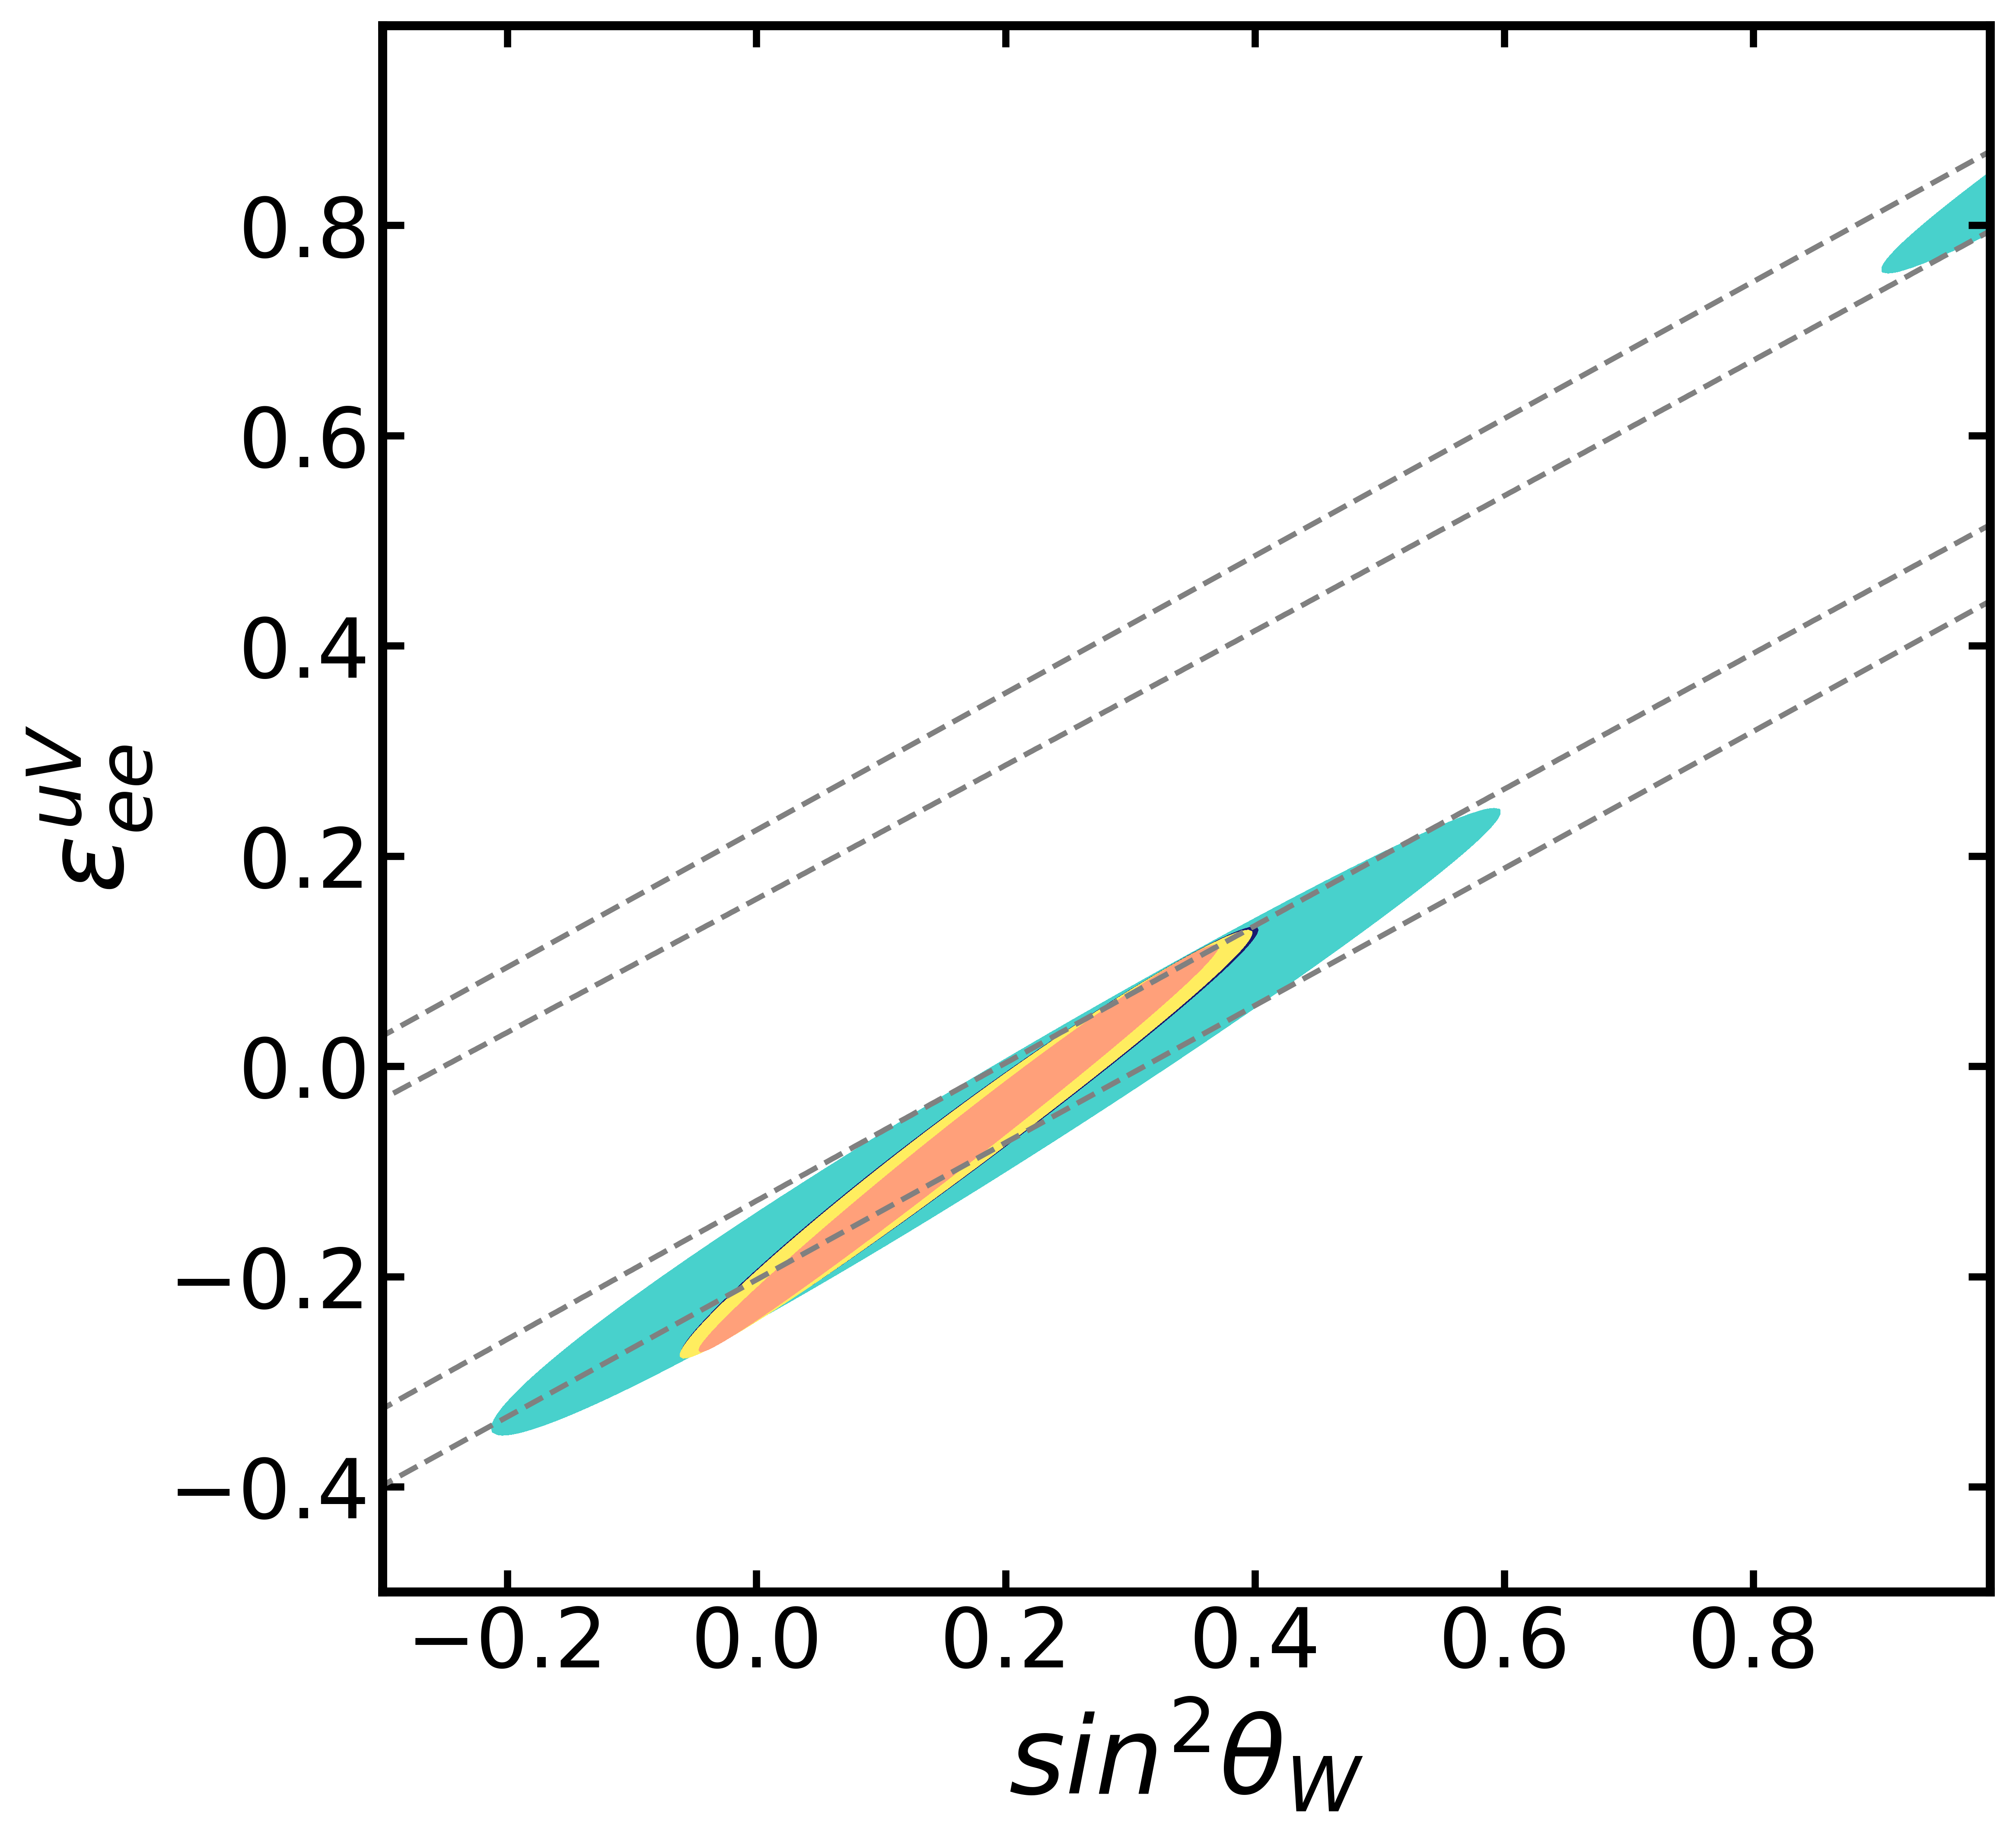
\includegraphics[scale=0.283]{figures/NSISiU.png}}\hspace{0em}%
\subfigure{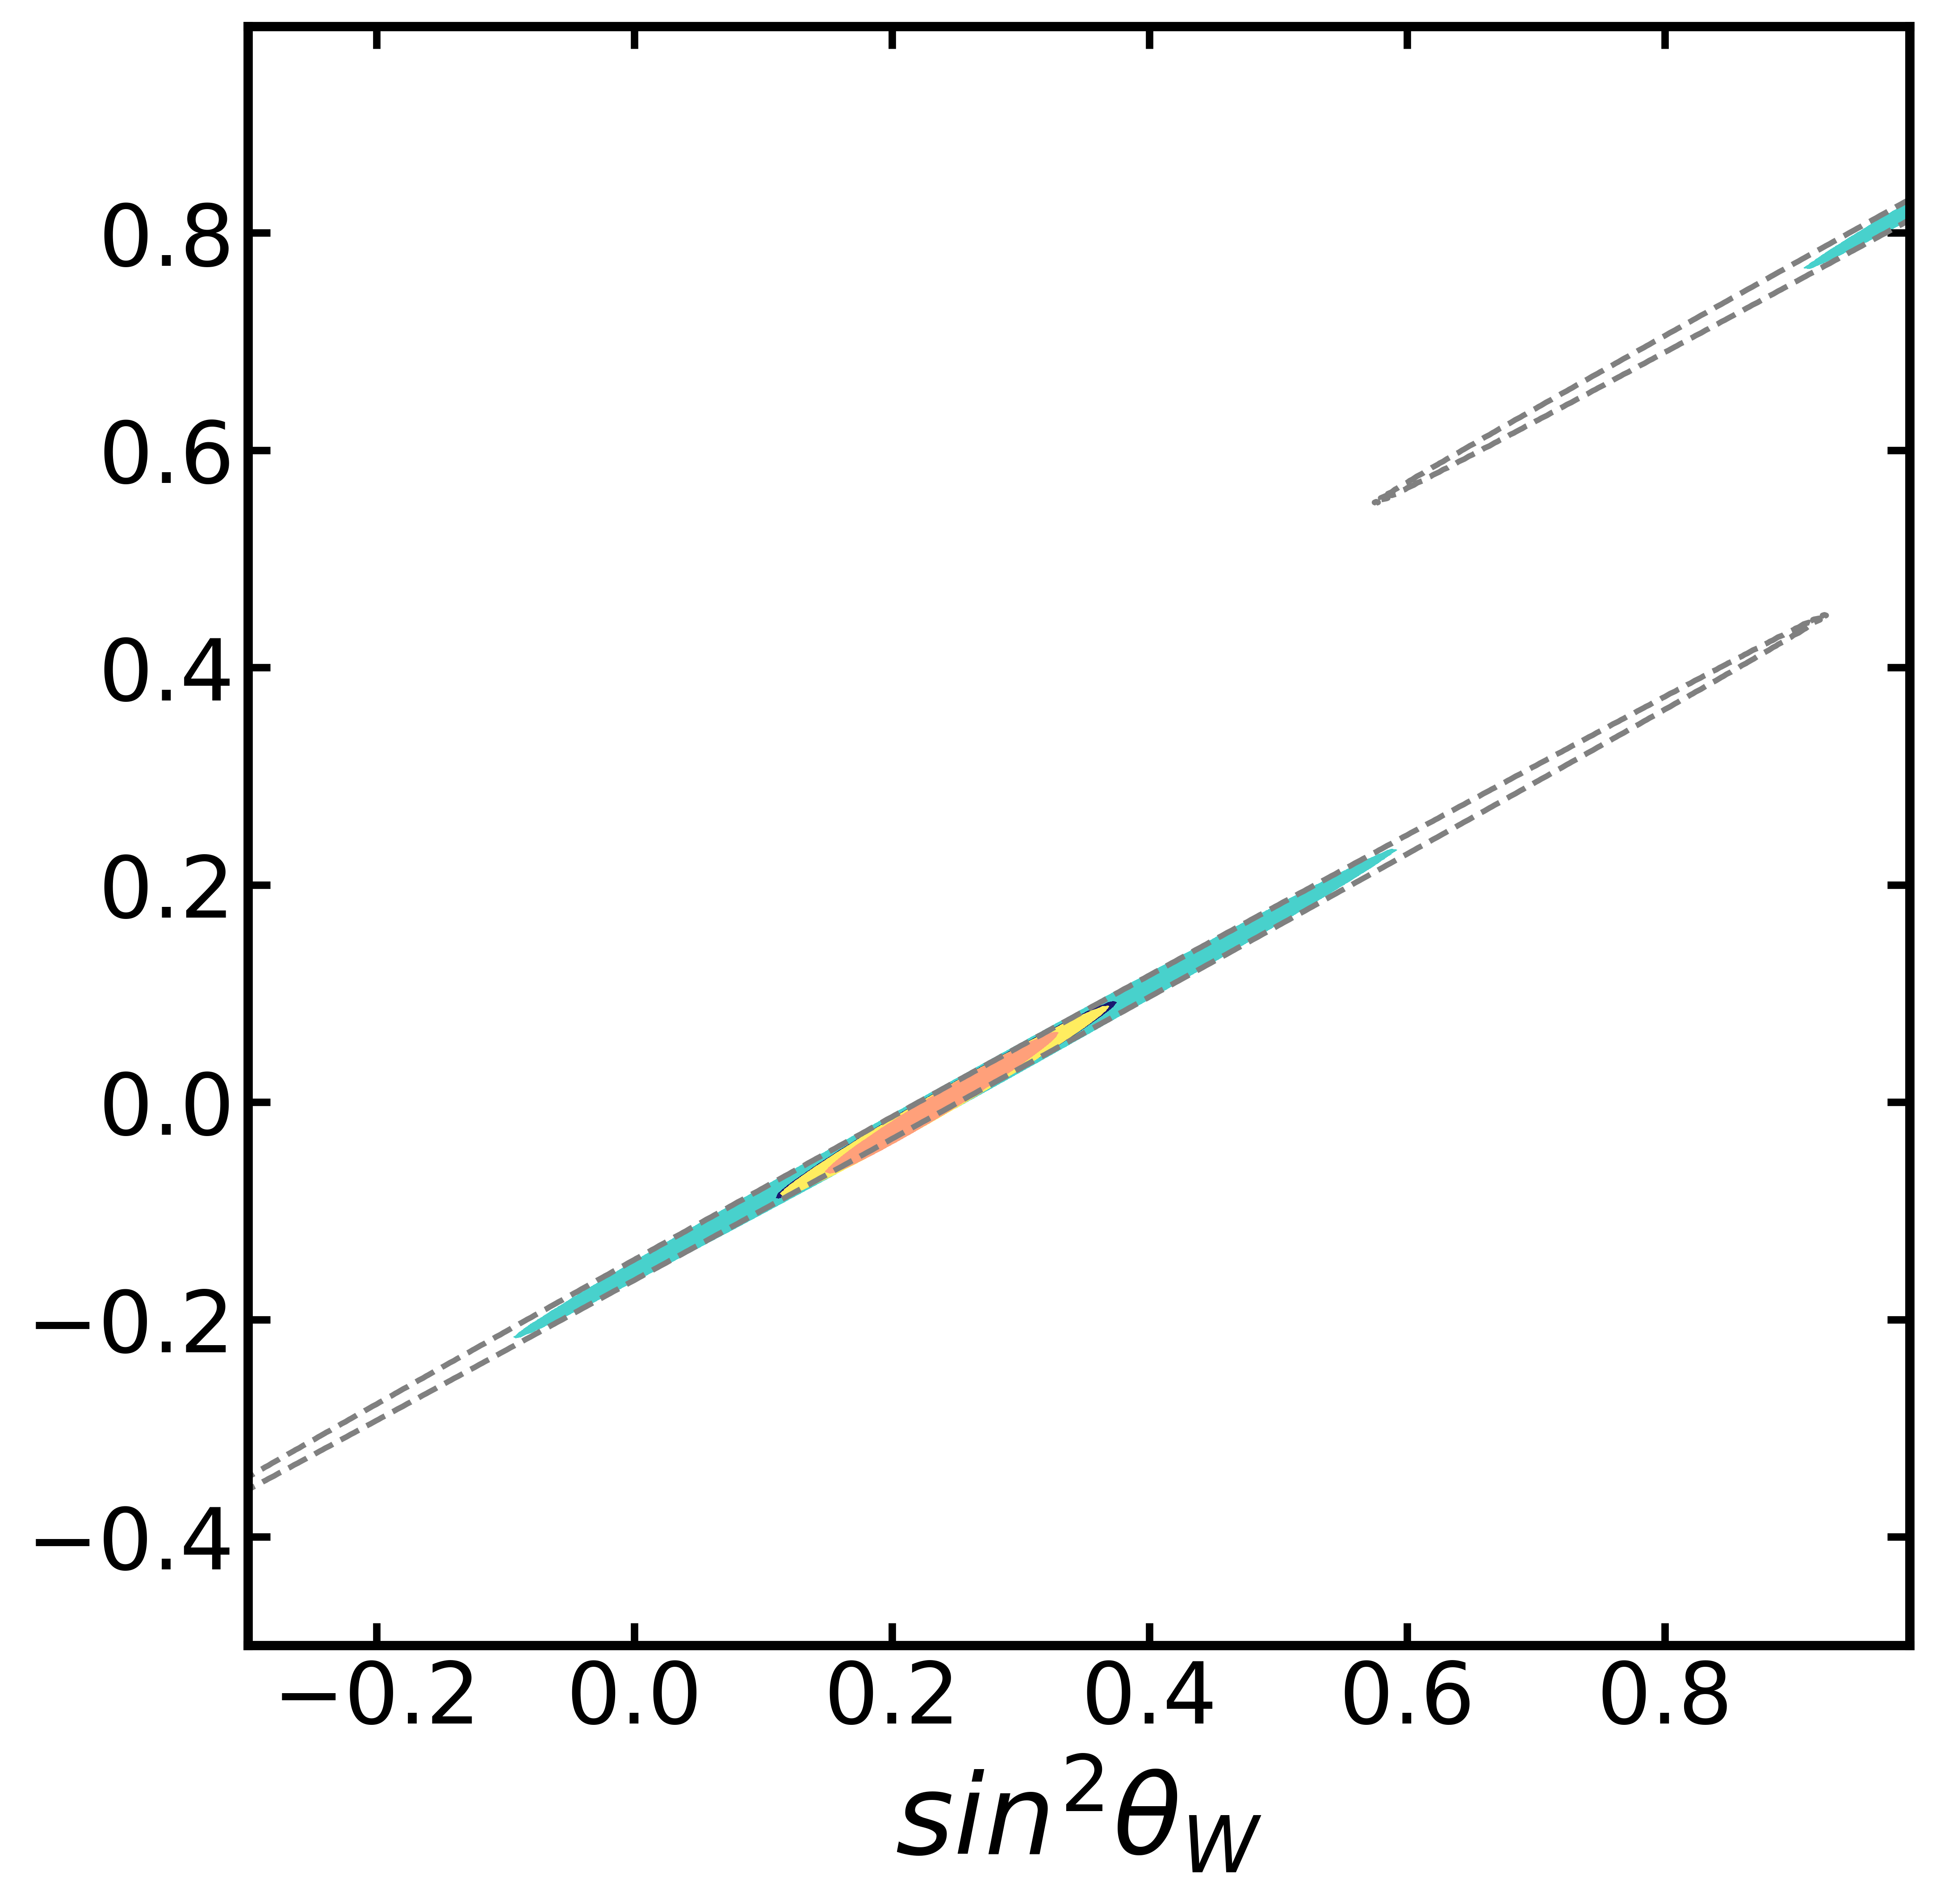
\includegraphics[scale=0.283]{figures/NSISiU5.png}}\hspace{0em}%
\subfigure{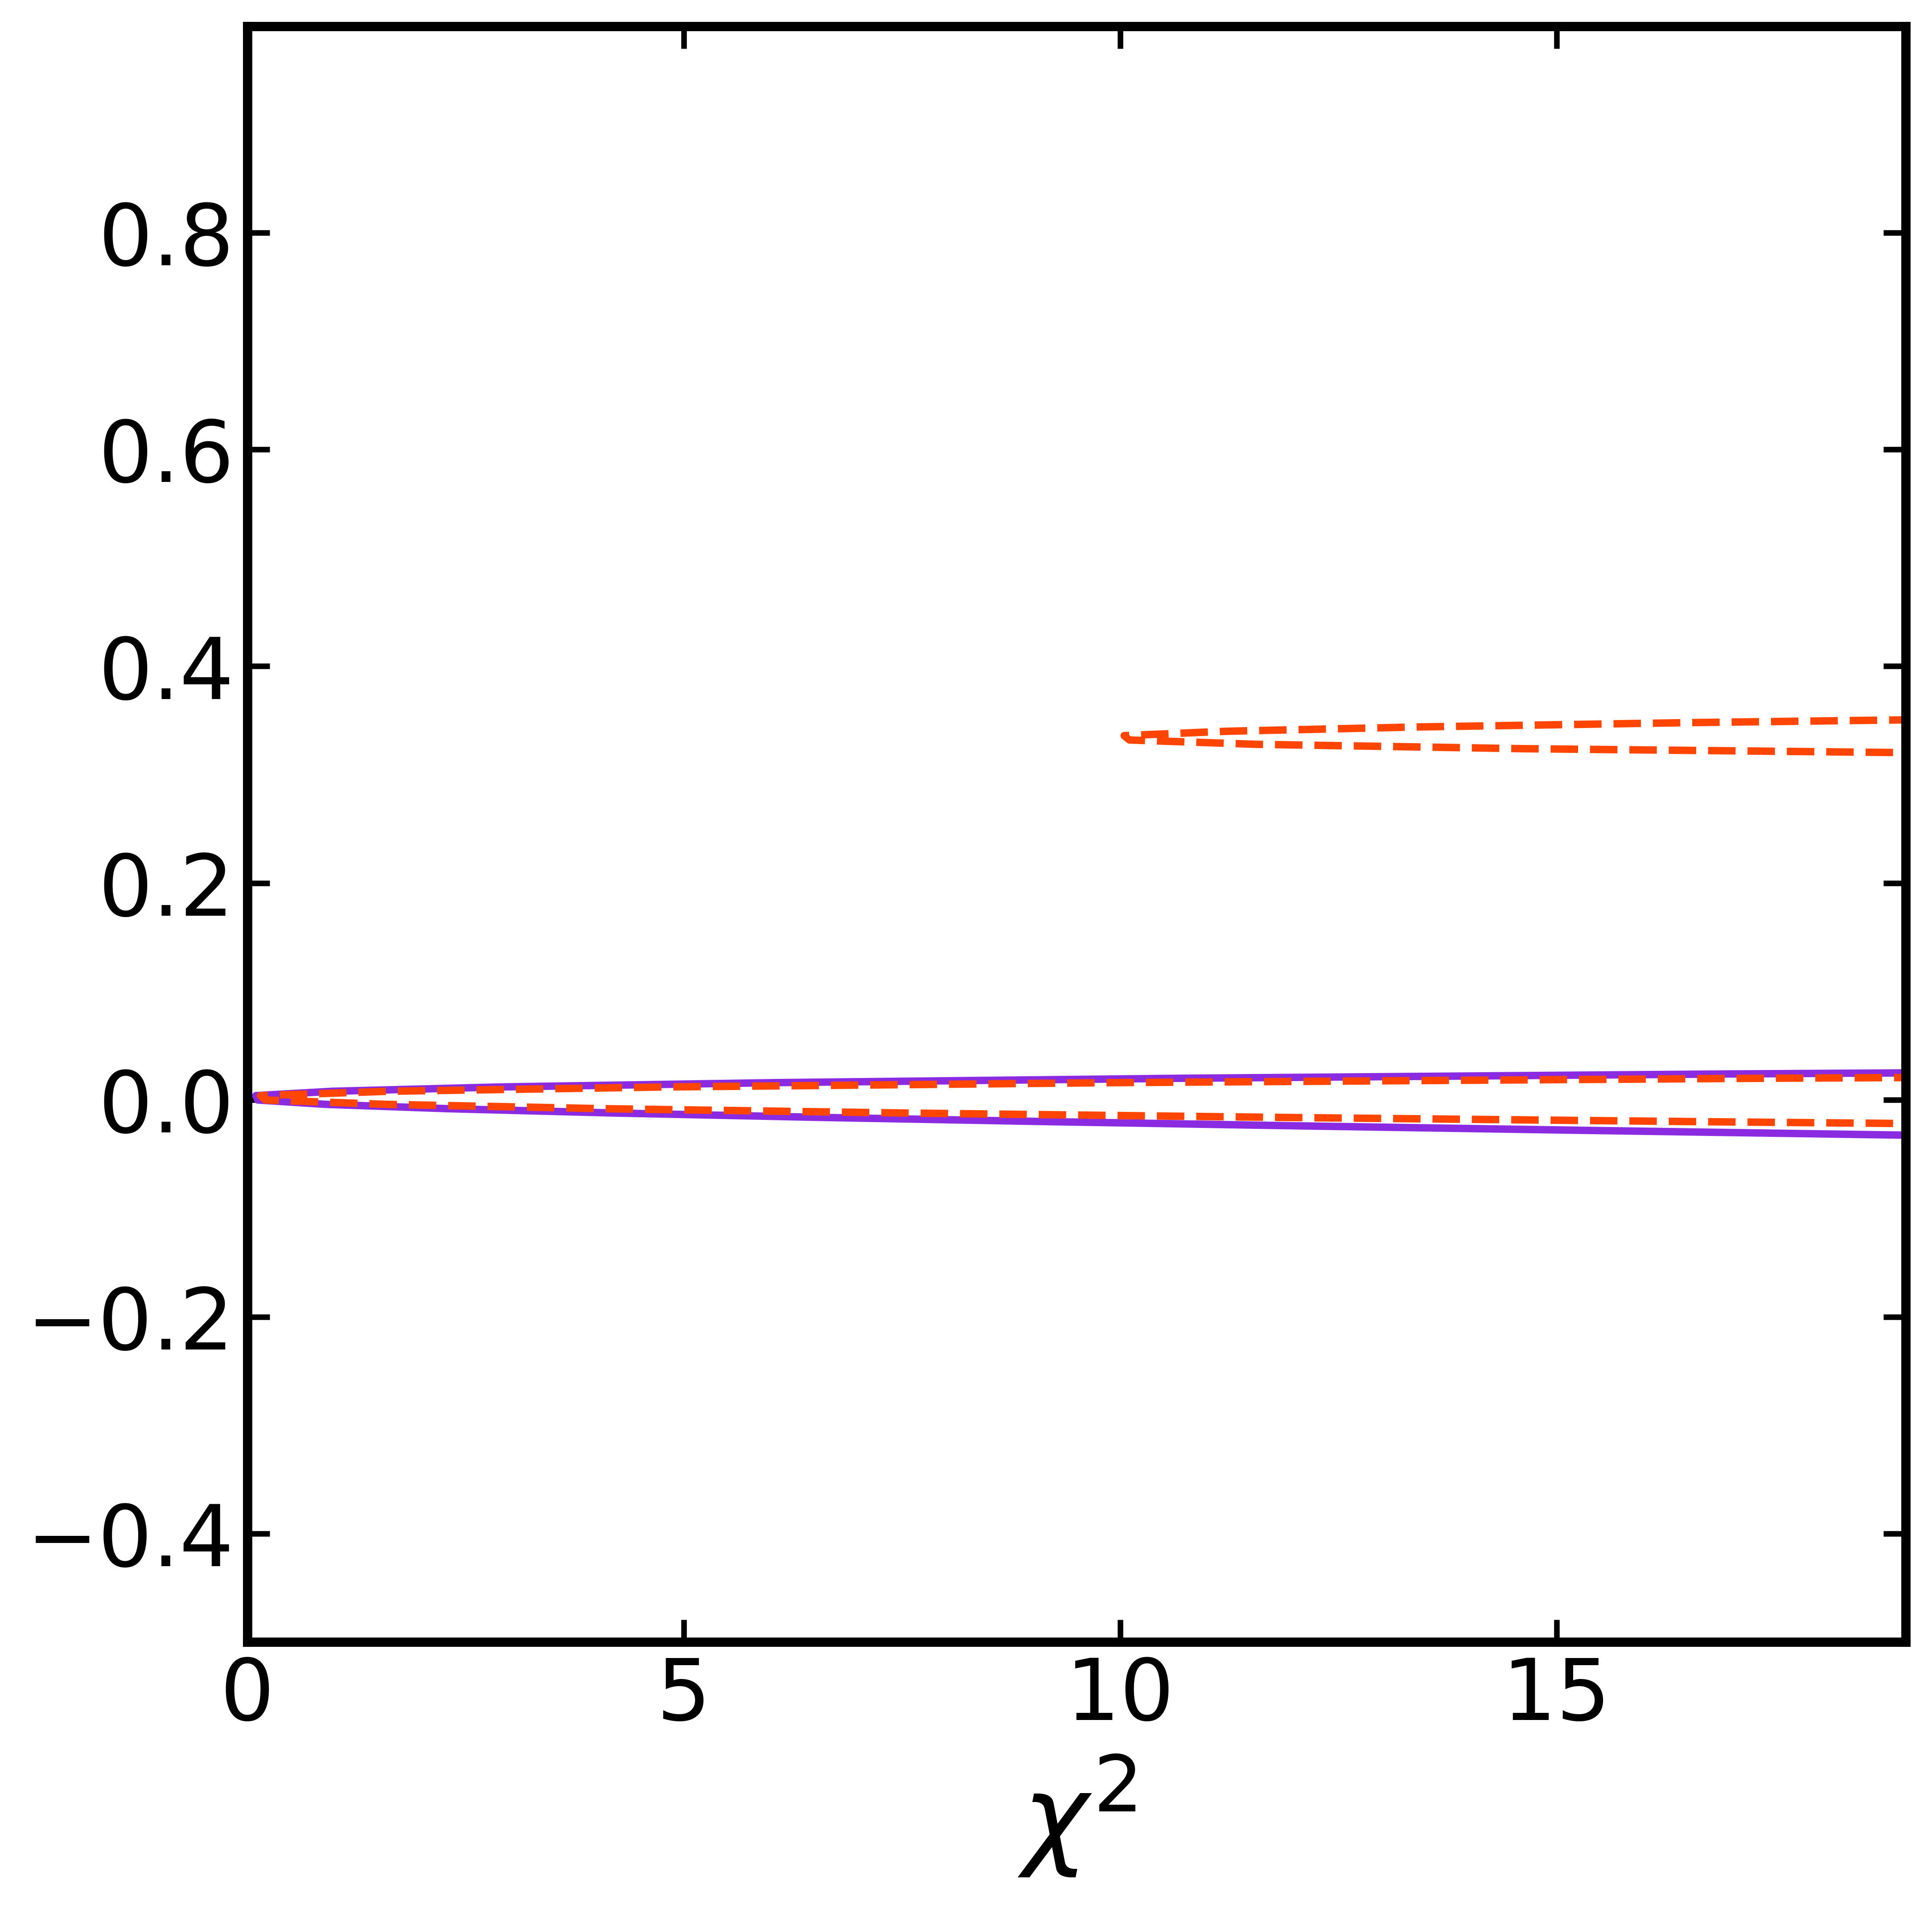
\includegraphics[scale=0.283]{figures/EeeuVSi.png}}
\caption{Expected allowed values for $sin^2\theta_W$ vs non-universal NSI parameters at a 90$\%$ confidence level for the Si detectors exposed to a reactor antineutrino flux. The upper panel shows the space of $\varepsilon_{ee}^{dV}$ parameter, and the lower panel shows the space of $\varepsilon_{ee}^{uV}$ parameter.   The left side refers to the case of $\sigma_A=25\%$ and $\sigma_B=10\%$ , the central panels refer to the case of $\sigma_A=\sigma_B=5\%$, and the right side shows the analysis of the non-universal parameters for a fixed value of  $sin^2\theta_W$.}
\label{WeakAngleSi}
\end{figure}







